% **************************************************************************************************************
% A Classic Thesis Style
% An Homage to The Elements of Typographic Style
%
% Copyright (C) 2010 Andr� Miede http://www.miede.de
%
% If you like the style then I would appreciate a postcard. My address 
% can be found in the file ClassicThesis.pdf. A collection of the 
% postcards I received so far is available online at 
% http://postcards.miede.de
%
% License:
% This program is free software; you can redistribute it and/or modify
% it under the terms of the GNU General Public License as published by
% the Free Software Foundation; either version 2 of the License, or
% (at your option) any later version.
%
% This program is distributed in the hope that it will be useful,
% but WITHOUT ANY WARRANTY; without even the implied warranty of
% MERCHANTABILITY or FITNESS FOR A PARTICULAR PURPOSE.  See the
% GNU General Public License for more details.
%
% You should have received a copy of the GNU General Public License
% along with this program; see the file COPYING.  If not, write to
% the Free Software Foundation, Inc., 59 Temple Place - Suite 330,
% Boston, MA 02111-1307, USA.
%
% **************************************************************************************************************
% Note:
%    * You must not use "u etc. in strings/commands that will be spaced out (use \"u or real umlauts instead)
%    * New enumeration (small caps): \begin{aenumerate} \end{aenumerate}
%    * For margin notes: \graffito{}
%    * Do not use bold fonts in this style, it is designed around them
%    * Use tables as in the examples
%    * See classicthesis-ldpkg.sty for useful commands
% **************************************************************************************************************
% To Do:
%    * [high] Check this out: http://www.golatex.de/koma-script-warnung-in-verbindung-mit-listings-package-t2058.html
%    * [medium] mathbb in section-titles/chapter-titles => disappears somehow in headlines!!!
%    * [low] Calculate text block size for Libertine font
%    * [low] Think about processing a4paper, a5paper, 10pt, 11pt, 12pt etc. options for typearea layout
%            (store values in internal variables and handle by \AtEndOfPackage{\areaset...})
% **************************************************************************************************************
\documentclass[ twoside,openright,titlepage,fleqn,numbers=noenddot,headinclude,%1headlines,footinclude
                11pt,letterpaper,BCOR5mm,cleardoublepage=empty,abstractoff % <--- obsolete, remove (todo)
                ]{scrreprt}
% ********************************************************************
% Development Stuff
% ********************************************************************
\listfiles
%\usepackage[l2tabu, orthodox, abort]{nag}
%\usepackage[warning, all]{onlyamsmath}
% ********************************************************************
% Re-usable information
% ********************************************************************
\newcommand{\myTitle}{A Substrate for Accountable Layered Systems\xspace}
\newcommand{\myDegree}{PhD in the Media Arts and Sciences\xspace}
\newcommand{\myName}{Bo Morgan\xspace}
\newcommand{\myProf}{Marvin Minsky\xspace}
\newcommand{\myOtherProf}{Gerald Sussman\xspace}
\newcommand{\mySupervisor}{Joseph Paradiso\xspace}
\newcommand{\myFaculty}{Put data here\xspace}
\newcommand{\myDepartment}{Media Lab\xspace}
\newcommand{\myUni}{\protect{Massachusetts Institute of Technology}\xspace}
\newcommand{\myLocation}{Cambridge\xspace}
\newcommand{\myTime}{June 2013\xspace}
\newcommand{\myVersion}{Version 1.0\xspace}
%*******************************************************
% Packages with options that might require adjustments
%*******************************************************
\usepackage[latin1]{inputenc}
\usepackage[ngerman,american]{babel}
\usepackage{natbib}
%\usepackage[square,numbers]{natbib}
\usepackage[fleqn]{amsmath} % math environments and more by the AMS

%*******************************************************
\usepackage{classicthesis-ldpkg} % [backref]
%*******************************************************
% Options for classicthesis.sty:
% tocaligned eulerchapternumbers drafting linedheaders listsseparated 
% subfig nochapters beramono eulermath parts minionpro pdfspacing 
% listings dottedtoc minionprospacing manychapters
\usepackage[eulerchapternumbers,listings,listsseparated,%pdfspacing,%listings,
            subfig,beramono,eulermath,parts,manychapters,dottedtoc]{classicthesis}

\usepackage{enumerate}

%*******************************************************
% Some font experiments
%*******************************************************
%\usepackage[osf]{libertine}
%\usepackage{hfoldsty}
%\usepackage[light,condensed,math]{iwona}
%\renewcommand{\sfdefault}{iwona}
%\usepackage{lmodern} % <-- no osf support :-(
%\usepackage[urw-garamond]{mathdesign} <-- no osf support :-(

%*******************************************************
% Fine-tuning for the text area
%*******************************************************
%\linespread{1.05} % a bit more for Palatino
%\areaset[5mm]{312pt}{761pt} % 686 (factor 2.2) + 33 head + 42 head \the\footskip
%\setlength{\marginparwidth}{7em}%
%\setlength{\marginparsep}{2em}%

% This is a drop-in replacement for \begin{enumerate}...\end{enumerate} in LaTeX. Just include it in
% your preamble and use \begin{packed_enum} instead.
\newenvironment{packed_enumerate}{
\begin{enumerate}
\setlength{\itemsep}{2.5pt}
\setlength{\parskip}{0pt}
\setlength{\parsep}{0pt}
}{\end{enumerate}}
\newenvironment{packed_itemize}{
\begin{itemize}
\setlength{\itemsep}{2.5pt}
\setlength{\parskip}{0pt}
\setlength{\parsep}{0pt}
}{\end{itemize}}


%*******************************************************
% hack to use citations in float environments 
% will be fixed with caption package version 3.2
%*******************************************************
\usepackage{makerobust} 
\makeatletter 
%\MakeRobustCommand\caption@xref 
\makeatother 

\usepackage{enumerate}

%\addtolength{\oddsidemargin}{-.875in}
%\addtolength{\evensidemargin}{-.875in}
%\addtolength{\textwidth}{1.75in}

\newcommand{\mymargins}{%
%  \setlength{\textwidth}{4in}%
%  \setlength{\oddsidemargin}{1in}%
  
  \areaset[current]{345pt}{768pt} % ~ 345 * factor 2 + 33 head + 42 \the\footskip 
  %\areaset{345pt}{815pt} % 740 (factor 2.2) + 33 head + 42 head \the\footskip    
  \areaset{345pt}{8.75in} % 740 (factor 2.2) + 33 head + 42 head \the\footskip    
  \setlength{\marginparwidth}{7em}%
  \setlength{\marginparsep}{2em}%
  
  \setlength{\topmargin}{0in}%
  %\setlength{\textheight}{6in}%
}
\mymargins

\usepackage{amsthm} % defines \newtheorem
\newtheorem{expression}{Expression}[section] % Funk2 expression
\newtheorem{definition}{Definition}[chapter] % mathematical definition

\usepackage{geometry}

%% % BEGIN DRAFT WATERMARK CODE
%% %
%% % This code is from
%% % http://filoxus.blogspot.com/2008_01_01_archive.html
%% %
%% % Thanks to the ``Daily rant: A random blog about everything, mostly
%% % programming''

%% \usepackage{graphicx}
%% \usepackage{type1cm}
%% \usepackage{eso-pic}
%% \usepackage{color}

%% \makeatletter
%% \AddToShipoutPicture{
%%   \setlength{\@tempdimb}{.5\paperwidth}
%%   \setlength{\@tempdimc}{.5\paperheight}
%%   \setlength{\unitlength}{1pt}
%%   \put(\strip@pt\@tempdimb,\strip@pt\@tempdimc){
%%     \makebox(0,0){
%%       \rotatebox{45}{
%%         \vspace{-6cm}\textcolor[gray]{0.9375}{{\fontsize{6cm}{6cm}\selectfont{DRAFT}}}
%%       }
%%     }
%%   }
%% }
%% \makeatother

%% % END DRAFT WATERMARK CODE


%*******************************************************            
%\usepackage[section,below]{placeins} <--- not everybody wants this
%\usepackage[all]{hypcap} <--- does not work with MiKTeX 2.6
% ********************************************************************
% Language/strings for backrefs (change here, thanks, Lorenzo)
%*******************************************************
%\renewcommand{\backrefnotcitedstring}{\relax}%(Not cited.)
%\renewcommand{\backrefcitedsinglestring}[1]{(Citato a pagina~#1.)}
%\renewcommand{\backrefcitedmultistring}[1]{(Citato alle pagine~#1.)}
%\renewcommand{\backreftwosep}{ e~}
%\renewcommand{\backreflastsep}{ e~}
% ********************************************************************
% Setup and Finetuning
%*******************************************************
\newlength{\abcd} % for ab..z string length calculation
\newcommand{\myfloatalign}{\centering} % how all the floats will be aligned
\setlength{\extrarowheight}{3pt} % increase table row height
% ********************************************************************
% Captions look and feel
%*******************************************************
\captionsetup{format=hang,font=small}
% ********************************************************************
% Listings setup
% ********************************************************************
%\lstset{emph={trueIndex,root},emphstyle=\color{BlueViolet}}%\underbar} % for special keywords
% ********************************************************************
\lstset{language=[LaTeX]Tex,%C++,
    keywordstyle=\color{RoyalBlue},%\bfseries,
    basicstyle=\small\ttfamily,
    %identifierstyle=\color{NavyBlue},
    commentstyle=\color{Green}\ttfamily,
    stringstyle=\rmfamily,
    numbers=none,%left,%
    numberstyle=\scriptsize,%\tiny
    stepnumber=5,
    numbersep=8pt,
    showstringspaces=false,
    breaklines=true,
    frameround=ftff,
    frame=single,
    belowcaptionskip=.75\baselineskip,
    %numberbychapter=false
    %frame=L
}

% ********************************************************************
% Where to look for graphics
%*******************************************************
%\graphicspath{{gfx/}{misc/}} % considered harmful according to l2tabu
% ********************************************************************
% Hyperreferences
%*******************************************************
\hypersetup{%
    %colorlinks=true, linktocpage=true, pdfstartpage=3, pdfstartview=FitV,%
    % uncomment the following line if you want to have black links (e.g., for printing)
    colorlinks=false, linktocpage=false, pdfborder={0 0 0}, pdfstartpage=1, pdfstartview=FitV,% 
    breaklinks=true, pdfpagemode=UseNone, pageanchor=true, pdfpagemode=UseOutlines,%
    plainpages=false, bookmarksnumbered, bookmarksopen=true, bookmarksopenlevel=0,%
    hypertexnames=true, pdfhighlight=/O,%hyperfootnotes=true,%nesting=true,%frenchlinks,%
    urlcolor=webbrown, linkcolor=RoyalBlue, citecolor=webgreen, %pagecolor=RoyalBlue,%
    %urlcolor=Black, linkcolor=Black, citecolor=Black, %pagecolor=Black,%
    pdftitle={\myTitle},%
    pdfauthor={\textcopyright\ \myName, \myUni, \myFaculty},%
    pdfsubject={},%
    pdfkeywords={},%
    pdfcreator={pdfLaTeX},%
    pdfproducer={LaTeX, HyperRef, ClassicThesis, GraphViz, and LibreDraw}%
}




\usepackage{rotating}
\usepackage{wrapfig}
\usepackage{tikz}
\usetikzlibrary{plotmarks}
\usetikzlibrary{arrows,shapes,backgrounds}
\usepackage{fancyvrb}
%\usepackage{cprotect}
\usepackage[section]{placeins}

% BEGIN LONG DIVISION DIGIT SPACING
%
\newdimen\digitwidth
\settowidth\digitwidth{0}
\def~{\hspace{\digitwidth}}

\def\longdivisionrule#1#2{%
\noalign{\moveright#1\digitwidth%
\vbox{\hrule width#2\digitwidth}}}

%101\,\begin{tabular}[b]{@{}r@{}}
%10010 \\ \hline
%\big)\begin{tabular}[t]{@{}l@{}}
%1011110 \\
%101 \\ \longdivisionrule{0}{7}
%~~~111 \\
%~~~101 \\ \longdivisionrule{3}{4}
%~~~~100
%\end{tabular}
%\end{tabular}
%
% END LONG DIVISION DIGIT SPACING


% BEGIN EQUATION SECTION NUMBERING
%
%\numberwithin{equation}{section}
%
% END EQUATION SECTION NUMBERING





\usepackage{pgfplots}
\usepackage{pgfplotstable}
\usepackage{filecontents}
\usepackage{calc}
\usepackage{ifthen}

\newcommand{\experimentmarkscale}{0.75}
\newcommand{\experimentxaxispertick}{10}

\newcommand{\getlength}[1][]{\strip@pt#1}

\newcommand{\experimentfindmax}[1][]{
  \pgfplotstablevertcat{\concatenated}{#1}%
  \pgfplotstablesort[sort key={1},sort cmp={float >}]{\sorted}{\concatenated}%
  \pgfplotstablegetelem{0}{1}\of{\sorted}%
  \let\experimentmaxvalue=\pgfplotsretval%
}

\newcommand{\experimentfindmin}[1][]{
  \pgfplotstablevertcat{\concatenated}{#1}%
  \pgfplotstablesort[sort key={1},sort cmp={float <}]{\sorted}{\concatenated}%
  \pgfplotstablegetelem{0}{1}\of{\sorted}%
  \let\experimentminvalue=\pgfplotsretval%
}

\newcommand{\experimentaxes}[3][]{
  %axes
  \draw (0,0) -- coordinate (x axis mid) (#1,0);
  \draw (0,0) -- coordinate (y axis mid) (0,#3);
  
  %ticks
  {\foreach \x in {0,\experimentxaxispertick,...,#1}
    \draw (\x,1pt) -- (\x,-3pt)
    node[anchor=north] {\x};
  }
  \draw (#1,1pt) -- (#1,0pt)
    node[anchor=north] {};
  \ifthenelse{\lengthtest{0.125 pt > #3 pt}}{
    {\foreach \y in {0,0.05,...,#3}
      \ifthenelse{\lengthtest{\y pt > #3 pt}}{
      }{
        \draw (1pt,\y) -- (-3pt,\y) 
        node[anchor=east] {\y}; 
      };
    }
  }{
    \ifthenelse{\lengthtest{0.25 pt > #3 pt}}{
      {\foreach \y in {0,0.1,...,#3}
        \ifthenelse{\lengthtest{\y pt > #3 pt}}{
        }{
          \draw (1pt,\y) -- (-3pt,\y) 
          node[anchor=east] {\y}; 
        };
      }
    }{
      \ifthenelse{\lengthtest{1 pt > #3 pt}}{
        {\foreach \y in {0,0.25,...,#3}
          \ifthenelse{\lengthtest{\y pt > #3 pt}}{
          }{
            \draw (1pt,\y) -- (-3pt,\y) 
            node[anchor=east] {\y}; 
          };
        }
      }{
        \ifthenelse{\lengthtest{2.5 pt > #3 pt}}{
          {\foreach \y in {0,0.5,...,#3}
            \ifthenelse{\lengthtest{\y pt > #3 pt}}{
            }{
              \draw (1pt,\y) -- (-3pt,\y) 
              node[anchor=east] {\y}; 
            };
          }
        }{
          \ifthenelse{\lengthtest{10 pt > #3 pt}}{
            {\foreach \y in {0,2.5,...,#3}
              \ifthenelse{\lengthtest{\y pt > #3 pt}}{
              }{
                \draw (1pt,\y) -- (-3pt,\y) 
                node[anchor=east] {\y}; 
              };
            }
          }{
            \ifthenelse{\lengthtest{25 pt > #3 pt}}{
              {\foreach \y in {0,5,...,#3}
                \ifthenelse{\lengthtest{\y pt > #3 pt}}{
                }{
                  \draw (1pt,\y) -- (-3pt,\y) 
                  node[anchor=east] {\y}; 
                };
              }
            }{
              \ifthenelse{\lengthtest{100 pt > #3 pt}}{
                {\foreach \y in {0,25,...,#3}
                  \ifthenelse{\lengthtest{\y pt > #3 pt}}{
                  }{
                    \draw (1pt,\y) -- (-3pt,\y) 
                    node[anchor=east] {\y}; 
                  };
                }
              }{
                \ifthenelse{\lengthtest{250 pt > #3 pt}}{
                  {\foreach \y in {0,50,...,#3}
                    \ifthenelse{\lengthtest{\y pt > #3 pt}}{
                    }{
                      \draw (1pt,\y) -- (-3pt,\y) 
                      node[anchor=east] {\y}; 
                    };
                  }
                }{
                  {\foreach \y in {0,#2,...,#3}
                    \ifthenelse{\lengthtest{\y pt > #3 pt}}{
                    }{
                      \draw (1pt,\y) -- (-3pt,\y) 
                      node[anchor=east] {\y}; 
                    };
                  }
                }
              }
            }
          }
        }
      }
    }
  }
  %  \foreach \y in {0,#2,...,#3}
  %    \draw (1pt,\y) -- (-3pt,\y) 
  %    node[anchor=east] {\y}; 
  \draw (1pt,#3) -- (0pt,#3) 
  node[anchor=east] {}; 
}

\newcommand{\experimentdataone}[3][]{
  %plots
  \begin{scope}
    \clip (0,0) rectangle (#1 / 100 * 100,#2 / 100 * 103);
    
    \draw plot[mark=square*, mark options={fill=black,scale=\experimentmarkscale}]
      file {#3};
  \end{scope}
}

\newcommand{\experimentdatatwo}[3][]{
  %plots
  \begin{scope}
    \clip (0,0) rectangle (#1 / 100 * 100,#2 / 100 * 103);
    
    \draw plot[mark=square*, mark options={fill=white,scale=\experimentmarkscale}]
      file {#3};
  \end{scope}
}

\newcommand{\experimentdatathree}[3][]{
  %plots
  \begin{scope}
    \clip (0,0) rectangle (#1 / 100 * 100,#2 / 100 * 103);
    
    \draw plot[mark=triangle*, mark options={fill=white,scale=\experimentmarkscale}]
      file {#3};
  \end{scope}
}

\newcommand{\experimentdatafour}[3][]{
  %plots
  \begin{scope}
    \clip (0,0) rectangle (#1 / 100 * 100,#2 / 100 * 103);
    
    \draw plot[mark=*, mark options={fill=white,scale=\experimentmarkscale}]
      file {#3};
  \end{scope}
}

\newcommand{\experimentdatafive}[3][]{
  %plots
  \begin{scope}
    \clip (0,0) rectangle (#1 / 100 * 100,#2 / 100 * 103);
    
    \draw plot[mark=triangle*, mark options={fill=black,scale=\experimentmarkscale}]
      file {#3};
  \end{scope}
}

\newcommand{\experimentlegendone}[3][]{
  %legend
  \begin{scope}[shift={(#1,#2)}]
    \draw (0,0) -- 
      plot[mark=square*, mark options={fill=black,scale=\experimentmarkscale}] (0.25,0) -- (0.5,0) 
      node[right]{#3};
  \end{scope}
}

\newcommand{\experimentlegendtwo}[3][]{
  %legend
  \begin{scope}[shift={(#1,#2)}]
    \draw (0,0) -- 
      plot[mark=square*, mark options={fill=white,scale=\experimentmarkscale}] (0.25,0) -- (0.5,0) 
      node[right]{#3};
  \end{scope}
}

\newcommand{\experimentlegendthree}[3][]{
  %legend
  \begin{scope}[shift={(#1,#2)}]
    \draw (0,0) -- 
      plot[mark=triangle*, mark options={fill=white,scale=\experimentmarkscale}] (0.25,0) -- (0.5,0) 
      node[right]{#3};
  \end{scope}
}

\newcommand{\experimentlegendfour}[3][]{
  %legend
  \begin{scope}[shift={(#1,#2)}]
    \draw (0,0) -- 
      plot[mark=*, mark options={fill=white,scale=\experimentmarkscale}] (0.25,0) -- (0.5,0) 
      node[right]{#3};
  \end{scope}
}

\newcommand{\experimentlegendfive}[3][]{
  %legend
  \begin{scope}[shift={(#1,#2)}]
    \draw (0,0) -- 
      plot[mark=triangle*, mark options={fill=black,scale=\experimentmarkscale}] (0.25,0) -- (0.5,0) 
      node[right]{#3};
  \end{scope}
}

\newcommand{\experimentdatalegendone}[4][]{
  \experimentdataone[#1]{#2}{#3};
  \experimentlegendone[#1 * 1 / 10]{#2 * 11 / 10}{#4};
}

\newcommand{\experimentdatalegendtwo}[4][]{
  \experimentdatatwo[#1]{#2}{#3};
  \experimentlegendtwo[#1 * 1 / 10]{#2 * 11 / 10}{#4};
}

\newcommand{\experimentdatalegendthree}[4][]{
  \experimentdatathree[#1]{#2}{#3};
  \experimentlegendthree[#1 * 1 / 10]{#2 * 11 / 10}{#4};
}

\newcommand{\experimentdatalegendfour}[4][]{
  \experimentdatafour[#1]{#2}{#3};
  \experimentlegendfour[#1 * 1 / 10]{#2 * 11 / 10}{#4};
}

\newcommand{\experimentdatalegendfive}[4][]{
  \experimentdatafive[#1]{#2}{#3};
  \experimentlegendfive[#1 * 1 / 10]{#2 * 11 / 10}{#4};
}

\newcommand{\experimentxaxislabel}{
  \node[below=0.8cm] at (x axis mid) {Minutes};
}

\newcommand{\experimentxaxiscloselabel}{
  \node[below=0.5cm] at (x axis mid) {Minutes};
}

\newcommand{\experimentyaxisbytecodes}{
  \node[rotate=90, above=1.4cm] at (y axis mid) {Thousands of};
  \node[rotate=90, above=0.8cm] at (y axis mid) {Bytecodes/s};
  %\node[rotate=90, above=0.8cm] at (y axis mid) {Thousands of Bytecodes/s};
}

\newcommand{\experimentyaxisbytes}{
  \node[rotate=90, above=0.8cm] at (y axis mid) {Millions of Bytes/s};
}

\newcommand{\experimentyaxismemory}{
  \node[rotate=90, above=0.8cm] at (y axis mid) {Millions of Bytes};
}



% bytecode rate, memory allocation, garbage collection, memory usage triple plots
\newcommand{\causegroupplotsexecution}[5][]{
  \experimentfindmax[#4-bytecode_count.data]
  \ifthenelse{\lengthtest{0.01 pt > \experimentmaxvalue pt}}{
  }{
    \begin{tikzpicture}[y=2.5cm/\experimentmaxvalue, x=8cm/#1,font=\sffamily]
      \experimentaxes[#1]{#2}{\experimentmaxvalue}
      
      %\experimentaxes[#1]{#2}{#3}
      
      %labels
      \experimentxaxislabel
      \experimentyaxisbytecodes
      
      \experimentdatalegendone[#1]{\experimentmaxvalue}{#4-bytecode_count.data}{#5};
    \end{tikzpicture}
  }
}

\newcommand{\causegroupplotsallocation}[5][]{
  \experimentfindmax[#4-bytes_allocated_count.data]
  \ifthenelse{\lengthtest{0.01 pt > \experimentmaxvalue pt}}{
  }{
    \begin{tikzpicture}[y=2.5cm/\experimentmaxvalue, x=8cm/#1,font=\sffamily]
      \experimentaxes[#1]{#2}{\experimentmaxvalue}
      
      %\experimentaxes[#1]{#2}{#3}
      
      %labels
      \experimentxaxislabel
      \experimentyaxisbytes
      
      \experimentdatalegendtwo[#1]{\experimentmaxvalue}{#4-bytes_allocated_count.data}{#5};
    \end{tikzpicture}
  }
}

\newcommand{\causegroupplotscollection}[5][]{
  \experimentfindmax[#4-bytes_freed_count.data]
  \ifthenelse{\lengthtest{0.01 pt > \experimentmaxvalue pt}}{
  }{
    \begin{tikzpicture}[y=2.5cm/\experimentmaxvalue, x=8cm/#1,font=\sffamily]
      \experimentaxes[#1]{#2}{\experimentmaxvalue}
      
      %\experimentaxes[#1]{#2}{#3}
      
      %labels
      \experimentxaxislabel
      \experimentyaxisbytes
      
      \experimentdatalegendtwo[#1]{\experimentmaxvalue}{#4-bytes_freed_count.data}{#5};
    \end{tikzpicture}
  }
}

\newcommand{\causegroupplotsmemory}[5][]{
  \experimentfindmax[#4-bytes_footprint.data]
  \ifthenelse{\lengthtest{0.01 pt > \experimentmaxvalue pt}}{
  }{
    \begin{tikzpicture}[y=2.5cm/\experimentmaxvalue, x=8cm/#1,font=\sffamily]
      \experimentaxes[#1]{#2}{\experimentmaxvalue}
      
      %\experimentaxes[#1]{#2}{#3}
      
      %labels
      \experimentxaxislabel
      \experimentyaxismemory
      
      \experimentdatalegendthree[#1]{\experimentmaxvalue}{#4-bytes_footprint.data}{#5};
    \end{tikzpicture}
  }
}

\newcommand{\causegroupplots}[9][]{
  \begin{tabular}{r}
    {\raggedleft
      #3
    }\\
    {\raggedleft
      #5
    }\\
    {\raggedleft
      #7
    }\\
    {\raggedleft
      #9
    }\\
  \end{tabular}
}



\newcommand\experimentcausegroupplots[9][]{%
  \def\argI{#1}%
  \def\argII{#2}%
  \def\argIII{#3}%
  \def\argIV{#4}%
  \def\argV{#5}%
  \def\argVI{#6}%
  \def\argVII{#7}%
  \def\argVIII{#8}%
  \def\argIX{#9}%
}
\newcommand\experimentcausegroupplotscontinued[4][]{%
  \begin{figure}[ht]
    
    {\causegroupplots[\argIX]
      {\argII}{
        \causegroupplotsexecution[\argIX]
                                 {\argI}{\argII}
                                 {#1}
                                 {Execution in {#2}}
      }{\argIV}{
        \causegroupplotsallocation[\argIX]
                                  {\argIII}{\argIV}
                                  {#1}
                                  {Allocation in {#2}}
      }{\argVI}{
        \causegroupplotscollection[\argIX]
                                  {\argV}{\argVI}
                                  {#1}
                                  {Collection in {#2}}
      }{\argVIII}{
        \causegroupplotsmemory[\argIX]
                              {\argVII}{\argVIII}
                              {#1}
                              {Memory Used in {#2}}
      }
    }
%    \caption[Total rate of bytecode execution, rate of memory
%      allocation, rate of garbage collection and overall memory usage
%      in {#2}.]  {Total rate of bytecode execution, rate of memory
%      allocation, garbage collection and overall memory usage in {#2}
%      during {#4} {\mbox{\autoref{table:#3}}} on
%      {\mbox{page~\pageref{table:#3}}} shows an index of other data
%      from this experiment.}
    \caption[] {Total rate of bytecode execution, rate of memory
      allocation, garbage collection and overall memory usage in {#2}
      during {#4} {\mbox{\autoref{table:#3}}} on
      {\mbox{page~\pageref{table:#3}}} shows an index of other data
      from this experiment.}
    \label{figure:#1}
  \end{figure}%
}



\newcommand{\experimentdatatable}[3][]{
  \begin{table}
    \centering
    \begin{tabular}{lllrr}
      ~         & \emph{Layer}      & \emph{Agency}      & \emph{Experiment Data}                                                              & Page \\
      \hline AI &                   &                    & \autoref{figure:data/#1/mind_plot-Gripper-1}                                        & \pageref{figure:data/#1/mind_plot-Gripper-1} \\
      ~         & Reflective        &                    & \autoref{figure:data/#1/mind_plot-Gripper-1-reflective}                             & \pageref{figure:data/#1/mind_plot-Gripper-1-reflective} \\
      ~         &                   & Event Knowledge    & \autoref{figure:data/#1/mind_plot-Gripper-1-reflective-reflective_event_knowledge}  & \pageref{figure:data/#1/mind_plot-Gripper-1-reflective-reflective_event_knowledge} \\
      ~         &                   & Execution          & \autoref{figure:data/#1/mind_plot-Gripper-1-reflective-execution}                   & \pageref{figure:data/#1/mind_plot-Gripper-1-reflective-execution} \\
      ~         &                   & Imagination        & \autoref{figure:data/#1/mind_plot-Gripper-1-reflective-imagination}                 & \pageref{figure:data/#1/mind_plot-Gripper-1-reflective-imagination} \\
      ~         &                   & Object Type Goal   & \autoref{figure:data/#1/mind_plot-Gripper-1-reflective-plan_object_type_goal}       & \pageref{figure:data/#1/mind_plot-Gripper-1-reflective-plan_object_type_goal} \\
      ~         &                   & Plan               & \autoref{figure:data/#1/mind_plot-Gripper-1-reflective-plan}                        & \pageref{figure:data/#1/mind_plot-Gripper-1-reflective-plan} \\
      ~         &                   & Plan Bug Response  & \autoref{figure:data/#1/mind_plot-Gripper-1-reflective-plan_bug_response}           & \pageref{figure:data/#1/mind_plot-Gripper-1-reflective-plan_bug_response} \\
      ~         & Deliberative      &                    & \autoref{figure:data/#1/mind_plot-Gripper-1-deliberative}                           & \pageref{figure:data/#1/mind_plot-Gripper-1-deliberative} \\
      ~         &                   & Execution          & \autoref{figure:data/#1/mind_plot-Gripper-1-deliberative-execution}                 & \pageref{figure:data/#1/mind_plot-Gripper-1-deliberative-execution} \\
      ~         &                   & Imagination        & \autoref{figure:data/#1/mind_plot-Gripper-1-deliberative-imagination}               & \pageref{figure:data/#1/mind_plot-Gripper-1-deliberative-imagination} \\
      ~         &                   & Object Type Goal   & \autoref{figure:data/#1/mind_plot-Gripper-1-deliberative-physical_object_type_goal} & \pageref{figure:data/#1/mind_plot-Gripper-1-deliberative-physical_object_type_goal} \\
      ~         &                   & Plan               & \autoref{figure:data/#1/mind_plot-Gripper-1-deliberative-plan}                      & \pageref{figure:data/#1/mind_plot-Gripper-1-deliberative-plan} \\
      ~         & Learned Reactive  &                    & \autoref{figure:data/#1/mind_plot-Gripper-1-learned_reactive}                       & \pageref{figure:data/#1/mind_plot-Gripper-1-learned_reactive} \\
      ~         &                   & Physical Action    & \autoref{figure:data/#1/mind_plot-Gripper-1-learned_reactive-physical}              & \pageref{figure:data/#1/mind_plot-Gripper-1-learned_reactive-physical} \\
      ~         &                   & Physical Knowledge & \autoref{figure:data/#1/mind_plot-Gripper-1-learned_reactive-physical_knowledge}    & \pageref{figure:data/#1/mind_plot-Gripper-1-learned_reactive-physical_knowledge} \\
      ~         & Built-in Reactive &                    & \autoref{figure:data/#1/mind_plot-Gripper-1-builtin_reactive}                       & \pageref{figure:data/#1/mind_plot-Gripper-1-builtin_reactive} \\
      ~         &                   & Neural Plug        & \autoref{figure:data/#1/mind_plot-Gripper-1-builtin_reactive-neural_plug}           & \pageref{figure:data/#1/mind_plot-Gripper-1-builtin_reactive-neural_plug} \\
      ~         &                   & Physical Action    & \autoref{figure:data/#1/mind_plot-Gripper-1-builtin_reactive-physical}              & \pageref{figure:data/#1/mind_plot-Gripper-1-builtin_reactive-physical} \\
      ~         &                   & Sensory            & \autoref{figure:data/#1/mind_plot-Gripper-1-builtin_reactive-sensory}               & \pageref{figure:data/#1/mind_plot-Gripper-1-builtin_reactive-sensory} \\
    \end{tabular}
    \caption[Data from #2.]{Data from #2.  #3}
    \label{table:#1}
  \end{table}
}




\newcommand{\experimentdatafigures}[3][]{
  % AI
  {\clearpage
    \experimentcausegroupplots[10]{50}
                              {1}{6}
                              {1}{6}
                              {200}{600}
                              {#1}
                              \experimentcausegroupplotscontinued[data/#2/mind_plot-Gripper-1]
                                                                 {AI}
                                                                 {#2}
                                                                 {#3}
  }                                                            
  % reflective
  {\clearpage
    \experimentcausegroupplots[5]{25}
                              {1}{5}
                              {1}{5}
                              {100}{400}
                              {#1}
                              \experimentcausegroupplotscontinued[data/#2/mind_plot-Gripper-1-reflective]
                                                                 {Reflective Layer}
                                                                 {#2}
                                                                 {#3}
  }
  % reflective event knowledge
  {\clearpage
    \experimentcausegroupplots[5]{20}
                              {0.5}{3}
                              {0.5}{3}
                              {50}{300}
                              {#1}
                              \experimentcausegroupplotscontinued[data/#2/mind_plot-Gripper-1-reflective-reflective_event_knowledge]
                                                                 {Reflective Event Knowledge Agency}
                                                                 {#2}
                                                                 {#3}
  }
  % reflective execution
  {\clearpage
    \experimentcausegroupplots[0.5]{2}
                              {0.25}{0.5}
                              {0.25}{0.5}
                              {5}{20}
                              {#1}
                              \experimentcausegroupplotscontinued[data/#2/mind_plot-Gripper-1-reflective-execution]
                                                                 {Reflective Execution Agency}
                                                                 {#2}
                                                                 {#3}
  }
  % reflective imagination
  {\clearpage
    \experimentcausegroupplots[1]{4}
                              {0.1}{0.5}
                              {0.1}{0.5}
                              {2}{10}
                              {#1}
                              \experimentcausegroupplotscontinued[data/#2/mind_plot-Gripper-1-reflective-imagination]
                                                                 {Reflective Imagination Agency}
                                                                 {#2}
                                                                 {#3}
  }
  % reflective object type goal
  {\clearpage
    \experimentcausegroupplots[5]{20}
                              {1}{4}
                              {1}{4}
                              {20}{80}
                              {#1}
                              \experimentcausegroupplotscontinued[data/#2/mind_plot-Gripper-1-reflective-plan_object_type_goal]
                                                                 {Reflective Object Type Goal Agency}
                                                                 {#2}
                                                                 {#3}
  }
  % reflective plan
  {\clearpage
    \experimentcausegroupplots[2]{10}
                              {0.25}{1.5}
                              {0.25}{1.5}
                              {0.25}{1}
                              {#1}
                              \experimentcausegroupplotscontinued[data/#2/mind_plot-Gripper-1-reflective-plan]
                                                                 {Reflective Plan Agency}
                                                                 {#2}
                                                                 {#3}
  }
  % reflective plan bug response
  {\clearpage
    \experimentcausegroupplots[1]{5}
                              {0.25}{1}
                              {0.25}{1}
                              {2}{10}
                              {#1}
                              \experimentcausegroupplotscontinued[data/#2/mind_plot-Gripper-1-reflective-plan_bug_response]
                                                                 {Reflective Plan Bug Response Agency}
                                                                 {#2}
                                                                 {#3}
  }
  % deliberative
  {\clearpage
    \experimentcausegroupplots[5]{20}
                              {1}{4}
                              {1}{4}
                              {50}{200}
                              {#1}
                              \experimentcausegroupplotscontinued[data/#2/mind_plot-Gripper-1-deliberative]
                                                                 {Deliberative Layer}
                                                                 {#2}
                                                                 {#3}
  }                                                                 
  % deliberative execution
  {\clearpage
    \experimentcausegroupplots[1]{5}
                              {0.5}{1}
                              {0.5}{1}
                              {5}{40}
                              {#1}
                              \experimentcausegroupplotscontinued[data/#2/mind_plot-Gripper-1-deliberative-execution]
                                                                 {Deliberative Execution Agency}
                                                                 {#2}
                                                                 {#3}
  }
  % deliberative imagination
  {\clearpage
    \experimentcausegroupplots[1]{5}
                              {0.5}{1}
                              {0.5}{1}
                              {5}{40}
                              {#1}
                              \experimentcausegroupplotscontinued[data/#2/mind_plot-Gripper-1-deliberative-imagination]
                                                                 {Deliberative Imagination Agency}
                                                                 {#2}
                                                                 {#3}
  }
  % deliberative object type goal
  {\clearpage
    \experimentcausegroupplots[3]{12}
                              {0.5}{2}
                              {0.5}{2}
                              {40}{160}
                              {#1}
                              \experimentcausegroupplotscontinued[data/#2/mind_plot-Gripper-1-deliberative-physical_object_type_goal]
                                                                 {Deliberative Object Type Goal Agency}
                                                                 {#2}
                                                                 {#3}
  }
  % deliberative plan
  {\clearpage
    \experimentcausegroupplots[4]{16}
                              {0.5}{2.5}
                              {0.5}{2.5}
                              {2}{10}
                              {#1}
                              \experimentcausegroupplotscontinued[data/#2/mind_plot-Gripper-1-deliberative-plan]
                                                                 {Deliberative Plan Agency}
                                                                 {#2}
                                                                 {#3}
  }
  % learned reactive
  {\clearpage
    \experimentcausegroupplots[2]{10}
                              {0.5}{1}
                              {0.5}{1}
                              {20}{60}
                              {#1}
                              \experimentcausegroupplotscontinued[data/#2/mind_plot-Gripper-1-learned_reactive]
                                                                 {Learned Reactive Layer}
                                                                 {#2}
                                                                 {#3}
  }
  % learned reactive physical action
  {\clearpage
    \experimentcausegroupplots[1]{5}
                              {0.5}{1}
                              {0.5}{1}
                              {5}{20}
                              {#1}
                              \experimentcausegroupplotscontinued[data/#2/mind_plot-Gripper-1-learned_reactive-physical]
                                                                 {L.R. Physical Action Agency}
                                                                 {#2}
                                                                 {#3}
  }
  % learned reactive physical knowledge
  {\clearpage
    \experimentcausegroupplots[1]{5}
                              {0.5}{1}
                              {0.5}{1}
                              {5}{40}
                              {#1}
                              \experimentcausegroupplotscontinued[data/#2/mind_plot-Gripper-1-learned_reactive-physical_knowledge]
                                                                 {L.R. Physical Knowledge Agency}
                                                                 {#2}
                                                                 {#3}
  }
  % built-in reactive
  {\clearpage
    \experimentcausegroupplots[5]{15}
                              {0.5}{2}
                              {0.5}{2}
                              {10}{50}
                              {#1}
                              \experimentcausegroupplotscontinued[data/#2/mind_plot-Gripper-1-builtin_reactive]
                                                                 {Built-in Reactive Layer}
                                                                 {#2}
                                                                 {#3}
  }
  % built-in reactive neural plug
  {\clearpage
    \experimentcausegroupplots[1]{5}
                              {0.5}{1}
                              {0.5}{1}
                              {2}{10}
                              {#1}
                              \experimentcausegroupplotscontinued[data/#2/mind_plot-Gripper-1-builtin_reactive-neural_plug]
                                                                 {B.R. Neural Plug Agency}
                                                                 {#2}
                                                                 {#3}
  }
  % built-in reactive physical action
  {\clearpage
    \experimentcausegroupplots[1]{5}
                              {0.5}{1}
                              {0.5}{1}
                              {2}{10}
                              {#1}
                              \experimentcausegroupplotscontinued[data/#2/mind_plot-Gripper-1-builtin_reactive-physical]
                                                                 {B.R. Physical Action Agency}
                                                                 {#2}
                                                                 {#3}
  }
  % built-in reactive sensory
  {\clearpage
    \experimentcausegroupplots[5]{20}
                              {0.5}{3}
                              {0.5}{3}
                              {10}{50}
                              {#1}
                              \experimentcausegroupplotscontinued[data/#2/mind_plot-Gripper-1-builtin_reactive-sensory]
                                                                 {B.R. Sensory Agency}
                                                                 {#2}
                                                                 {#3}
  }
}





%********************************************************************
% Hyphenation
%*******************************************************
%\hyphenation{put special hyphenation here}
% ********************************************************************
% GO!GO!GO! MOVE IT!
%*******************************************************
\begin{document}
\frenchspacing
\raggedbottom
\selectlanguage{american} % american ngerman
%\renewcommand*{\bibname}{new name}
%\setbibpreamble{}

%% remarked for starting pages with 1
%\pagenumbering{roman}

\pagestyle{plain}
%********************************************************************
% Frontmatter
%*******************************************************
\mymargins
%*******************************************************
% Little Dirty Titlepage
%*******************************************************
\thispagestyle{empty}
%\pdfbookmark[1]{Titel}{title}
%*******************************************************
\begin{center}
    \spacedlowsmallcaps{\myName} \\ \medskip                        

    \begingroup
        \color{Maroon}\spacedallcaps{\myTitle}
    \endgroup
\end{center}        

\makebox[7in]{
  {\flushright{Advisor\hspace{0.5cm}          \makebox[3in]{\hrulefill}}}
  
  {\flushright{Committee Member\hspace{0.5cm} \makebox[3in]{\hrulefill}}}
}

\mymargins
\cleardoublepage\thispagestyle{empty}

\begingroup
\let\clearpage\relax
\let\cleardoublepage\relax
\let\cleardoublepage\relax

\begin{addmargin}[1cm]{-3cm}
\begin{samepage}
{\centering

    \begingroup
        \color{Maroon}
        {\Large\textsc{\myTitle}}
        %\myTitle
    \endgroup

    by

    \myName

    \vspace{4mm}

Submitted to the program in Media Arts and Sciences

School of Architecture and Planning

    \vspace{2mm}

in partial fulfullment of the requirements for the degree of

    \vspace{2mm}

Doctor of Philosophy in Media Arts and Sciences

at the

Massachusetts Institute of Technology

    \vspace{2mm}

June 2013

%\begin{flushleft}

%\end{addmargin}

}

{\Large{\textsc{abstract}}}

\begin{tabular}{p{12cm}}
\hline\\
\end{tabular}

%\chapter*{Abstract}

{\small
A system built on a layered reflective cognitive architecture presents
many novel and difficult software engineering problems.  Some of these
problems can be ameliorated by erecting the system on a substrate that
implicitly supports tracing of results and behavior of the system to
the data and through the procedures that produced those results and
that behavior.  Good traces make the system accountable; it enables
the analysis of success and failure, and thus enhances the ability to
learn from mistakes.

This constructed substrate provides for general parallelism and
concurrency, while supporting the automatic collection of audit trails
for all processes, including the processes that analyze audit trails.
My system natively supports a Lisp-like language.  In such a language,
as in machine language, a program is data that can be easily
manipulated by a program, making it easier for a user or an automatic
procedure to read, edit, and write programs as they are debugged.

Constructed within this substrate is an implementation of the bottom
four layers of an Emotion Machine cognitive architecture, including
built-in reactive, learned reactive, deliberative, and reflective
layers.  A simple natural language planning language is presented for
the deliberative control of a problem domain.  Also, a number of
deliberative planning algorithms are implemented in this natural
planning language, allowing a recursive application of reflectively
planned control.  This recursion is demonstrated in a fifth
super-reflective layer of planned control of the reflective planning
layer, implying $N$ reflective layers of planned control.

Here, I build and demonstrate an example of reflective problem solving
through the use of English plans in a block building problem domain.
In my demonstration an AI model can learn from experience of success
or failure.  The AI not only learns about physical activities but also
reflectively learns about thinking activities, refining and learning
the utility of built-in knowledge.  Procedurally traced memory can be
used to assign credit to those thinking processes that are responsible
for the failure, facilitating learning how to better plan for these
types of problems in the future.

}

\vspace{4mm}
\noindent
\begin{tabular}{rl}
Thesis Supervisor:&Joseph Paradiso, PhD\\
                  &Associate Professor of Media Arts and Sciences
\end{tabular}

%\end{flushleft}
\end{samepage}

\end{addmargin}
\endgroup

%% %\pdfbookmark[1]{Abstract}{Abstract}
%% \begingroup
%% \let\clearpage\relax
%% \let\cleardoublepage\relax
%% \let\cleardoublepage\relax

%% %\begin{addmargin}[1cm]{-2cm}
%% \begin{center}
%%     \begingroup
%%         \color{Maroon}
%%         {\Large\textsc{\myTitle}}
%%         %\myTitle
%%     \endgroup

%%     by

%%     \myName

%%     \vspace{4mm}

%%  Submitted to the program in Media Arts and Sciences, School of
%%  Architecture and Planning in partial fulfullment of the requirements
%%  for the degree of

%%     \vspace{2mm}

%% Doctor of Philosophy in Media Arts and Sciences

%% at the

%% Massachusetts Institute of Technology

%%     \vspace{2mm}

%% February 2013

%% \vspace{-4mm}

%% \end{center}

%% %\end{addmargin}

%% \chapter*{Abstract}

%% A system built on a layered reflective cognitive architecture presents
many novel and difficult software engineering problems.  Some of these
problems can be ameliorated by erecting the system on a substrate that
implicitly supports tracing of results and behavior of the system to
the data and through the procedures that produced those results and
that behavior.  Good traces make the system accountable; it enables
the analysis of success and failure, and thus enhances the ability to
learn from mistakes.

This constructed substrate provides for general parallelism and
concurrency, while supporting the automatic collection of audit trails
for all processes, including the processes that analyze audit trails.
My system natively supports a Lisp-like language.  In such a language,
as in machine language, a program is data that can be easily
manipulated by a program, making it easier for a user or an automatic
procedure to read, edit, and write programs as they are debugged.

Constructed within this substrate is an implementation of the bottom
four layers of an Emotion Machine cognitive architecture, including
built-in reactive, learned reactive, deliberative, and reflective
layers.  A simple natural language planning language is presented for
the deliberative control of a problem domain.  Also, a number of
deliberative planning algorithms are implemented in this natural
planning language, allowing a recursive application of reflectively
planned control.  This recursion is demonstrated in a fifth
super-reflective layer of planned control of the reflective planning
layer, implying $N$ reflective layers of planned control.

Here, I build and demonstrate an example of reflective problem solving
through the use of English plans in a block building problem domain.
In my demonstration an AI model can learn from experience of success
or failure.  The AI not only learns about physical activities but also
reflectively learns about thinking activities, refining and learning
the utility of built-in knowledge.  Procedurally traced memory can be
used to assign credit to those thinking processes that are responsible
for the failure, facilitating learning how to better plan for these
types of problems in the future.


%% \vspace{4mm}
%% \noindent
%% \begin{tabular}{rl}
%% Thesis Supervisor:&Joseph Paradiso, PhD\\
%%                   &Associate Professor of Media Arts and Sciences
%% \end{tabular}

%% \endgroup

%% \vfill


\mymargins
\thispagestyle{empty}

\cleardoublepage

\begin{addmargin}[1cm]{-2cm}
\begin{center}
    \begingroup
        \color{Maroon}\spacedallcaps{\myTitle}
    \endgroup

    \vspace{2mm}

    by

    \vspace{2mm}

    \myName

    \vspace{6mm}
    
    BS Electrical Engineering and Computer Science, 2004
    
    MS Media Arts and Sciences, 2006

    Massachusetts Institute of Technology
    
    \vspace{6mm}

 SUBMITTED TO THE PROGRAM IN MEDIA ARTS AND SCIENCES, SCHOOL OF
 ARCHITECTURE AND PLANNING IN PARTIAL FULFILLMENT OF THE REQUIREMENTS
 FOR THE DEGREE OF

    \vspace{6mm}

DOCTOR OF PHILOSOPHY IN MEDIA ARTS AND SCIENCES

AT THE

MASSACHUSETTS INSTITUTE OF TECHNOLOGY

    \vspace{6mm}

SEPTEMBER 2013

    \vspace{6mm}

\copyright 2013 MIT.  All rights reserved.

\end{center}        

%\vspace{40mm}

\begin{flushright}
  \vspace{10mm}

  Certified~by:\hspace{0.5cm}~\makebox[2.75in]{\hrulefill}
  
Marvin Minsky, PhD

Professor of Media Arts and Sciences, Emeritus

Professor of EECS, Emeritus

Thesis Reader

  \vspace{10mm}

  Certified~by:\hspace{0.5cm}~\makebox[2.75in]{\hrulefill}
  
Gerald Jay Sussman, PhD

Panasonic Professor of Electrical Engineering
                                 
Thesis Reader

  \vspace{10mm}

  Certified~by:\hspace{0.5cm}~\makebox[2.75in]{\hrulefill}

Michael T. Cox, PhD

Visiting Associate Research Scientist
                                 
University of Maryland

Thesis Reader
\end{flushright}

\end{addmargin}

%\mymargins
%\thispagestyle{empty}

\cleardoublepage

\begin{addmargin}[1cm]{-2cm}
\begin{center}
    \begingroup
        \color{Maroon}\spacedallcaps{\myTitle}
    \endgroup

    \vspace{2mm}

    by

    \vspace{2mm}

    \myName

    \vspace{6mm}
    
    BS Electrical Engineering and Computer Science, 2004
    
    MS Media Arts and Sciences, 2006

    Massachusetts Institute of Technology
    
    \vspace{6mm}

 SUBMITTED TO THE PROGRAM IN MEDIA ARTS AND SCIENCES, SCHOOL OF
 ARCHITECTURE AND PLANNING IN PARTIAL FULFILLMENT OF THE REQUIREMENTS
 FOR THE DEGREE OF

    \vspace{6mm}

DOCTOR OF PHILOSOPHY IN MEDIA ARTS AND SCIENCES

AT THE

MASSACHUSETTS INSTITUTE OF TECHNOLOGY

    \vspace{6mm}

FEBRUARY 2013

    \vspace{6mm}

\copyright 2013 MIT.  All rights reserved.

\end{center}        

%\vspace{40mm}

\begin{flushright}
  \vspace{15mm}

  Certified~by:\hspace{0.5cm}~\makebox[2.75in]{\hrulefill}
  
Marvin Minsky, PhD

Professor of Media Arts and Sciences, Emeritus

Thesis Reader

\end{flushright}

\end{addmargin}

%\mymargins
%\thispagestyle{empty}

\cleardoublepage

\begin{addmargin}[1cm]{-2cm}
\begin{center}
    \begingroup
        \color{Maroon}\spacedallcaps{\myTitle}
    \endgroup

    \vspace{2mm}

    by

    \vspace{2mm}

    \myName

    \vspace{6mm}
    
    BS Electrical Engineering and Computer Science, 2004
    
    MS Media Arts and Sciences, 2006

    Massachusetts Institute of Technology
    
    \vspace{6mm}

 SUBMITTED TO THE PROGRAM IN MEDIA ARTS AND SCIENCES, SCHOOL OF
 ARCHITECTURE AND PLANNING IN PARTIAL FULFILLMENT OF THE REQUIREMENTS
 FOR THE DEGREE OF

    \vspace{6mm}

DOCTOR OF PHILOSOPHY IN MEDIA ARTS AND SCIENCES

AT THE

MASSACHUSETTS INSTITUTE OF TECHNOLOGY

    \vspace{6mm}

JUNE 2013

    \vspace{6mm}

\copyright 2013 MIT.  All rights reserved.

\end{center}        

%\vspace{40mm}

\begin{flushright}
  \vspace{15mm}

  Certified~by:\hspace{0.5cm}~\makebox[2.75in]{\hrulefill}
  
Gerald Jay Sussman, PhD

Panasonic Professor of Electrical Engineering
                                 
Thesis Reader
\end{flushright}

\end{addmargin}

%\mymargins
%\thispagestyle{empty}

\cleardoublepage

\begin{addmargin}[1cm]{-2cm}
\begin{center}
    \begingroup
        \color{Maroon}\spacedallcaps{\myTitle}
    \endgroup

    \vspace{2mm}

    by

    \vspace{2mm}

    \myName

    \vspace{6mm}
    
    BS Electrical Engineering and Computer Science, 2004
    
    MS Media Arts and Sciences, 2006

    Massachusetts Institute of Technology
    
    \vspace{6mm}

 SUBMITTED TO THE PROGRAM IN MEDIA ARTS AND SCIENCES, SCHOOL OF
 ARCHITECTURE AND PLANNING IN PARTIAL FULFILLMENT OF THE REQUIREMENTS
 FOR THE DEGREE OF

    \vspace{6mm}

DOCTOR OF PHILOSOPHY IN MEDIA ARTS AND SCIENCES

AT THE

MASSACHUSETTS INSTITUTE OF TECHNOLOGY

    \vspace{6mm}

SEPTEMBER 2013

    \vspace{6mm}

\copyright 2013 MIT.  All rights reserved.

\end{center}        

%\vspace{40mm}

\begin{flushright}
  \vspace{15mm}

  Certified~by:\hspace{0.5cm}~\makebox[2.75in]{\hrulefill}

Michael T. Cox, PhD

Visiting Associate Research Scientist
                                 
University of Maryland

Thesis Reader

\end{flushright}

\end{addmargin}

\mymargins
%*******************************************************
% Titlepage
%*******************************************************
\begin{titlepage}
	% if you want the titlepage to be centered, uncomment and fine-tune the line below (KOMA classes environment)
	\begin{addmargin}[-1cm]{-3cm}
    \begin{center}
        \large  

        \hfill

        \vfill

        \begingroup
            \color{Maroon}\spacedallcaps{\myTitle} \\ \bigskip
        \endgroup

        \spacedlowsmallcaps{\myName}

        \vfill

        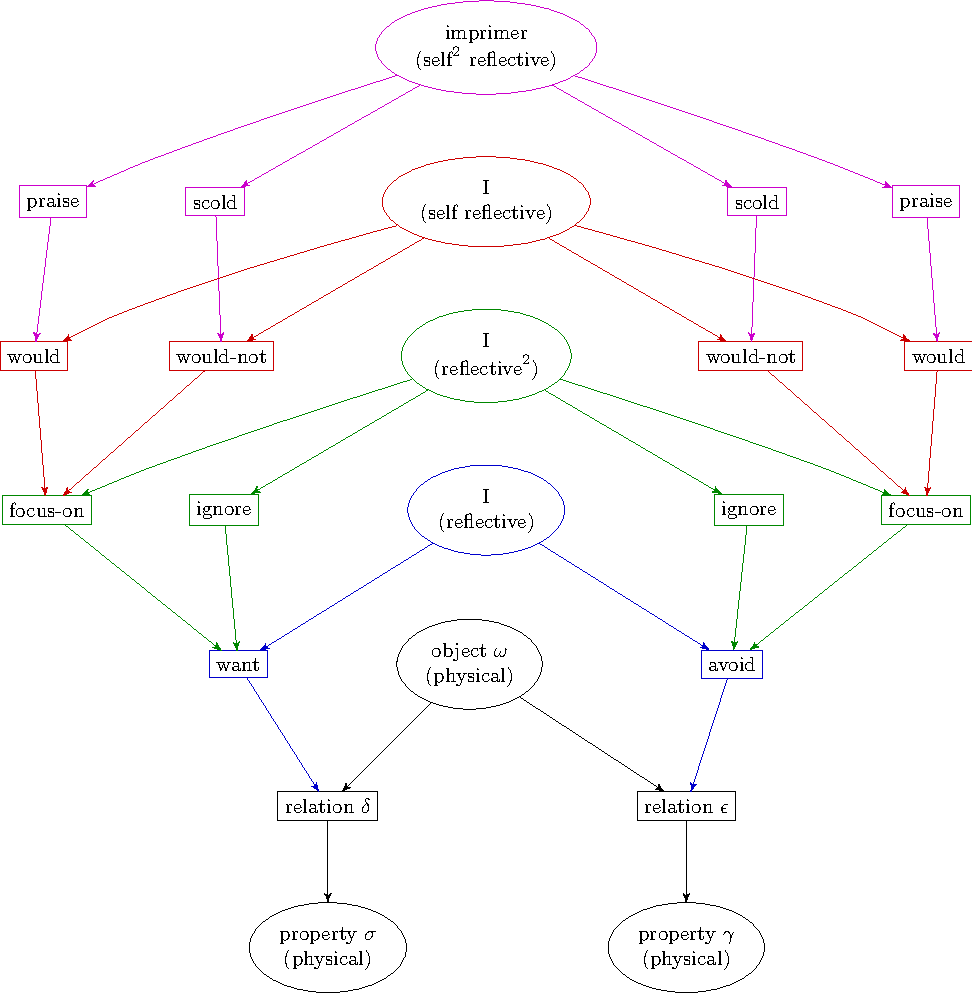
\includegraphics[width=4cm]{gfx/model-6} \\ \medskip

        \myDegree \\ \medskip   
        %\myDepartment \\                            
        %\myFaculty \\
        %\myUni \\ \bigskip

        \myTime

        \vfill                      

    \end{center}  
  \end{addmargin}       
\end{titlepage}   

\mymargins
\thispagestyle{empty}

\hfill

\vfill

\noindent\myName: \textit{\myTitle,} \myDegree, \textcopyright\ \myTime

%\bigskip
%
%\noindent\spacedlowsmallcaps{Supervisors}: \\
%\myProf \\
%\myOtherProf \\ 
%\mySupervisor
%
%\medskip
%
%\noindent\spacedlowsmallcaps{Location}: \\
%\myLocation
%
%\medskip
%
%\noindent\spacedlowsmallcaps{Time Frame}: \\
%\myTime

\mymargins
\cleardoublepage%*******************************************************
% Dedication
%*******************************************************
\thispagestyle{empty}
%\phantomsection 
\refstepcounter{dummy}
\pdfbookmark[1]{Dedication}{Dedication}

\vspace*{3cm}

%\begin{center}
%``If wishes were horses, beggars would ride.''  Since they are not, \\ \medskip
%since really to satisfy an impulse or interest means to work it out, \\ \medskip
%and working it out involves running up against obstacles, \\ \medskip
%becoming acquainted with materials, exercising ingenuity, \\ \medskip
%patience, persistence, alertness, it of necessity involves \\ \medskip
%discipline---ordering of power and supplies knowledge. \\ \medskip
%    --- \defcitealias{dewey:1907}{John Dewey}\citetalias{dewey:1907}
%\end{center}
%
%\medskip

%
%Though there be no such thing as Chance in the world; \\
%our ignorance of the real cause of any event \\
%has the same influence on the understanding, \\
%and begets a like species of belief or opinion.} \\ \medskip
%    --- \defcitealias{hume:1902}{David Hume}\citetalias{hume:1902}
%
%
%

\begin{center}
Though there be no such thing as Chance in the world; \\
our ignorance of the real cause of any event \\
has the same influence on the understanding, \\
and begets a like species of belief or opinion. \\ \medskip
    --- \defcitealias{hume:1902}{David Hume}\citetalias{hume:1902}
\end{center}

\medskip

\begin{center}
    Dedicated to the loving memory of Pushpinder Singh. \\ \smallskip
    1972\,--\,2006
\end{center}

\mymargins
%\cleardoublepage%*******************************************************
% Abstract
%*******************************************************
%\renewcommand{\abstractname}{Abstract}
\pdfbookmark[1]{Abstract}{Abstract}
\begingroup
\let\clearpage\relax
\let\cleardoublepage\relax
\let\cleardoublepage\relax

\chapter*{Abstract}

There have been two directions of research with the goal of building a
machine that explains intelligent human behavior.  The first approach
is to build a baby-machine that learns from scratch to accomplish
goals through interactions with its environment.  The second approach
is to give the machine an abundance of knowledge that represents
correct behavior.

Each of these solutions has benefits and drawbacks.  The baby-machine
approach is good for dealing with novel problems, but these problems
are necessarily simple because complex problems require a lot of
background knowledge.  The data abundance approach deals well with
complicated problems requiring a lot of background knowledge, but
fails to adapt to changing environments, for which the algorithm has
not already been trained.

We are working on an algorithm that benefits from both of these
approaches by learning from cultural language knowledge, while
reflectively monitoring and recognizing the failures of this knowledge
when it is used in a goal-oriented domain.

Toward this end we have developed a reflective programming language
allowing us the ability to monitor the execution and interactions
between large numbers of complicated lisp-like processes.  Further, we
have developed a cognitive architecture within our language that
provides structures for layering reflective processes, resulting in a
hierarchy of control algorithms that respond to failures in the layers
below.

Finally, we present an example of our cognitive architecture learning
in the context of a social commonsense reasoning domain with parents
that teach children as they attempt to accomplish cooking tasks in a
kitchen.

\endgroup

\vfill

%\mymargins
\cleardoublepage%*******************************************************
% Publications
%*******************************************************
\pdfbookmark[1]{Publications}{publications}
\chapter*{Publications}
Some ideas and figures have appeared previously in the following publications:

\bigskip

\noindent Smith, D. and Morgan, B.; "IsisWorld: An open source
 commonsense simulator for AI researchers"; AAAI 2010 Workshop on
 Metacognition; 2010 April

\vspace{5mm}

\noindent Morgan, B.; ``Moral Compass: Commonsense Social Reasoning
 Cognitive Architecture''; http://em-two.net/about; Commonsense Tech
 Note; MIT Media Lab; 2011 January

\vspace{5mm}

\noindent Morgan, B.; ``A Computational Theory of the Communication of
 Problem Solving Knowledge between Parents and Children''; PhD
 Proposal; MIT Media Lab 2010 January

\vspace{5mm}

\noindent Morgan, B.; ``Funk2: A Distributed Processing Language for 
 Reflective Tracing of a Large Critic-Selector Cognitive
 Architecture''; Proceedings of the Metacognition Workshop at the
 Third IEEE International Conference on Self-Adaptive and
 Self-Organizing Systems; San Francisco, California, USA; 2009
 September

\vspace{5mm}

\noindent Morgan, B.; ``Funk2: A Frame-based Programming Language with
 Causally Reflective Capabilities (draft in progress)''; Technical
 Note; Massachusetts Institute of Technology; 2009 May

\vspace{5mm}

\noindent Morgan, B.; ``Learning Commonsense Human-language Descriptions
 from Temporal and Spatial Sensor-network Data''; Masters Thesis;
 Massachusetts Institute of Technology; 2006 August

\vspace{5mm}

\noindent Morgan, B.; ``Learning perception lattices to compare
 generative explanations of human-language stories''; Published
 Online; Commonsense Tech Note; MIT Media Lab; 2006 July

\vspace{5mm}

\noindent Morgan, B. and Singh, P.; ``Elaborating Sensor Data using
 Temporal and Spatial Commonsense Reasoning''; International Workshop
 on Wearable and Implantable Body Sensor Networks (BSN-2006); 2005
 November

\vspace{5mm}

\noindent Morgan, B.; ``Experts think together to solve hard problems'';
 Published Online; Commonsense Tech Note; MIT Media Lab 2005 August

\vspace{5mm}

\noindent Morgan, B.; ``LifeNet Belief Propagation''; Published Online;
 Commonsense Tech Note; MIT Media Lab; 2004 January

\mymargins
\cleardoublepage%*******************************************************
% Acknowledgments
%*******************************************************
\pdfbookmark[1]{Acknowledgments}{acknowledgments}

%Don't do anything that isn't play. \\ \medskip
%    --- Joseph Campbell



\begin{flushright}{\slshape    
Don't do anything that isn't play.} \\ \medskip
    --- Joseph Campbell
\end{flushright}



\bigskip

\begingroup
\let\clearpage\relax
\let\cleardoublepage\relax
\let\cleardoublepage\relax
\chapter*{Acknowledgments}

I would first like to thank:

\begin{itemize}
\item{Push Singh for being a good friend and advisor.}
\end{itemize}

Next I would like to thank my committee:

\begin{itemize}
\item{Joe Paradiso for unfailing support and faith in my ability to do
  something well.}
\item{Marvin Minsky for consistently and patiently providing an
  inspiringly critical perspective and a wealth of important problems
  to solve.}
\item{Gerry Sussman for loving to program.}
\item{Mike Cox for providing critical direction for navigating the
  space of the contemporary meta-cognitive computational sciences.}
\end{itemize}

I would next like to thank my immediate family:

\begin{itemize}
\item{Greg Morgan and Carolyn Spinner for being supportive parents---willing to help me think about anything at any time.}
\item{Paul Bergman for teaching me how to program.}
\item{Virginia Barasch for painting my finger nails.}
\item{Leaf Morgan for playing Archon with me.}
\end{itemize}

Professors:

\begin{itemize}
\item{Henry Lieberman}
\item{Ed Boyden}
\item{Walter Bender}
\item{Ted Selker}
\end{itemize}

Popes:

\begin{itemize}
\item{Dustin Smith}
\item{Scotty Vercoe}
\item{Dane Scalise}
\end{itemize}

Friends:

\begin{itemize}
\item{Mako Hill}
\item{Barbara Barry}
\end{itemize}

\endgroup


\pagestyle{scrheadings}
\mymargins
\cleardoublepage%*******************************************************
% Table of Contents
%*******************************************************
%\phantomsection
\refstepcounter{dummy}
\pdfbookmark[1]{\contentsname}{tableofcontents}
\setcounter{tocdepth}{2} % <-- 2 includes up to subsections in the ToC
\setcounter{secnumdepth}{3} % <-- 3 numbers up to subsubsections
\manualmark
\markboth{\spacedlowsmallcaps{\contentsname}}{\spacedlowsmallcaps{\contentsname}}
\tableofcontents 
\automark[section]{chapter}
\renewcommand{\chaptermark}[1]{\markboth{\spacedlowsmallcaps{#1}}{\spacedlowsmallcaps{#1}}}
\renewcommand{\sectionmark}[1]{\markright{\thesection\enspace\spacedlowsmallcaps{#1}}}%*******************************************************
% List of Figures and of the Tables
%*******************************************************
\clearpage

\begingroup 
    \let\clearpage\relax
    \let\cleardoublepage\relax
    \let\cleardoublepage\relax
    %*******************************************************
    % List of Figures
    %*******************************************************    
    %\phantomsection 
    \refstepcounter{dummy}
    %\addcontentsline{toc}{chapter}{\listfigurename}
    \pdfbookmark[1]{\listfigurename}{lof}
    \listoffigures

    \vspace*{8ex}

    %*******************************************************
    % List of Tables
    %*******************************************************
    %\phantomsection 
    \refstepcounter{dummy}
    %\addcontentsline{toc}{chapter}{\listtablename}
    \pdfbookmark[1]{\listtablename}{lot}
    \listoftables
        
    \vspace*{8ex}
%   \newpage
    
    %*******************************************************
    % List of Listings
    %*******************************************************      
	  %\phantomsection 
    \refstepcounter{dummy}
    %\addcontentsline{toc}{chapter}{\lstlistlistingname}
    \pdfbookmark[1]{\lstlistlistingname}{lol}
    \lstlistoflistings 

    \vspace*{8ex}
       
    %*******************************************************
    % Acronyms
    %*******************************************************
    %\phantomsection 
    \refstepcounter{dummy}
    \pdfbookmark[1]{Acronyms}{acronyms}
    \markboth{\spacedlowsmallcaps{Acronyms}}{\spacedlowsmallcaps{Acronyms}}
    \chapter*{Acronyms}
    \begin{acronym}[UML]
        \acro{GPS}{General Problem Solver}
    \end{acronym}                     
\endgroup

\cleardoublepage

%\cleardoublepage%\manualmark
%\markboth{\spacedlowsmallcaps{Preface}}{\spacedlowsmallcaps{Preface}} % work-around to have small caps also
\refstepcounter{dummy}

%************************************************
\addtocontents{toc}{\protect\vspace{\beforebibskip}} % to have the bib a bit from the rest in the toc
\addcontentsline{toc}{chapter}{\tocEntry{Preface}}
%************************************************

\chapter*{Preface}
\chaptermark{Preface}


%*******************************************************
% Mainmatter
%*******************************************************

%% remarked for starting pages with 1
%\pagenumbering{arabic}


\mymargins
%************************************************
\chapter{Introduction}
\label{chapter:introduction}
%************************************************

An intelligent system thinks about a problem domain, learning the
effects of its actions, constructing and executing plans to accomplish
its goals.  I will refer to these types of thinking about a problem
domain as deliberative thinking.  A reflective intelligence extends
the deliberative intelligence by learning to accomplish goals in its
own deliberative thinking process.  Reflective thinking is sometimes
referred to as ``thinking about thinking'' or ``metacognition.''  A
reflective intelligence can learn to select between different types of
thinking that are appropriate for generating plans toward different
types of goals.  In this thesis, I present the Substrate for
Accountable Layered Systems (SALS), an open-source
\begin{wrapfigure}{r}{6.125cm}
  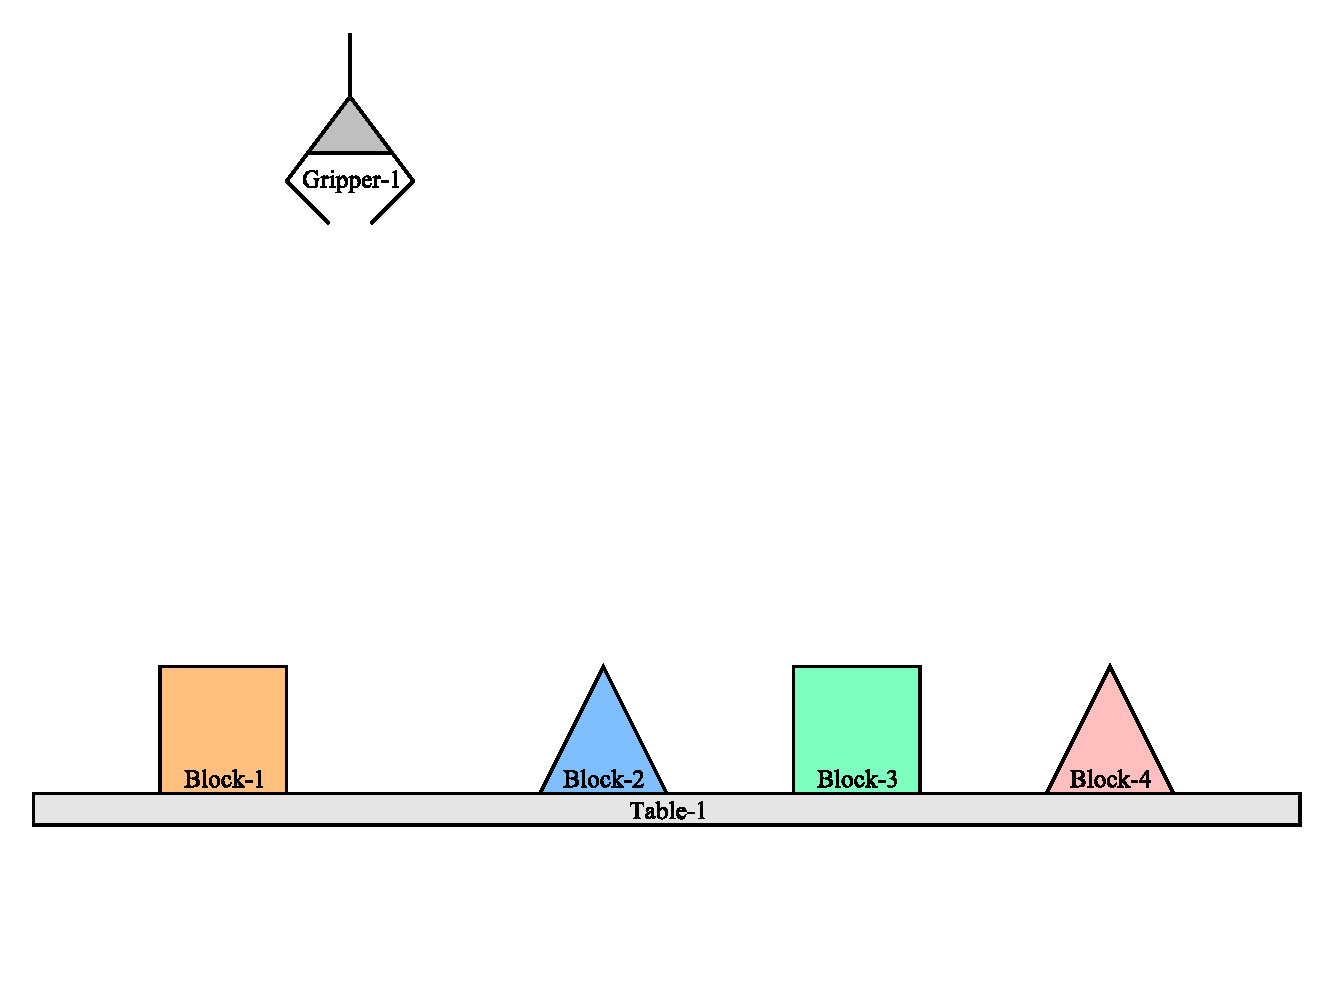
\includegraphics[width=6cm]{gfx/blocks_world_large-01}
  \caption[An example ``Blocks World'' problem domain.]{An example
    ``Blocks World'' problem domain.}
  \label{figure:introduction_example_problem_domain}
\end{wrapfigure}
software platform for the development of experimental reflective
Artificial Intelligences (AI).  A deliberative AI system consists of
three processes: {\mbox{(1)~perceptual}} data are generalized and
categorized to learn abstract models, {\mbox{(2)~abstract}} models are
used to infer hypothetical states, i.e. states of future, past, or
otherwise ``hidden'' variables, {\mbox{(3)~actions}} are chosen based
on considerations of hypothesis dependent inferences.  There are many
approaches to machine learning that focus on this abstract 3-step
closed-loop process of learning to control, such as: reinforcement
learning \cite[]{kaelbling:1996,dvzeroski:2001}, game theory
\cite[]{bowling:2000,rapoport:2001}, and control theory
\cite[]{simon:1982, bertsekas:1995}.  The discipline of computational
metacognition \cite[]{cox_and_raja:2008,cox:2010} focuses on making at
least two layers of closed-loop systems.  Organizing the three-step
architecture within the metacognitive framework, deliberative thinking
is modeled as a closed-loop learning algorithm that perceives and
learns to control the external world, while reflective thinking is
modeled as a second closed-loop learning algorithm that perceives and
learns to control the deliberative thinking process.  While it may be
clear how to trace the inputs to deliberative thinking, there is not a
consensus in the literature on a tractable approach to modeling the
inputs to reflective thinking.  In this thesis, I present a tractable
approach to reflective thinking that implies a scaling to $N$ layers
of reflective control.

\section{Contributions}

The four contributions of this thesis are:
\begin{enumerate}
\item \emph{Emotion Machine Cognitive Architecture}: A computational
  implementation of the bottom four layers of the ``Emotion Machine''
  six-layered theory of mind \cite[]{minsky:2006}.  The implementation
  contains a physical simulation that is controlled by a deliberative
  physical object-level reasoning layer with another reflective
  meta-level reasoning layer that learns to control the deliberative
  problem solving resources.  The architectural primitives include
  resources that are organized into agencies that are organized into
  layers.  The implementation includes five layers that are described
  in
  {\mbox{\autoref{chapter:emotion_machine_cognitive_architecture}}}:
  (1) built-in reactive thinking, (2) learned reacting thinking, (3)
  deliberative thinking, (4) reflective thinking, and (5)
  super-reflective thinking.  The implementation leaves
  self-reflective and self-conscious layers of the Emotion Machine
  theory as future extensions of this research.
\item \emph{Learning from Being Told Natural Language Plans}: A system
  needs a plan library.  Plan libraries can be authored by humans as
  sequences of simple natural language sentences.  The implementation
  includes the ability to interpret and imagine executing natural
  language commands by using analogies to natural language plans that
  it already knows.  In this case, ``being told'' means that a natural
  language plan is programmed into the AI by the user.  Interpreting a
  natural language plan involves parsing the English and generating a
  compiled program, along with imagined hypotheses about the program's
  effects.  These guesses are based on what partial states the plan
  checks for in the control domain as well as rules learned from
  previous executions of similar actions in the past.
\item \emph{Learning Asynchronously from Experience}: Executing plans
  in the external problem domain gives the system better expectations
  for what plans will actually end up doing when they are interpreted
  ({\mbox{\autoref{section:natural_language_plans_interpreting_natural_language_plans}}}),
  imagined
  ({\mbox{\autoref{section:imagining_the_effects_of_ambiguous_natural_language_plans}}})
  and executed
  ({\mbox{\autoref{section:two_experiential_event_streams_flow_to_each_planning_layer}}}).
  I refer to this form of learning the effects of actions in the
  problem domain as learning from ``experience.''  Many types of
  failures can occur when interpreting, imagining and actually
  executing ambiguous natural language plans, such as: expectation
  failures, interpretation failures, type failures, activation
  failures, and a variety of low-level system failures.  These
  experiences of different types of failures inform reflective
  learning algorithms to subsequently predict these types of plan
  failures.  Learning from experience is executed concurrently and
  asynchronously with the currently executing plan.  The learning
  algorithm receives a stream of frame mutation trace events from the
  currently executing plan and uses this stream to learn abstract
  causal rule-based models.  In this way, effects of physical and
  mental actions are learned through experience without slowing down
  the primary plan execution speed.  Such failures are input to the
  reflective layer, which can learn to predict and avoid these
  failures in the future.
\item \emph{Virtual Machine and Programming Language}: A concurrent
  and parallel virtual machine and low-level Lisp-like programming
  language provide the foundation upon which all of the above
  contributions have been implemented.  The virtual machine includes
  native procedural tracing features that facilitate the automatic
  monitoring and control of many concurrently executing tasks.  The
  virtual machine takes advantage of multiple CPU and multiple-core
  CPU hardware configurations.  The programming language is a bytecode
  compiled language and all code for all contributions are open
  source.
\end{enumerate}

\section{A Story of Reflective Learning}

Before getting into abstract generalizations of reflective thinking,
let us consider the advice of Seymour Papert: ``You can't think about
thinking without thinking about thinking about something.''  Following
this advice, consider the simple physical block stacking world,
depicted in {\autoref{figure:introduction_example_problem_domain}},
which is similar to the ``Blocks World'' planning domain
{\cite[]{winograd:1970}}.  Imagine that the robot arm in this simple
scenario is an entirely deliberative (non-reflective) AI that wants to
accomplish the deliberative goal of a block being on a block.  This AI
has the capability of learning both from experience as well as from
being told knowledge.  The deliberative AI has been told a number of
natural language plans for how to pick up and move around blocks in
this problem domain.  What types of thoughts might be going through
the mind of this deliberative block stacking AI?  The following story
might be what this type of deliberative AI would be thinking in this
block stacking domain:
\begin{quote}
  I want to accomplish the deliberative goal of a block being on a
  block.  I must choose how to physically act.  I have a number of
  plans that I have been told, but I don't know what they will do.  I
  am focused on my most recently learned plan for how to physically
  act, which is called, ``stack a cube on a pyramid.''  I have been
  told this plan in natural language, so I must interpret what it
  means if I am going to imagine executing it.  If I can imagine a way
  that this plan could accomplish my deliberative goals, I will
  execute it.  I will try interpreting and imagining the physical
  effects of my most recently learned plan for physical action,
  ``stack a cube on a pyramid.''  I imagine that executing this plan
  will accomplish my goal of a block being on a block.  I will stop
  imagining the rest of my plans and try executing this plan for
  physical action.  I am picking up a cube and dropping it on a
  pyramid.  The cube is falling off of the pyramid and onto the table.
  Oh no!  A block is not on a block.  My expectations have failed!  A
  deliberative plan has failed.  I will relearn the physical effects
  of my physical actions based on this new physical knowledge.  The
  next time that I am dropping a block on a pyramid, I will expect the
  block to fall onto the table.  Now, I must stop executing this plan
  and again choose how to physically act, given my new information.
\end{quote}
In this story, the deliberative AI interprets and imagines executing
plans based on reasoning by natural language analogies.  Because the
deliberative AI experiences a knowledge failure, the deliberative AI
learns a better model of the effects of its physical actions.  If this
AI were reflective, it would be able to learn more from the
deliberative failure of the AI in this story.  A reflective AI not
only learns the effects of physical actions but also learns the
effects of deliberative actions, such as the effects of imagining the
effects of a plan.  How would a reflective AI approach thinking about
accomplishing the same physical goal in the same problem domain?  If
the AI were reflective, the following story might be what it would
think to itself as it tries to reflectively decide how to deliberate
about plans for physical action:
\begin{quote}
  I want to accomplish the deliberative goal of a block being on a
  block.  I also want to avoid my negative reflective goal of keeping
  the deliberative layer from having plans that have failed.  I have
  been told a number of reflective plans for deliberative action, but
  I don't know what they will do.  I must choose a reflective plan for
  deliberative action.  I am focused on my most recently learned
  reflective plan, which is called, ``Find and execute a recently
  learned plan to accomplish my goals.''  I choose to imagine the
  effects of the various possible interpretations of this
  underspecified natural language plan on my deliberative knowledge.
  I can adapt other analogous plans to interpret this one, and I
  imagine that at least one interpretation will not lead to any
  deliberative plans having any execution failures, so I choose to
  execute this reflective plan to ``find and execute a recently
  learned plan to accomplish my goals.''
\end{quote}
At this point in the story, the AI has decided on a plan of
deliberative action.  Notice that this story is very similar to the
first story, except rather than deciding on a plan of physical action,
the reflective planner is deciding on a plan for deliberative action.
In this case, the ``find and execute a recently learned plan to
accomplish my goals'' plan is an implementation of a planning
algorithm within the natural planning language itself.  The fact that
the deliberative planning algorithm is written in the reflective
planning language is one key aspect to the recursive nature of this
approach to reflective learning and control.  The reflective AI has a
number of reflective plans for how to deliberatively plan, the method
that the AI chose in this case tries to find a plan that it has been
told most recently.  So, the AI begins executing this reflective plan,
which becomes the deliberative planning process that tries to find a
plan for acting in the physical problem domain:
\begin{quote}
  I will try interpreting and imagining the physical effects of my
  most recently learned plan for physical action, ``stack a cube on a
  pyramid.''  I imagine that executing this plan will accomplish my
  goal of a block being on a block.  I will stop imagining the rest of
  my plans and try executing this plan for physical action.  I am
  picking up a cube and dropping it on a pyramid.  The cube is falling
  off of the pyramid and onto the table.  A block is not on a block.
  Oh no!  My deliberative expectations have failed!  A deliberative
  plan has failed.  Oh no, I was reflectively trying to avoid
  deliberative plan failures!  My reflective expectations have failed!
  A reflective plan has failed.
\end{quote}
At this point in the story, the AI has encountered two failures that
will lead to two opportunities for learning the effects of both its
physical actions as well as its deliberative actions.  If we consider
what the AI might learn from this story, the AI might think:
\begin{quote}
  I have new support for the hypothesis that dropping a block while
  being over a pyramid leads to two blocks being on the table.  I also
  have new support for the hypothesis that executing plans that try to
  accomplish the goal of a cube being on a pyramid may lead to an
  expectation failure when executed.
\end{quote}
The fact that the AI failed at both the deliberative and reflective
levels allowed the AI to learn two new sets of hypotheses: (1) about
physical actions, and (2) about deliberative actions.  The fact that
more can be learned by adding a reflective layer to a learning
algorithm is inspiration for researching reflective machine learning
in those domains where physically acting is relatively costly while
thinking is relatively cheap.  Now, see how the reflective AI
approaches reflectively thinking differently after it has learned from
this initial experience:
\begin{quote}
  I still want to accomplish the deliberative goal of a block being on
  a block.  I still also want to avoid my negative reflective goal by
  keeping the deliberative layer from having plans that have failed.
  I must choose another reflective plan for deliberative action.  I am
  focused on my most recently learned reflective plan, which is
  called, ``Find and execute a recently learned plan to accomplish my
  goals.''  When I imagine executing this plan, I use my learned
  hypothesis that predicts that executing this reflective plan will
  lead to a failure in the deliberative knowledge.  I choose to not
  execute this plan because it does not avoid my negative reflective
  goal.  I focus on my next plan, ``find and execute an old plan to
  accomplish my goals.''  I can adapt other analogous plans to
  interpret this reflective plan, and I have no hypotheses that
  predict that this plan will lead to any deliberative failures, so I
  choose to execute this reflective plan to ``find and execute an old
  plan to accomplish my goals.''
\end{quote}
After this second round of reflective reasoning, the first reflective
plan is considered and again imagined, but this time the reflective
layer predicts that this reflective plan will lead to a failure in the
deliberative layer because the deliberative conditions are so similar.
For example, executing the same reflective plan in the context of the
same deliberative goals is hypothesized to cause a deliberative
failure.  Because this conflicts with the negative reflective goal to
avoid deliberative failures, the first reflective plan is bypassed.
The AI ends up considering another plan and selecting it for
execution.  The difference between these two plans is in how they
organize their search through possible plans.  The first reflective
plan considers deliberative plans that it has learned most recently,
while the second reflective plan considers deliberative plans that it
has learned furthest in the past.  In general, plans may be
reflectively organized in more complicated mental structures, but in
order to simply demonstrate my point, plans are organized in a
doubly-linked list structure that goes forward and backward in time.
One could imagine organizing plans by location, goal, or other equally
important metrics in more complex data structures.  Now that the AI
has reflectively chosen a different way to deliberatively plan, the AI
executes this reflective plan, which becomes the deliberative
reasoning process:
\begin{quote}
  I will try interpreting and imagining the physical effects of my
  oldest plan for physical action, ``stack a pyramid on a cube.''  I
  imagine that executing this plan will accomplish my goal of a block
  being on a block.  I will stop imagining the rest of my plans and
  try executing this plan for physical action.  I am picking up a
  pyramid and dropping it on a cube.  The pyramid is now sitting on
  the cube.  A block is on a block.  Yay!  Executing my oldest plan
  for physical action has accomplished my deliberative goal!  Yay!  I
  have also avoided my negative reflective goal to avoid deliberative
  plan failures!
\end{quote}
So, finally, the reflective AI is happy to accomplish its deliberative
goal.  Note that the deliberative algorithm would have eventually
found and executed the correct deliberative plan, if it had gone
through all of its plans and imagined all of their effects, finally
getting to its oldest plan, which happened to be the successful one.
The advantage of the reflective learning algorithm is that it allows
learning different ways of planning for dealing with different types
of deliberative goals.  Reflective planning allows learning how
different plan representations, planning algorithms, and other
deliberative knowledge is relevant to creating plans toward different
types of deliberative goals.

\section{Layers of Knowledge}

One tricky aspect of programming reflective learning algorithms is
keeping clear distinctions between different layers of knowledge in
the AI.  {\autoref{table:physical_deliberative_reflective_knowledge}}
shows a few examples of physical, deliberative and reflective
knowledge.
\begin{table}
\centering
\begin{tabular}{|p{2cm}|p{8cm}|}
\hline \emph{Physical Knowledge} & \begin{packed_itemize}
\item{A cube is on a pyramid.}
\item{A gripper is moving left.}
\item{A gripper is above a cube.}
\item{A cube is to the left of a pyramid.}
\end{packed_itemize} \\
\hline \emph{Deliberative Knowledge} & \begin{packed_itemize}
\item{Goal 1 is for a cube to be on a pyramid.}
\item{Plan 1 is to stack a pyramid on a cube.}
\item{Plan 1 fails for Goal 1.}
\item{Goal 2 is for a pyramid to be on a cube.}
\item{Plan 1 succeeds for Goal 2.}
%% \item{A deliberative planner has the goal for a cube to be on a
%%   pyramid.}
%% \item{A deliberative planner is focusing on a deliberative plan that
%%   has failed in execution.}
%% \item{The next deliberative plan has not been imagined.}
%% \item{A deliberative planner is focusing on a deliberative plan that
%%   is hypothesized to cause a cube to be on a pyramid.}
\end{packed_itemize} \\
\hline \emph{Reflective Knowledge}   & \begin{packed_itemize}
\item{Goal 3 is to avoid a deliberative planner being focused on a
  deliberative plan that has failed in execution.}
\item{Plan 2 is to find a recent plan to acheive one of my positive
  goals.}
\item{Plan 2 fails for Goal 3.}
\item{Plan 3 is to find an old plan to acheive one of my positive
  goals.}
\item{Plan 3 did not fail for Goal 3.}
%% \item{A reflective planner is focusing on a reflective plan that has
%%   failed in execution.}
%% \item{A reflective planner has the negative goal to avoid a
%%   deliberative planner being focused on a deliberative plan that has
%%   failed in execution.}
%% \item{The next reflective plan has not been imagined.}
%% \item{A reflective planner has the reflective goal for a deliberative
%%   planner to be focusing on a deliberative plan that is hypothesized
%%   to cause a cube to on a pyramid.}
\end{packed_itemize} \\
\hline
\end{tabular}
\caption{Examples of physical, deliberative and reflective knowledge.}
\label{table:physical_deliberative_reflective_knowledge}
\end{table}
Note that there is a strict hierarchy in the knowledge references
between these layers.  Physical knowledge cannot reference knowledge
in other layers.  An example of physical knowledge is: ``a pyramid is
on a cube.''  Physical knowledge is the representation of the problem
domain.  Deliberative knowledge cannot reference reflective knowledge
but can reference physical knowledge.  An example of deliberative
knowledge is: ``a deliberative planner has the goal for a cube to be
on a pyramid.''  Deliberative knowledge includes positive and negative
goals that specify which partial states of the physical knowledge
should be sought or avoided.  In addition to goals, deliberative
knowledge includes plans, a planner, and potentially failures as well.
Reflective knowledge can reference deliberative knowledge, which
allows indirect reference to some deliberatively referenced physical
knowledge as well.  An example of reflective knowledge is: ``A
reflective planner has the reflective goal for a deliberative planner
to be focusing on a deliberative plan that is hypothesized to cause a
cube to be on a pyramid.''  Reflective knowledge is analogous to
deliberative knowledge, but instead of being about accomplishing goals
in physical knowledge, reflective knowledge is about accomplishing
goals in deliberative knowledge.
{\autoref{figure:three_knowledge_layers}} shows the hierarchical
relationship between the physical, deliberative and reflective
knowledge layers in SALS.  In general, one can imagine that the
recursive nature of SALS allows for any number of reflective layers to
be added to the top of the reflective AI, resulting in
``super-reflective'' layers of learning planned control.
\begin{figure}
  \center
  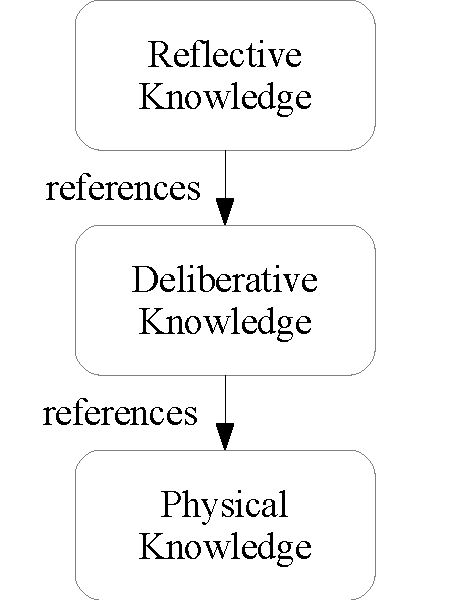
\includegraphics[width=4cm]{gfx/three_knowledge_layers}
  \caption{Three knowledge layers.}
  \label{figure:three_knowledge_layers}
\end{figure}

\section{Natural Language Plans}

SALS includes a simple but powerful planning language that is based on
the interpretation of natural language plans.  Plans are sequences of
commands that can be created, mutated, and executed by a planner in
order to accomplish goals.  The following is an example of a
definition of one of the deliberative plans that the AI in the story
could consider executing:
\begin{samepage}
\begin{Verbatim}
[defplan 'move slowly until over a cube'
  [plan-call [plan 'if a cube is to my left, move slowly
                    left until over a cube, otherwise if a
                    cube is to my right, move slowly right
                    until over a cube']]
  [plan-call [plan 'assert that a cube is below me']]]
\end{Verbatim}
\end{samepage}
This expression defines a new deliberative plan.  The ``defplan''
command is shorthand for ``define plan.''  The first argument to the
defplan expression is the name of the plan: ``move slowly until over a
cube.''  The body of the plan is the remaining sequence of
expressions.  The first expression in the body of this plan is to
interpret and execute the natural language phrase beginning with ``if
a cube...''  The second expression in the body of this plan is to
interpret and execute the natural language phrase beginning with
``assert that...''  This plan positions the AI over a cube and fails
if a cube is not finally below the AI.  If the planner wanted to find
a plan to position the AI over a pyramid, this plan would not help
unless it was slightly modified, replacing all mentions of ``cube''
with ``pyramid.''  In order to help the planner to know what parts of
plans might be analogously replaceable in this way, the SALS planning
language includes optional natural language pattern matching templates
and default frame variable bindings that can be specified for each
plan definition.  The following example shows how this simple plan can
be generalized to allow positioning the AI over a range of shapes:
\begin{samepage}
\begin{Verbatim}
[defplan 'move slowly until over a cube'
  :matches ['move slowly until over a [? shape]']
   :frame [[shape 'cube']]
    [plan-call [plan 'if a [? shape] is to my left, move
                      slowly left until over a [? shape],
                      otherwise if a [? shape] is to my
                      right, move slowly right until over
                      a [? shape]']]
    [plan-call [plan 'assert that a [? shape] is below me']]]
\end{Verbatim}
\end{samepage}
This generalized form of the original plan uses natural language
variables that are specified with a question mark expression, ``?''
Note that there are two optional arguments to the defplan expression
in this example: (1) ``:matches'' and (2) ``:frame.''  The optional
``:matches'' argument specifies a list of potential patterns that this
plan may match as it is being interpreted.  In this case, the variable
expression ``[? shape]'' is allowed to replace the word ``cube'' from
the original name of the plan.  The optional ``:frame'' argument
specifies the default natural language variable bindings.  In this
case, the ``shape'' variable is assigned the natural language phrase
``cube'' by default.  In the body of the generalized form of the plan,
all occurrences of cube have been replaced with the variable
expression ``[? shape]''.  Given this generalized form of the original
plan, the planner can create a new analogous plan as an interpretation
of the natural language phrase ``move slowly until over a pyramid.''
In this way, plans can be communicated to the AI in a natural language
form.  The AI has ``been told'' a total of approximately seventy
simple natural language plans, which can be adapted by analogy to
provide interpretations for a variety of complex possible natural
language plans, including recursive interpretations.  The details of
the planning language will be discussed in
{\mbox{\autoref{chapter:learning_from_being_told_natural_language_plans}}}.

\section{Layers of Learning}

SALS includes an efficient relational learning algorithm in each layer
of planned thinking.  Relational learning in SALS is handled
concurrently with the plan execution in that layer.  In this way, as
plans are executed at full speed, a trace of changes are produced and
sent to a parallel event consuming algorithm that induces abstract
partial states that are used to train a rule learning algorithm.  The
hypotheses that the rule learning algorithm creates are used to
provide explanations as to the parts of the plan that have caused the
traced changes.  I have found that the separation of learning and
planning into concurrent algorithms gives the learning algorithm the
time to work more slowly, while the plan execution can be performed in
bursts at near full speed.

The deliberative layer makes deliberative plans composed of physical
actions in order to accomplish deliberative goals, while the
reflective layer makes reflective plans composed of deliberative
actions in order to accomplish reflective goals.  Deliberative
learning allows the AI to better predict the physical effects of
deliberative plans for physical action, while reflective learning
allows the AI to better predict the deliberative effects of reflective
plans for deliberative action.  The AI is learning at a reflective
level when it thinks to itself, ``I also have new support for the
hypothesis that executing plans that try to accomplish the goal of a
cube being on a pyramid may lead to an expectation failure when
executed.''  This newly supported hypothesis is a reflective
hypothesis about deliberative actions and objects.  The AI
hierarchically assigns credit to the responsible parts of the
executing plan, ``find and execute a recently learned plan to
accomplish my goals,'' that was currently executing at the time of the
unexpected failure.  This precondition for the execution of the plan
is hypothesized to lead to the effects of this action in deliberative
knowledge, ``a deliberative planner is focused on a plan that has
failed.''  The next time that the reflective layer is deciding whether
or not the deliberative planner should execute a given plan, it can
consider this new knowledge and predict whether or not executing the
current plan will put the deliberative planner into a negative or
positive deliberative goal state.  I will discuss the details of SALS'
parallel relational learning algorithm in
{\mbox{\autoref{chapter:learning_asynchronously_from_experience}}}.

\section{Document Overview}

Each of the four contributions of this thesis will be discussed in one
of the following four chapters.  My implementation of the bottom four
layers of an Emotion Machine cognitive architecture is discussed next
in {\mbox{\autoref{chapter:emotion_machine_cognitive_architecture}}}.
In
{\mbox{\autoref{chapter:learning_from_being_told_natural_language_plans}}},
I will describe the natural language planning language that allows
natural language plans to ``be told'' to the AI.  This chapter will
also discuss how the planning process interprets natural language
plans by finding analogies to plans that the AI already knows.  In
{\mbox{\autoref{chapter:learning_asynchronously_from_experience}}}, I
will describe how the AI learns from the experience it gains from
actually executing its plans.  This chapter will describe the
necessary procedurally reflective components that have been used to
attach complex time-intensive learning algorithms to quickly executing
plans of action.  In order to describe my last contribution, I will
describe the SALS virtual machine and reflectively traced programming
language in
{\mbox{\autoref{chapter:virtual_machine_and_programming_language}}}.

{\mbox{\autoref{chapter:related_models}}} relates my AI to other
contemporary cognitive architectures, approaches to reflective
thinking, metacognition, and learning to plan, as well as other
massively multithreaded computer systems.
{\mbox{\autoref{chapter:evaluation}}} evaluates the run-time
performance of the SALS AI and shows a sub-linear increase in
time-complexity for each additional reflective layer.  In
{\mbox{\autoref{chapter:future}}}, I discuss promising directions of
future research for extending this architecture to learn at the top
two layers of the Emotion Machine theory, the self-reflective and
self-conscious layers.  Also, in this chapter I discuss approaches to
overcoming some of the current limitations in the SALS cognitive
architecture.



\mymargins
\cleardoublepage\part{Contributions}\label{part:contributions}
\mymargins
\chapter{Emotion Machine Cognitive Architecture}
\label{chapter:emotion_machine_cognitive_architecture}

The SALS cognitive architecture is inspired by the bottom four layers
of the {\emph{Emotion Machine}} theory of human commonsense thinking
described by \cite{minsky:2006}.  SALS includes architectural
primitives for defining different types of reflective AIs.  The most
basic component of the SALS architecture is an object called a
{\emph{resource}}.  In general, a resource is any compiled procedure
that can be executed by activating the resource.  A resource is said
to be {\emph{activated}} if it is currently executing.  A resource may
be activated as an action in a plan.  If a resource is currently
executing, a {\emph{duplicate activation failure}} results from an
attempted additional activation of the resource.  If a resource is not
currently activated, a resource may be {\emph{suppressed}}, which is a
logical internal state of the resource that causes any attempts to
activate the resource to result in a {\emph{suppressed activation
    failure}}.  Resources are usually assigned simple functions that
do not do complicated or intelligent reasoning tasks themselves, but
instead, resources are generally designed so that they perform
primitive activities that can be combined in various ways to perform
various resultingly complex tasks.  For example, the simplest
resources in the SALS AI that interact directly with the physical
simulation do simple tasks like: ``{\tt{start moving left}},''
``{\tt{start moving right}},'' ``{\tt{stop moving}},''
``{\tt{reach}},'' and ``{\tt{grab}}.''  Resources may be activated or
suppressed by plans in the layer above those resources.  If a resource
is suppressed and activated at the same time, this results in an
activation failure that causes a plan to stop executing, so that it
may be reflectively debugged at a higher layer.  Some resources in
SALS are referred to as {\emph{vital resources}} because they are
activated when the AI is initially created and they never complete
execution.  For example, one vital resource monitors any changes to a
visual knowledge base and attempts to create a stable physical model
of the world from these changes.  Vital resources are usually used for
processing streams of reflective trace events that monitor and learn
from the effects of other executing resources.

Resources are grouped into collections called {\emph{agencies}}.
Agencies tend to be used for combining resources that are used for
accomplishing similar types of goals.  For example, the low-level
resources that control the physical simulation are referred to as a
{\emph{physical agency}}.  Resources that can be activated and used
for solving problems are usually grouped into agencies that separate
them from the vital resources.  For example, the vital resources that
process low-level visual knowledge trace events are separated into a
{\emph{sensory agency}}.

Agencies are further grouped into collections called {\emph{layers}}.
The SALS AI consists of five layers of reflective control.  These
layers are:
\begin{samepage}
  \begin{packed_enumerate}
  \item{{\emph{The Built-In Reactive Layer}}}
  \item{{\emph{The Learned Reactive Layer}}}
  \item{{\emph{The Deliberative Layer}}}
  \item{{\emph{The Reflective Layer}}}
  \item{{\emph{The Super-Reflective Layer}}}
  \end{packed_enumerate}
\end{samepage}
{\mbox{\autoref{figure:five_layers_overview}}} shows an overview of
the five layers of the reflective AI.
\begin{figure}
\centering
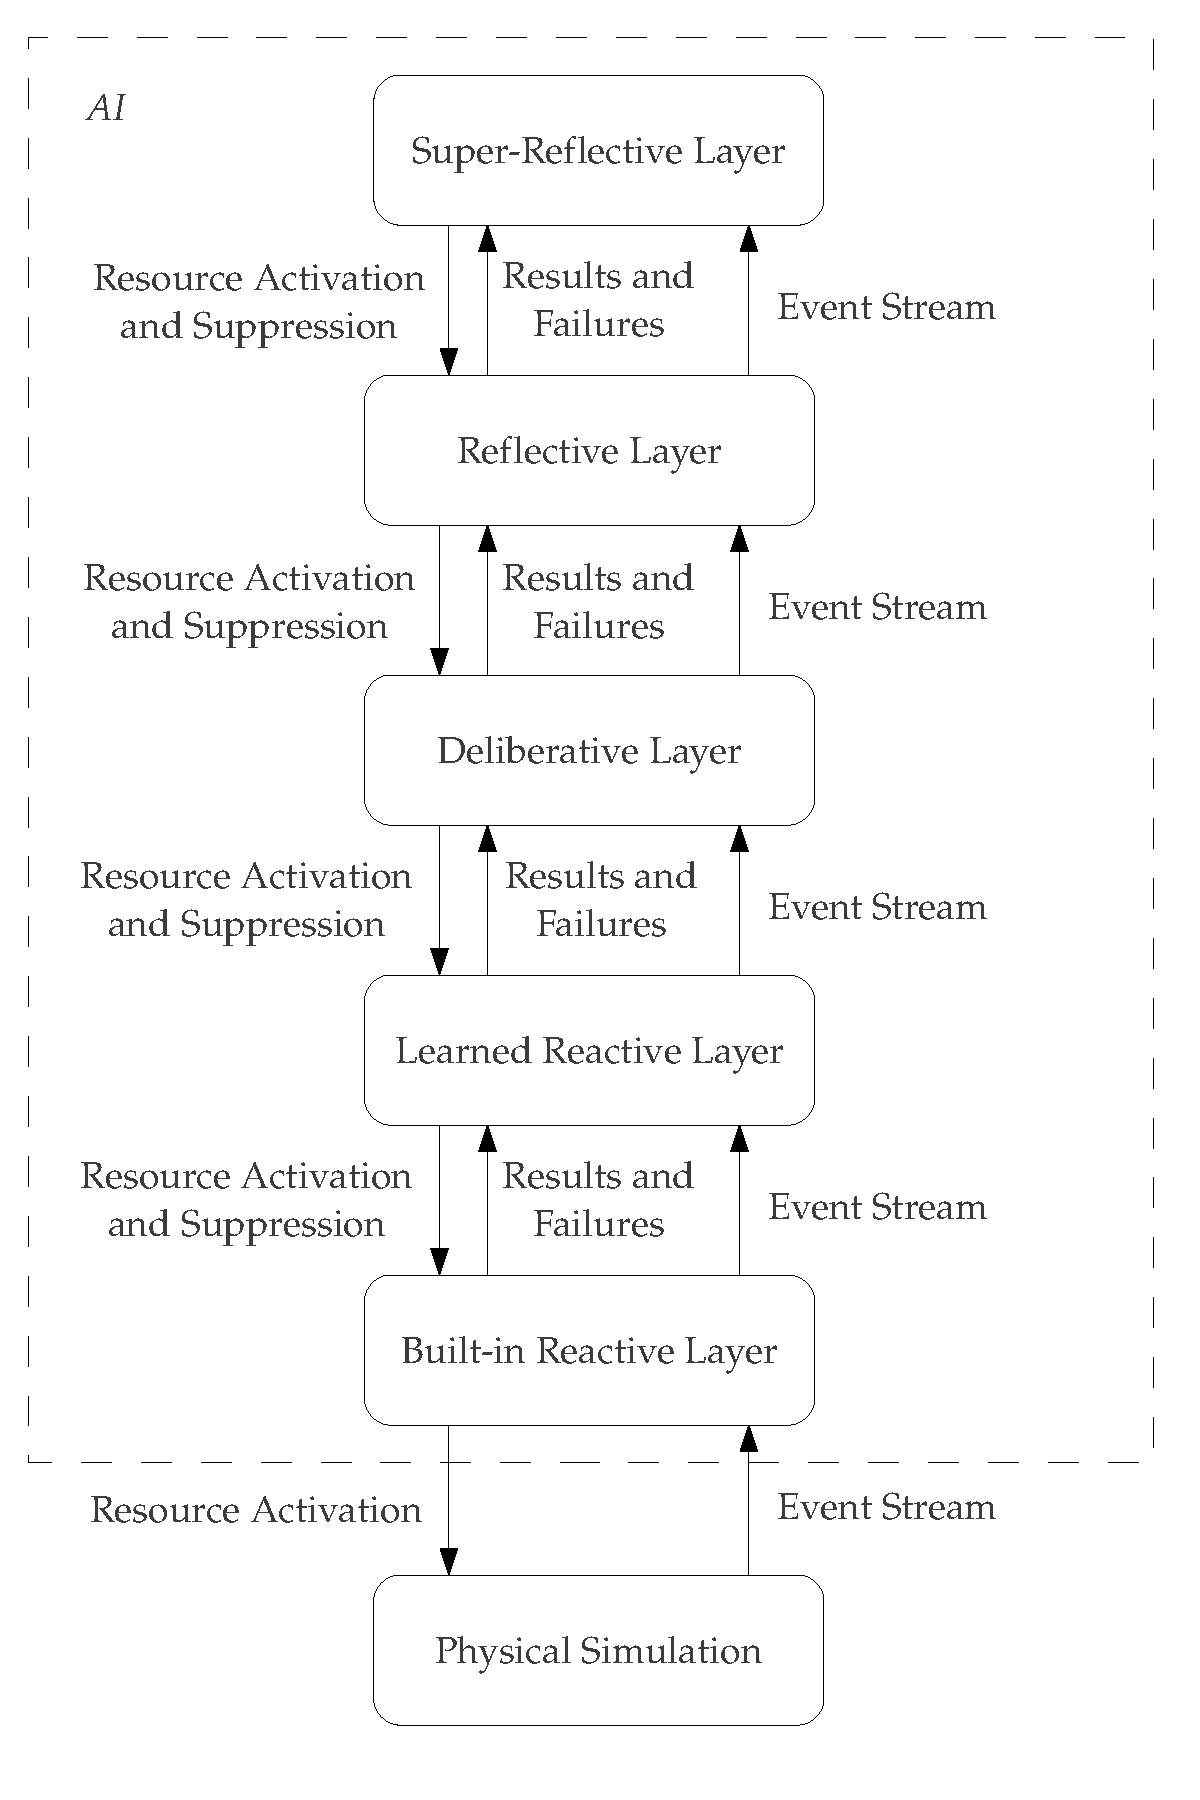
\includegraphics[width=10cm]{gfx/five_layers_overview}
\caption[The five layers of the AI in relation to the physical
  simulation.]{The five layers of the AI in relation to the physical
  simulation.}
\label{figure:five_layers_overview}
\end{figure}
The layers of the AI form cascaded control loops, where each layer
controls the layer below.  One would expect that in a real human there
are cases where lower layers activate and suppress upper layers, such
as hunger suppressing rational deliberation.  In SALS, this is
implemented as a reflective process that executes a deliberative plan
that periodically checks a specific negative physical goal state
exists and fails if it does, which would cause the reflective process
to suppress the appropriate deliberative resources.

\section{The Physical Simulation}

The physical simulation that is used to demonstrate the SALS AI,
depicted in
{\autoref{figure:introduction_example_problem_domain__duplicate_1}},
is similar to the {\emph{Blocks World}} planning domain
\begin{wrapfigure}{r}{6.125cm}
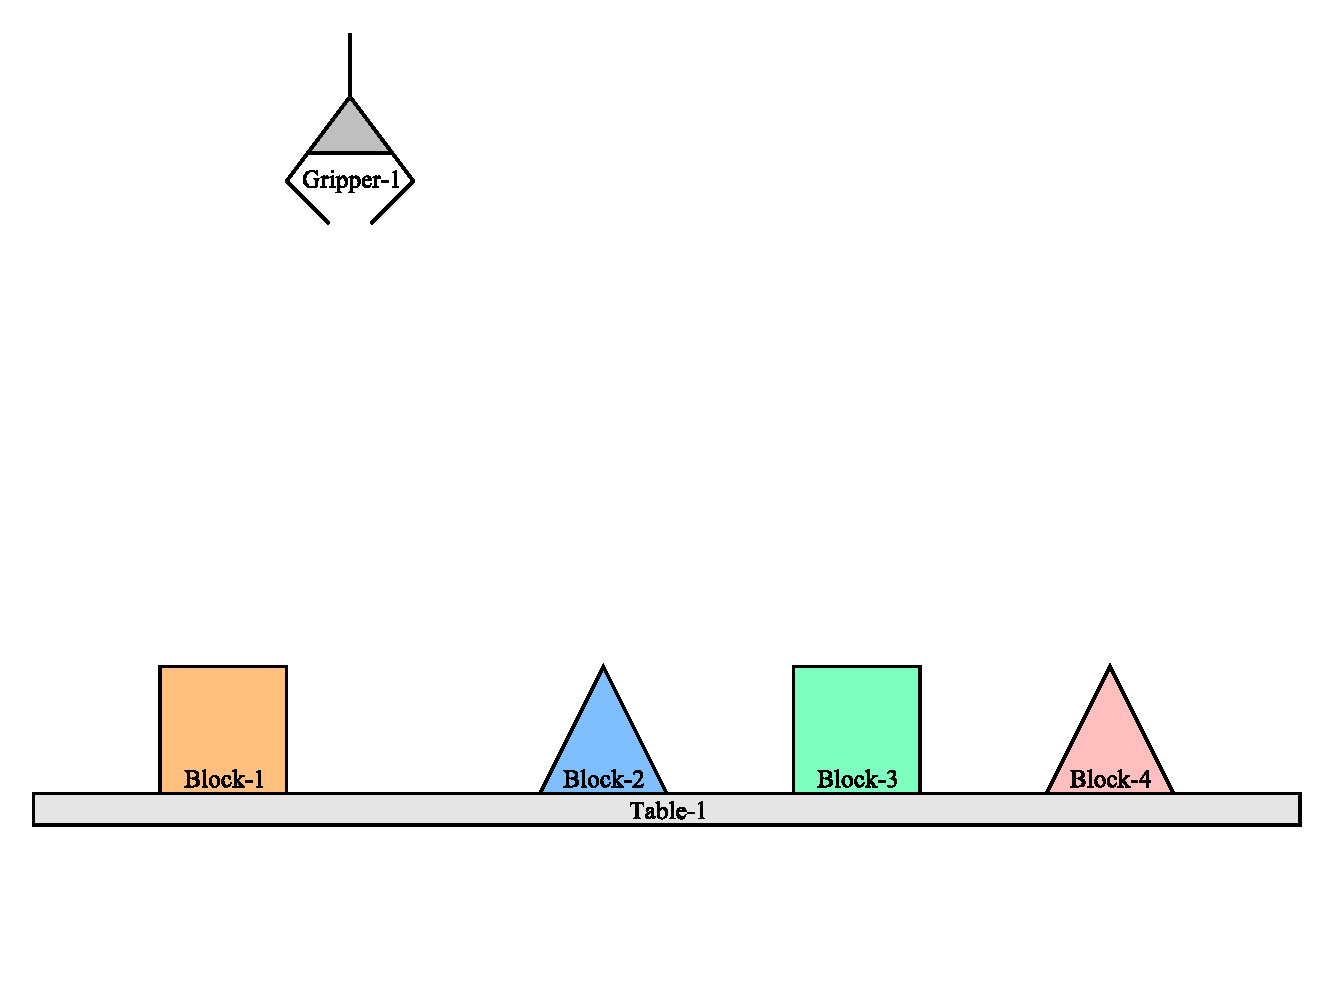
\includegraphics[width=6cm]{gfx/blocks_world_large-01}
  \caption[An example {\emph{Blocks World}} problem domain.]{An
    example {\emph{Blocks World}} problem domain, duplicated from
    {\mbox{\autoref{figure:introduction_example_problem_domain}}}.}
  \label{figure:introduction_example_problem_domain__duplicate_1}
\end{wrapfigure}
{\cite[]{winograd:1970}}.  The physical simulation is a 2-dimensional,
deterministic, rigid-body physical simulation based upon a
floating-point implementation of Newtonian physics ($F=ma$).  The
simulation is stepped with a time step of $0.1$ seconds.  The gripper
can be controlled by the SALS AI to move left or right at one of two
different speeds, fast ($1\text{ m}/\text{s}$) or slow ($0.25\text{
  m}/\text{s}$).  The simulation is meant to be a model of a
continuous-time domain, rather than the logical propositional type of
domain that is often used in other Blocks World simulations.  The
dexterous manipulation problem of the gripper picking up a block is
simplified by simply allowing the gripper to magically grab a block
when it touches the top of the block.  When a square block is dropped
on top of a triangular block, the square block will fall to the table
in the direction of the center of mass of the square relative to the
triangle.  The physical simulation is programmed to recognize spatial
relationships between objects, such as ``{\tt{left-of}},''
``{\tt{below}},'' and ``{\tt{inside-of}}.''  As the physical
simulation is stepped, the SALS AI receives a stream of relationship
changes from the physical simulation.

\section{The Built-In Reactive Layer}

The built-in reactive layer is the layer of the AI that connects to
the problem domain.  In the example, the problem domain is a physical
block stacking world.  The lowest level action and perception agencies
are in the built-in reactive layer, such as physical and sensory
agencies.  The built-in reactive physical agency contains resources
that send asynchronous commands to the physical simulation, which
means that these resources do not receive any response from the
physical world, and thus do not report any types of failure or success
status messages after they have completed being activated.  The
built-in reactive physical resources are for the primitive actions of
the physical simulation.  The primitive actions that are exported by
the physical simulation directly change its state.  For example, the
resource, ``{\tt{start moving left}},'' can be thought of as applying
5 volts to a DC motor.  The motor may or may not start turning, but
the application of the voltage cannot be sensed as a failure.  The
``{\tt{start moving left}}'' built-in reactive resource puts the
physical simulation into the state of trying to move left.  There is
no way that this very basic state changing function can fail in this
sense.  Any failure to actually move the robot arm to the left must be
detected as an expectation failure at a higher level of reasoning that
correlates actions with changes in sensory perceptions.  The built-in
reactive sensory agency receives a stream of change events from the
state of the physical simulation.  A {\emph{change event}} is a
frame\footnote{\emph{frame}: A frame is a memory object that contains
  attribute or property values \cite[]{minsky:1975}.  Attributes of
  frames can be frames themselves, allowing for the definition of
  recursive memories.} that consists of a removed attribute or
property to or from a given frame object at a given time.  Details of
change events will be discussed in
{\mbox{\autoref{chapter:learning_asynchronously_from_experience}}},
{\mbox{\autoref{section:partial_state_event_abstraction}}}.  From this
stream of changes, a visual knowledge base is constructed in the
built-in reactive layer.

\subsection{The Visual Knowledge Base}

Knowledge bases in SALS consist of collections of interconnected
frame-based objects.  The visual knowledge base consists of visual
objects that have a number of property slots with different sets of
possible symbolic values:
\begin{samepage}
  \begin{packed_itemize}
  \item{{\emph{type}}: $\{$``{\tt{block}}'', ``{\tt{table}}'', ``{\tt{gripper}}''$\}$}
  \item{{\emph{shape}}: $\{$``{\tt{cube}}'', ``{\tt{pyramid}}''$\}$}
  \item{{\emph{color}}: $\{$``{\tt{red}}'', ``{\tt{green}}'', ``{\tt{blue}}'', ``{\tt{brown}}'', ``{\tt{white}}'', ``{\tt{black}}''$\}$}
  \item{{\emph{movement-command}}: $\{$``{\tt{move-left}}'', ``{\tt{move-right}}'', ``{\tt{move-left-slowly}}'', ``{\tt{move-right-slowly}}'', ``{\tt{stop}}'', ``{\tt{reach}}'', ``{\tt{grab}}'', ``{\tt{recoil}}''$\}$}
  \end{packed_itemize}
\end{samepage}
These properties are meant to be those aspects of the physical world
that the AI can see about a single object, including the type, shape
and color of a visual object.  Also, the AI can see what the robot
arm, or ``{\tt{gripper}}'', is currently commanded to do.  The current
activity of a gripper object is stored in the
``{\tt{movement-command}}'' property slot.  In addition to each visual
object having properties, each visual object may have different types
of relations to other visual objects that the AI can currently see.

\begin{samepage}
  \begin{packed_itemize}
  \item{\tt{on}}
  \item{\tt{above}}
  \item{\tt{below}}
  \item{\tt{right-of}}
  \item{\tt{left-of}}
  \item{\tt{below-right-of}}
  \item{\tt{below-left-of}}
  \item{\tt{inside-of}}
  \end{packed_itemize}
\end{samepage}

\begin{figure}
\centering
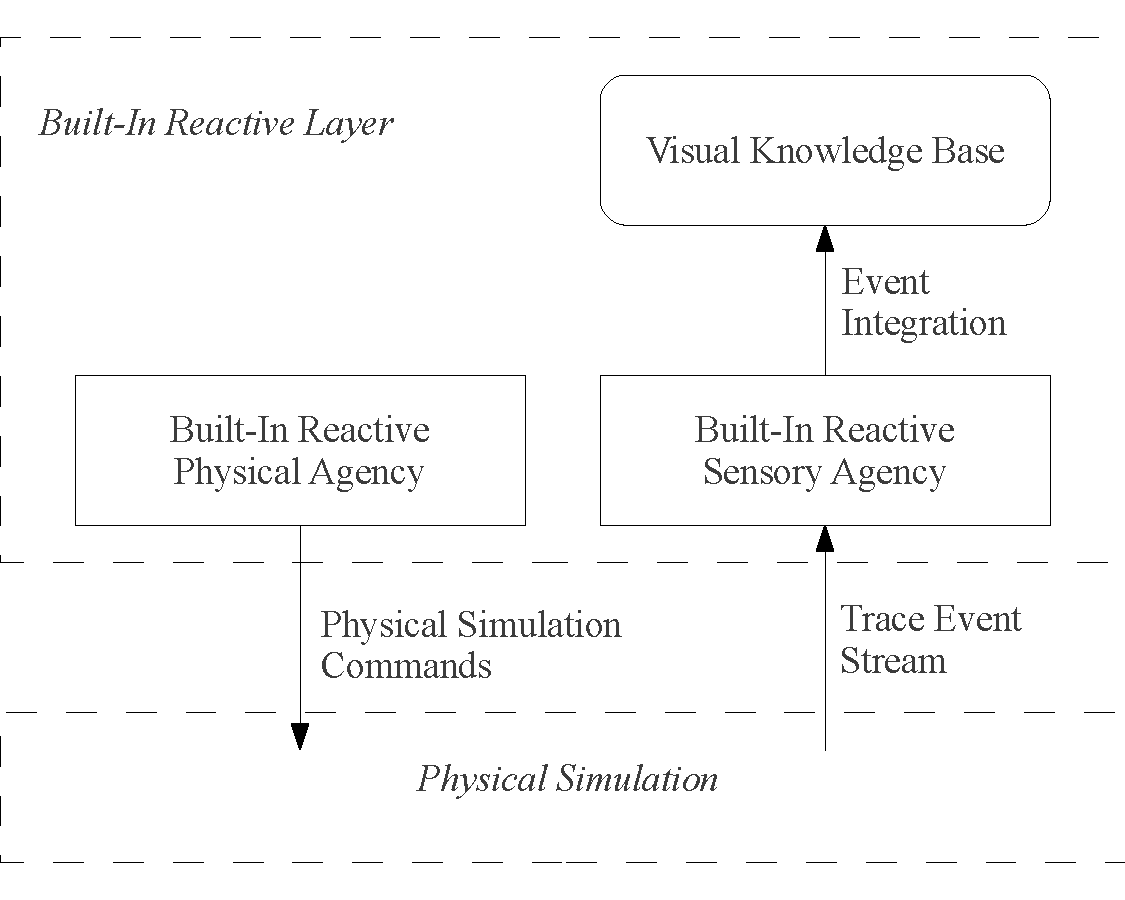
\includegraphics[width=10cm]{gfx/built_in_reactive_and_physical_layers}
\caption{The built-in reactive layer communicates with the physical
  simulation.}
\label{figure:built_in_reactive_and_physical_layers}
\end{figure}
As can be seen in
{\mbox{\autoref{figure:built_in_reactive_and_physical_layers}}}, the
built-in reactive physical and sensory agencies connect the AI to the
physical simulation.  Also shown is the visual knowledge base, the
initial sensory knowledge base in the AI.

\section{The Learned Reactive Layer}

The learned reactive layer in SALS does not have direct access to the
physical simulation.  Instead, the learned reactive layer perceives
the visual knowledge base in the built-in reactive layer and sends
activation or suppression commands to the built-in reactive physical
agency resources.  The learned reactive layer is similar to the
built-in reactive layer because it also contains a {\emph{physical
    agency}}.  However, the learned reactive physical agency contains
resources that execute compiled plans from the deliberative layer
above.  When these resources are activated, they execute plans that
contain sequences of commands that end up either activating or
suppressing built-in reactive resources in the layer below.  Learned
reactive physical resources can fail for a variety of reasons that
will be introduced later when I present the details of plans and the
planning process in
{\mbox{\autoref{chapter:learning_from_being_told}}}.

\subsection{The Physical Knowledge Base}

The learned reactive layer contains an agency called the
{\emph{physical knowledge agency}}.  The physical knowledge agency
contains resources that receive a trace event stream of any changes in
the visual knowledge base.  In partially observable environments, the
physical knowledge base contains a representations of the physical
world that is larger than the current visual knowledge base may
contain as direct sensory knowledge.  The block stacking domain is not
a partially observable environment, so the physical knowledge base in
this case is simply a reconstructed copy of the visual knowledge base.
However, in IsisWorld {\cite[]{smith:2010}}, the partially observable
physical problem domain,
% shown in
%{\mbox{\autoref{figure:isis_world_two_agents_labelled}}},
SALS utilizes the distinction between visual and physical knowledge as
the physical knowledge base is larger than the partial view of
knowledge provided by the visual knowledge base.  In this
dissertation, I will not describe the larger number of different types
of objects with more complex relationships and properties that occur
in the IsisWorld physical simulation.  Because my focus is on learning
to plan and learning to reflectively plan, the visual and physical
details of the IsisWorld simulation would only confuse my point.
%\begin{figure}
%\centering
%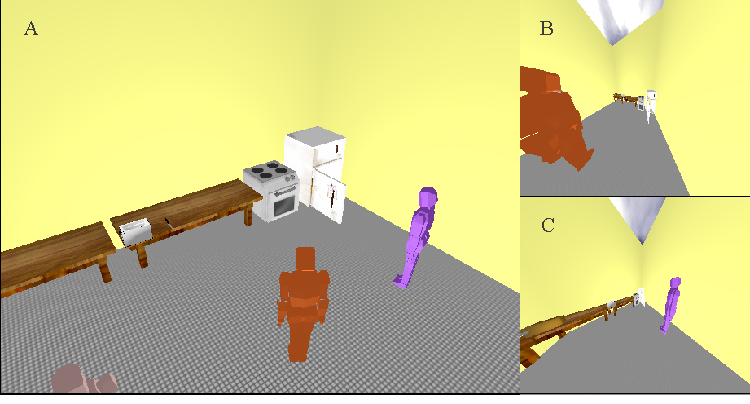
\includegraphics[width=12cm]{gfx/isis_world_two_agents_labelled}
%\caption[IsisWorld physical simulation with two humanoid robots in a
%  partially observable physical problem domain.]{IsisWorld physical
%  simulation with two humanoid robots in a partially observable
%  physical problem domain.  (A) An overview of the entire physical
%  simulation from an omniscient perspective.  (B, C) Each robot only
%  sees a partial perspective of the entire physical domain, depending
%  on each robot's visual perspective.}
%\label{figure:isis_world_two_agents_labelled}
%\end{figure}

\begin{figure}
\centering
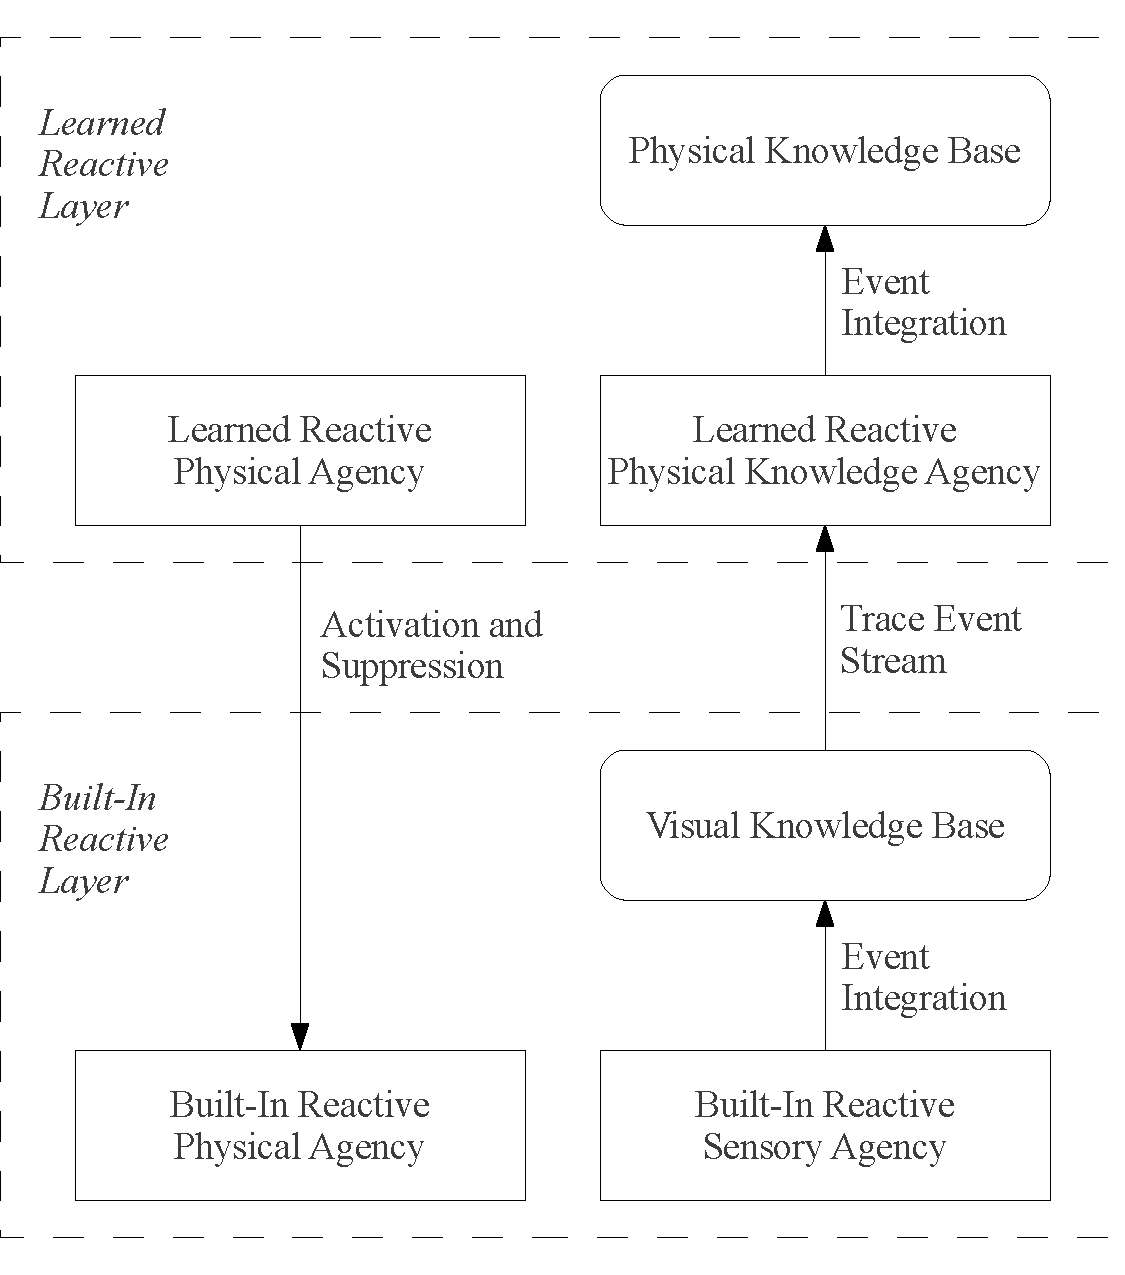
\includegraphics[width=10cm]{gfx/learned_reactive_and_built_in_reactive_layers}
\caption{The learned reactive layer communicates with the built-in
  reactive layer.}
\label{figure:learned_reactive_and_built_in_reactive_layers}
\end{figure}
As can be seen in
{\mbox{\autoref{figure:learned_reactive_and_built_in_reactive_layers}}},
the learned reactive physical and physical knowledge agencies connect
the higher layers of the AI to the built-in reactive layer.  Also
shown is the physical knowledge base, the focus knowledge base that
the deliberative planning layer attempts to accomplish goals within.

The basic mechanism for perceptual abstraction in SALS is based on an
object called a {\emph{partial state}}.  Because all knowledge in SALS
is represented as frames with slots, these knowledge bases can be
simultaneously represented as semantic graphs with objects and their
symbolic properties as nodes of the graph, while slot names are
considered the edges of the graph.
{\mbox{\autoref{figure:physical_knowledge_base_graph}}} shows a graph
representation for the physical knowledge base.  Given this graph
representation of any SALS knowledge base, a partial state of a SALS
knowledge base is any subgraph of one of these knowledge base graphs.
The details of specific partial state object definitions and how the
partial state abstraction process works, while avoiding the complexity
of a general graph matching algorithm are described in
{\mbox{\autoref{chapter:learning_asynchronously_from_experience}}}.
\begin{figure}
\centering
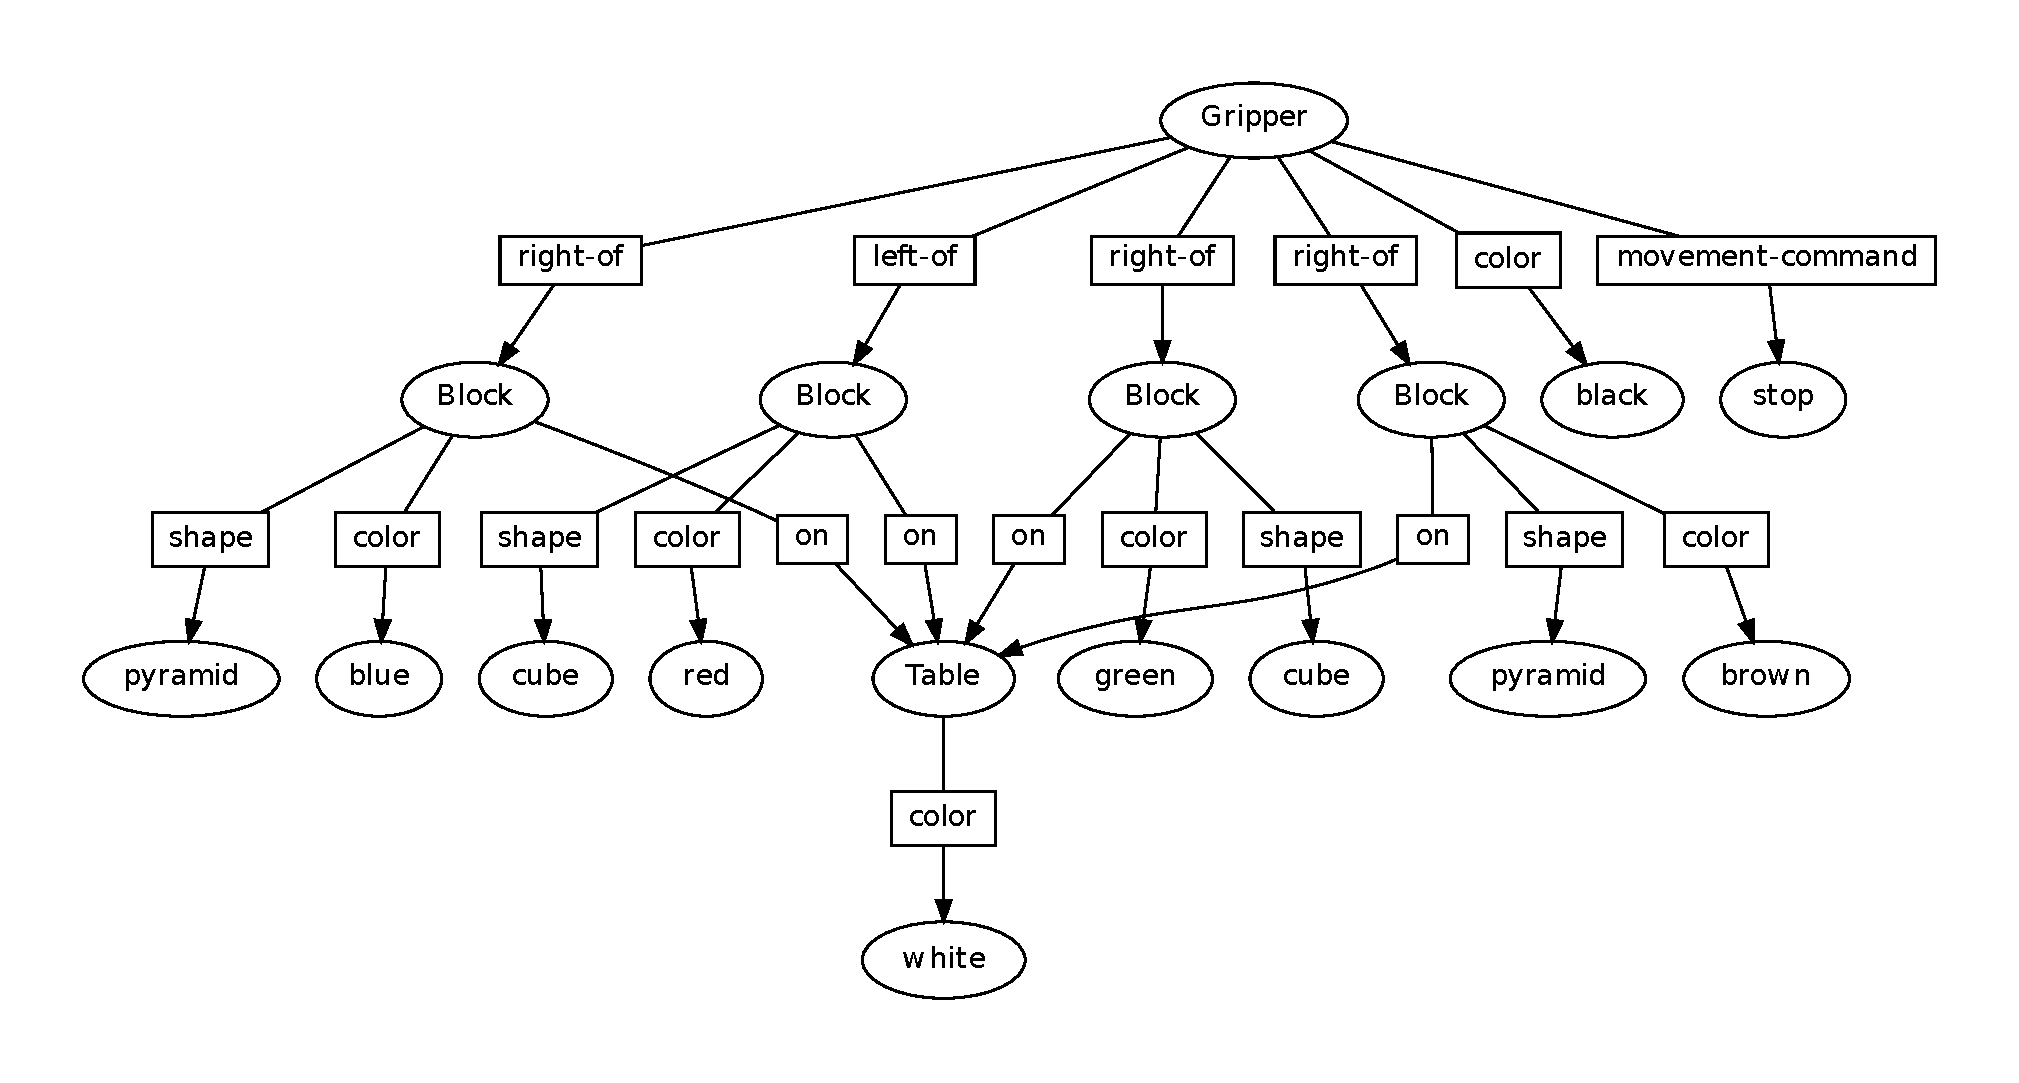
\includegraphics[width=14cm]{gfx/physical_knowledge_base_graph}
\caption[A graph representation of the physical knowledge base.]{A
  graph representation of the physical knowledge base, where
  frame-based objects become interconnected collections of elliptical
  node labels and rectangular edge labels.  This representation is
  consistent with the physical situation shown previously on
  {\mbox{page~\pageref{figure:introduction_example_problem_domain__duplicate_1}}}
  in
  {\mbox{\autoref{figure:introduction_example_problem_domain__duplicate_1}}}.}
\label{figure:physical_knowledge_base_graph}
\end{figure}

\section{The Deliberative Layer}
\label{section:the_deliberative_layer}

The deliberative layer is the first planning layer in the SALS
cognitive architecture.  The deliberative layer tries to accomplish
goals that are partial states of the physical knowledge base in the
learned reactive layer.
{\mbox{\autoref{figure:deliberative_and_learning_reactive_layers}}}
shows an overview of the deliberative layer and its connections to the
learned reactive layer below.  The following are functional
explanations of the labeled parts, A--G, in
{\mbox{\autoref{figure:deliberative_and_learning_reactive_layers}}}:
\begin{figure}
\hspace{-3cm}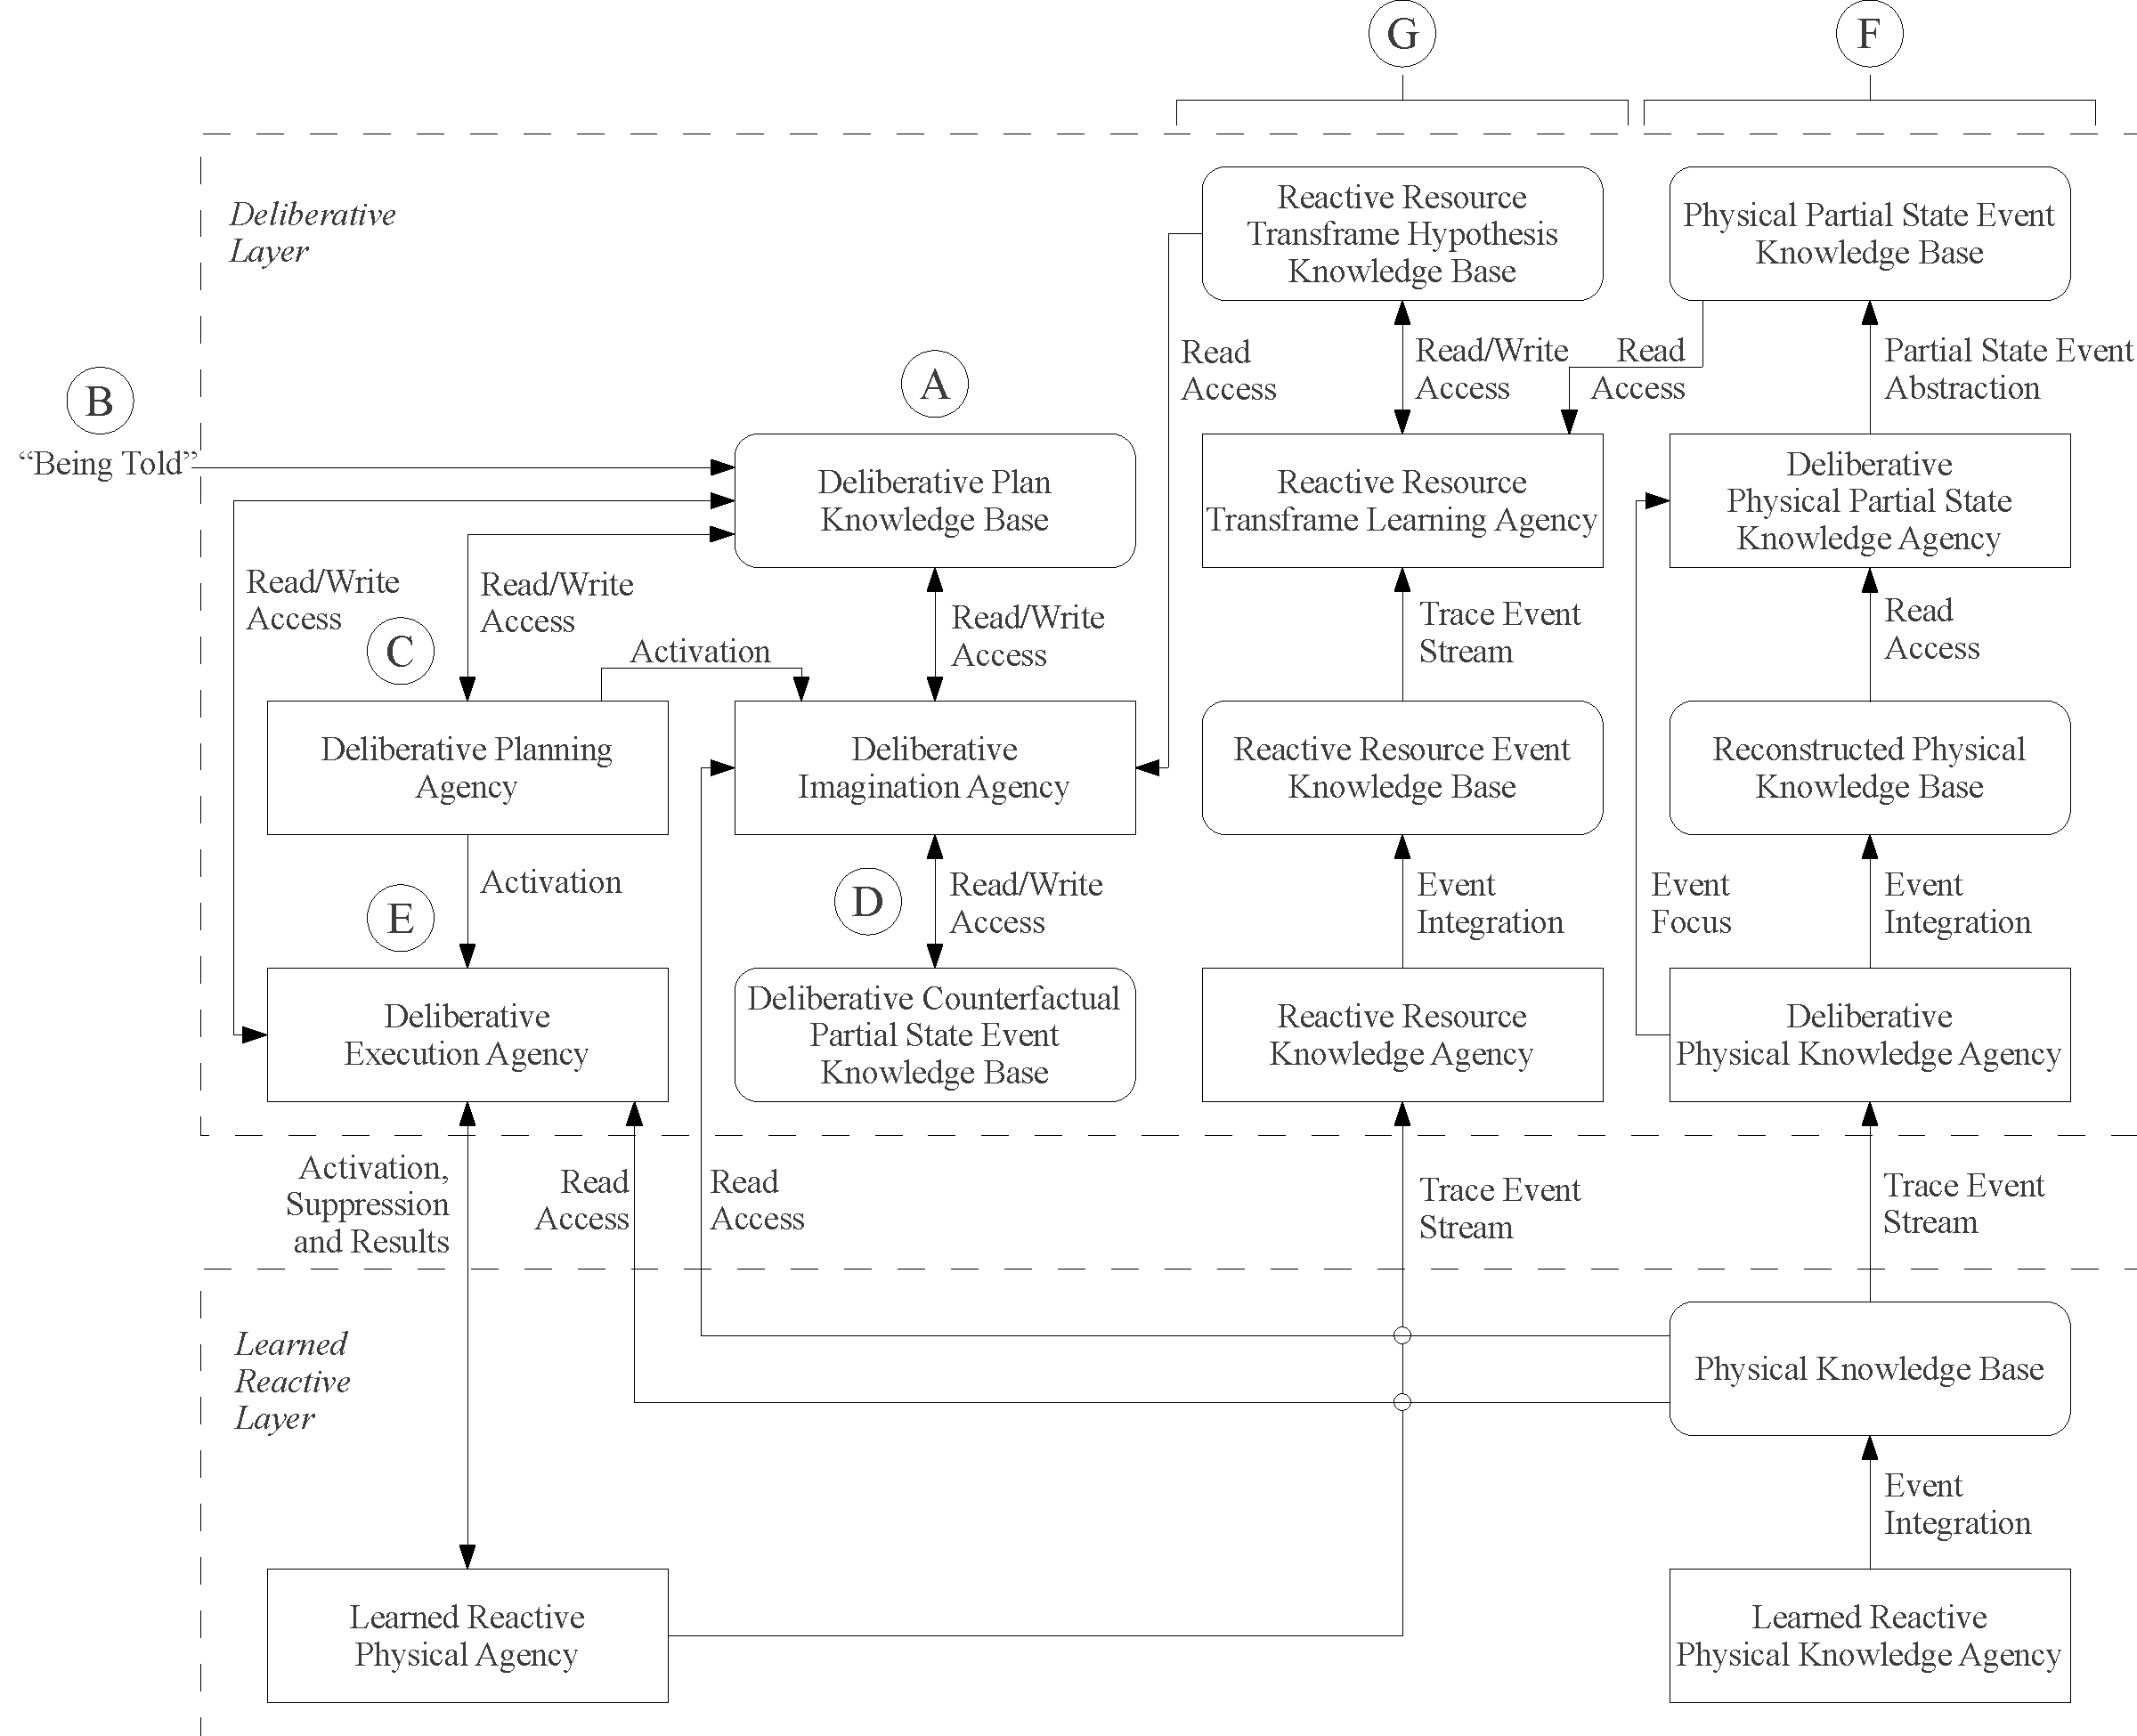
\includegraphics[width=16cm]{gfx/deliberative_and_learned_reactive_layers}
\caption[The deliberative layer and its connections to the learned
  reactive layer.]{The deliberative layer and its connections to the
  learned reactive layer.  See text in
  {\mbox{\autoref{section:the_deliberative_layer}}} for descriptions
  of labeled functional areas, A--G.}
\label{figure:deliberative_and_learning_reactive_layers}
\end{figure}
\begin{enumerate}[~~A.]
\item Natural language plans can enter the {\emph{deliberative plan
    knowledge base}} from outside of the AI by ``being told'' by a
  human user or another AI.  One such natural language plan that has
  been told to the SALS AI is to ``{\tt{stack a cube on a pyramid}}.''
\item The {\emph{deliberative plan knowledge base}} is where all
  deliberative natural language plans for physical action are stored
  along with the state of the deliberative planning machine and plan
  failures.  When natural language plans are told to the deliberative
  layer of the SALS AI, the plan is stored in the deliberative plan
  knowledge base.  When plans are manipulated and new plans are
  created, these new plans are also stored in the deliberative plan
  knowledge base.  In the example story presented in
  {\mbox{\autoref{chapter:introduction}}}, the deliberative planning
  machine focuses on a plan to ``{\tt{stack a cube on pyramid}}.''  At
  this point in the example story, the fact that the deliberative
  planning machine is focused on this plan is also stored as knowledge
  in the deliberative plan knowledge base: ``{\tt{a}}
  {\tt{deliberative}} {\tt{planning}} {\tt{machine}} {\tt{is}}
  {\tt{focused}} {\tt{on}} {\tt{a}} {\tt{plan}} {\tt{to}} {\tt{stack}}
  {\tt{a}} {\tt{cube}} {\tt{on}} {\tt{a}} {\tt{pyramid}}.''  Details
  of the internal representation of the deliberative plan knowledge
  base will be described in
  {\mbox{\autoref{section:the_deliberative_plan_knowledge_base}}}.
  The state of the deliberative plan knowledge base is reflected upon
  by the reflective layer, which will be described in
  {\mbox{\autoref{section:the_reflective_layer}}}.
\item The {\emph{deliberative planning agency}} contains the resources
  for planning activities that manipulate plans in the deliberative
  plan knowledge base as well as resources that in turn activate the
  resources in the neighboring deliberative imagination and execution
  agencies.  The deliberative planning agency includes resources that
  cause the imagination of the effects of a plan in focus, change the
  planning focus, manipulate plans currently in focus, as well as
  cause the execution of plans currently in focus.  The reflective
  layer, described in {\mbox{\autoref{section:the_reflective_layer}}},
  activates the resources in the deliberative planning agency to
  control the deliberative planning machine.
\item The {\emph{deliberative imagination agency}} imagines the
  hypothetical future effects of executing deliberative plans for
  physical action.  The {\emph{deliberative counterfactual partial
      state event knowledge base}} is used as a scratchpad for storing
  these hypothetical future physical states.  The current state of the
  physical knowledge base in the layer below is used as a starting
  point for the counterfactual knowledge created by the deliberative
  imagination agency.  For example, when the deliberative planning
  agency focuses the planning machine on the plan to ``{\tt{stack a
      cube on a pyramid}}'' and subsequently activates the
  deliberative imagination agency, the effects of the plan are
  imagined and the deliberative counterfactual partial state event
  knowledge base subsequently contains the physical partial state for
  ``{\tt{a cube to be on a pyramid}}.''
\item The {\emph{deliberative execution agency}} executes plans by
  activating and suppressing resources in the learned reactive
  physical agency in the layer below.  For example, when the
  deliberative planning agency focuses the planning machine on the
  plan to ``{\tt{stack a cube on a pyramid}}'' and subsequently
  activates the deliberative execution agency, the body of the plan is
  executed, including activating resources in the physical agency to
  ``{\tt{move right}},'' ``{\tt{grab}},'' ``{\tt{move left}},'' and
  ``{\tt{drop}}.''
\item A column of agencies and knowledge bases abstract partial states
  from the physical knowledge base in the learned reactive layer
  below.  Because partial state abstraction can be a slow process,
  this process is performed asynchronously based on a stream of change
  events.  A detailed description of partial states and their
  asynchronous abstraction will be given in
  {\mbox{\autoref{chapter:learning_asynchronously_from_experience}}},
  {\mbox{\autoref{section:partial_state_event_abstraction}}}.
  Abstracted partial state event knowledge is stored in the
  {\emph{physical partial state event knowledge base}}.  The
  abstraction of partial states is one of two types of asynchronous
  processing streams that constitute the SALS AI's ability to learn
  from the experience of executing plans.
\item A column of agencies and knowledge bases perform asynchronous
  learning of abstract causal rule hypotheses from physical agency
  resource execution preconditions.  The advantage of an asynchronous
  learning algorithm is that it does not slow down the execution of
  plans in the deliberative layer.  Historical versions of knowledge
  bases are reconstructed so that the slower learning algorithms can
  discover relevant patterns in this data for predicting the effects
  of actions.  For example, when the deliberative execution agency
  executes the plan ``{\tt{stack a cube on a pyramid}},'' the SALS AI
  learns that when ``{\tt{a gripper is holding a cube}}'' and ``{\tt{a
      pyramid is below a gripper}},'' the resulting state will
  {\emph{not}} be ``{\tt{a cube is on a pyramid}}.''  The details of
  the asynchronous learning of abstract causal rules from the
  experience of executing plans will be described in
  {\mbox{\autoref{chapter:learning_asynchronously_from_experience}}},
  {\mbox{\autoref{section:resource_execution_event_causal_rule_learning}}}.
\end{enumerate}

\subsection{The Deliberative Plan Knowledge Base}
\label{section:the_deliberative_plan_knowledge_base}

The {\emph{deliberative plan knowledge base}} is the heart of the
deliberative layer, where all deliberative natural language plans for
physical action are stored along with the deliberative planning
machine and deliberative plan failures.  Natural language plans can
enter the deliberative plan knowledge base from outside of the AI by
``being told,'' which is a form of natural language programming,
possibly in the form of an natural language expression from the user.
The {\emph{deliberative planning agency}} is the center of executive
control in the deliberative layer.  The deliberative planning agency
manipulates plans and also activates the {\emph{deliberative
    imagination agency}} and the {\emph{deliberative execution
    agency}} when these plans should be imagined or executed.  The
deliberative imagination agency uses learned rules that map
preconditions of learned reactive physical agency resource activations
to changes that these resources cause to occur in the learned reactive
physical knowledge base.  The deliberative imagination agency uses the
{\emph{deliberative counterfactual partial state event knowledge
    base}} as a scratchpad that can store hypothetical future states
of the learned reactive physical knowledge base if the appropriate
learned reactive physical agency resources are activated.  Once the
deliberative planning agency has decided to execute a given plan, the
deliberative execution agency is activated, which executes plans by
activating and suppressing resources in the learned reactive physical
agency in the layer below.

Similar to the visual and physical knowledge bases, the deliberative
plan knowledge base also consists of collections of interconnected
frame-based objects.  The following are different possible property
slots and symbolic values for the deliberative objects in the
deliberative plan knowledge base:
\begin{samepage}
  \begin{packed_itemize}
  \item{{\emph{type}}: $\{$``{\tt{plan}}'', ``{\tt{planner}}'', ``{\tt{execution-node}}'', ``{\tt{failure}}''$\}$}
  \item{{\emph{has-been-imagined}}: $\{$``{\tt{true}}'', ``{\tt{false}}''$\}$}
  \item{{\emph{default-slot-value}}: $\{$all natural language strings$\}$}
  \item{{\emph{hypothesized-to-cause}}: $\{$all physical partial states$\}$}
  \item{{\emph{positive-goal}}: $\{$all physical partial states$\}$}
  \item{{\emph{negative-goal}}: $\{$all physical partial states$\}$}
  \end{packed_itemize}
\end{samepage}
These properties are examples of those aspects of the deliberative
thinking layer that the AI can reflectively see about a single
deliberative object, including the type, the default slot values of a
natural language plan, and the goals of a planner.  In addition to
each deliberative object having properties, each deliberative object
may have different types of relations to other deliberative objects
that the AI can reflectively perceive.  Some are these relations are
as follows:
\begin{samepage}
  \begin{packed_itemize}
  \item{\emph{focus-plan}}
  \item{\emph{execution-plan}}
  \item{\emph{imagination-failure}}
  \item{\emph{execution-failure}}
  \item{\emph{start-execution-node}}
  \item{\emph{previous}}
  \item{\emph{next}}
  \item{\emph{subnode}}
  \item{\emph{supernode}}
  \end{packed_itemize}
\end{samepage}
I will describe the details of the objects in the deliberative plan
knowledge base in {\mbox{\autoref{chapter:learning_from_being_told}}},
where I will describe learning from being told and the natural
language planning process.  A simplified graph representation of the
deliberative plan knowledge base is shown in
{\mbox{\autoref{figure:deliberative_plan_knowledge_base_graph}}}.
\label{page:deliberative_plan_knowledge_base_graph-label_descriptions}
\begin{figure}
\hspace{0cm}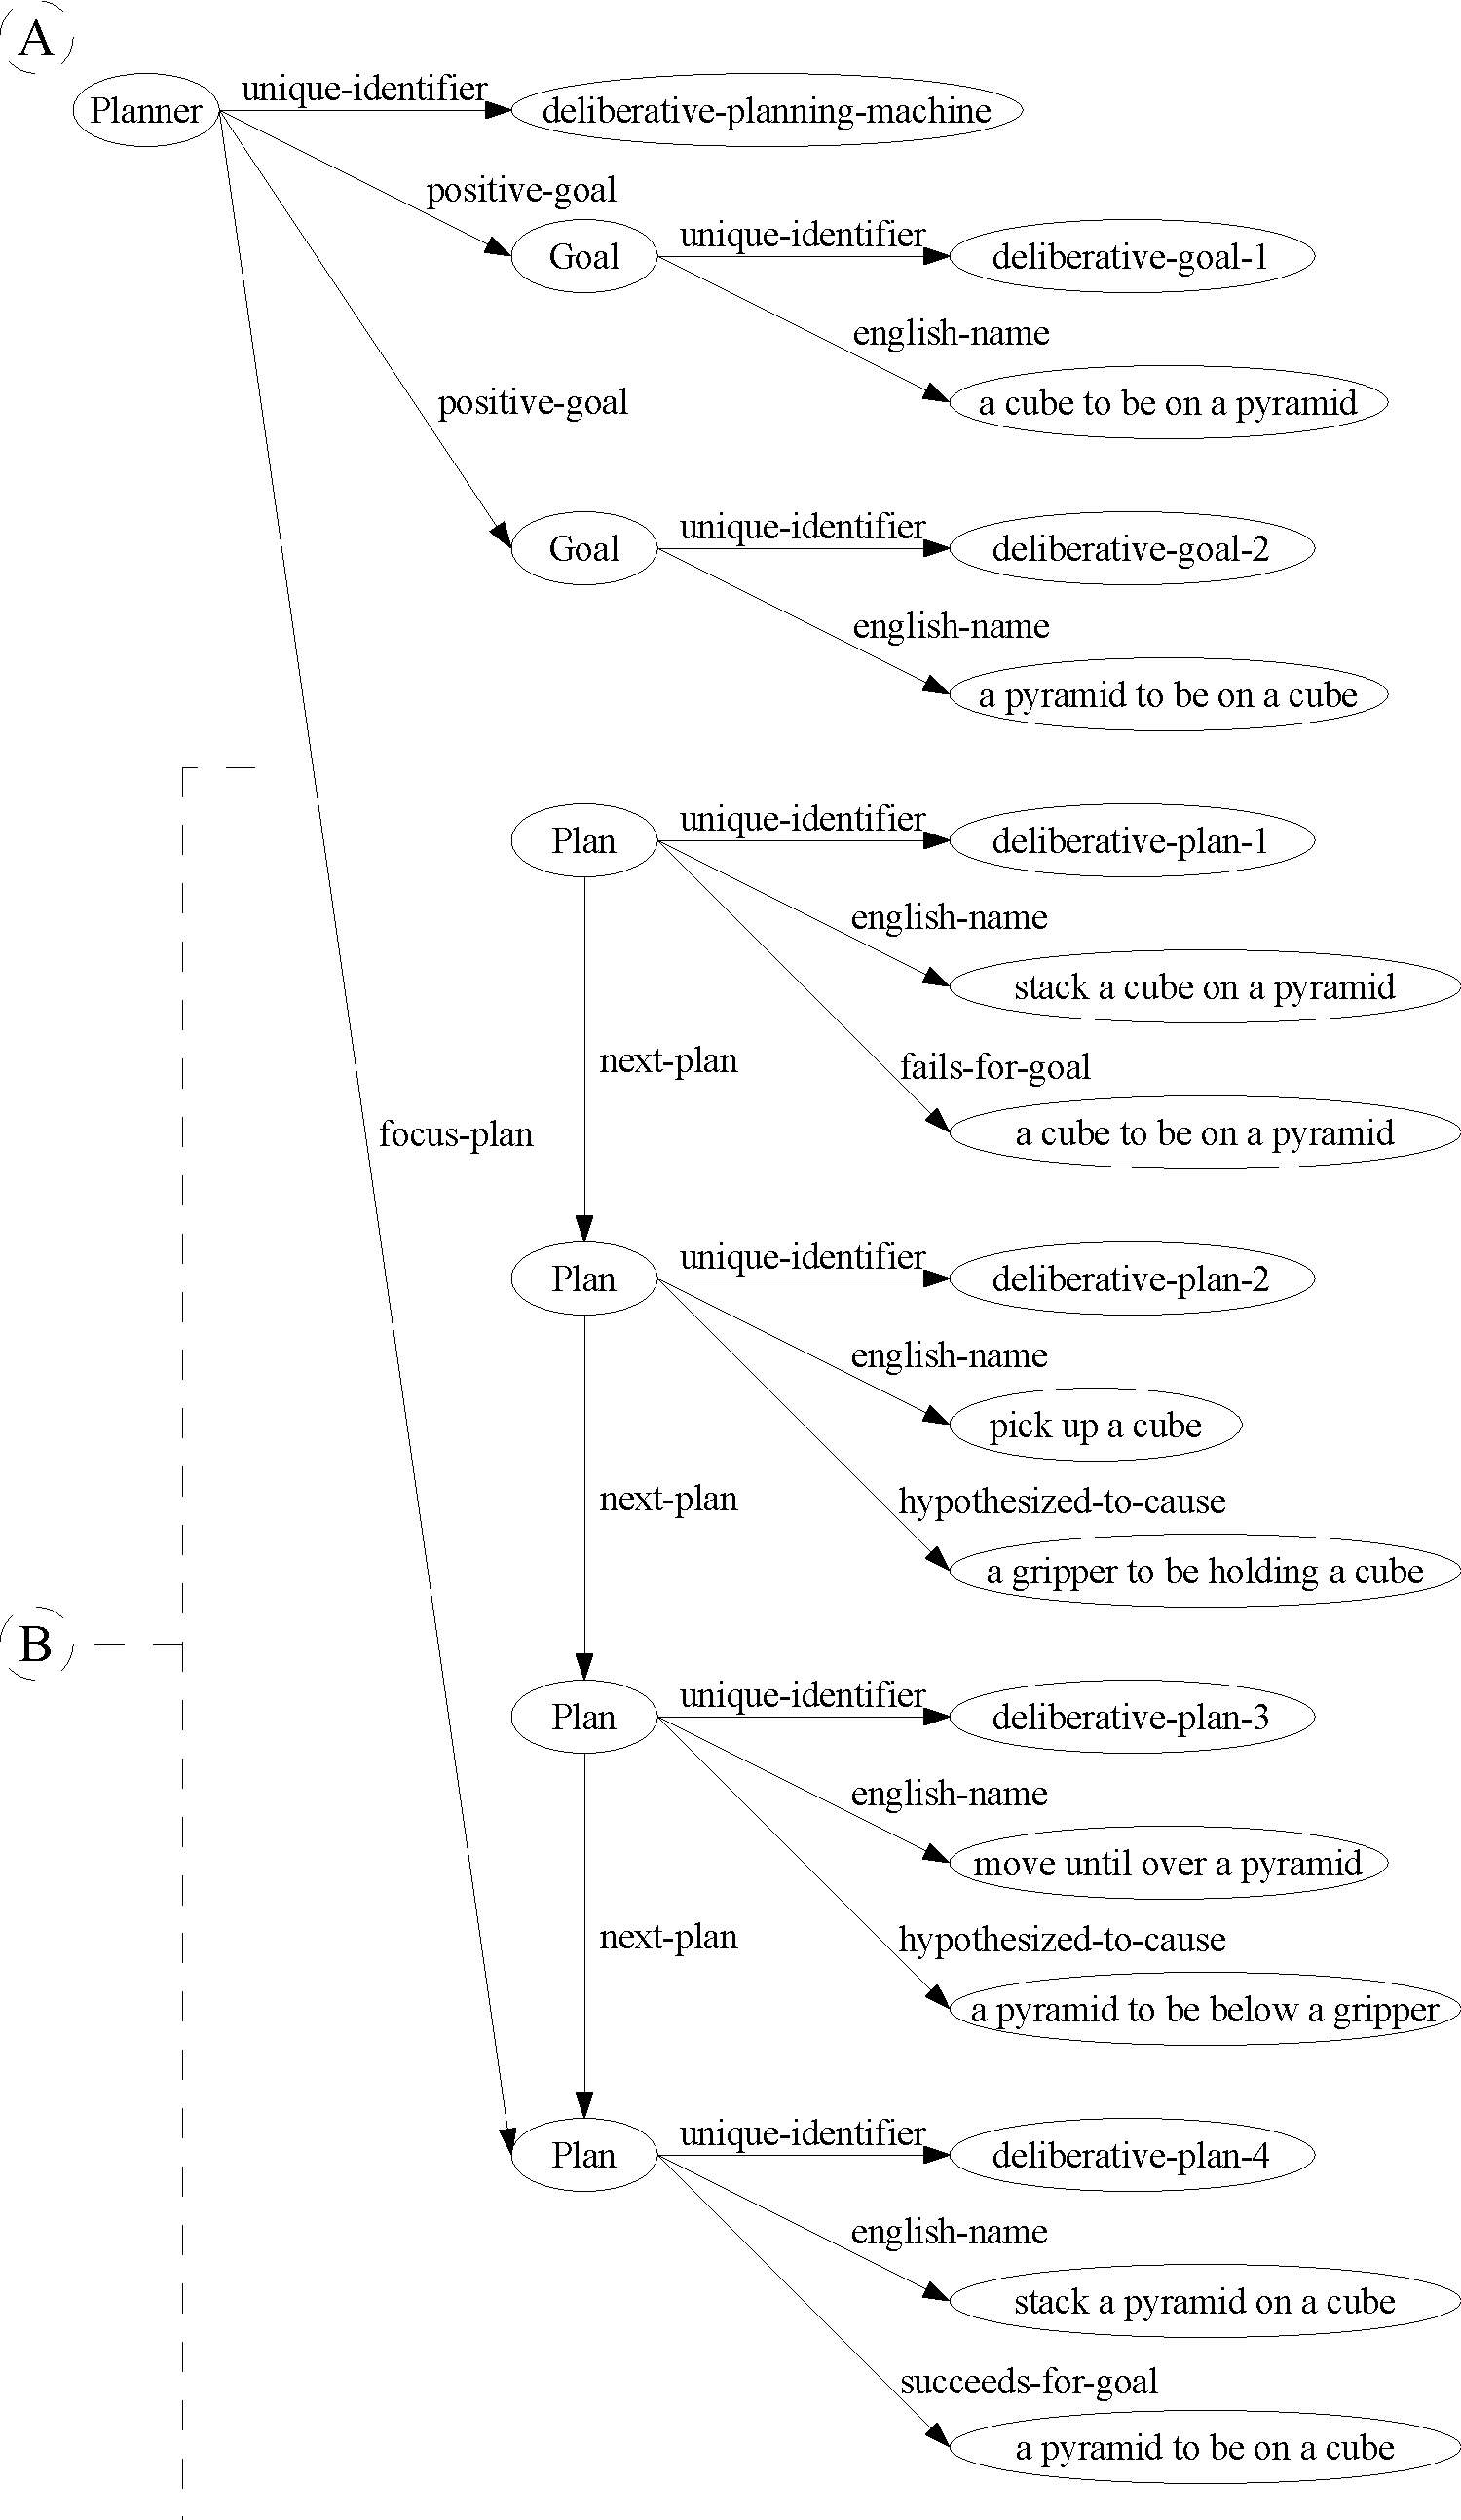
\includegraphics[height=20cm]{gfx/deliberative_plan_knowledge_base_graph-handdrawn}
\caption[Part of the deliberative plan knowledge base represented as a
  graph.]{Part of the deliberative plan knowledge base represented as
  a graph.  See text in
  {\mbox{\autoref{section:the_deliberative_plan_knowledge_base}}} on
  {\mbox{page~\pageref{page:deliberative_plan_knowledge_base_graph-label_descriptions}}}
  for descriptions of knowledge labels, {\mbox{A~and~B}}.}
\label{figure:deliberative_plan_knowledge_base_graph}
\end{figure}
In this figure, knowledge labels {\mbox{A~and~B}} refer to the
following different types of deliberative knowledge:
\begin{enumerate}[~~A.]
\item The state of the {\emph{deliberative planning machine}} includes
  positive and negative physical goals as well as references to plans
  for physical action that the planning machine is currently focusing
  on or executing.  For example, in the story presented in
  {\mbox{\autoref{chapter:introduction}}}, the plan to ``{\tt{want a
      block to be on a block}}'' is a reflective plan that has
  previously been told to the reflective layer of the SALS AI.  The
  execution of this reflective plan causes the deliberative planning
  machine to be given two specific positive goals for either ``{\tt{a
      cube to be on a pyramid}}'' or ``{\tt{a pyramid to be on a
      cube}}.''  At the end of the story, the reflective SALS AI
  successfully accomplishes its goal for ``{\tt{a pyramid to be on a
      cube}}'' by first focusing on the last plan that it has been
  told and then executing this plan.
\item Representations of deliberative plans are organized into a
  linked-list structure that goes forward and backward in time.  Plans
  that have been told to the SALS AI furthest in the past are at the
  beginning of the list.  In the example story, the SALS AI uses this
  linked-list structure to organize its search through deliberative
  plans for physical action.  Initially, the SALS AI considers plans
  from newest to oldest, which results in finding the plan,
  ``{\tt{stack a cube on a pyramid}},'' which fails to accomplish its
  goal for ``{\tt{a cube to be on a pyramid}}.''  Finally, the SALS AI
  searches through deliberative plans from oldest to newest and this
  results in finding the plan, ``{\tt{stack a pyramid on a cube}},''
  which succeeds in accomplishing its goal for ``{\tt{a pyramid to be
      on a cube}}.''  At this point in the example, the SALS AI
  reflectively learns to apply a different planning method for the
  current goals of the deliberative planning machine.
\end{enumerate}
%% \begin{sidewaysfigure}
%% \begin{center}
%% \includegraphics[width=8.5in]{gfx/deliberative_plan_knowledge_base_graph}
%% \end{center}
%% \hspace{4cm}\parbox{15cm}{\caption[A simplified graph representation
%%     of the deliberative plan knowledge base.]{A simplified graph
%%     representation of the deliberative plan knowledge base, where
%%     frame-based objects become interconnected collections of
%%     elliptical node labels and rectangular edge labels.  The
%%     deliberative planner node is at the top of the graph.  This
%%     planner is ``focused'' on a linked list of deliberative plan
%%     objects.  The planner has two goals: (1) ``{\tt{a pyramid to be on
%%         a cube}},'' and (2) ``{\tt{a cube to be on a pyramid}}.''  The
%%     causal effects of the first plan have been imagined and are listed
%%     as properties of the plan object.  The execution node structure of
%%     the deliberative imagination process are not shown for visual
%%     simplicity.}\label{figure:deliberative_plan_knowledge_base_graph}}
%% \end{sidewaysfigure}

\subsection{Asynchronous Learning}

To imagine the effects of executing plans, the deliberative layer
learns abstract hypothetical models of the effects of learned reactive
physical agency resource activations.  These learned models are
generated by a rule learning algorithm that predicts a hypothetical
{\emph{transframe}} \cite[]{minsky:1975} given the preconditions for
an action.  Transframes represent changes between one collection of
frames and another collection of frames.  The details of transframes
in the SALS AI will be discussed in
{\mbox{\autoref{chapter:learning_asynchronously_from_experience}}},
{\mbox{\autoref{section:resource_execution_event_causal_rule_learning}}}.
Asynchronous learning is implemented as two stages of stream
processing.  The first stage abstracts partial state events from a
trace event stream composed of any change events that occur in the
learned reactive physical knowledge base.  The second stage receives a
stream of activation and completion events from the learned reactive
physical agency resources.  Because both of these asynchronous stages
process different types of event streams at different rates, the
resulting knowledge bases are accurate for different points of time in
the past.  Although the timing of the two-staged asynchronous learning
in SALS complicates the implementation, the advantage is simple: the
execution of learned reactive physical agency resources and the
manipulation of the learned reactive physical knowledge base can both
operate at full speed, while the slower learning algorithm can operate
at its own pace.  In practice, resource activations and knowledge
changes occur in high-speed bursts, followed by periods of
deliberation, which generally gives the slower learning algorithms
time to catch up.  The details of the SALS asynchronous learning
algorithm will be discussed in
{\mbox{\autoref{chapter:learning_asynchronously_from_experience}}}.

\section{The Reflective Layer}
\label{section:the_reflective_layer}

While the deliberative layer focuses on learning the effects of
physical actions to make plans to control the physical knowledge base,
the reflective layer focuses on learning the effects of deliberative
planning actions to make plans to control the deliberative plan
knowledge base.  This similarity is abstracted in SALS and is called a
{\emph{planning layer}}.  The deliberative, reflective, and
super-reflective layers are all instantiations of these planning layer
cognitive architectural objects.  A planning layer is an extension
that can be added to any paired combination of a knowledge base and an
agency of resources to learn how to use to control the partial states
within the knowledge base.
{\mbox{\autoref{figure:reflective_and_deliberative_layers}}} shows the
reflective layer and its connection to the deliberative layer.  While
the deliberative layer focuses on learning about making plans to
control the physical knowledge base, the reflective layer focuses on
learning about making plans to control the deliberative plan knowledge
base.  This similarity is abstracted in SALS and is called a
{\emph{planning layer}}.  The deliberative, reflective, and
super-reflective layers are all instantiations of these planning layer
cognitive architectural objects.
\begin{figure}
\hspace{-3cm}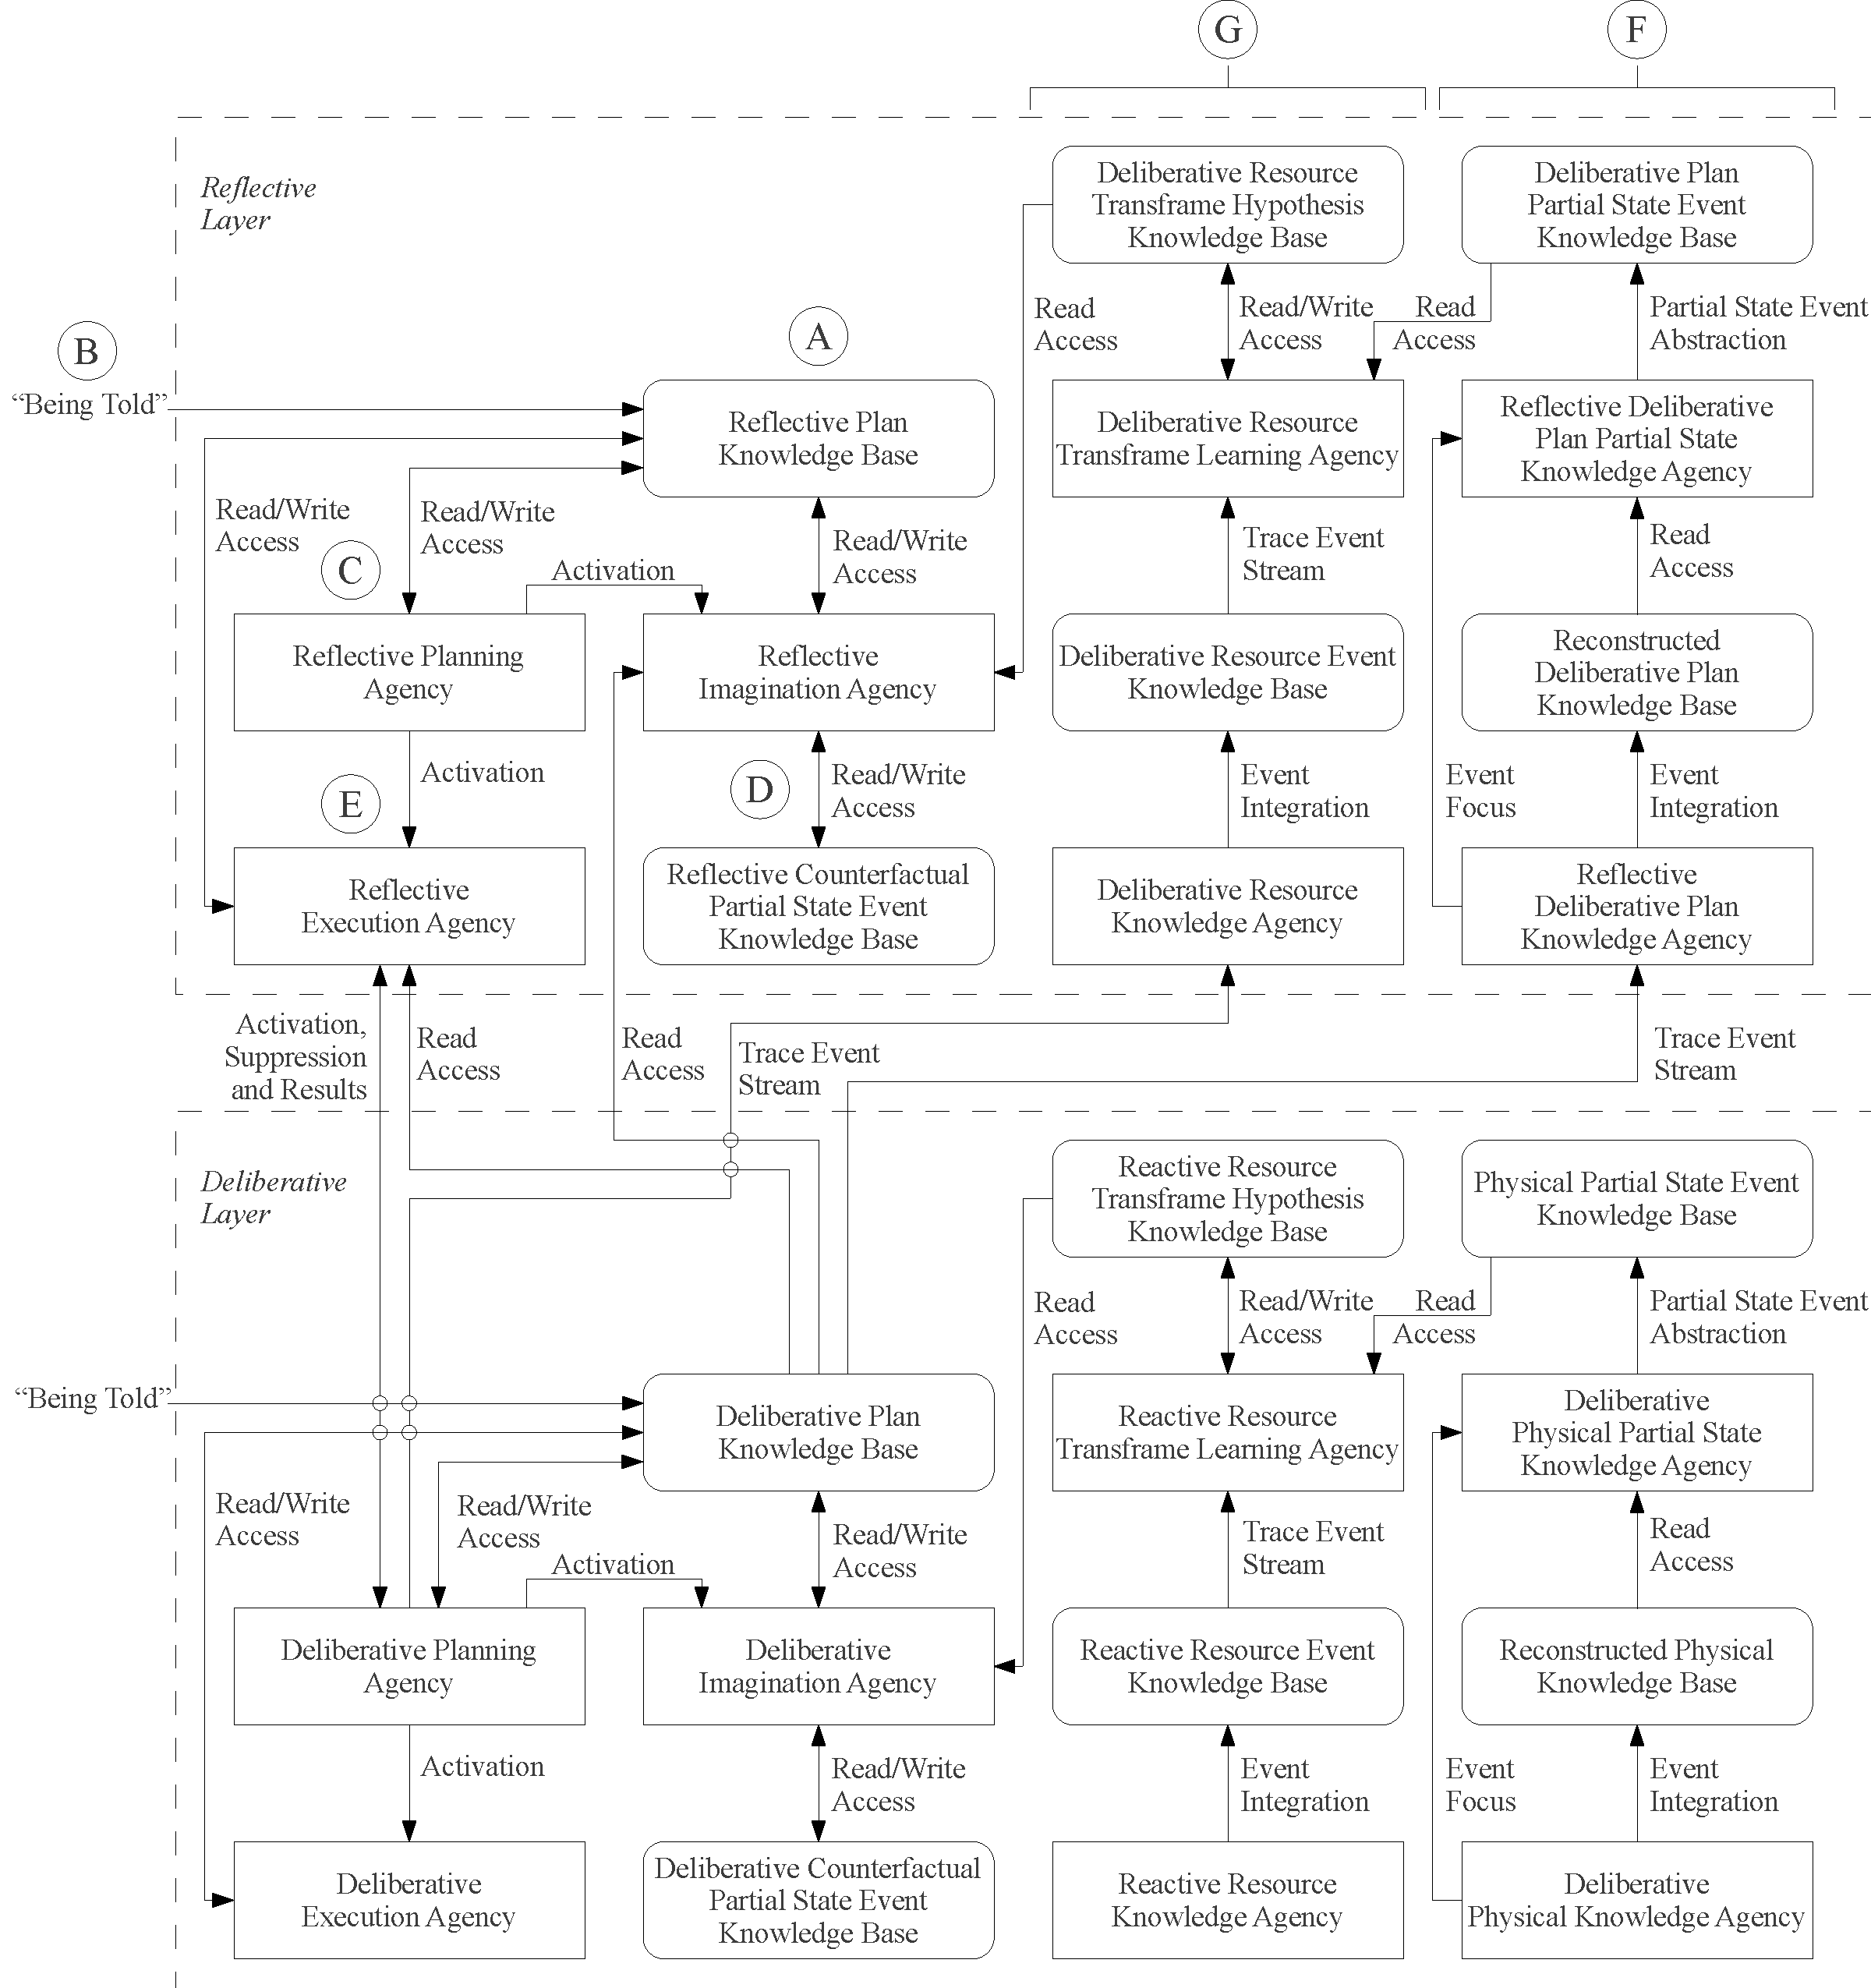
\includegraphics[width=16cm]{gfx/reflective_and_deliberative_layers}
\caption[The reflective layer and its connection to the deliberative
  layer.]{The reflective layer and its connection to the deliberative
  layer is analogous to the deliberative layer and its connection to
  the learned reactive layer, shown in
  {\mbox{\autoref{figure:physical_knowledge_base_graph}}} on
  {\mbox{page~\pageref{figure:physical_knowledge_base_graph}}}.  See
  text in {\mbox{\autoref{section:the_reflective_layer}}} for
  descriptions of labeled functional areas, A--G.}
\label{figure:reflective_and_deliberative_layers}
\end{figure}
\begin{enumerate}[~~A.]
\item Natural language plans can enter the {\emph{reflective plan
    knowledge base}} from outside of the AI by ``being told'' by a
  human user or another AI.  One such reflective natural language plan
  that has been told to the SALS AI in the example presented in
  {\mbox{\autoref{chapter:introduction}}} is to ``{\tt{find an old
      plan to accomplish a goal}}.''  Plans in the reflective plan
  knowledge base include different methods for how to find or create
  plans to accomplish different types of physical partial states, or
  deliberative goals.
\item The {\emph{reflective plan knowledge base}} is where all
  reflective natural language plans for deliberative action are stored
  along with the state of the reflective planning machine and
  reflective plan failures.  When natural language plans are told to
  the reflective layer of the SALS AI, the plan is stored in the
  reflective plan knowledge base.  In the example story presented in
  {\mbox{\autoref{chapter:introduction}}}, the reflective planning
  machine focuses on a plan to ``{\tt{find a recent plan to accomplish
      a goal}}.''  At this point in the example story, the fact that
  the reflective planning machine is focused on this plan is also
  stored as knowledge in the reflective plan knowledge base:
  ``{\tt{a}} {\tt{reflective}} {\tt{planning}} {\tt{machine}}
  {\tt{is}} {\tt{focused}} {\tt{on}} {\tt{a}} {\tt{plan}} {\tt{to}}
  {\tt{find}} {\tt{a}} {\tt{recent}} {\tt{plan}} {\tt{to}}
  {\tt{accomplish}} {\tt{a}} {\tt{goal}}.''  Details of the internal
  representation of the reflective plan knowledge base will be
  described in
  {\mbox{\autoref{section:the_reflective_plan_knowledge_base}}}.  The
  state of the reflective plan knowledge base is further reflected
  upon by the super-reflective layer, which will be described in
  {\mbox{\autoref{section:the_super_reflective_layer}}}.
\item The {\emph{reflective planning agency}} contains the resources
  for reflective planning activities that manipulate plans in the
  reflective plan knowledge base as well as resources that in turn
  activate the resources in the neighboring reflective imagination and
  execution agencies.  The reflective planning agency includes
  resources that cause the imagination of the effects of a reflective
  plan in focus, change the reflective planning focus, manipulate
  reflective plans currently in focus, as well as cause the execution
  of reflective plans currently in focus.  The super-reflective layer,
  described in {\mbox{\autoref{section:the_super_reflective_layer}}},
  activates the resources in the reflective planning agency to control
  the reflective planning machine.
\item The {\emph{reflective imagination agency}} imagines the
  hypothetical future effects of executing reflective plans for
  deliberative action.  The {\emph{reflective counterfactual partial
      state event knowledge base}} is used as a scratchpad for storing
  these hypothetical future deliberative states.  The current state of
  the deliberative plan knowledge base in the layer below is used as a
  starting point for the counterfactual knowledge created by the
  reflective imagination agency.  For example, when the reflective
  planning agency focuses the reflective planning machine on the plan
  to ``{\tt{find a recent deliberative plan to accomplish a goal}}''
  and subsequently activates the reflective imagination agency, the
  effects of the plan are imagined and the reflective counterfactual
  partial state event knowledge base subsequently contains the
  deliberative partial state for ``{\tt{a plan has an expectation
      failure}}.''  This prediction of plan failure does not require
  the deliberative layer to imagine the physical effects of executing
  physical actions; instead, plan failure is predicted reflectively
  from the structure of the deliberative plan and its relationship to
  the deliberative planning machine, including the current
  deliberative goals.
\item The {\emph{reflective execution agency}} executes reflective
  plans by activating and suppressing resources in the deliberative
  plan agency in the layer below.  For example, when the reflective
  planning agency focuses the reflective planning machine on the plan
  to ``{\tt{find a recent deliberative plan to accomplish a goal}}''
  and subsequently activates the reflective execution agency, the body
  of the plan is executed, including activating resources in the
  deliberative plan agency to ``{\tt{focus}} {\tt{on}} {\tt{most}}
  {\tt{recent}} {\tt{plan}},'' ``{\tt{focus}} {\tt{on}}
  {\tt{previous}} {\tt{plan}},'' ``{\tt{imagine}} {\tt{effects}}
  {\tt{of}} {\tt{plan}} {\tt{in}} {\tt{focus}},'' and ``{\tt{execute}}
  {\tt{plan}} {\tt{in}} {\tt{focus}}.''
\item A column of agencies and knowledge bases abstract partial states
  from the deliberative plan knowledge base in the deliberative layer
  below.  Because partial state abstraction can be a slow process,
  this process is performed asynchronously based on a stream of change
  events.  A detailed description of partial states and their
  asynchronous abstraction will be given in
  {\mbox{\autoref{chapter:learning_asynchronously_from_experience}}},
  {\mbox{\autoref{section:partial_state_event_abstraction}}}.
  Abstracted partial state event knowledge is stored in the
  {\emph{deliberative plan partial state event knowledge base}}.  The
  abstraction of partial states is one of two types of asynchronous
  processing streams that constitute the SALS AI's ability to learn
  from the experience of executing plans.
\item A column of agencies and knowledge bases perform asynchronous
  learning of abstract causal rule hypotheses from deliberative plan
  agency resource execution preconditions.  The advantage of an
  asynchronous learning algorithm is that it does not slow down the
  execution of plans in the reflective layer.  Historical versions of
  the deliberative plan knowledge base are reconstructed so that the
  slower learning algorithms in the reflective layer can discover
  relevant patterns in this data for predicting the effects of
  deliberative actions.  For example, when the reflective execution
  agency executes the plan to ``{\tt{find a recent deliberative plan
      to accomplish a goal}},'' the SALS AI learns that when ``{\tt{a
      planner has the goal for a cube to be on a pyramid}}'' and
  ``{\tt{a planner has the goal for a pyramid to be on a cube}},'' the
  resulting state will be ``{\tt{a plan has an expectation
      failure}}.''  The details of the asynchronous learning of
  abstract causal rules from the experience of executing plans will be
  described in
  {\mbox{\autoref{chapter:learning_asynchronously_from_experience}}},
  {\mbox{\autoref{section:resource_execution_event_causal_rule_learning}}}.
\end{enumerate}

\subsection{The Reflective Plan Knowledge Base}
\label{section:the_reflective_plan_knowledge_base}

A simplified graph representation of the reflective plan knowledge
base is shown in
{\mbox{\autoref{figure:reflective_plan_knowledge_base_graph}}}.
\label{page:reflective_plan_knowledge_base_graph-label_descriptions}
\begin{figure}
\hspace*{-2cm}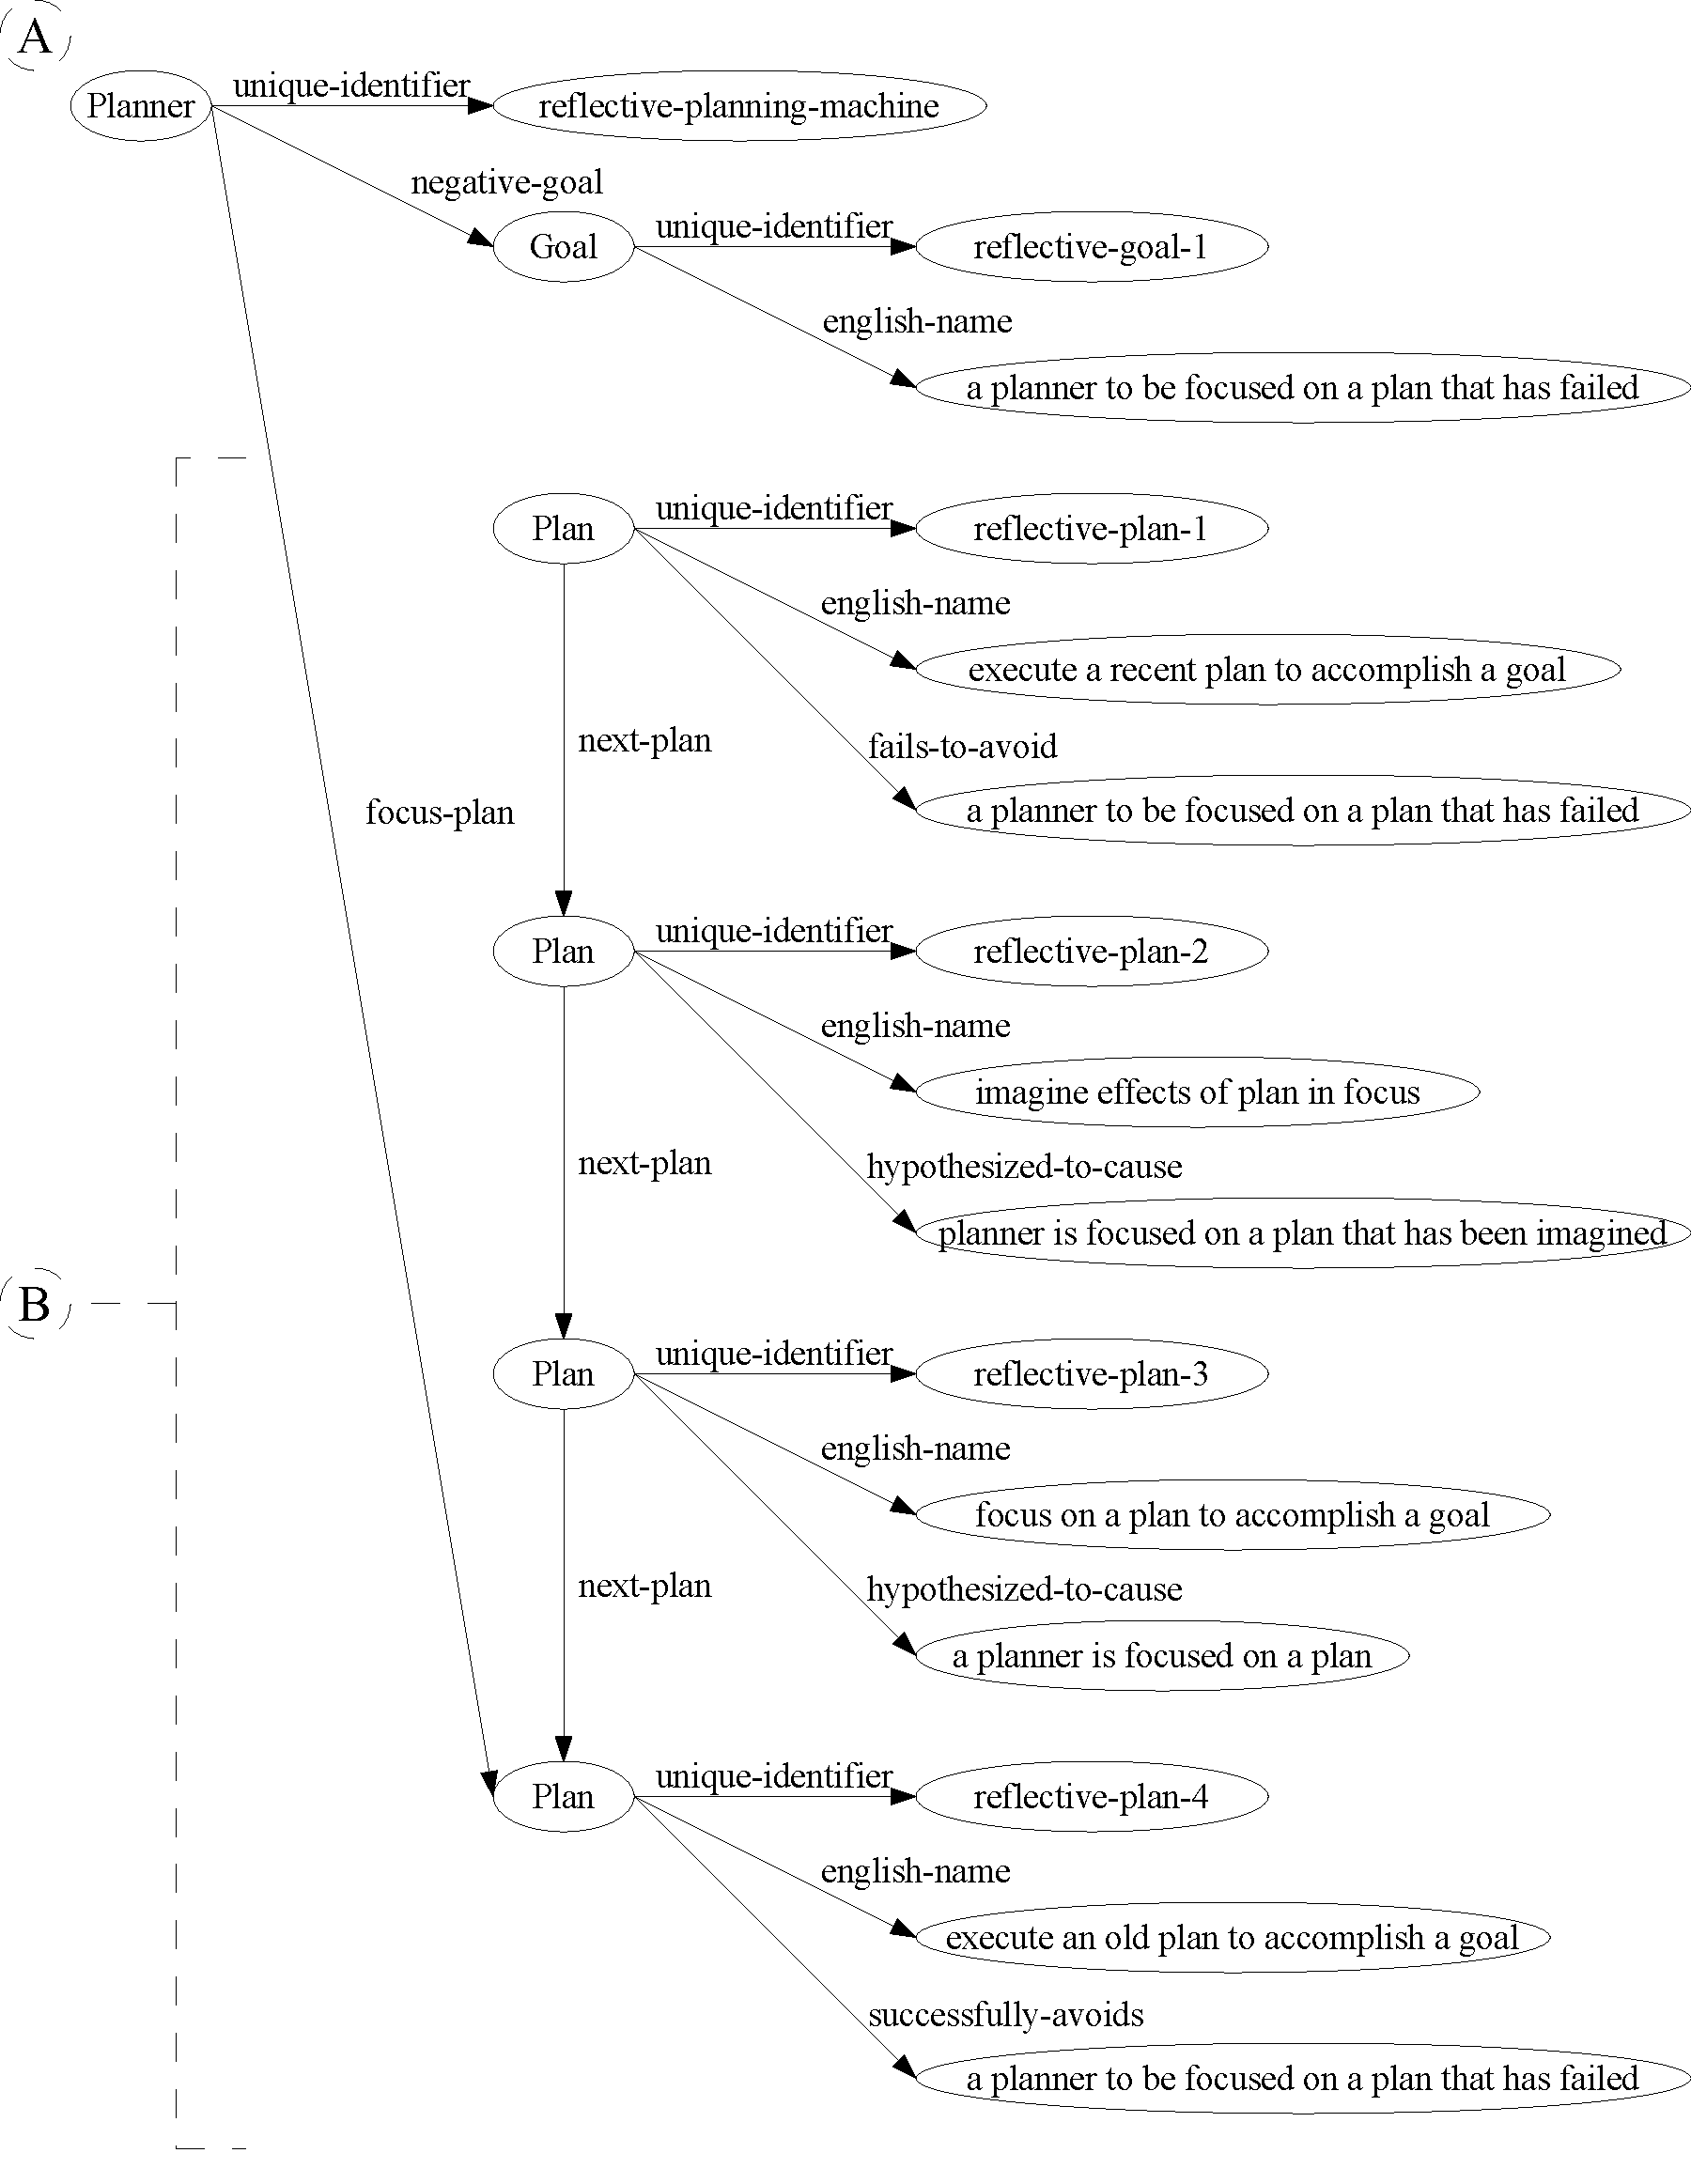
\includegraphics[height=20cm]{gfx/reflective_plan_knowledge_base_graph-handdrawn}
\caption[Part of the reflective plan knowledge base represented as a
  graph.]{Part of the reflective plan knowledge base represented as a
  graph.  See text in
  {\mbox{\autoref{section:the_reflective_plan_knowledge_base}}} on
  {\mbox{page~\pageref{page:reflective_plan_knowledge_base_graph-label_descriptions}}}
  for descriptions of knowledge labels, {\mbox{A~and~B}}.}
\label{figure:reflective_plan_knowledge_base_graph}
\end{figure}
In this figure, knowledge labels {\mbox{A~and~B}} refer to the
following different types of reflective knowledge:
\begin{enumerate}[~~A.]
\item The state of the {\emph{reflective planning machine}} includes
  positive and negative reflective goals as well as references to
  reflective plans for deliberative action.  For example, in the story
  presented in {\mbox{\autoref{chapter:introduction}}}, the reflective
  planning machine has the negative goal for avoiding ``{\tt{a}}
  {\tt{planner}} {\tt{to}} {\tt{be}} {\tt{focused}} {\tt{on}} {\tt{a}}
  {\tt{plan}} {\tt{that}} {\tt{has}} {\tt{failed}}.''  The reflective
  planning machine fails to avoid this deliberative partial state when
  it executes a plan to ``{\tt{execute}} {\tt{a}} {\tt{recent}}
  {\tt{plan}} {\tt{to}} {\tt{accomplish}} {\tt{a}} {\tt{goal}},''
  which leads to a failure while executing the deliberative plan to
  ``{\tt{stack}} {\tt{a}} {\tt{cube}} {\tt{on}} {\tt{a}}
  {\tt{pyramid}}.''
\item Representations of reflective plans are organized into a
  linked-list structure that goes forward and backward in time.  Plans
  that have been told to the SALS AI furthest in the past are at the
  beginning of the list.  In the example story, the SALS AI uses this
  linked-list structure to organize its search through reflective
  plans for deliberative action.  Initially, the SALS AI executes the
  reflective plan to ``{\tt{execute}} {\tt{a}} {\tt{recent}}
  {\tt{plan}} {\tt{to}} {\tt{accomplish}} {\tt{a}} {\tt{goal}},''
  which results in a search through deliberative plans for physical
  action starting with most recently learned deliberative plans.  This
  search method leads to a failure to accomplish a deliberative goal,
  one of the physical partial states for ``{\tt{a block to be on a
      block}}.''  The failure of the deliberative plan to ``{\tt{stack
      a cube on a pyramid}}'' subsequently causes the failure of the
  reflective plan to avoid the reflective goal of avoiding ``{\tt{a}}
  {\tt{deliberative}} {\tt{planner}} {\tt{to}} {\tt{be}}
  {\tt{focused}} {\tt{on}} {\tt{a}} {\tt{plan}} {\tt{that}} {\tt{has}}
  {\tt{failed}}.''  At this point in the example, the SALS AI
  reflectively learns to apply a different reflective plan given the
  state of the deliberative plan knowledge base, including the current
  deliberative goals.  The reflective plan to ``{\tt{execute}}
  {\tt{an}} {\tt{old}} {\tt{plan}} {\tt{to}} {\tt{accomplish}}
  {\tt{a}} {\tt{goal}}'' initiates a search through deliberative plans
  from oldest to newest, which results in accomplishing a positive
  deliberative goal and avoiding the negative reflective goal.  In
  this way, the SALS AI learns to apply different search strategies,
  or planning methods, for successfully accomplishing different types
  of goals, given feedback from the experience of actually executing
  the plans that it has found.
\end{enumerate}
%% \begin{sidewaysfigure}
%% \centering
%% \vspace{2cm}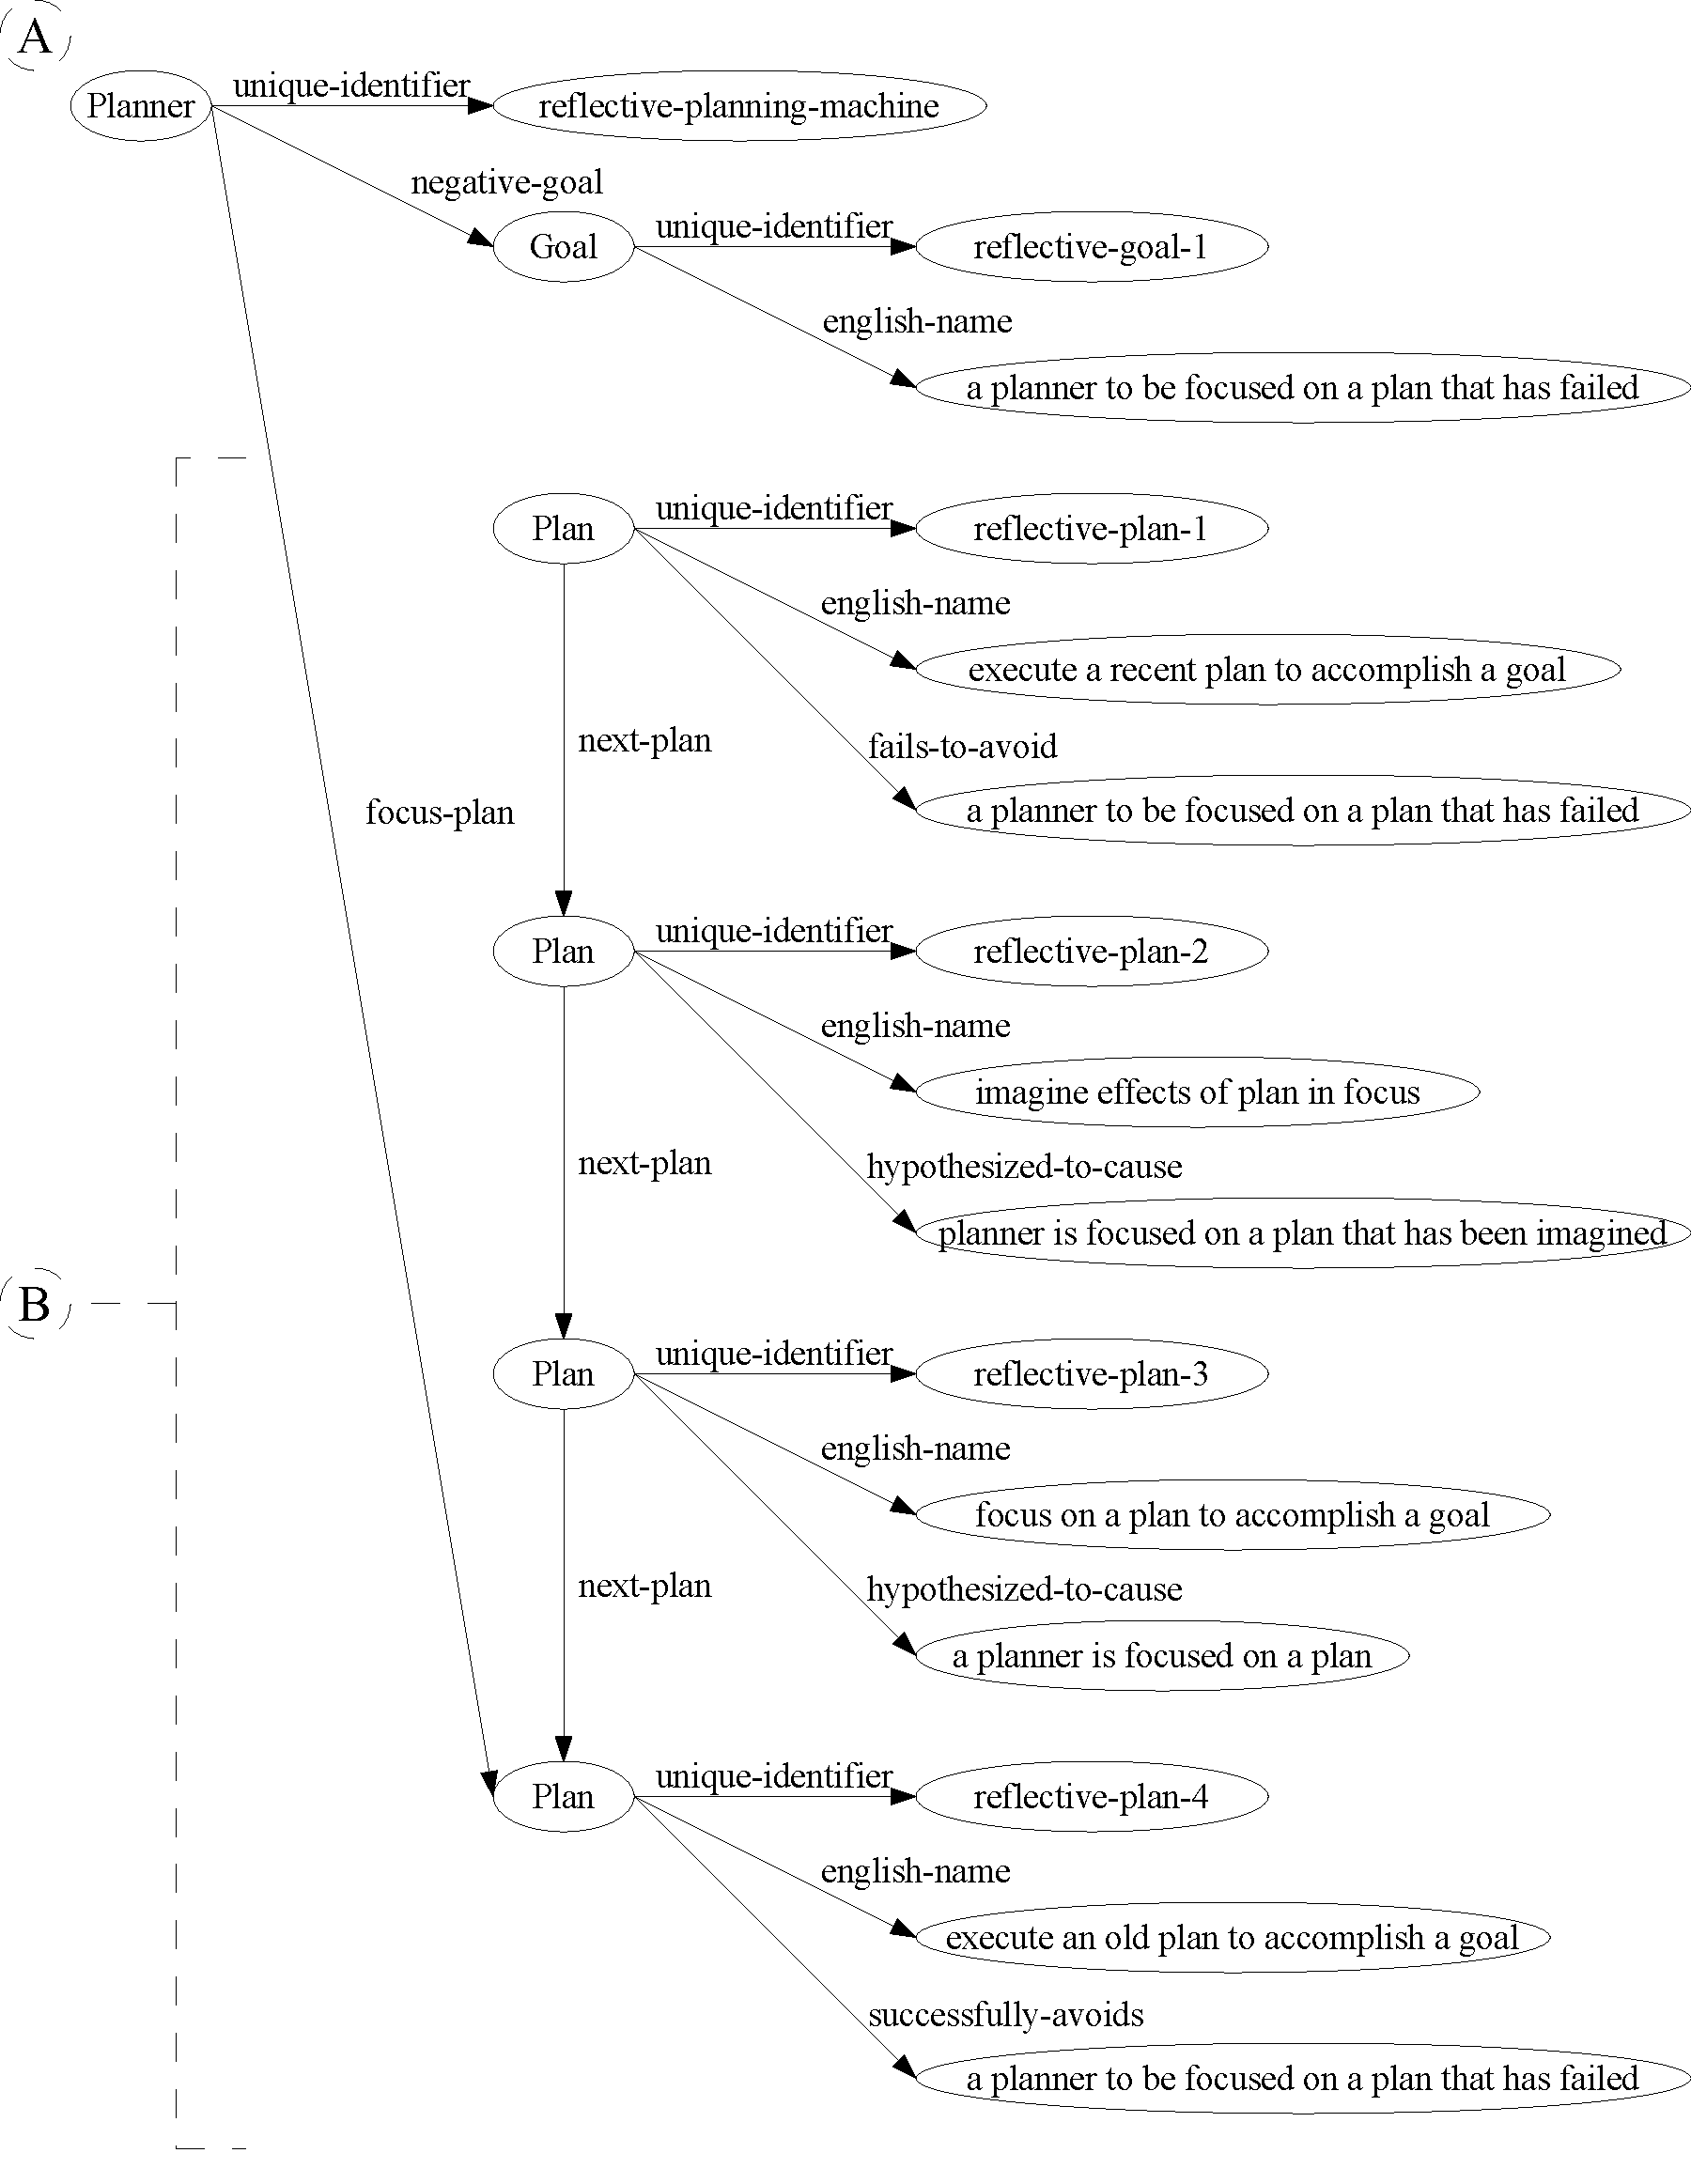
\includegraphics[height=5in]{gfx/reflective_plan_knowledge_base_graph-handdrawn}
%% \hspace{0cm}\parbox{15cm}{\caption[A simplified graph representation
%%     of the reflective plan knowledge base.]{A simplified graph
%%     representation of the reflective plan knowledge base, where
%%     frame-based objects become interconnected collections of
%%     elliptical node labels and rectangular edge labels.  The
%%     reflective planner node is at the top of the graph.  This planner
%%     is ``focused'' on a linked list of reflective plan objects.  The
%%     planner has one negative goal: ``{\tt{a planner to be focusing on
%%         a plan that has failed}}.''  The causal effects of the first
%%     plan have been imagined and are listed as properties of the plan
%%     object.  The execution node structure of the reflective
%%     imagination process are not shown for visual simplicity.  Note
%%     that the partial states in the reflective plan knowledge base are
%%     about the deliberative plan knowledge
%%     base.}\label{figure:reflective_plan_knowledge_base_graph}}
%% \end{sidewaysfigure}
Although the reflective layer of the SALS cognitive architecture is
superficially similar to the deliberative layer, the type of knowledge
that the reflective layer reasons about is categorically different.
While the deliberative layer plans toward relatively simple physical
goals, such as ``{\tt{a cube to be on a pyramid}},'' the partial
states in the reflective layer are the much more complex partial
states of the deliberative layer below, such as ``{\tt{a planner to be
    focusing on a plan that is hypothesized to cause a cube to be on a
    pyramid}}.''  Because of the categorically different types of
knowledge in different planning layers, each planning layer has a
separate communication path for being told natural language plans.  In
general, natural language plans in the deliberative layer are about
controlling the physical robot arm, while natural language plans in
the reflective layer are about controlling the deliberative planner.

\section{The Super-Reflective Layer}
\label{section:the_super_reflective_layer}

The super-reflective layer is the third planning layer in the SALS
cognitive architecture, after the deliberative and reflective layers.
The learning examples in this dissertation are focused on two layers
of learning: (1) in the deliberative layer about the physical effects
of physical actions, and (2) in the reflective layer about the
deliberative effects of deliberative actions.  To simplify the
logistics of implementing the reflective planning process in the SALS
AI, a super-reflective planning layer is included that contains
natural language plans that when executed become the reflective
planning process.  The super-reflective plans are very similar to
reflective plans because both of these layers control planning layers
below: the reflective layer controls the deliberative planning layer,
while the super-reflective layer controls the reflective planning
layer.  For example, in the story presented in
{\mbox{\autoref{chapter:introduction}}}, the super-reflective layer is
initially executing a natural language plan to ``{\tt{execute}}
{\tt{a}} {\tt{recent}} {\tt{reflective}} {\tt{plan}} {\tt{to}}
{\tt{avoid}} {\tt{all}} {\tt{negative}} {\tt{reflective}}
{\tt{goals}}.''  An analogous plan exists in the reflective layer for
finding a deliberative plan that avoids all negative deliberative
goals, partial states of the physical knowledge base.  This type of
plan search can be used in general for any reflective planning layer
that is controlling a planning layer below.  The negative reflective
goal that is being avoided in the example story is for ``{\tt{a}}
{\tt{deliberative}} {\tt{planner}} {\tt{to}} {\tt{be}} {\tt{focused}}
{\tt{on}} {\tt{a}} {\tt{plan}} {\tt{that}} {\tt{has}} {\tt{failed}}.''
In this way, the relationship between the super-reflective layer and
the reflective layer is analogous to the relationship between the
reflective layer and the deliberative layer.  Although the example
story does not include descriptions of super-reflective learning from
experience, the super-reflective layer in the SALS AI is a completely
functioning planning layer and learning from experience is implemented
and does occur in this layer as well.

I have now completed my description of the Emotion Machine cognitive
architecture included in the SALS AI.  I have described how the bottom
four layers of the Emotion Machine theory of mind have been
implemented in terms of the example story presented in
{\mbox{\autoref{chapter:introduction}}}.  These four layers of the
Emotion Machine that have been described are:
\begin{packed_enumerate}
\item{\emph{Built-In Reactive Layer}}
\item{\emph{Learned Reactive Layer}}
\item{\emph{Deliberative Layer}}
\item{\emph{Reflective Layer}}
\end{packed_enumerate}
I have also described a fifth layer that has been implemented in the
SALS AI: the {\emph{Super-Reflective Layer}}.  I see additions of
super-reflective layers as a means to implementing the
{\emph{Self-Reflective Layer}} and the {\emph{Self-Conscious Layer}}
that exist as layers five and six of the Emotion Machine theory of
mind, which I will describe briefly as future research in
{\mbox{\autoref{chapter:future}}},
{\mbox{\autoref{section:self_reflective_thinking}}} and
{\mbox{\autoref{section:self_conscious_thinking}}}.  In the next three
chapters I will describe the remaining three contributions of this
thesis:
\begin{packed_itemize}
\item{{\mbox{Chapter~\ref{chapter:learning_from_being_told}}}: Learning from Being Told Natural Language Plans}
\item{{\mbox{Chapter~\ref{chapter:learning_asynchronously_from_experience}}}: Learning Asynchronously from Experience}
\item{{\mbox{Chapter~\ref{chapter:virtual_machine_and_programming_language}}}: Virtual Machine and Programming Language}
\end{packed_itemize}

\mymargins
%************************************************
\chapter{Learning from Being Told Natural Language Plans}
\label{chapter:learning_from_being_told}
%************************************************

Every planning layer in the SALS cognitive architecture, including the
deliberative, reflective and super-reflective layers, is capable of
learning in two different ways: (1) from ``being told'' and (2) from
``experience.''  Learning from being told occurs in terms of natural
language plans that are programmed into the different layers of the AI
by the user or potentially another AI.
{\mbox{\autoref{figure:learning_from_being_told_in_layers}}} shows the
information pathways in SALS that are involved in learning from being
told as well as learning from experience.
\begin{figure}
\centering
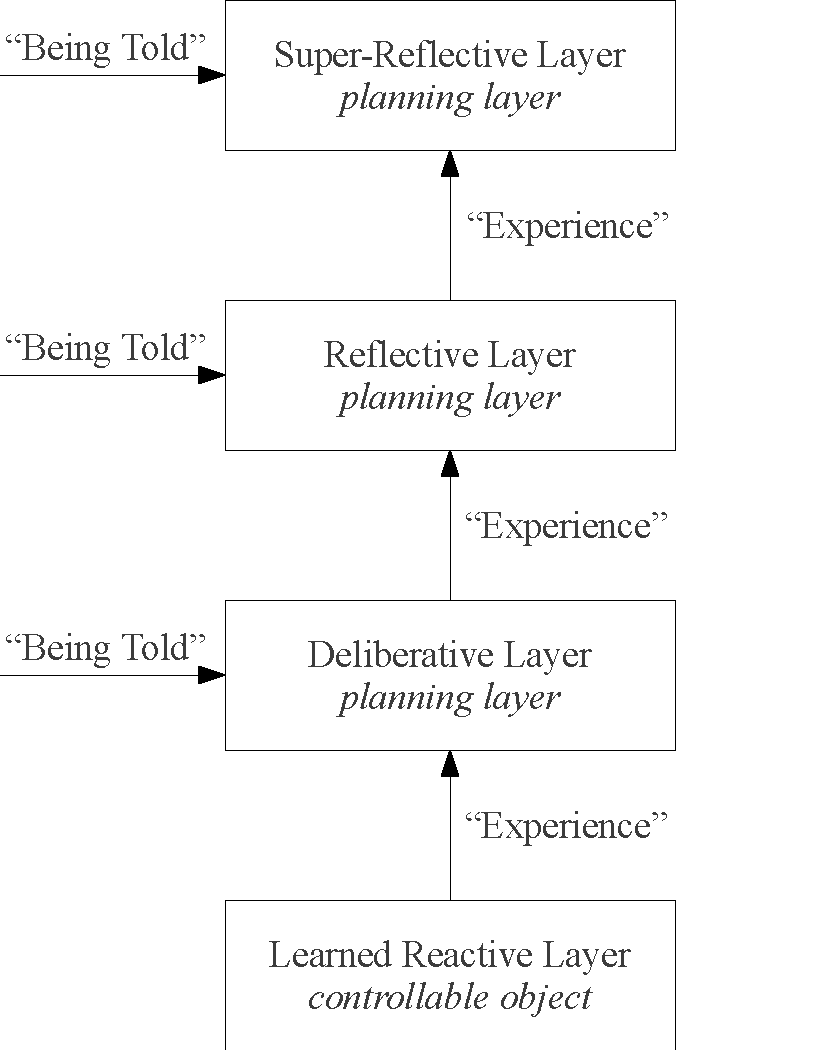
\includegraphics[width=6cm]{gfx/learning_from_being_told_in_layers}
\caption[Learning from being told and learning from experience both
  occur in each SALS planning layer.]{Learning from being told and
  learning from experience both occur in each SALS planning layer.
  When a layer of the AI learns from being told, a natural language
  plan is communicated to that layer from a source external to the AI,
  such as a human user.  When a layer of the AI learns from
  experience, two streams of trace events are received from the layer
  below that are asynchronously woven into hypothetical causal models
  of the effects of actions.}
\label{figure:learning_from_being_told_in_layers}
\end{figure}
In this chapter, I will focus on learning from being told natural
language plans.  I will describe the details of how each planning
layer in SALS asynchronously learns from experience in
{\mbox{\autoref{chapter:learning_asynchronously_from_experience}}}.
The important point that I will elaborate upon in this chapter is that
the SALS AI interprets natural language plans, while simultaneously
considering syntax, semantics, current environmental context, learned
hypothetical knowledge about the effects of actions as well as the
current positive and negative goals of the AI.  My approach is as
opposed to linguistic traditions that focus on only one or two of
these aspects of natural language understanding.

Natural language plans in SALS are in the form of a programming
language with variables, conditionals, recursion, ambiguous values, an
imaginative compiler, and the ability to use analogical patterns
between collections of these plans to interpret natural language
sentences and phrases.  SALS natural language plans are sequences of
commands that can be created, mutated, and executed by a planning
layer in order to accomplish goals.  The following is an example of a
definition of one of the deliberative plans that the AI in the story
could consider executing:
\begin{samepage}
\begin{Verbatim}
  [defplan 'move left'
    [call-below 'move left']]
\end{Verbatim}
\end{samepage}
This expression defines a new deliberative plan.  The
``{\tt{defplan}}'' command is shorthand for ``define plan.''  The
first argument to the defplan expression is the name of the plan:
``{\tt{move left}}.''  The body of the plan is the remaining sequence
of expressions.  The only expression in the body of this plan is the
``{\tt{call-below}}'' expression with the ``{\tt{move left}}''
argument.  This expression activates a resource in the layer below, in
this case, the ``{\tt{move left}}'' resource, which is in the built-in
reactive layer of the AI.  The ``{\tt{call-below}}'' expression not
only activates a resource in the layer below but also waits for that
resource to complete execution or fail.  The ``{\tt{move left}}'' plan
defines a possible natural language interpretation for the ``{\tt{move
    left}}'' phrase, stating that this phrase refers to the
synchronous execution of the ``{\tt{move left}}'' resource in the
layer below.

Consider this analogous plan to the ``{\tt{move left}}'' plan that
defines an interpretation of the ``{\tt{move right}}'' phrase:
\begin{samepage}
\begin{Verbatim}
  [defplan 'move right'
    [call-below 'move right']]
\end{Verbatim}
\end{samepage}
The analogous similarity between the ``{\tt{move left}}'' and
``{\tt{move right}}'' commands can be abstracted into a new
``{\tt{move left}}'' natural language plan that uses the following
syntax:
\begin{samepage}
\begin{Verbatim}
  [defplan 'move left'
    :matches ['move [? direction]']
     :frame [[direction 'left']]
      [call-below 'move [? direction]']]
\end{Verbatim}
\end{samepage}
This generalized form of the original ``{\tt{move left}}'' and
``{\tt{move right}}'' plans uses a natural language variable,
``{\tt{direction}}.''  Note that there are two optional arguments to
the defplan expression in this example: (1) ``{\tt{:matches}}'' and
(2) ``{\tt{:frame}}.''  The optional ``{\tt{:matches}}'' argument
specifies a list of potential natural language patterns that this plan
may match as it is being interpreted.  In this case, the variable
expression ``{\tt{[?  direction]}}'' is allowed to replace the word
``{\tt{left}}'' from the original name of the plan.  The optional
``{\tt{:frame}}'' argument specifies the default natural language
variable bindings.  In this case, the ``{\tt{direction}}'' variable is
assigned the natural language phrase ``{\tt{left}}'' by default.  In
the body of the generalized form of the plan, all occurrences of
``{\tt{left}}'' have been replaced with the variable expression
``{\tt{[?  direction]}}''.  Given this generalized form of the
original plan, the planner can create a new analogous plan as an
interpretation of either of the natural language phrases: ``{\tt{move
    left}}'' or ``{\tt{move right}}.''

\section{Conditionals and Partial States}

The SALS natural planning language includes conditional branches that
can change the course of plan execution based on the existence of
partial states in the knowledge base that it is trying to control.
For example, here is a more complicated SALS plan that shows a number
of new SALS primitives that will be discussed next:
\begin{samepage}
\begin{Verbatim}
  [defplan 'move toward a cube'
    [if [exists [relationship block property shape cube
	                      preposition left-of
	                      gripper property is-me true]]
        [call-below 'move left']
      [if [exists [relationship block property shape cube
                                preposition right-of
                                gripper property is-me true]]
          [call-below 'move right']
        [fail]]]]
\end{Verbatim}
\end{samepage}
This plan checks to see if there is a cube to the left of the gripper
that the AI is controlling.  If there is a cube to the left, this plan
will activate the ``{\tt{move left}}'' resource in the layer below.
If there is not a cube to the left, this plan then checks to see if
there is a cube to the right of the gripper that the AI is
controlling.  If there is a cube to the right, this plan will activate
the ``{\tt{move right}}'' resource in the layer below.  At this point,
if there is not a cube to the left or to the right, the plan fails.
There are a number of new primitives that are introduced in this
example of conditional branches:
\begin{packed_itemize}
\item{``{\tt{if}}''}
\item{``{\tt{exists}}''}
\item{``{\tt{relationship}}''}
\item{``{\tt{fail}}''}
\end{packed_itemize}
The syntax for the SALS ``{\tt{if}}'' expression is similar to the
``{\tt{if}}'' expression in most lisp-like languages: the first
argument is the conditional, the second argument is the true branch,
and the remaining arguments are the optional body of the false branch.
Unlike most lisp-like languages, the SALS ``{\tt{if}}'' expression's
conditional value must be a Boolean type object and will fail with any
other value.  The ``{\tt{fail}}'' expression is a simple way for a
plan to stop executing and mark the plan with the knowledge of a
failure object.  The ``{\tt{exists}}'' expression accepts a partial
state as its only argument and checks to see if this partial state
exists in the knowledge base that the planning layer is trying to
control.  When the effects of a plan are being imagined, the return
value of the ``{\tt{exists}}'' expression are not known, so multiple
possible ambiguous values are returned: (1) the result based on
current hypothetical models of the effects of previous actions or the
current state of the knowledge base that this planning layer is trying
to control if no previous actions have been imagined, (2) a true value
based on the possibility that learned models are incorrect, and (3) a
false value based on the possibility that learned models are
incorrect.  The ``{\tt{relationship}}'' expression is one of two
special expressions in SALS that return partial state objects.  The
``{\tt{relationship}}'' expression accepts ten arguments, which map
directly to the internal semantic graph representation of the
knowledge base that the planning layer is trying to control.  The
following are the ten arguments to the ``{\tt{relationship}}''
expression:
\begin{packed_enumerate}
\item{{\tt{source-type}}}
\item{{\tt{source-key-type}}}
\item{{\tt{source-key}}}
\item{{\tt{source-value}}}
\item{{\tt{key-type}}}
\item{{\tt{key}}}
\item{{\tt{target-type}}}
\item{{\tt{target-key-type}}}
\item{{\tt{target-key}}}
\item{{\tt{target-value}}}
\end{packed_enumerate}
{\mbox{\autoref{figure:relationship_partial_state_graph}}} shows how
the arguments to the ``{\tt{relationship}}'' expression map to the
frame types, slot values, and properties of a frame-based knowledge
base that is represented as a graph.  When an argument to the
``{\tt{relationship}}'' expression is a symbol, this symbol is checked
against a list of known symbols within the SALS AI.  If an argument to
the ``{\tt{relationship}}'' expression is not a known symbol, this
results in an interpretation failure, limiting the number of possible
interpretations.
\begin{figure}
\centering
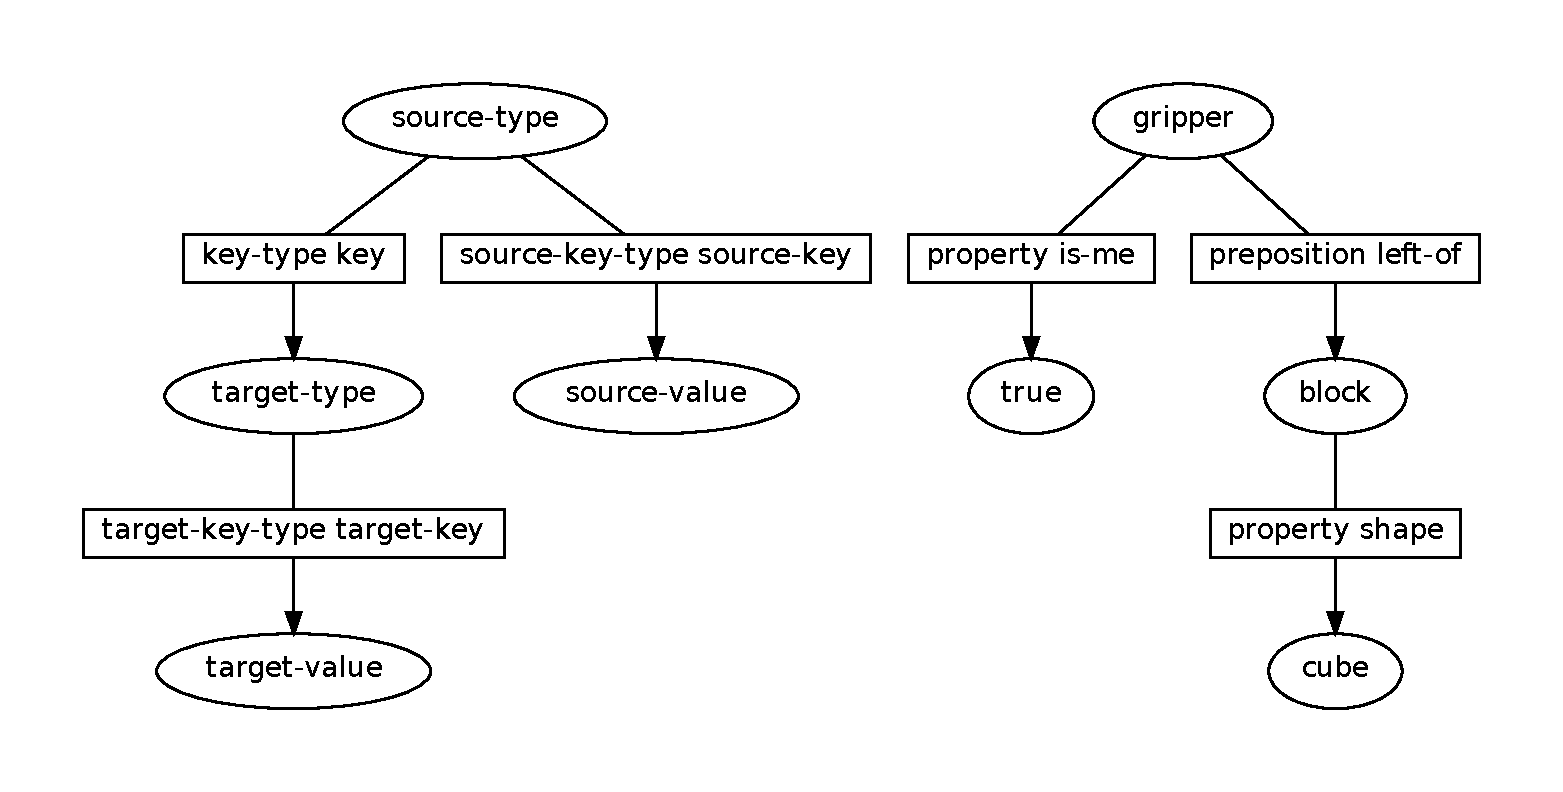
\includegraphics[width=12cm]{gfx/relationship_partial_state_graph}
\caption[The SALS ``{\tt{relationship}}'' expression returns a partial
  state object.]{The SALS ``{\tt{relationship}}'' expression returns a
  partial state object.  The graph on the left shows the ten argument
  names for the ``{\tt{relationship}}'' expression, while the graph on
  the right shows a potential partial state of the physical knowledge
  base that literally means, ``{\tt{a cube shaped block to be to the
      left of a gripper that is me}}.''}
\label{figure:relationship_partial_state_graph}
\end{figure}

Now, let us consider a slightly different type of partial state
expression in the following example plan that attempts to control the
gripper to grab a block:
\begin{samepage}
\begin{Verbatim}
  [defplan 'attempt to grab block'
    [call-below 'grab']
    [wait-for [property gripper property is-me true
                        property movement-command
                        stop]]]
\end{Verbatim}
\end{samepage}
In this plan, two new types of SALS expressions are introduced:
\begin{packed_itemize}
\item{``{\tt{wait-for}}''}
\item{``{\tt{property}}''}
\end{packed_itemize}
The ``{\tt{wait-for}}'' expression takes one argument, which similarly
to the ``{\tt{exists}}'' expression, must be a partial state object,
such as that returned by the ``{\tt{relationship}}'' expression.
Functionally, the ``{\tt{wait-for}}'' expression puts the plan to
sleep until the specified partial state exists in the knowledge base
in the layer below that this plan is trying to control.  The
``{\tt{property}}'' expression is similar to the
``{\tt{relationship}}'' expression in that it does return a partial
state object, but the ``{\tt{property}}'' expression only takes the
following seven arguments:
\begin{packed_enumerate}
\item{{\tt{source-type}}}
\item{{\tt{source-key-type}}}
\item{{\tt{source-key}}}
\item{{\tt{source-value}}}
\item{{\tt{key-type}}}
\item{{\tt{key}}}
\item{{\tt{value}}}
\end{packed_enumerate}
{\mbox{\autoref{figure:relationship_partial_state_graph}}} shows how
the arguments to the ``{\tt{property}}'' expression map to the frame
types, slot values, and properties of a frame-based knowledge base
that is represented as a graph.
\begin{figure}
\centering
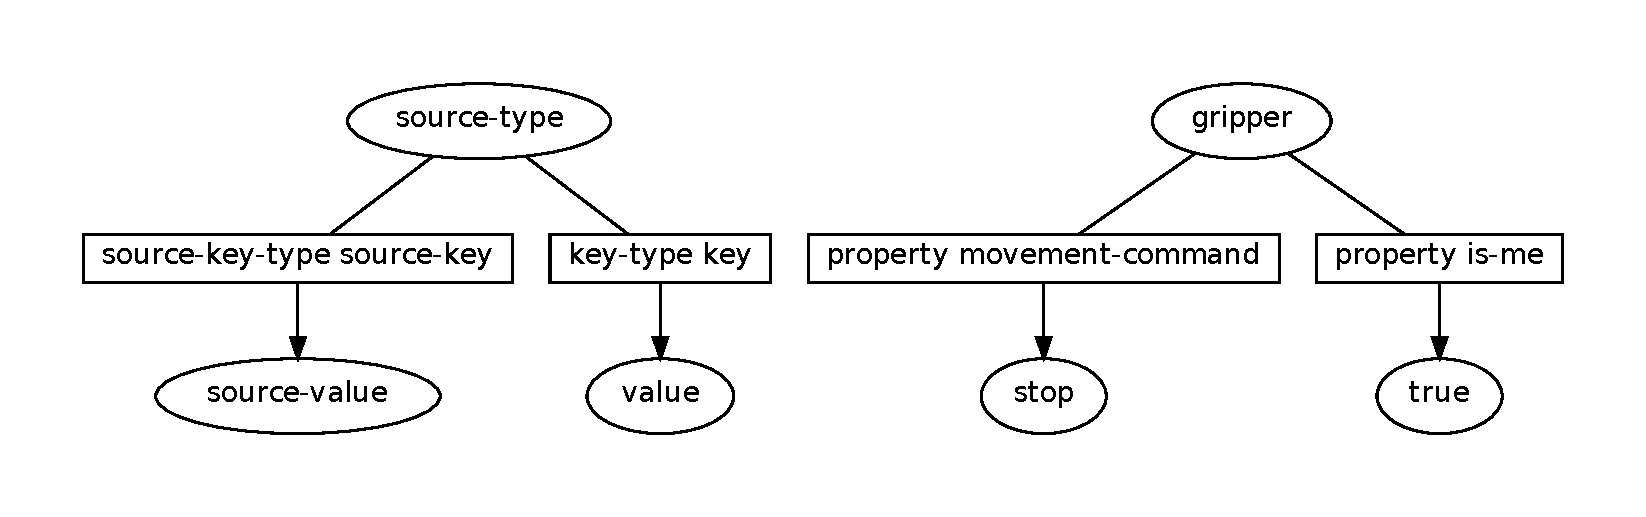
\includegraphics[width=12cm]{gfx/property_partial_state_graph}
\caption[The SALS ``{\tt{property}}'' expression returns a partial
  state object.]{The SALS ``{\tt{property}}'' expression returns a
  partial state object.  The graph on the right shows the seven
  argument names for the ``{\tt{property}}'' expression, while the
  graph on the left shows a potential partial state of the physical
  knowledge base that literally means, ``{\tt{a gripper to be me and
      have a stop movement command}}.''}
\label{figure:property_partial_state_graph}
\end{figure}

While the deliberative layer may create plans that refer to partial
states in the physical knowledge base, the reflective layer may create
plans that refer to partial states in the deliberative plan knowledge
base, which may in turn also refer to partial states in the physical
knowledge base.  Consider the following example of a reflective plan
that includes this form of hierarchical partial state reference:
\begin{samepage}
\begin{Verbatim}
  [defplan 'a deliberative planner to have a positive goal
            for a cube to be on a pyramid'
    [property planner property layer deliberative
              property positive-goal
              [relationship block property shape cube
                            preposition on
                            block property shape pyramid]]]
\end{Verbatim}
\end{samepage}
In this reflective plan, the ``{\tt{property}}'' expression describes
a partial state of the deliberative plan knowledge base, while the
``{\tt{relationship}}'' expression describes a partial state of the
physical knowledge base.  In order for SALS to convert this expression
to a purely deliberative form of knowledge, hierarchical partial
states are reified in SALS so that they become a simple partial state
that is purely of one layer's type of knowledge.  When a partial state
object is passed as an argument to another partial state object, the
first partial state is converted to a symbolic form, so that the
entire structure can continue to exist as a simple frame-based graph
structure.  {\mbox{\autoref{figure:hierarchical_partial_state_graph}}}
shows an example of a hierarchical embedding of
``{\tt{relationship}}'' and ``{\tt{property}}'' partial states that
may occur in any planning layer above the deliberative layer.
\begin{figure}
\centering
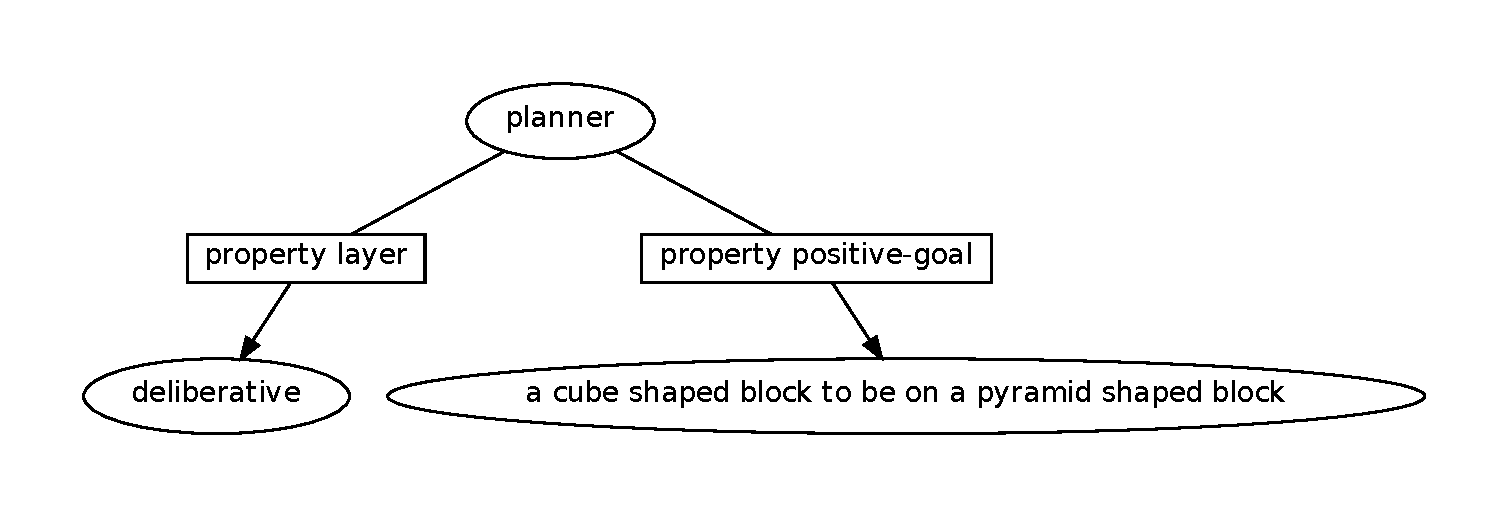
\includegraphics[width=12cm]{gfx/hierarchical_partial_state_graph}
\caption[The SALS ``{\tt{relationship}}'' and ``{\tt{property}}''
  expressions can be hierarchically combined in planning layers above
  the deliberative.]{The SALS ``{\tt{relationship}}'' and
  ``{\tt{property}}'' expressions can be hierarchically combined in
  planning layers above the deliberative.  Note that any partial
  states that are sub-expressions of other partial states become
  symbolically reified in order to maintain a frame-based graph
  structure for all knowledge.}
\label{figure:hierarchical_partial_state_graph}
\end{figure}

\section{Plans Interpreting Plans}
\label{section:plans_interpreting_plans}

The most powerful capability of the SALS natural language programming
language is the ability to find correct interpretations of ambiguous
natural language plans.  Let us first define the following simple
natural language plan that returns a ``{\tt{relationship}}'' partial
state object:
\begin{samepage}
\begin{Verbatim}
  [defplan 'a cube to be to my left'
    [relationship block property shape cube
                  preposition left-of
                  gripper property is-me true]]
\end{Verbatim}
\end{samepage}
This plan can be generalized to analogously work for any type of shape
as in the following example:
\begin{samepage}
\begin{Verbatim}
  [defplan 'a cube to be to my left'
    :matches ['a [? shape] to be to my left']
     :frame [[shape 'cube']]
      [relationship block property shape [? shape]
                    preposition left-of
                    gripper property is-me true]]
\end{Verbatim}
\end{samepage}
Now, consider the following plan that makes use of this previous plan
definition and introduces two new SALS expression types for evaluating
natural language plans:
\begin{samepage}
\begin{Verbatim}
  [defplan 'a cube is to my left'
    [exists [plan-call [plan 'a cube to be to my left']]]]
\end{Verbatim}
\end{samepage}
This last plan returns a true or false value depending on whether or
not the partial state returned by the plan, ``{\tt{a cube to be to my
    left}},'' exists in the knowledge base that the planning layer is
trying to control.  Two new types of SALS natural language programming
expressions are introduced in the last plan:
\begin{packed_enumerate}
\item{``{\tt{plan-call}}''}
\item{``{\tt{plan}}''}
\end{packed_enumerate}
The ``{\tt{plan}}'' expression takes one argument, a natural language
phrase.  The ``{\tt{plan}}'' expression returns a plan from the
current planning layer that matches the given natural language phrase.
If there is no matching natural language plan, SALS will attempt to
find an plan that has an analogous match to the given natural language
phrase.  In most cases, there are multiple possible matches for any
given natural language phrase.  In these cases, the SALS natural
language plan compiler is responsible for imagining the effects of
different interpretations on the knowledge base that the planning
layer is trying to control, while avoiding natural language plan
interpretation failures.  The ``{\tt{plan-call}}'' expression accepts
one argument, a natural language subplan to compile into this location
of the current plan that is being defined by the ``{\tt{defplan}}''
expression.

Now, consider the following redefinition of the previous ``{\tt{move
    toward a cube}}'' plan that I defined previously:
\begin{samepage}
\begin{Verbatim}
  [defplan 'move toward a cube'
    [if [plan-call [plan 'a cube is to my left']]
        [call-below 'move left']
      [if [plan-call [plan 'a cube is to my right']]
          [call-below 'move right']
        [fail]]]]
\end{Verbatim}
\end{samepage}
This version of the ``{\tt{move toward a cube}}'' natural language
plan is simpler because it only indirectly references the
``{\tt{relationship}}'' and ``{\tt{exists}}'' expressions through the
``{\tt{plan}}'' and ``{\tt{plan-call}}'' expressions that refer to the
appropriate analogies to other natural language plans.  Now, consider
the following expression that defines an analogy for any natural
language plans that use the ``{\tt{if}}'' expression:
\begin{samepage}
\begin{Verbatim}
  [defplan 'if a cube is to my left, move left,
            otherwise move right'
    :matches ['if [? condition], [? true-branch],
               otherwise [? false-branch]']
     :frame [[condition    'a cube is to my left']
             [true-branch  'move left']
             [false-branch 'move right']]
      [if [plan-call [plan [? condition]]]
          [plan-call [plan [? true-branch]]]
        [plan-call [plan [? false-branch]]]]]
\end{Verbatim}
\end{samepage}
Using this definition of an analogy for the ``{\tt{if}}'' expression,
the original ``{\tt{move toward a cube}}'' natural language plan can
be rewritten as follows:
\begin{samepage}
\begin{Verbatim}
  [defplan 'move toward a cube'
    [plan-call [plan 'if a cube is to my left, move
                      left, otherwise if a cube is
                      to my right, move right,
                      otherwise fail']]]
\end{Verbatim}
\end{samepage}
Note that this last plan uses two ``{\tt{if}}'' statements, the second
is in the false branch of the first.

Before getting to the details of how ambiguity in searched through and
eliminated in the SALS natural language plan compiler, consider the
following definitions that include the SALS ``{\tt{not}}'' expression:
\begin{samepage}
\begin{Verbatim}
  [defplan 'a cube is not to my left'
    [not [plan-call [plan 'a cube is to my left']]]]
\end{Verbatim}
\end{samepage}
The SALS ``{\tt{not}}'' expression is similar to the ``{\tt{not}}''
expression in most lisp-like programming languages in that it takes
one argument.  Unlike most lisp-like languages, the SALS
``{\tt{not}}'' expression only accepts a Boolean type of object.  The
``{\tt{not}}'' expression returns a new Boolean type object that
represents the opposite value of the argument.  The following is an
analogous plan that can be used to generalize this natural language
usage of the ``{\tt{not}}'' expression:
\begin{samepage}
\begin{Verbatim}
  [defplan 'a cube is not to my left'
    :matches ['[? subject] is not [? preposition]']
     :frame [[subject     'a cube']
             [preposition 'to my left']]
      [not [plan-call [plan '[? subject] is
                             [? preposition]']]]]
\end{Verbatim}
\end{samepage}
This plan allows many negative expressions to analogously have a
correct interpretation, such as ``{\tt{if a pyramid is not to my
    right, move left, otherwise fail}}.''

Another powerful component of the SALS natural programming language is
the ability to compile natural language plans that include recursive
references, which enable plans to describe looping functionality.
SALS also has a primitive capability to imagine the possible effects
of loops by imaginatively unrolling the loop only once.  The following
example is a definition of a reflective natural language plan that
searches for a deliberative plan whose effects have not yet been
imagined:
\begin{samepage}
\begin{Verbatim}
  [defplan 'find next unimagined plan'
    [call-below 'focus on next object']
    [plan-call [plan 'if a planner is focusing on
                      a plan that has been imagined,
                      find next unimagined plan']]]
\end{Verbatim}
\end{samepage}
Notice that the name of this plan is ``{\tt{find next unimagined
    plan}},'' which is the same as the true branch of the natural
language ``{\tt{if}}'' statement in the body of the plan.  This plan
checks to see if the plan currently in the focus of the deliberative
planner has been imagined.  If the plan in deliberative focus has been
imagined, this plan calls itself recursively until the deliberative
planner is focusing on a plan that has not been imagined.

As a final example of a natural language plan interpreting a natural
language plan, consider again the following hierarchical partial state
construction from a reflective natural language plan from earlier in
this chapter:
\begin{samepage}
\begin{Verbatim}
  [defplan 'a deliberative planner to have a positive goal
            for a cube to be on a pyramid'
    [property planner property layer deliberative
              property positive-goal
              [relationship block property shape cube
                            preposition on
                            block property shape pyramid]]]
\end{Verbatim}
\end{samepage}
This reflective natural language plan can be abstracted with
``{\tt{plan}}'' and ``{\tt{plan-call}}'' expressions as in the
following example:
\begin{samepage}
\begin{Verbatim}
  [defplan 'a deliberative planner to have a positive goal
            for a cube to be on a pyramid'
    :matches ['a deliberative planner to have a positive
               goal for [? partial-state]']
     :frame [[partial-state 'a cube to be on a pyramid']]
      [property planner property layer deliberative
                property positive-goal
                [plan-call [plan [? partial-state]]]]]
\end{Verbatim}
\end{samepage}
In this way, analogous reflective plans can be created in order to
allow the interpretation of any natural language physical partial
state being a positive goal of the deliberative planning layer.  A
similar technique can be used to create analogous reflective natural
language plans that work for negative goals as well as plans that are
hypothesized to cause partial states to exist.

\section{Analogous Plan Interpretation}

As previously described, the ``{\tt{plan}}'' expression in a SALS
natural language plan returns a plan object that either matches the
name of a plan previously defined via the ``{\tt{defplan}}''
expression, or if an analogy can be found to an existing plan, a new
analogous plan object is created and returned as the result of the
``{\tt{plan}}'' expression.  Because of the possibility that multiple
plans may match a given ``{\tt{plan}}'' expression, it is the task of
the SALS compiler to imagine the effects of the different
interpretations and decide upon one for execution.  The SALS natural
language plan compiler must handle multiple ambiguous return values
for each ``{\tt{plan}}'' expression.  Let us consider again the
following natural language plan that must be imagined and interpreted,
which requires the compiler to sort through multiple possible
interpretations:
\begin{Verbatim}
  [plan-call [plan 'if a cube is not on a pyramid, stack a
                    cube on a pyramid']]
\end{Verbatim}
A reasonable way to expect this natural language phrase to be
interpreted is as a plan analogous to the natural language plan for
the ``{\tt{if}}'' expression similar to the one previously defined, as
in the following:
\begin{samepage}
\begin{Verbatim}
  [defplan 'if a cube is not on a pyramid, stack a cube on a
            pyramid'
    :matches ['if [? condition], [? true-branch]']
     :frame [[condition    'a cube is not on a pyramid']
             [true-branch  'stack a cube on a pyramid']]
      [if [plan-call [plan [? condition]]]
          [plan-call [plan [? true-branch]]]]]
\end{Verbatim}
\end{samepage}
Although this plan makes sense, there are many other possible
problematic analogies to previously defined natural language plans
that do not make any sense at all.  The following problematic
interpretation is one example:
\begin{samepage}
\begin{Verbatim}
  [defplan 'if a cube is not on a pyramid, stack a cube on a
            pyramid'
    :matches ['[? subject] is not [? preposition]']
     :frame [[subject     'if a cube']
             [preposition 'on a pyramid, stack a cube on a
                           pyramid']]
      [not [plan-call [plan '[? subject] is
                             [? preposition]']]]]
\end{Verbatim}
\end{samepage}
Notice that the natural language value of the ``{\tt{subject}}''
variable in the previous problematic interpretation is equal to
``{\tt{if a cube}}.''  The following is the result of one step in
compiling this problematic interpretation:
\begin{Verbatim}
  [not [plan-call [plan 'if a cube is on a pyramid, stack a
                         cube on a pyramid']]]
\end{Verbatim}
Notice that the ``{\tt{not}}'' expression has been moved to the front
of this expression after it has been partially compiled.  The
following is the result of another couple steps of further
interpreting the remaining natural language in this expression:
\begin{Verbatim}
  [not [if [exists [plan-call [plan 'a cube to be on a
                                     pyramid']]]
           [plan-call [plan 'stack a cube on a pyramid']]]]
\end{Verbatim}
When this problematic interpretation is imagined, the result from the
``{\tt{exists}}'' expression is a Boolean value, so this satisfies the
``{\tt{if}}'' conditional type requirement.  However, the result of
the ``{\tt{if}}'' expression is the special type ``{\tt{nil}},'' which
is not a Boolean value in the SALS natural programming language.
Because the ``{\tt{not}}'' expression strictly requires a Boolean type
value, the imaginative interpretation of this plan fails when the nil
value from the ``{\tt{if}}'' statement reaches the ``{\tt{not}}''
expression.  Using strict typing in the low-level details of the SALS
natural programming language allows ambiguous high-level expressions
with many possible interpretations to be narrowed down to a few that
make programmatic sense.  By introducing more constraints to the
low-level details of the SALS natural programming language, many types
of plan failures can be imagined and avoided, even while using this
very loose type of natural language analogical matching technique.
Not all errors can be imagined and avoided through imaginative
compiling, but many types of failures are avoided in this way.
However, some failures, such as expectation failures, can only be
realized during the actual execution of the plan.

\section{Imagining the Effects of Ambiguous Plans}
\label{section:imagining_the_effects_of_ambiguous_plans}

As natural language plans are interpreted, the hypothetical effects of
any resource activations in the layer below are also simultaneously
imagined in the counterfactual knowledge base of that planning layer.
Imagining the effects of resource activations first requires that
hypothetical models of the effects of resource activations exist.
Hypothetical models of the effects of resource activations in SALS
provide a rule-based mapping from the preconditions of the resource
activation to the potential transframes for the resource activation.
The preconditions and transframes are in terms of the abstract partial
states that have previously existed in the knowledge base that the
planning layer is trying to control.  For example, ``{\tt{a gripper
    that is me being above a cube shaped block}}'' could be one of
many preconditions for an action.  All partial states that can be
returned by the ``{\tt{relationship}}'' and ``{\tt{property}}''
expressions in the SALS natural programming language are efficiently
abstracted asynchronously from the knowledge base that the planning
layer is trying to control.  I will describe the details of the
abstract asynchronous learning algorithm for each planning layer in
{\mbox{\autoref{chapter:learning_asynchronously_from_experience}}}.
For now, know that abstract hypothetical models of resource
activations are learned and can be used for imagining the effects of
resource activations during the natural language plan interpretation
process.

Because some expressions in the SALS natural planning language can
return multiple possible ambiguous values, one task of the planning
layer is to decide which of the multiple possible interpretations is
complete, accomplishes positive goals and avoids negative goals.  This
means that each expression in the SALS natural programming language
may have one or more possible different outcomes, depending on the
interpretation path and which one of potentially multiple ambiguous
values is chosen to be executed when a decision must be made.  In
order to keep track of each of these different interpretations, each
plan expression is allocated an {\emph{execution node}} object and
each decision among multiple ambiguous argument values is allocated an
{\emph{argument decision node}} object in the plan knowledge base of
that planning layer.  The execution node objects correspond to the
functional hierarchy of the imagined natural language plan execution,
while the argument decision node objects represent any points in the
imagined execution where two potentially different sub-trees of the
functional execution could occur based on different choices between
multiple possible ambiguous return values from sub-expressions of the
current expression being imaginatively executed.
\begin{figure}
\hspace*{-1cm}\includegraphics[width=14cm]{gfx/plan_execution_node_graph}
\caption[A graph representation of the deliberative plan knowledge
  base while a simple plan with multiple ambiguous interpretations is
  being imaginatively interpreted and evaluated.]{A graph
  representation of the deliberative plan knowledge base while a
  simple plan with multiple ambiguous interpretations is being
  imaginatively interpreted and evaluated.  The deliberative
  {\emph{planner}} object is focusing on a {\emph{plan}} object that
  has been partially evaluated.  The first execution node object of
  this plan object represents the partial interpretation of a
  ``{\tt{not}}'' expression that has a ``{\tt{plan-call}}''
  sub-expression.  The ``{\tt{plan}}'' expression returns two possible
  values, which are interpreted separately under argument decision
  node objects.}
\label{figure:plan_execution_node_graph}
\end{figure}
{\mbox{\autoref{figure:plan_execution_node_graph}}} shows a graph
representation of the frame-based deliberative plan knowledge base as
it is in the process of imaginatively evaluating the following simple
plan:
\begin{samepage}
\begin{Verbatim}
  [defplan 'a cube is not on a pyramid'
    :matches ['[? subject] is not [? preposition]']
     :frame [[subject     'a cube']
             [preposition 'on a pyramid']]
      [not [plan-call [plan '[? subject] is
                             [? preposition]']]]]
\end{Verbatim}
\end{samepage}
When this natural language plan is imaginatively interpreted, there
are multiple possible values returned from the ``{\tt{plan}}''
expression, which returns analogous plans that match the natural
language phrase, ``{\tt{a cube is on a pyramid}}.''  In this case,
there are the two following plans that are created as analogies to
other known plans:
\begin{packed_enumerate}
\item{
\begin{samepage}
\begin{Verbatim}
  [defplan 'a pyramid is on a cube'
    :matches ['a [? top-shape] is on a [? bottom-shape]']
     :frame [[top-shape    'pyramid']
             [bottom-shape 'cube']]
      [exists [relationship block property shape
                              [? top-shape]
                            preposition on
                            block property shape
                              [? bottom-shape]]]]
\end{Verbatim}
\end{samepage}
}
\item{
\begin{samepage}
\begin{Verbatim}
  [defplan 'a pyramid is on a cube'
    :matches ['a [? top-color] is on a [? bottom-color]']
     :frame [[top-color    'pyramid']
             [bottom-color 'cube']]
      [exists [relationship block property color
                              [? top-color]
                            preposition on
                            block property color
                              [? bottom-color]]]]
\end{Verbatim}
\end{samepage}
}
\end{packed_enumerate}
The first of these two analogous interpretations is what one would
expect: the natural language phrases ``{\tt{pyramid}}'' and
``{\tt{cube}}'' are interpreted to be shapes of blocks that are on top
of one another.  The second of these interpretations is less obvious
and incorrectly interprets ``{\tt{pyramid}}'' and ``{\tt{cube}}'' to
be colors.  This problematic interpretation is an analogy to the
following plan that the SALS AI already knows:
\begin{samepage}
\begin{Verbatim}
  [defplan 'a red is on a blue'
    :matches ['a [? top-color] is on a [? bottom-color]']
     :frame [[top-color    'red']
             [bottom-color 'blue']]
      [exists [relationship block property color
                              [? top-color]
                            preposition on
                            block property color
                              [? bottom-color]]]]
\end{Verbatim}
\end{samepage}
The SALS AI does not immediately know that ``{\tt{red}}'' and
``{\tt{blue}}'' are colors, while ``{\tt{cube}}'' and
``{\tt{pyramid}}'' are shapes.  While types of partial states could be
programmed into the SALS AI so that these specific words could be
assigned specific symbolic types, this is not the approach taken in
the SALS AI.  Instead, both of these interpretations are plausible in
the SALS AI.  However, when the SALS AI does finish imagining all
possible interpretations of a natural language phrase, each different
resulting analogous plan has a set of associated hypothetical states
that this plan may or may not accomplish.  If the possible effects of
a plan include a ``{\tt{pyramid}}'' color, which does not make sense,
the SALS AI sees that this is not one of its goals, so it ignores this
interpretation for that reason alone.  The SALS AI is a goal-oriented
natural language understanding system in this sense---finding those
natural language plan interpretations that it thinks will accomplish
its positive goals.  On the other hand, the SALS AI considers its
negative goals in the opposite sense: when a natural language plan
interpretation is hypothesized to accomplish a negative goal, that
plan interpretation is ignored.  The SALS AI can be considered to be
an ``optimistic'' or ``pessimistic'' natural language understanding
system in these cases.  The important point here is that the SALS AI
interprets natural language plans, while simultaneously considering
syntax, semantics, current environmental context, learned hypothetical
knowledge about the effects of actions as well as the current positive
and negative goals of the AI.

There are two ways that a natural language plan is hypothesized to
cause a specific partial state: (1) learned hypothetical models are
used to predict the effects of actions, and (2) existence checks for
partial states during the imaginative interpretation of the plan are
used as secondary evidence that a plan may or may not be expecting a
specific partial state to exist during its execution.  For example, if
a natural language plan checks for the existence of the partial state,
``{\tt{a cube shaped block to be on top of a pyramid shaped block}},''
this existence check provides secondary evidence that this plan could
be expecting this state to exist during its execution.  This secondary
evidence of the possible intentions of a plan is an example of
knowledge learned during the imaginative interpretation of natural
language plans in the SALS AI.


\mymargins
%************************************************
\chapter{Learning Asynchronously from Experience}
\label{chapter:learning_asynchronously_from_experience}
%************************************************

\section{Representing Actions}

The planning as search problem assumes that we have a representation
of the world and a representation for the changes that actions
perform.  Given these models, the physical world can be simulated
according to different plans.  \cite{fikes:1972} describe an action
representation, called ``STRIPS'', that includes an \emph{add list}
and a \emph{delete list} to represent the change between states in the
world.  In the STRIPS model, the world is a set of symbols.  A
transframe is composed of two sets: one for the removals from the
world and one for the additions to the world.

An object called a \emph{frame transition} \cite[]{minsky:1975} or a
\emph{transframe} \cite[]{minsky:1988} is similar to a STRIPS operator
with add and delete lists but that is also able to simulate actions in
frame-based and other relational domains.  A transframe represents a
change between two relational states of the world.  In a symbolic
relational domain, the state space is a set of symbolic relationships
rather than just symbols.  Here is an example of a symbolic
relationship that could exist in a relational domain: {\tt [block-1
    is-on block-2]}.  Here is an example of a transframe for the world
in a relational domain: \emph{delete} {\tt [block-1 on table-1]} and
\emph{add} {\tt [block-1 on block-2]}.  In predicting the effects of
an action on the world, STRIPS considers one transframe for each
action.

Transframes can also be dependent on the current state of the world.
Although many function approximation methods could be used, in my
simulation model I have addressed the problem of learning to predict
the correct transframes in the terms of
{\mbox{\citeauthor{mitchell:1997}'s~\citeyearpar{mitchell:1997}}}
``hypothesis spaces,'' which provide a simple and understandable
formulation of the category hypothesis learning problem, given
labelled examples.  Hypothetical models are learned to predict the
effects of actions.  The physical state space informs sets of
hypotheses that can be used to support assumptions, thus, the creation
of new knowledge from an absence of knowledge, given the listed
assumptions.






\section{Old Beginning}

Hypothetical type knowledge transframes are used by the deliberative
and reflective planning machines in order to infer the effects of
executing plans.  There is a distinction here made between the
\emph{factual} knowledge that is directly an abstraction of knowledge
grounded in the physical or deliberative planning machine knowledge
bases, which are not based on any learned action hypotheses, and the
\emph{counterfactual} knowledge that is inferred and supported by
hypotheses of the effects of resource executions that the AI has
either ``been told'' or has learned in the course of actually
executing those resources in different contexts.  In order to maintain
this distinction in the AI, different knowledge bases are used to
separate the factual knowledge from counterfactual knowledge.  Factual
knowledge is induced into factual type knowledge abstractions.  The
factually grounded knowledge bases include the visual, physical,
physical type, deliberative planning machine, and deliberative
planning machine type knowledge bases.  However, the addition of
factually grounded knowledge causes a loss of hypotheses from the
resource execution type knowledge transframe hypothesis spaces in both
the deliberative and reflective layers.  Each counterfactual event in
the counterfactual knowledge bases has a list of dependencies that
must maintain their support in order for the counterfactual knowledge
to continue to exist.  Dependencies in the AI have three types of
support that can be rearranged in order to maintain the support of
counterfactual knowledge events:
\begin{enumerate}
\item Resource execution transframe preconditions.
\item Resource execution.
\item Resource execution transframe change hypotheses.
\end{enumerate}
If any of these three types of supports loses its hypothetical factual
grounding, this loss of hypothetical factual grounding causes the
dependency to become \emph{invalidated}.  Once a dependency has become
invalidated, it has a chance to find new hypothetical grounding before
it becomes \emph{unsupported}.  Counterfactual event knowledge is
notified when a dependency has become unsupported, causing the
counterfactual events to be removed from the counterfactual event
knowledge bases.  Also, as some counterfactual knowledge may form
hypothetical grounding for further dependencies of further
counterfactual event knowledge, the loss of support for a dependency
can cause a chain reaction through events and the dependencies that
rely on these events for grounding.  In this way, additional factual
knowledge refines and reduces the hypothetical support of transframe
changes, invalidating hypothetical dependencies, and potentially
causing the loss of support for counterfactual knowledge that has been
inferred in the counterfactual event knowledge bases of the
deliberative and reflective layers of the AI.

\section{Learning from Being Told Deliberative Plans}

In {\mbox{\autoref{table:a_plan_learned_from_being_told}}} on page
{\mbox{\pageref{table:a_plan_learned_from_being_told}}}, there is an
assertion at the end of the plan for reactive resource execution that
the AI has been told: ``Assert a cube is sitting on a pyramid.''  When
the AI initially learns a plan from being told, it does not yet have
any factual knowledge to eliminate any hypotheses about the effects of
the resource executions.  When the AI learns plan knowledge from being
told, the asserted type knowledge in the plan are added to the
resource execution hypothesis spaces before the assertion.  In this
case, the resource execution immediately before the assertion is:
``Drop and wait for block to fall.''  Therefore, the AI does not
eliminate any hypotheses from the resource execution hypothesis spaces
but instead augments the potential \emph{change features} of this
resource's hypothesis spaces with this new \emph{add} change.  In
other words, the hypothesis space for the resource execution is
augmented to include all consistent hypotheses that both predict this
change and that do not predict this change.  Since the AI has no
previous factual knowledge about this change, it is capable of
predicting both possibilities, each with different sets of supporting
hypotheses: (1) that this feature is added when the resource is
executed in the given preconditions or (2) that this feature is not
added in the given preconditions.
{\mbox{\autoref{figure:inference_of_physical_knowledge}}} shows how
the augmented hypothesis space of this resource execution causes the
imaginative inference that will result in the future counterfactual
knowledge: ``A cube is sitting on a pyramid.''  Also, notice how the
three different types of dependencies relate the factual physical type
knowledge to this counterfactual physical type knowledge through the
potential reactive resource execution in order to predict the
hypothetically supported stack of blocks in the future.
\begin{figure}[h]
\centering
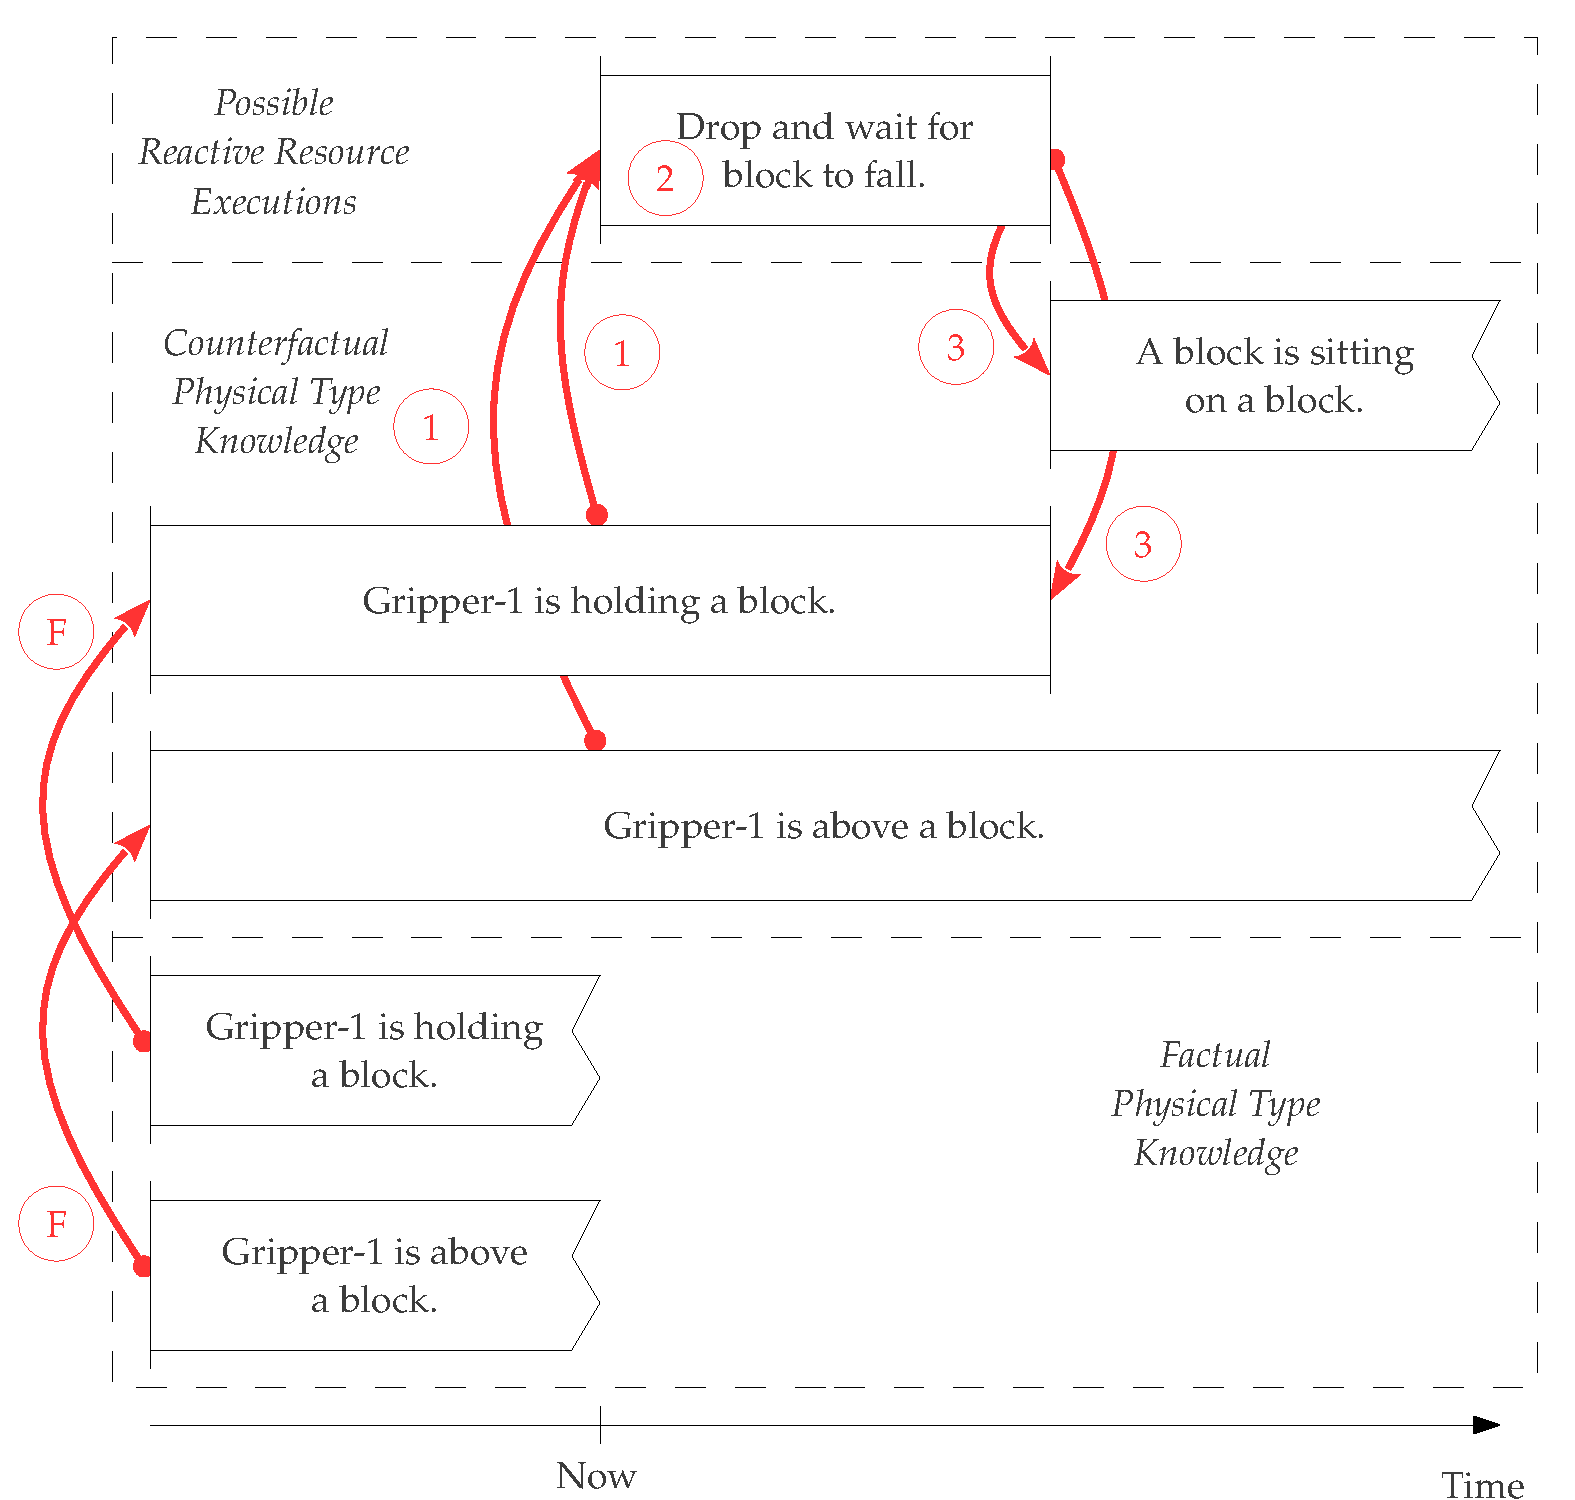
\includegraphics[width=12cm]{gfx/inference_of_physical_knowledge}
\caption[Inference of counterfactual physical type knowledge from
  factual physical type knowledge.]{Inference of counterfactual
  physical type knowledge from factual physical type knowledge.
  Rectangular boxes represent events over time.  Some events have a
  jagged right edge to indicate that this event has no ending time.
  Curved arrows represent different dependency relationships: (F)
  factual, (1) precondition, (2) potential resource execution, and (3)
  hypothetical change.  Preconditions, potential resource activations,
  and hypothetical changes form the three possibly unsupported parts
  of a dependency.  Factual dependencies cannot lose support because
  they are derived directly from factual events.}
\label{figure:inference_of_physical_knowledge}
\end{figure}
{\mbox{\autoref{figure:inference_of_deliberative_planning_machine_knowledge}}}
shows how the three different types of dependencies analogously relate
factual deliberative planning machine type knowledge to counterfactual
deliberative planning machine type knowledge through potential
deliberative planning resource executions in order to predict
hypothetical plan failure in the future.
\begin{figure}[h]
\centering
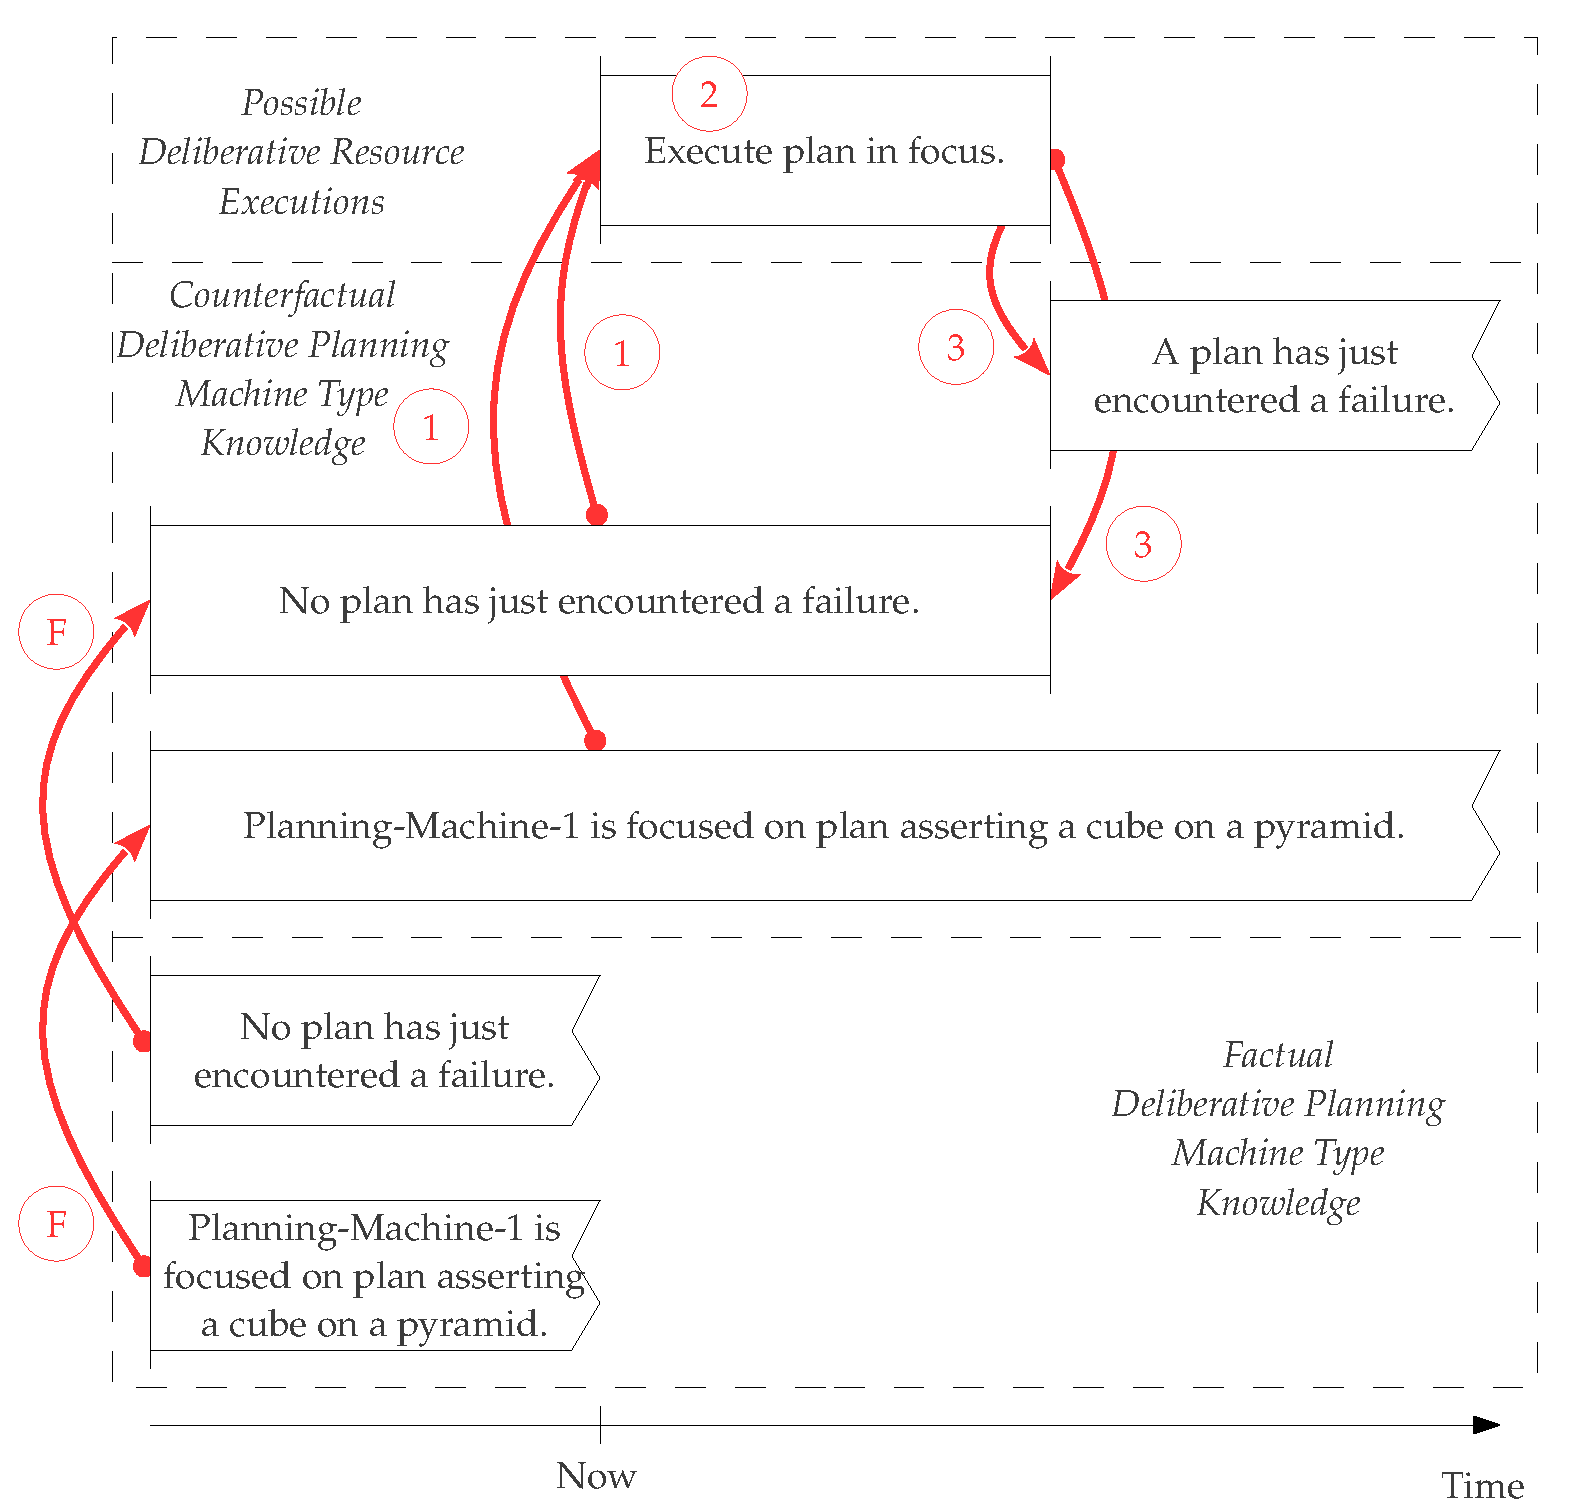
\includegraphics[width=12cm]{gfx/inference_of_deliberative_planning_machine_knowledge}
\caption[Inference of counterfactual deliberative planning machine
  type knowledge from factual deliberative planning machine type
  knowledge.]{Inference of counterfactual deliberative planning
  machine type knowledge from factual deliberative planning machine
  type knowledge.  Rectangular boxes represent events over time.  Some
  events have a jagged right edge to indicate that this event has no
  ending time.  Curved arrows represent different dependency
  relationships: (F) factual, (1) precondition, (2) potential resource
  execution, and (3) hypothetical change.  Preconditions, potential
  resource activations, and hypothetical changes form the three
  possibly unsupported parts of a dependency.  Factual dependencies
  cannot lose support because they are derived directly from factual
  events.}
\label{figure:inference_of_deliberative_planning_machine_knowledge}
\end{figure}


\section{Propagating Loss of Hypotheses to Counterfactual Inferences}

Plan knowledge that the AI has been told can inform its hypothesis
spaces for the potential changes that resource executions will cause,
allowing the AI to imagine both successful and unsuccessful
accomplishment of the goal condition of ``A block is sitting on a
block'' with different hypothetical supports.  When the AI executes
the resource, it refines these hypothesis spaces that predict these
changes given the factual preconditions and effects of the actual
resource execution.  The refinement of hypothesis spaces has the
potential to eliminate the hypotheses that have supported previous
counterfactual inferences.  In order to correct counterfactual
inferences when hypotheses are removed from hypothesis spaces, every
individual hypothesis in each resource execution transframe change
hypothesis space has a list of \emph{removal callbacks} that are
called if the hypothesis is ever removed from the hypothesis space.
So, when the hypothesis space is refined in light of new factual
evidence, dependencies that are supported by these hypotheses are
notified that they have become \emph{invalidated}.  When a dependency
has become invalidated, it has a chance to reconfigure its
hypothetical support, so that it can still predict the same
hypothetical change, and thus, still support the counterfactual
knowledge that depends upon it.  Here are the basic steps of the
grounded hypothesis refinement process that corrects and removes
unsupported counterfactual knowledge in light of new evidence and
refined hypothesis spaces:
\begin{enumerate}
\item When a resource execution transframe change hypothesis space is
  refined, removing hypotheses, registered callbacks for each of these
  hypotheses are called, invalidating the dependencies that are
  supported by these hypotheses.
\item Invalidated dependencies check to see if the resource execution
  transframe change hypothesis space still contains hypotheses that
  will support the change given the preconditions for the possible
  resource execution.
\item If the invalidated dependency can find new hypothetical support
  for the resource execution transframe change, it marks itself as
  valid and no counterfactual events are modified as the dependency
  has found new supporting hypotheses.
\item If the invalidated dependency cannot find new hypothetical
  support for the resource execution transframe change, it becomes
  unsupported and marks dependent counterfactual knowledge to be
  unsupported and removed from the counterfactual knowledge base.
\item If a counterfactual event loses the support of a dependency and
  is removed from the counterfactual knowledge base, those
  dependencies that are supported by these counterfactual events as
  preconditions are invalidated, causing the propagation of the
  refined hypothesis spaces to correct further counterfactual event knowledge.
\end{enumerate}

In this way, as hypothesis spaces are refined and hypotheses are
eliminated due to new factual evidence, the effects on the
counterfactual knowledge is minimized by first invalidating the
dependencies, allowing them to rearrange their supports where
possible, before dependencies give up and declare themselves as
unsupported to their dependent counterfactual events.

\section{Losing and Searching for New Hypothetical Support}

When the AI first imagines that executing its plan will result in ``A
cube is sitting on a pyramid,'' this counterfactual event is
associated with the newly created dependency shown in
{\mbox{\autoref{table:physical_dependency}}}.
\begin{table}[h]
\centering
\begin{tabular}{c}
  A Supported Dependency for Counterfactual \\
  Physical Type Knowledge Event \\
  ``A cube is sitting on a pyramid.'' \\
  \begin{tabular}{|p{3cm}|p{6cm}|}
    \hline
    \emph{possible resource execution:} & Drop and wait for block to fall. \\
    \hline
    \emph{preconditions:}               & \\
    \hline
    \emph{add hypotheses:}              & \emph{True} \\
    \hline
  \end{tabular}
\end{tabular}
\caption[A dependency for a counterfactual physical type knowledge
  event given no factual evidence.]{A dependency for a counterfactual
  physical type knowledge event given no factual evidence.  Notice
  that since this knowledge has ``been told'' to the AI without any
  experience executing this action, the hypothesis space has not been
  refined and the most general hypothesis, which predicts \emph{True}
  in all preconditions, is the only supporting hypothesis for this
  counterfactual event.}
\label{table:physical_dependency}
\end{table}
When the AI actually executes the ``Drop and wait for block to fall
resource'', the hypothesis space for the addition of ``A cube is
sitting on a pyramid'' is refined by removing those hypotheses that
are no longer consistent with the factual event knowledge.  The
hypothesis space reflects that in the specific preconditions of the
execution, the change did not occur.  However, the AI is not sure
about other possible preconditions.  In this case, the most general
hypothesis, which is \emph{True} in all preconditions, has been
removed from the hypothesis space.  This causes the dependency shown
in {\mbox{\autoref{table:physical_dependency}}} to become invalidated.
The dependency then attempts to find new hypothetical support for its
predicted change.  In this case, the dependency is not able to
reconfigure its support in order to mark itself as once again valid,
so the dependency becomes unsupported and removes the unsupported
counterfactual event that depends upon it.  The unsupported dependency
due to the loss of the most general hypothetical support is shown in
{\mbox{\autoref{table:physical_reconfigured_dependency}}}.
\begin{table}[h]
\centering
\begin{tabular}{c}
  An Unsupported Dependency for Counterfactual \\
  Physical Type Knowledge Event \\
  ``A cube is sitting on a pyramid.'' \\
  \begin{tabular}{|p{3cm}|p{6cm}|}
    \hline
    \emph{possible resource execution:} & Drop and wait for block to fall. \\
    \hline
    \emph{preconditions:}               & $A$: Gripper-1 is holding a block. \\
                                        & $B$: Gripper-1 is above a cube. \\
    \hline
    \emph{add hypotheses:}              & ${\neg}A \wedge B$ \\
                                        & $A \wedge {\neg}B$ \\
                                        & ${\neg}A \wedge {\neg}B$ \\
    \hline
  \end{tabular}
\end{tabular}
\caption[An unsupported dependency for a counterfactual physical type
  knowledge event after losing its original hypothetical support and
  attempting to reconfigure new support.]{An unsupported dependency
  for a counterfactual event after losing its original hypothetical
  support due to experience executing the reactive resource.  Note
  that this dependency has found a number of hypotheses that would
  provide support under different preconditions.}
\label{table:physical_reconfigured_dependency}
\end{table}

Initially the reflective layer of the AI has not been told any plans
that assert conditions of the deliberative planning machine type
knowledge.  This means that when the reflective layer imagines
executing the plan in focus, it does not predict a failure will occur.
However, when the AI has executed the plan to stack the cube on the
pyramid, this actually does result in a factual failure.  The AI
reflectively responds to the failure by imagining executing a new plan
for deliberative action.  The reflective layer infers the
counterfactual deliberative planning machine type knowledge shown in
{\mbox{\autoref{figure:inference_of_deliberative_planning_machine_knowledge}}}.
During this imaginative inference process, the reflective layer
creates the counterfactual event, ``A plan has just encountered a
failure'', which has the newly created dependency shown in
{\mbox{\autoref{table:deliberative_dependency}}}.
\begin{table}[h]
\centering
\begin{tabular}{c}
  A Supported Dependency for Counterfactual \\
  Deliberative Planning Machine Type Knowledge Event \\
  ``A plan has just encountered a failure.'' \\
  \begin{tabular}{|p{3cm}|p{6cm}|}
    \hline
    \emph{possible resource execution:} & Execute plan in focus. \\
    \hline
    \emph{preconditions:}               & $A$: No plan has just encountered a failure. \\
                                        & $B$: Planning-Machine-1 is focused on plan asserting a cube on a pyramid. \\
    \hline
    \emph{add hypotheses:}              & $A \wedge B$ \\
    \hline
  \end{tabular}
\end{tabular}
\caption[A dependency for a counterfactual deliberative planning
  machine type knowledge event given no factual evidence.]{A
  dependency for a counterfactual deliberative planning machine type
  knowledge event given the factual evidence of previously executing
  this deliberative resource once in the given deliberative planning
  machine type knowledge preconditions.}
\label{table:deliberative_dependency}
\end{table}
With the AI's new experience, it imagines executing another plan,
which asserts ``A pyramid is sitting on a cube.''  The execution of
the first plan is avoided due to the prediction of failure in the
reflective imaginative inference of counterfactual failure for this
plan.  When the new plan is selected, it finally succeeds in
accomplishing the physical goal condition: ``A block is sitting on a
block,'' demonstrating the abstract reflective imagination of plan
execution, in this case, helps to accomplish the primary physical goal
at hand.


\mymargins
\chapter{Virtual Machine and Programming Language}
\label{chapter:virtual_machine_and_programming_language}

The SALS AI is a cognitive architecture that is constructed on a
virtual machine and low-level Lisp-like programming language that
implicitly supports the tracing of results and behavior of the system
to the data and through the procedures that produced those results and
that behavior \cite[]{morgan:2009}.  Good traces make a system
accountable and help to enable the analysis of success and failure,
and thus enhancing the ability of the system to learn from mistakes.
The SALS virtual machine and low-level Lisp-like programming language
collectively form the substrate that executes the entire SALS
cognitive architecture.  In this chapter, I will focus on the details
of the low-level Lisp-like programming language that enable learning
from failure.  In
{\mbox{\autoref{chapter:learning_asynchronously_from_experience}}}, I
described the details of how an asynchronous learning algorithm can
learn from these failures so that these failures can be avoided in
future natural language plan executions through learning refined
causal models of the hypothetical imagined effects of natural language
plans.  In this chapter, I will describe the details of the low-level
Lisp-like language that enable these types of asynchronous learning
algorithms.

The SALS virtual machine provides for general parallelism and
concurrency, while supporting the automatic collection of audit trails
for all processes, including the processes that analyze audit trails.
The native support of a low-level Lisp-like language in the SALS
architecture allows, as in machine language, a program to be data that
can be easily manipulated by a program, making it easier for a user or
an automatic procedure to read, edit, and write programs as they are
debugged.  Large concurrent and parallel systems are often difficult
to build and debug because of the complex causal interactions between
all of the different processes.  For this reason, every parallel task
in SALS has an associated ``cause'' object.  If any task creates a new
parallel task, then a new cause object is created for the child task
with a parent cause object reference.  Cause objects represent
meta-information about a task, such as in what way a compiled
procedure should be executed, which can be used for causally
organizing the effects of groups of parallel tasks, controlling and
monitoring the occurrence of any type of event through any of the
procedural abstraction barriers of the SALS virtual machine.

\section{Virtual Machine}

The SALS virtual machine is designed to take advantage of the next
generation of multithreaded and multicore CPUs, so that new reflective
algorithms will more easily be designed to exhibit ``strong'' scaling
properties \cite[]{sodan:2010}.  In order to allow the development of
these new types of algorithms, the SALS virtual machine includes an
explicit representation, called a ``virtual processor'' object, that
represents each hyperthread in each core of each CPU in the target
hardware platform.  Each of the SALS virtual processors is used in
order to organize the scheduling of SALS ``fiber'' objects, which are
the bytecode threads that execute in the SALS virtual machine.  In
this way, each SALS fiber can be assigned to a specific hyperthread in
the target hardware platform.  In order to prevent local cache misses
for on-chip caches, the SALS virtual machine has a separate memory
pool allocated for each of the SALS virtual processors.  So, for CPUs
that has 4 cores and 2 hyperthreads per core, 8 memory pools are
allocated when the SALS virtual machine is created.  Also, a major
bottleneck in systems with large numbers of processors and cores are
mutual exclusion or ``mutex'' locks that protect shared resources.
The SALS virtual machine avoids all mutexes in the memory layer by
using these separate dedicated memory pools for each hyperthread in
each CPU core for memory allocation and concurrent garbage collection.
Mutexes are provided in the SALS architecture but low-level memory
allocation and collection can operate at full-speed without any mutex
locks for low-level memory operations.
{\mbox{\autoref{figure:cpu_core_hyperthread_distances}}} shows an
example of how SALS allocates virtual processors for a hardware
configuration with two processors, each having four cores and each
core having two hyperthreads.  Each hyperthread is organized into a
binary tree structure that is used in order to calculate distances
between hardware hyperthreads.  This binary tree distance metric is
used to dynamically distribute fiber loads across hyperthreaded CPU
cores in order to attempt to utilize as much on-chip CPU cache as
possible.
\begin{figure}
\centering
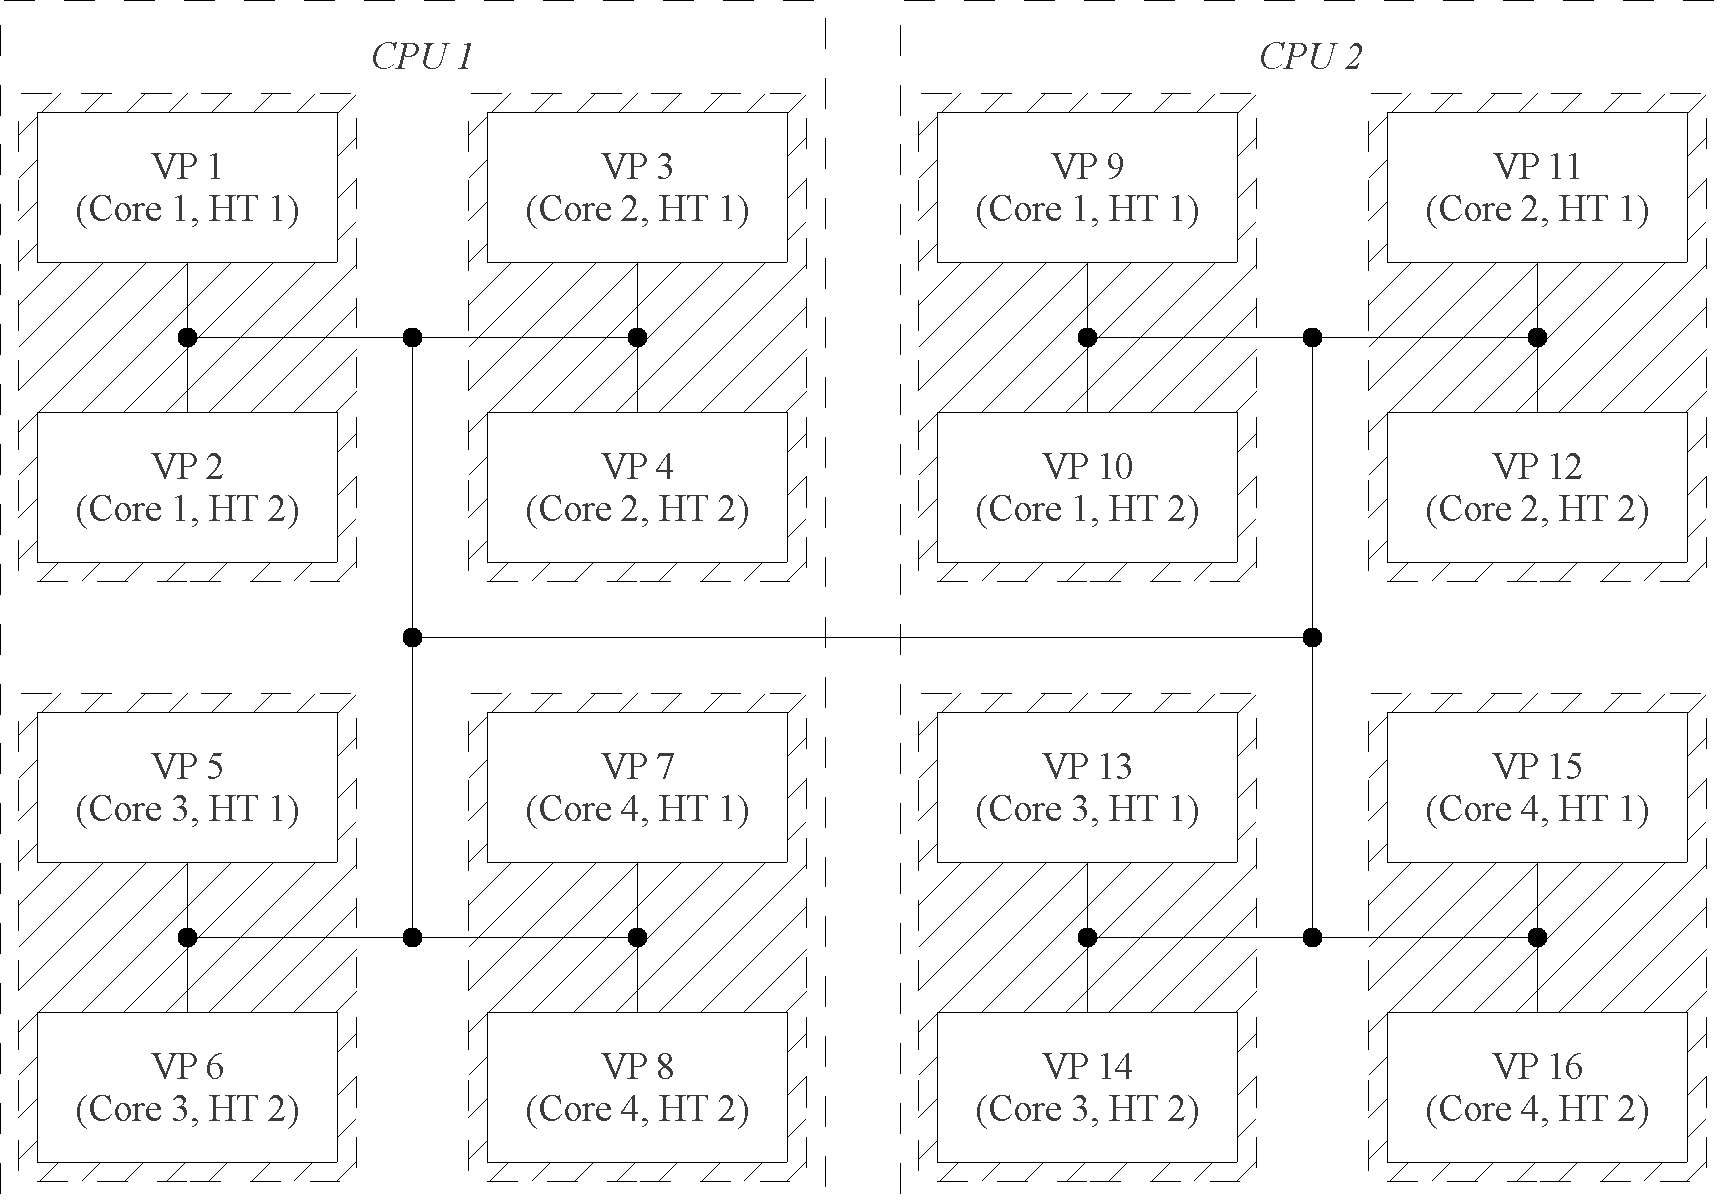
\includegraphics[width=12cm]{gfx/cpu_core_hyperthread_distances}
\caption[An example of how SALS allocates virtual processors for a
  hardware configuration with two multithreaded multicore
  processors.]{An example of how SALS allocates virtual processors
  (VP) for a hardware configuration with two multithreaded multicore
  processors, each having four cores and each core having two
  hyperthreads (HT).  Each hyperthread is organized into a binary tree
  structure that is used in order to calculate distances between
  hardware hyperthreads.  This binary tree distance metric is used to
  dynamically distribute fiber loads across hyperthreaded CPU cores in
  order to attempt to utilize as much on-chip CPU cache as possible.}
\label{figure:cpu_core_hyperthread_distances}
\end{figure}

The SALS virtual machine has been tested with a maximum of 32
processors and 128 gigabytes of RAM on the Nautilus supercomputer at
the National Institute for Computational Sciences.  However, most of
the examples presented in this dissertation have been executed on a
personal computer with only 4 CPU cores and 2 hyperthreads per core.
The SALS virtual machine has a tricolor garbage collection algorithm
that takes advantage of parallelizing work in concurrent processors.
Memory pointers in the SALS memory system are 64-bit integers that
have space reserved for three hierarchical memory tiers: (1)
``computer identity,'' (2) ``pool index,'' (3) and ``block address.''
{\mbox{\autoref{table:sals_memory_pointer}}} shows the bit allocation
within the 64-bit SALS memory pointer.
\begin{table}
\centering
\begin{tabular}{|l|l|l|}
\hline
\emph{bit range} &\emph{\# of values} &\emph{memory tier name} \\
\hline
~1 -- 17 &$131,072$         &computer identity \\ % 17
\hline
18 -- 27 &$1,024$           &pool index        \\ % 10
\hline
28 -- 64 &$137,438,953,472$ &block address     \\ % 37
\hline
\end{tabular}
\caption[Bit allocation within the SALS memory pointer.]{Bit
  allocation within the SALS memory pointer.}
\label{table:sals_memory_pointer}
\end{table}
The computer identity is zero if the memory pointer is referencing
memory on the local computer.  The computer identity is an integer
greater than zero if the memory is on another computer that has
connected to the SALS memory system through a low-level peer-to-peer
socket connection.  The ability of the SALS architecture to connect to
other running SALS architectures allows it to potentially scale to
take advantage of the hardware on multiple networked computers to
solve one large shared-memory problem.  The pool index is an integer
reference into an array of memory pools on the given computer.  On any
given computer, one memory pool is allocated for each hyperthread in
each CPU core on each CPU.  The block address is an integer that is a
block index into the given memory pool.  A block size of one byte has
been used for the examples presented in this dissertation but larger
block sizes have been tested and can be used if more memory must be
addressed.

\section{Package Manager}

The SALS programming language allows compiling and running computer
programs that consist of many thousands of lines of code.  For
example, the examples presented in this dissertation depend on loading
154 packages, which are composed of over 30,000 lines of code that are
written in the SALS low-level Lisp-like programming language.  The
SALS programming language includes a package manager in order to
organize dependencies within this codebase.  In addition to a
low-level Lisp-like codebase of packages, the SALS virtual machine has
the ability to load packages that contain optimized routines that are
composed of compiled machine code.  Machine code extensions to the
SALS virtual machine are written in the C programming language.  The C
codebase that compiles to this machine code totals over 150,000 lines
of C code.  The following is a declaration of a package definition in
the SALS low-level Lisp-like language that helps to organize these
different types of dependencies within the SALS codebase:
\begin{samepage}
\begin{Verbatim}
  [defpackage semantic_knowledge_base
    :packages          [equals_hash
                        forgetful_event_stream
                        semantic_realm
                        semantic_causal_event
                        semantic_relationship_key
                        semantic_frame
                        semantic_object
                        semantic_event]
    :sources           ['semantic_knowledge_base-core.sals']
    :dynamic_libraries ['libf2e_semantic_knowledge_base.so']]
\end{Verbatim}
\end{samepage}
The ``defpackage'' expression in the SALS programming language means
``define package.''  The first argument to the defpackage expression
is the name of the package to be defined, ``semantic knowledge base''
in this case.  The remaining arguments to the defpackage expression
are optional and three such arguments are shown in this example: (1)
``packages,'' (2) ``sources,'' and (3) ``dynamic libraries.''  The
``packages'' optional argument specifies a list of other packages that
must be loaded before this package is loaded.  The ``sources''
optional argument specifies a list of SALS low-level Lisp-like
programming language files that are to be loaded when this package is
loaded.  The ``dynamic libraries'' optional argument specifies a list
of files that contain machine code extensions that should be loaded
into the SALS virtual machine when this package is loaded.

Every package and machine code extension to the SALS virtual machine
and programming language performs ``causal reflective tracing'' on
each concurrently executing process.  The following sections describe
examples of different uses of the causal reflective tracing features
that have been implemented throughout the SALS virtual machine and its
extensions.  At the end of this chapter I will describe one high-level
package in the SALS programming language that performs the conjunctive
hypothesis space version space rule-learning algorithm, which is key
to the asynchronous experiential learning presented in
{\mbox{\autoref{chapter:learning_asynchronously_from_experience}}}.

\section{Causal Reflective Tracing}

Parallel tasks in the virtual machine are called ``fibers'' in order
to distinguish them from the ``threads'' in the underlying operating
system kernel.  The parallel fibers create, mutate, and read from
memory as they execute sequences of compiled bytecodes.  At any point
between bytecode executions, the memory system is static and can be
saved or loaded from non-volatile memory, such as a harddisk.  The
current execution state of every fiber is represented in the global
environment.  To be fully reflective on all of the procedural effects
of any given fiber, I introduce a technique called ``causal reflective
tracing.''  Causal reflective tracing is a way of defining variables
that are specific to each fiber that can be used to control the
low-level memory access, mutation, and creation functions.  This
allows one fiber to subscribe to the procedural trace events of
another fiber without receiving procedural trace events of its own
execution, which would lead to an infinite regress, halting the
system.  Further, because the virtual machine is inherently a parallel
processing system, a given fiber will often start a number of child
fibers that handle part of the processing for the parent fiber.  When
a new fiber is created, the child fiber inherits the causal variable
bindings of its parent fiber, enabling the same procedural tracing
options for the child as well.  So, causal reflective tracing is one
of the basic tools for keeping track of which pieces of memory were
created, mutated, or read by which other fibers.  When evaluating the
theoretical time complexity of concurrent procedurally reflective
control algorithms, it should be noted that creating procedural trace
events for the execution of a given fiber slows the fiber down only by
a constant factor, not affecting the algorithm's ``big-O'' time
complexity on an ideal concurrent shared-memory system, of which the
virtual machine is an approximation.

While causal reflective tracing focuses the procedural event tracing
to memory interactions of specific groups of fibers, this still
results in millions of events to consider every real-time second of
execution.  In order to further focus on specific objects within the
memory system, specific pieces of memory can be created called
``semantic memory.''  Semantic memory objects are created, mutated,
and accessed in roughly the same way as all of the frame-based objects
in the memory system with a few extra reflective tracing features.
For example, semantic objects provide event streams that can be
subscribed to by a number of different parallel listeners in different
fibers.  Also semantic object pointers are bidirectional in order to
ease traversal by reflective pattern matching algorithms.

Because it becomes awkward to subscribe to each and every frame-based
object that may be interesting to the reflective focus, semantic
frames that are created by specific fibers can be added to collections
of semantic frames that are called ``semantic knowledge bases.''
Semantic knowledge bases are good for organizing entire layers or
subsets of reflective layers that contain different types of semantic
frame objects.  Semantic knowledge bases allow the same forgetful
event stream subscription services as semantic frames with the
additional capability of tracing the addition and removal of entire
semantic frames to and from the knowledge base.

While knowledge base reconstructions are extremely fast to reference,
$O(1)$, they require a duplication of the memory requirements of the
focus knowledge base for every different point in time that is
required.  In order to allow efficient access of the state of
knowledge bases at arbitrary points in the past, ``semantic event
knowledge bases'' are another type of representation that is
reflectively and asynchronously maintained in order to not slow down
the primary procedure under reflective focus.
{\mbox{\autoref{chapter:learning_asynchronously_from_experience}}}
describes how the SALS asynchronous learning algorithm uses the event
knowledge base object to calculate partial state transframes.  I will
briefly review the features of the event knowledge base as well as a
few details about how this object is initialized and used in the SALS
low-level Lisp-like programming language.  The semantic event
knowledge base stores a type of semantic frame called a ``semantic
event.''  A semantic event is a type of semantic frame object that
represents an interval in time, which may include partial knowledge if
the start or end times do not exist, making the interval potentially
open-ended.  Semantic event knowledge bases are reflectively traced
and the knowledge is always stored in two different representations,
the basic semantic event frames as well as a balanced interval tree
that always represents the current state of the semantic event
knowledge base.  The balanced interval tree allows accessing the state
of the focus knowledge base in $O(\log{(n)})$ time, where $n$ is the
number of events stored in the semantic event knowledge base.
Although the time complexity is not as efficient as the constant,
$O(1)$, access time of the reflectively reconstructed semantic
knowledge base, the semantic event interval tree knowledge base only
requires $O(n)$ memory complexity in order to allow access to the
structure of the knowledge base at any point in the past, where $n$ is
the number of semantic events.
{\mbox{\autoref{figure:semantic_event_knowledge_base}}} shows how to
create a new ``{\tt{semantic\_event\_knowledge\_base}}'' type object
in the SALS low-level Lisp-like interactive programming language.
\begin{figure}[h]
\centering
{\scriptsize
\begin{Verbatim}[frame=single]
 in-> [new semantic_event_knowledge_base nil [new semantic_realm]]
out-> [semantic_event_knowledge_base
        semantic_event_tree         [semantic_event_tree ...]
        semantic_frame_set          [set ...]
        trace_remove_semantic_frame []
        trace_callback_funks_frame  [frame ...]
        semantic_realm              [semantic_realm ...]
        trace_event_stream          [forgetful_event_stream ...]
        trace_add_semantic_frame    []
        ...]
\end{Verbatim}
}
\caption[How to create a new
  ``{\tt{semantic\_event\_knowledge\_base}}'' type object.]{How to
  create a new ``{\tt{semantic\_event\_knowledge\_base}}'' type
  object.  When ``{\tt{semantic\_event}}'' type objects are added,
  removed, or modified while they are in this type of knowledge base,
  the knowledge base updates an always-accurate event interval tree
  structure for all of the events for efficient, $O(\log{(n)})$,
  access to the events at any point in time.}
\label{figure:semantic_event_knowledge_base}
\end{figure}

By default, when there are no listeners to the procedural event
streams of a semantic frame-based object, no reflective events are
created, allowing the use of the object to run at full speed.  When a
listener subscribes to the procedural use of a specific semantic
memory object, events are added to ordered streams for the listening
subscribers.  In order to conserve memory resources, when multiple
parallel listeners are subscribed to a given event stream, only those
events that have not already been seen by all of the subscribers are
remembered.  Once all subscribers have processed an event, all events
before this event are forgotten.  This type of memory conserving event
stream is referred to as a ``forgetful event stream.''  In this way
semantic frames report the addition and removal of slot values to
reflective forgetful event stream subscribers.  Once a knowledge base
is created and we have an ``important event stream iterator,'' we can
define a concurrent reflective fiber that processes the events
reflectively, after the real-time execution of the processes that
modify this knowledge base.
{\mbox{\autoref{figure:reflective_fiber}}} shows an example of how a
reflective fiber can be created to process a
{\tt{forgetful\_event\_stream}} generated by a
{\tt{semantic\_knowledge\_base}}, which includes a traced
{\tt{semantic\_planner}}.
\begin{figure}[h]
\centering
{\scriptsize
\begin{Verbatim}[frame=single]
 in-> [let* [[realm          [new semantic_realm]]
             [knowledge_base [new semantic_event_knowledge_base
                                  nil realm]]
             [iterator       [get knowledge_base
                                  new-event_stream_iterator]]
             [planner        [new semantic_planner realm]]]

        'Start parallel reflective fiber.'
        [fiber [funk []
                 [while t
                   [let [[event [have iterator wait_for_current]]]
                     [print event]
                     [have iterator increment]]]]
               []]
        
        [set planner trace_add    t]
        [set planner trace_remove t]
        
        [have knowledge_base add_semantic_frame planner]
        
        [set planner imagine_time [new semantic_time [time]]]]
out-> []
\end{Verbatim}
}
\caption[A reflective fiber can be created to process an
  {\tt{forgetful\_event\_stream}}.]{A reflective fiber can be created
  to process a {\tt{forgetful\_event\_stream}} generated by a
  {\tt{semantic\_knowledge\_base}}, which includes a traced
  {\tt{semantic\_planner}}.  Note that this example runs at a constant
  factor slower than full speed because of the creation of mutation
  events for the {\tt{semantic\_planner}} object, but this factor has
  been kept relatively small, so this example completes almost
  immediately.  The reflective process runs slower because it must
  consider how to print these events to the terminal in a readable
  form.  {\mbox{\autoref{figure:remove_add_set_events}}} shows the
  last two events created by the last line of this example that
  mutates the {\tt{imagine\_time}} slot value for the planner.}
\label{figure:reflective_fiber}
\end{figure}

\begin{figure}[h]
\centering
{\scriptsize
\begin{Verbatim}[frame=single]
[semantic_frame_event
  time           [time
                   years        2012
                   months       8
                   days         31
                   ...]
  event_type     remove
  semantic_frame [semantic_planner
                   property phenomenal_name [...]
                   property planner_type    [[]]
                   property imagine_time    [[semantic_time ...]]
                   relation execute_plan    [[]]
                   relation imagine_plan    [[]]
                   relation focus_plan      [[]]
                   ...]
  key_type       property
  key            imagine_time
  value          []]
\end{Verbatim}
\begin{Verbatim}[frame=single]
[semantic_frame_event
  time           [time years 2012 months 8 days 31 hours 23 ...]
  event_type     add
  semantic_frame [semantic_planner
                   property phenomenal_name [...]
                   property planner_type    [...]
                   property imagine_time    [...]
                   relation execute_plan    [...]
                   ...]
  key_type       property
  key            imagine_time
  value          [semantic_time
                   value [time
                           years        2012
                           months       8
                           days         31
                           ...]]]
\end{Verbatim}
}
\caption[The last two events created by the last line of the example
  in {\mbox{\autoref{figure:reflective_fiber}}}.]{The last two events
  created by the last line of the example in
  {\mbox{\autoref{figure:reflective_fiber}}}:
  ``{\tt{[set~planner~imagine\_time~[new~semantic\_time~[time]]]}}''. This
  command mutates the {\tt{imagine\_time}} slot value for the planner.
  Notice that the first of the two events is a {\tt{remove}} type of
  event, while the second is an {\tt{add}} type event.  This event
  knowledge is used in the SALS AI to create reconstructions of entire
  knowledge bases of physical as well as deliberative object types,
  like planners.  Note that the first event removes the {\tt{[]}} slot
  value of the {\tt{imagine\_time}} {\tt{property}} of the
  {\tt{semantic\_planner}} object, while the second event adds the new
  value, thus completing the mutation.}
\label{figure:remove_add_set_events}
\end{figure}

While every parallel fiber is allocated a unique {\tt{cause}} object
that provides a representation of the reflective tracing features for
that fiber, sometimes it is useful to collect events from overlapping
sets or different hierarchies of many fiber objects.  A convenient
solution to causally organizing very dynamic sets of fibers is
provided by a ``cause group'' object.  Cause groups are added to cause
objects and inherited from parent to child when new causes are
created.  Because cause objects and cause group objects exist at the
locus of every memory creation and mutation event in the SALS virtual
machine, they provide a means of tracing any event that modifies any
part of the SALS virtual machine.
{\mbox{\autoref{figure:cause_group_statistics}}} shows an example of
causal reflective tracing that takes advantage of cause group objects
in order to gather run-time statistics of a fiber execution.
{\mbox{\autoref{figure:hierarchical_cause_group_statistics}}} shows
another example of using a hierarchy of multiple cause group objects
in order to causally scope the tracing of $30$ parallel fibers that
are hierarchically organized into $3$ cause groups that contain $10$
fibers each.
\begin{figure}[h]
\centering
{\scriptsize
\begin{Verbatim}[frame=single]
 in-> [globalize cause_group [new cause_group]]
out-> []

 in-> [with-new-cause
        [have [this-cause] add_cause_group cause_group]
        [partimes [i 10]
          [print i]]]
0
1
2
3
4
6
7

58
9
out-> []

 in-> cause_group
out-> [cause_group
        execution_nanoseconds 533248657
        bytes_allocated_count 2766181
        bytecode_count        19495
        bytes_freed_count     0]
\end{Verbatim}
}
\caption[Using a {\tt{cause\_group}} object to gather statistics from
  causally scoped executions.]{Using a {\tt{cause\_group}} object to
  gather statistics from causally scoped executions.  A new
  {\tt{cause\_group}} object is first created in the global
  environment.  The gathering of run-time statistics involves creating
  a new cause with the ``{\tt{with-new-cause}}'' operator, adding this
  cause to the {\tt{cause\_group}} object, and subsequently running an
  experiment.  This example creates ten parallel fibers that each
  print their numerical index from $0$ to $9$.  At the final output of
  the example, the global {\tt{cause\_group}} object is printed to the
  screen, showing processor execution time, total bytes allocated,
  total bytecodes executed, and also the number of bytes garbage
  collected during the experiment.}
\label{figure:cause_group_statistics}
\end{figure}
\begin{figure}[h]
\centering
{\scriptsize
\begin{Verbatim}[frame=single]
 in-> [globalize cause_group [new cause_group]]
out-> []

 in-> [let [[begin_time [time]]
            [frame      [new frame]]]
        [with-new-cause
          [have [this-cause] add_cause_group cause_group]
          [partimes [i 3]
            [let [[subcause_group [new cause_group]]]
              [have frame add i subcause_group]
              [with-new-cause
                [have [this-cause] add_cause_group subcause_group]
                [partimes [j 10]
                  [terminal_format standard-terminal j]]]]]]
        [have frame add `real-time [- [time] begin_time]]
        frame]
024031548162062794915695337878                      
out-> [frame
        0         [cause_group
                    execution_nanoseconds 3535418608
                    bytes_allocated_count 7715763
                    ...]
        2         [cause_group
                    execution_nanoseconds 3012761500
                    bytes_allocated_count 7590735
                    ...]
        1         [cause_group
                    execution_nanoseconds 3976116760
                    bytes_allocated_count 9598095
                    ...]
        real-time [relative_time
                    seconds      1
                    milliseconds 694
                    ...]]

 in-> cause_group
out-> [cause_group
        execution_nanoseconds 10730429054
        bytes_allocated_count 25622218
        bytecode_count        215649
        bytes_freed_count     0]
\end{Verbatim}
}
\caption[Gathering run-time statistics using parallel hierarchies of
  causal scopes.]{Gathering run-time statistics using parallel
  hierarchies of causal scopes.  Overall, $30$ parallel fibers are
  created, each prints a number from $0$ to $9$, and run-time
  statistics are gathered in two layers of causal scope hierarchy.
  The overall {\tt{cause\_group}} object is shown last, while three
  sub-{\tt{cause\_group}} objects are printed as the return value of
  the second expression.  Notice that the algorithm uses $10.7$
  seconds of processor time, while only using $1.7$ seconds of
  real-time.}
\label{figure:hierarchical_cause_group_statistics}
\end{figure}

Sometimes it is helpful to know which fiber or cause created a
specific piece of memory.  For this reason, every piece of memory in
the entire virtual machine includes a reference to its creation cause
as well as its creation fiber.
{\mbox{\autoref{figure:reflective_event_causal_tracing}}} shows how a
fiber can retrieve the creation cause of a semantic event object, it
is useful to know which fiber or cause is responsible for creating a
given semantic event object so that a reflective fiber can learn from
the separate effects of different causal scopes that make
modifications to semantic objects within a given knowledge base.  This
form of causal tracing is used in the SALS cognitive architecture to
detect when one resource interacts with another resource, for example,
by activating that resource or waiting for that resource to complete
execution.  An entire reflective knowledge base of current parallel
resource interactions is maintained by tracing the causes of resource
interactions in this way.
\begin{figure}[h]
\centering
{\scriptsize
\begin{Verbatim}[frame=single]
 in-> [let* [[realm          [new semantic_realm]]
             [knowledge_base [new semantic_event_knowledge_base
                                  nil realm]]
             [iterator       [get knowledge_base
                                  new-event_stream_iterator]]
             [planner        [new semantic_planner realm]]]

        'Start parallel reflective fiber.'
        [fiber [funk []
                 [while t
                   [let* [[event       [have iterator
                                             wait_for_current]]
                          [event-cause [get event cause]]]
                     [if [eq `my-test [have event-cause lookup
                                            `cause-name]]
                         [print `event-in-causal-focus]
                       [print `event-out-of-causal-focus]]
                     [have iterator increment]]]]
               []]
        
        [set planner trace_add    t]
        [set planner trace_remove t]
        
        [have knowledge_base add_semantic_frame planner]
        
        [with-new-cause
          [cause-define cause-name `my-test]
          [set planner imagine_time [new semantic_time [time]]]]]
out-> []
event-out-of-causal-focus
event-out-of-causal-focus
event-out-of-causal-focus
event-out-of-causal-focus
event-out-of-causal-focus
event-out-of-causal-focus
event-out-of-causal-focus
event-out-of-causal-focus
event-in-causal-focus
event-in-causal-focus
\end{Verbatim}
}
\caption[Causally scoped reflective event tracing.]{Causally scoped
  reflective event tracing.  Since every piece of memory in the
  virtual machine has a reference to its {\tt{cause}} object, causally
  focusing the reflective tracing example shown in
  {\mbox{\autoref{figure:reflective_fiber}}} is simply a matter of
  accessing the creation cause of each event, using the expression,
  {\tt{[get event cause]}}.}
\label{figure:reflective_event_causal_tracing}
\end{figure}

\section{Conjunctive Hypothesis Version Space Rule-Learning}

The SALS architecture includes a ``version space''
\cite[]{mitchell:1997} hypothesis rule-learning algorithm.  A use of
this hypothesis version space rule-learning algorithm was described in
{\mbox{\autoref{chapter:learning_asynchronously_from_experience}}} as
part of a larger asynchronous learning algorithm that learns to
predict the partial state ``transframe'' \cite[]{minsky:1975} effects
of resource executions given the partial state preconditions of the
execution.  The hypothesis version space rule-learning algorithm
included in the SALS architecture predicts one binary output feature
given a number of binary input features.  The benefit of the version
space rule-learning algorithm is that it provides a relatively compact
representation of an entire conjunctive hypothesis space by only
representing the most general and most specific boundaries in the
overall lattice of potential hypotheses.  The included rule-learning
algorithm is incremental, meaning that it refines its space of
hypotheses as new examples of training data become known.  The SALS AI
hypothesis version space learning algorithm also includes ``removal
callbacks'' for most general and most specific hypotheses, so that if
these hypotheses are no longer supported given new training data,
these hooks allow tracing dependencies for correcting hypothetically
supported counterfactual knowledge in the counterfactual knowledge
base of each planning layer of the SALS AI.
{\mbox{\autoref{figure:concept_version_space}}} shows how to create a
{\tt{concept\_version\_space}} object that can be trained.
{\mbox{\autoref{figure:concept_version_space_training}}} shows an
example of training the {\tt{concept\_version\_space}} object, given
training examples.
{\mbox{\autoref{figure:concept_version_space_hypothetical_support}}}
shows how hypothesis removal callbacks can be used to monitor the loss
of support for a specific example, attempting to find new support
whenever the previous hypothetical support is lost.
\begin{figure}[h]
\centering
{\scriptsize
\begin{Verbatim}[frame=single]
 in-> [new concept_version_space]

out-> [concept_version_space
        specific_hypotheses [[concept_version_space_hypothesis]]
        general_hypotheses  [[concept_version_space_hypothesis]]
        variable_name_set   [set elements []]]
\end{Verbatim}
}
\caption[Creating a new {\tt{concept\_version\_space}} conjunctive
  hypothesis learning algorithm.]{Creating a new
  {\tt{concept\_version\_space}} conjunctive hypothesis learning
  algorithm.  This object keeps a list of the most specific hypotheses
  that support positive output predictions as well as the most general
  hypotheses that support negative output predictions.  Also, there is
  a set of variable names, or frame slot names, that the algorithm has
  seen previously.}
\label{figure:concept_version_space}
\end{figure}
\begin{figure}[h]
\centering
{\scriptsize
\begin{Verbatim}[frame=single]
 in-> [let [[concept [new concept_version_space]]]
   
        'Add a positive training example to the concept.'
        [let [[example [new concept_version_space_example t]]]
          [have example add_variable_value `color `blue]
          [have example add_variable_value `shape `cube]
          [have concept train_on_example example]]

        [terminal_format standard-terminal
                         '\ntrain-1: ' concept]
        
        'Add a negative training example to the concept.'
        [let [[example [new concept_version_space_example nil]]]
          [have example add_variable_value `color `blue]
          [have example add_variable_value `shape `pyramid]
          [have concept train_on_example example]]
        
        concept]
train-1: [concept_version_space
           specific_hypotheses [[concept_version_space_hypothesis
                                  shape cube
                                  color blue]]
           general_hypotheses  [[concept_version_space_hypothesis
                                  shape ?
                                  color ?]]]
out-> [concept_version_space
        specific_hypotheses [[concept_version_space_hypothesis
                               shape cube
                               color blue]]
        general_hypotheses  [[concept_version_space_hypothesis
                               shape cube
                               color ?]]]
\end{Verbatim}
}
\caption[Training a {\tt{concept\_version\_space}} conjunctive
  hypothesis learning algorithm.]{Training a
  {\tt{concept\_version\_space}} conjunctive hypothesis learning
  algorithm.  A new {\tt{concept\_version\_space}} is created.  Two
  {\tt{concept\_version\_space\_example}}s are created, one positive
  and one negative.  The concept is printed after learning from the
  positive example.  The final concept is returned after being trained
  on both examples.}
\label{figure:concept_version_space_training}
\end{figure}
\begin{figure}[h]
\centering
{\scriptsize
\begin{Verbatim}[frame=single]
 in-> [let [[concept [new concept_version_space]]]
        [print 'Training on positive example.']
        [let [[example [new concept_version_space_example t]]]
          [have example add_variable_value `color `blue]
          [have example add_variable_value `shape `cube]
          [have concept train_on_example example]]
        [print 'Adding removal callbacks to hypotheses.']
        [let [[example [new concept_version_space_example t]]]
          [have example add_variable_value `color `green]
          [have example add_variable_value `shape `cube]
          [label find_new_support []
            [mapc [funk [hypothesis]
                    [terminal_format standard-terminal
                                     '\nNew supporting '
                                     'hypothesis: ' hypothesis]
                    [have hypothesis add_removal_callback
                                     [funk []
                                       [print 'Lost support.']
                                       [find_new_support]]
                                     []]]
                  [get concept supporting_hypotheses example]]]
          [find_new_support]]
        [print 'Training on negative example.']
        [let [[example [new concept_version_space_example nil]]]
          [have example add_variable_value `color `blue]
          [have example add_variable_value `shape `pyramid]
          [have concept train_on_example example]]
        [print 'Done.']
        nil]
'Training on positive example.'
'Adding removal callbacks to hypotheses.'
New supporting hypothesis: [concept_version_space_hypothesis
                             shape ?
                             color ?]
'Training on negative example.'
'Lost support.'
New supporting hypothesis: [concept_version_space_hypothesis
                             shape cube
                             color ?]
'Done.'
out-> []
\end{Verbatim}
}
\caption[Hypothesis removal callbacks used to monitor the loss of
  support for a specific example, attempting to find new support
  whenever the previous hypothetical support is lost.]{Hypothesis
  removal callbacks monitor the loss of support for a specific
  example, attempting to find new support whenever the previous
  hypothetical support is lost.  In this case, a positive example of a
  {\tt{green}} {\tt{cube}} is attempting to maintain hypothetical
  support in the concept's hypothesis space.}
\label{figure:concept_version_space_hypothetical_support}
\end{figure}




\mymargins
\cleardoublepage\part{Related Work}\label{part:related_work}
\mymargins
%************************************************
\chapter{Related Models}
\label{chapter:related_models}
%************************************************

\section{The Emotion Machine v1.0}

One previously developed cognitive architecture that implements
commonsense reasoning, based on Minsky's Emotion Machine theory of
mind \cite[]{minsky:2006}, is a metareasoning system for correcting
faulty plans, called EM-ONE (Emotion Machine, v1)
\cite[]{singh:2005b}. EM-ONE is written in Lisp, using a Prolog
extension as a logical resolution tool. EM-ONE is a layered
architecture consisting of reactive, deliberative, and reflective
layers. Mental critics are represented as commonsense narratives that
result in queries to a collection of different Prolog knowledge
bases. The commonsense narratives are given to the system in a Lisp
format that is compiled into the knowledge bases as collections of
horn clauses. These knowledge bases consist of collections of
domain-specific horn clauses that are divided into physical, social,
and mental domains of reasoning. On top of this Prolog logical
substrate, the Lisp program is organized into layers as a
critic-selector model of mind. The narrative plans that are generated
by the deliberative layer are executed by a lower-layer, called the
reactive layer. Part of the reactive layer of the algorithm is written
in C and runs PID control loops in a simulated social two-wheeled
inverted pendulum type robot. EM-ONE demonstrates how a system can use
commonsense narratives in order to reason by analogy in order to
generate plans. Also, EM-ONE demonstrates a learning process that is a
carefully crafted collection of reflective critics that recognize
types of social failures to infer the goals of other AIs.  Because of
the complexity of the rigid-body physics in the world, sometimes even
the most carefully constructed plans fail. EM-ONE has a layer of
reflective critics that debug deliberative narratives as they are
being interpreted by using a collection of commonsense narrative
debugging critics.  Using narratives about social situations, EM-ONE
infers the goals of the other AIs in the world given partial knowledge
of their visible physical actions. When mistakes are made in this
inference process, the failure is recognized reflectively, after the
fact. Specific types of debugging responses are implemented for
different forms of critical failures. EM-ONE is a step toward a large
and complex commonsense reasoning AI with multiple layers of
metareasoning that inspect, control, and debug mental representations.

In my AI, I have focused on implementing a form of learning where
resource executions are of constant time complexity, $O(1)$, so that
there are no search algorithms operating ``behind the scenes'', such
as those in any system based on Prolog with its implicit logical
resolution of declarative program statements.  The substrate presented
in this thesis is developed with the intention of building a stable
platform for larger cognitive architectures in the same vein as
EM-ONE.  For this reason, the substrate presented in this thesis is
distributed as an extensible open-source program that can be easily
downloaded, modified and used by others.  The rigid body physics
simulation implemented in EM-ONE has been extended in capability with
our kitchen cooking simulator, IsisWorld \cite[]{smith:2010}, which
allows experimenting with multiple social AIs in a rigid-body physical
kitchen that can work together to learn how to perform cooperative
cooking tasks.

\section{Interior Grounding}

\cite{minsky:2005} describes an evolutionary reflective model of mind
called \emph{interior grounding}.  Interior grounding states that each
layer of reflective thinking could be genetically predestined to each
have different and specific types of useful ways of thinking.  Minsky
rejects the \emph{physical grounding hypothesis}, which stipulates
that thoughts must necessarily develop from the lowest layer first and
only subsequently to the higher layers of thinking.

Because my AI is modelled after Minsky's Emotion Machine cognitive
architecture, activities in the mind can create and manipulate
symbolic arrangements without these symbols necessarily referring to
the physical layer of activity.  My model considers factual grounding
in both the perception of physical knowledge as well as the perception
of internal mental states, such as the deliberative planning machine
knowledge.

In terms of the Emotion Machine cognitive architecture, each
reflective layer of my model can be considered to have a unique
built-in reactive layer, which makes room for these genetic
dispositions that Minsky describes as the basis for interior
grounding.  My AI demonstrates interior grounding by having sets of
factual knowledge as the control domain for both the deliberative as
well as the reflective planning machines, so factual grounding of
hypothetical counterfactual inferences in my AI need not begin by
reasoning about physical activity, growing from lower layers to higher
layers, but may instead begin by reasoning about the factual events in
the deliberative planning machine knowledge bases.

\section{Metareasoning}

\cite{cox_and_raja:2008,cox:2010} present a reflective model of mind
called \emph{metareasoning}.  My AI demonstrates metareasoning in the
reflective layer, which controls the deliberative planning machine.
The metareasoning described by Cox and Raja begins with a ``ground
level'', which corresponds to the physical knowledge base in my AI,
then describe how a second level, the ``object level'', is a control
loop that receives perceptions from the ground level, processes these,
and sends actionable commands back to the ground level.  The
metacognitive object level corresponds with the deliberative layer and
the deliberative planning machine knowledge base in my AI.  They then
proceed to a third level, which completes two cascaded control loops:
one controlling the ground level with another controlling the object
level.  This third level is called the ``meta-level''.  Cox and Raja's
meta-level corresponds to the reflective layer and reflective planning
machine knowledge base in my AI.
\begin{figure}[bth]
\begin{align*}
\text{Cox and Raja's Ground Level } &{\approx} \text{ Reactive Layers} \\
\text{Cox and Raja's Object Level } &{\approx} \text{ Deliberative Layer} \\
\text{Cox and Raja's Meta-Level }   &{\approx} \text{ Reflective Layer}
\end{align*}
\caption{The lower levels of Cox and Raja's metareasoning model mapped
  to the Emotion Machine cognitive architecture presented in this
  thesis.}
\label{figure:metareasoning_as_reflective_order_notation}
\end{figure}
\autoref{figure:metareasoning_as_reflective_order_notation} shows how
Cox and Raja's levels map to the Emotion Machine cognitive
architecture presented in this thesis.  Here they explain what happens
when the object level fails in either the creation or execution of a
plan:
\begin{quote}
When reasoning fails at some task, it may involve the explanation of
the causal contributions of failure and the diagnosis of the
object-level reasoning process.
\end{quote}
Cox and Raja explain how debugging causal models of the reasoning
process itself is a form of meta-level reasoning, or reflective layer
of thinking.  My model has a separate distinct class of resource
activation hypotheses for the separate layers of deliberative and
reflective thinking, so learning physical causal models is a distinct
activity from reflectively learning deliberative thinking causal
models.  The implementation demonstrates how two distinct layers of
hypothetical inference models allow not only learning to act but also
learning to think about acting.



\mymargins
\cleardoublepage\part{Evaluation, Future, and Concluding Remarks}\label{part:evaluation_future_and_concluding_remarks}
\mymargins
%************************************************
\chapter{Evaluation}
\label{chapter:evaluation}
%************************************************

This dissertation consists of four contributions that work together to
form the SALS AI.  From the low-level virtual machine and Lisp-like
programming language to the reflective and super-reflective layers of
the Emotion Machine cognitive architecture, it is difficult to
evaluate all aspects of the SALS AI by a single simple metric.
Therefore, this chapter presents a number of different metrics that
are used to measure all of the four contributions presented in this
dissertation:
\begin{packed_enumerate}
\item{\emph{Emotion Machine Cognitive Architecture}: The primary
  contribution of this thesis is a recursive implementation of a
  reflective planning layer that controls a deliberative planning
  process.  Because of the recursive nature of the implementation, a
  super-reflective layer is also used to control and learn about the
  reflective planning process.  The benefit of adding each additional
  reflective layer is that more can be learned from each deliberative
  failure by adding each additional reflective layer, but there is a
  computational trade-off in that each additional reflective layer
  also increases the computational complexity of the overall
  architecture.  This chapter evaluates the Emotion Machine cognitive
  architectural component of the SALS AI by asking the following
  question: What is the increase in computational complexity
  introduced by adding additional reflective planning layers to the
  basic deliberative planning process?  The answer to this question is
  not at first obvious because of the exponentially larger state-space
  confronted by each higher planning layer.  The result is that each
  additional layer adds a roughly linear increase in computational
  complexity to the overall architecture.  This chapter discusses how
  the increased computational complexity of each additional reflective
  planning layer is kept from becoming exponential in the SALS AI.
  This chapter also discusses how using concurrent hardware in order
  to separately simulate each additional reflective layer has the
  potential to reduce the overall time-complexity of the architecture
  to sub-linear per additional layer.}
\item{\emph{Learning from Being Told Natural Language Plans}: The
  ability of each planning layer in the SALS AI to interpret and
  imagine the effects of ambiguous natural language plans relies on a
  search through possible interpretations of each natural language
  phrase in any given plan.  This search would quickly become
  intractable if it were not controlled by a number of different types
  of low-level programmatic constraints.  Only those natural language
  plan interpretations that make programmatic sense according to these
  constraints are further considered for imagination or execution.  In
  practice, each low-level constraint helps to reduce the overall
  search complexity by varying amounts depending on the domain of
  control, whether the natural language plan is describing a control
  process for the physical, deliberative, or reflective knowledge
  domains.  This chapter shows empirical results that compare the size
  of the overall natural language plan interpretation search with and
  without each of these constraints for the control of each knowledge
  domain in the SALS AI.  This chapter also discusses the trade-offs
  between introducing language specific constraints, such as
  English-only semantics or syntax, versus purely programmatic
  constraints that keep the SALS natural planning language as it is
  currently applicable to all natural human languages.}
\item{\emph{Learning Asynchronously from Experience}: The ability of
  each planning layer in the SALS AI to asynchronously abstract the
  partial state events in its control knowledge domain as well as
  asynchronously learn rule-based causal models of resource
  activations of the layer below introduces two potentially
  problematic scaling factors for the computational complexity of the
  overall SALS AI.  Firstly, the number of partial states in arbitrary
  knowledge domains could in the worst case introduce a factorial
  growth with the size of the knowledge domain and the size of the
  partial states being abstracted.  As factorial growth would be an
  intractable scaling factor for the computational complexity, this
  chapter shows empirical evidence for the actual scaling factors for
  abstracting partial states from each of the control knowledge
  domains, including the physical, deliberative, and reflective
  knowledge domains.  The causal hypothesis rule-learning algorithm
  could potentially even have a worse scaling factor that is a
  multiplier on the number of partial states abstracted in the first
  asynchronous stage in the SALS AI's learning from experience.  This
  chapter will also present empirical evidence of the actual scaling
  factor introduced by the conjunctive rule-learning algorithm
  employed in learning causal models of resource activations in the
  SALS AI for each planning layer, including the deliberative,
  reflective, and super-reflective layers.}
\item{\emph{Virtual Machine and Programming Language}: The SALS AI is
  constructed on a low-level virtual machine and Lisp-like programming
  language that takes advantage of multithreaded and multicore CPUs.
  The SALS virtual machine executes concurrent bytecode processes that
  are called ``fibers,'' which are an abstraction of the POSIX threads
  provided by the underlying operating system.  In order to minimize
  hyperthread-specific cache-miss effects for each concurrently
  executing fiber, a separate memory pool is allocated for each
  hardware hyperthread in each CPU core in the underlying hardware
  platform.  The SALS virtual machine performs dynamic load balancing
  in order to take advantage of as many CPU cores as possible while
  executing multiple fibers.  Also, the SALS virtual machine includes
  a concurrent tricolor garbage collection algorithm that has been
  optimized to be used over multiple memory pools.  In a perfect
  symmetric multiprocessing (SMP) system, executing $N$ fibers on $N$
  processors should have a constant time-complexity, but modern
  multithreaded and multicore CPUs have shared caches between
  hyperthreads and cores, which makes systems based on these CPUs less
  than ideal SMPs.  Furthermore, mutual exclusion (mutex) locks
  required for garbage collection slow down garbage collection across
  multiple memory pools by a factor depending on the number of
  cross-references between pools.  This chapter empirically evaluates
  how the SALS virtual machine performs at minimizing these cache-miss
  and locking effects on an Intel Core i7 CPU, which has 4 cores, each
  with 2 hyperthreads, while executing various numbers of concurrent
  fibers.}
\end{packed_enumerate}

\section{Computational Complexity of Reflective Layers}

The SALS AI consists of 100 parallel heterogeneous resources,
organized into 29 agencies, which comprise the 5 layers.  The causal
procedurally reflective tracing features of the SALS virtual machine
that have been described in
{\mbox{\autoref{chapter:virtual_machine_and_programming_language}}}
allow for the run-time evaluation of each separate causally scoped
component of the SALS AI.  In the evaluation of the complexity of each
additional reflective layer, the following execution events are
measured:
\begin{packed_enumerate}
\item{Memory Allocation in Bytes}
\item{Garbage Collection in Bytes}
\item{Bytecode Execution Count}
\item{Semantic Frame Slot Mutations}
\item{Plan Interpretation Nodes Considered}
\item{Analogical Plan Matches Considered}
\end{packed_enumerate}
Each planning layer in the SALS AI can be used to specify very similar
types of goals.  For example, consider the following three different
pieces of knowledge:
\begin{packed_enumerate}
\item{``A pyramid is on a cube.''}
\item{``A deliberative planner has the positive goal for a pyramid to
  be on a cube.''}
\item{``A reflective planner has the positive goal for a deliberative
  planner to have the positive goal for a pyramid to be on a cube.''}
\end{packed_enumerate}
This is the feared, worst-case scenario that the analogical language
interpretation process in each subsequently higher reflective layer of
reasoning becomes an exponentially more difficult problem.  In
general, however, this is not true because reflective reasoning does
not and in practice often does not involve directly interpreting these
types of exponentially more difficult natural language interpretation
problems.  This is because reflective natural language plans are very
rarely directly about specific states of knowledge in the physical
knowledge base as in these examples.  Usually, reflective knowledge is
about much simpler partial states of the deliberative planning machine
that do not involve any physical knowledge at all.  For example,
consider the following pieces of knowledge:
\begin{packed_enumerate}
\item{``A deliberative planner is focused on a plan that has failed.''}
\item{``A reflective planner is focused on a plan that has failed.''}
\end{packed_enumerate}

{\mbox{\autoref{table:plan_interpretation_computational_complexity_of_layers}}}
shows measures of computational complexity for each planning layer in
SALS AI as it goes through the learning scenario presented in the
introduction to this dissertation.
\begin{table}
\centering
\begin{tabular}{|l|l|l|l|l|}
\hline
                 &Alloc &GC &BC &Mutate \\
\hline
Deliberative     &      &   &   &       \\
\hline
Reflective       &      &   &   &       \\
\hline
Super Reflective &      &   &   &       \\
\hline
\end{tabular}
\caption{Computational complexity of plan interpretation for each
  planning layer.}
\label{table:plan_interpretation_computational_complexity_of_layers}
\end{table}
In order to measure the increase in computational complexity
introduced by adding additional reflective planning layers to the
basic deliberative planning process,   While more can be learned from
each deliberative failure by adding additional reflective planning
layers, each additional reflective layer also increases the
computational complexity of the overall architecture.  First, let us
consider the computational complexity of the deliberative planning
layer.

The answer to this question is not at first obvious because of the
exponentially larger state-space confronted by each higher planning
layer.

The result is that each additional layer adds a roughly linear
increase in computational complexity to the overall architecture.

This chapter discusses how the increased computational complexity of
each additional reflective planning layer is kept from becoming
exponential in the SALS AI.

This chapter also discusses how using concurrent hardware in order to
separately simulate each additional reflective layer has the potential
to reduce the overall time-complexity of the architecture to
sub-linear per additional layer.

\section{Computational Scaling of Natural Language Interpretation Constraints}

\section{Computational Scaling of Partial State Abstraction and Rule-Learning}

Given that each planning layer in the SALS AI is based on perceiving
and acting based on the existence or non-existence of partial states
in the knowledge base that is being controlled by the planning layer,
the state-space of the control domain that is perceived and reacted to
by a planning layer is directly related to the number of partial
states that can be abstracted from this control domain.  For example,
if we consider that the knowledge base that is being controlled by a
given planning layer is represented as a graph, which is not exactly
correct but will suit our purposes here, the set of partial states
that can be abstracted from this control domain includes a subset of
all possible subgraphs of this graph representation.  In order to
avoid an intractable number of partial states being automatically
abstracted from a given knowledge base, the types of partial states
that the SALS AI abstracts are limited to the ``relationship'' and
``property'' types of partial states described in
{\mbox{\autoref{chapter:learning_asynchronously_from_experience}}}.
These simple types of partial states limit the complexity



%\begin{equation}
%({2^n}-1)\left(\frac{n(n-1)}{2}\right)^{\ell}
%\end{equation}


\section{Computational Scaling of Concurrent Processing Hardware}


%% \section{old stuff}

%% \section{Boot-up and Perceive Experiment}

%% As an initial evaluation of the run-time performance of the AI, I have
%% run an experiment that simply initializes the AI and lets it perceive
%% the world over time.  The physical world does not change during this
%% experiment and the AI is not given any goals to accomplish, so this
%% experiment is a control that shows the baseline memory usage and
%% run-time performance of the cognitive architecture in its ``idling''
%% mode.  This experiment shows that the mind takes $10$ minutes to
%% initialize.  After initializing, the AI learns from its initial
%% perception and continues to attempt to detect changes in its raw
%% visual input over the next $50$ minutes.  Over the $50$ minutes of
%% continuous perception, the mind uses a highly fluctuating amount of
%% memory that stays, on average, relatively constant.  The mind is not
%% static in this experiment.  The mind contains resources that allocate
%% an average of $1.8$ megabytes per second in the built-in reactive
%% layer process of detecting visual changes in the next state from the
%% physical simulation, so that these changes may be propagated to the
%% physical knowledge of the learned reactive layer in a stream of
%% events.  Over $6$ gigabytes of memory is allocated over the entire
%% $60$ minutes of the experiment.  The mind uses an average memory
%% footprint of about $26$ megabytes over the course of the experiment.
%% The bytecode execution rate stabilizes at about $12$ thousand
%% bytecodes per second.  The concurrent processing capabilities of the
%% architecture can handle bursts of $50$ thousand bytecodes per second,
%% but this experiment simply shows that the execution rate of the
%% architecture does not slow down over time.  The entire cognitive
%% architecture exhibits stable handling of continuous processing for
%% experiments lasting over an hour, handling the allocation and garbage
%% collection of many gigabytes of memory in the process.
%% {\mbox{\autoref{figure:data/bootup_evaluation/mind_plot-Gripper-1}}}
%% shows a plotted overview of the run-time performance of the AI during
%% the boot-up and perceive experiment.  \autoref{table:bootup} on page
%% \pageref{table:bootup} shows more detailed plots for the run-time
%% behavior of each individual layer and agency within the AI.
%% %\experimentAIdatafigures[60]{bootup_evaluation}{an experiment that
%% %  boots up the AI, allowing it to continue to perceive the physical
%% %  world over time without stimulating it to achieve any goals.  This
%% %  experiment shows that the AI learns from its initial perceptions,
%% %  and when these do not change, it has nothing to learn and memory
%% %  usage is stable.}

%% \section{Deliberative Learning Experiment without Reflection}

%% The second run-time experiment that was performed with the cognitive
%% architecture does not include the reflective learning component that
%% learns hypothetical models for how the deliberative resources modify
%% the planning machine type knowledge base.  The AI is initialized,
%% which takes the same $10$ minutes as in the initial experiment.  The
%% AI is then told to execute a deliberative plan, which causes it to
%% execute a plan that attempts to stack a cube on top of a pyramid.  In
%% learning the effects of reactive resource executions on the physical
%% type knowledge bases the deliberative AI allocates $5.3$ megabytes per
%% second, while the memory footprint only grows at a rate of $90$
%% thousand bytes per second due to the learning that occurs over the
%% $60$ minutes that it takes to fail to accomplish this goal.  The AI
%% does not respond to the failure because the reflective layers are not
%% active.  The AI allocates an average of $1.2$ megabytes of memory per
%% second for the length of the experiment, which results in a total of
%% $5.4$ gigabytes over the course of the experiment.  The architecture
%% executes an average of $11$ thousand bytecodes per second over the
%% course of the experiment.  This shows that the architecture slows down
%% when more resources are active than simply the reactive perceptual
%% resources.  As deliberative learning resources become active, the
%% bytecode rate does not decrease much from the $12$ thousand bytecodes
%% per second in the control, but the overall memory allocation rate does
%% decrease by a factor of $66$\% from $1.8$ megabytes per second in the
%% control to $1.2$ megabytes per second with deliberative learning
%% enabled.
%% {\mbox{\autoref{figure:data/no_reflective_learning_evaluation/mind_plot-Gripper-1}}}
%% shows a plotted overview of the run-time performance of the AI during
%% the deliberative learning experiment with the reflective layer
%% disabled.  \autoref{table:no_reflective_learning} on page
%% \pageref{table:no_reflective_learning} shows plots of data for the
%% entire mind, each layer, as well as each agency within each layer for
%% this deliberative learning experiment.
%% %\experimentAIdatafigures[75]{no_reflective_learning_evaluation}{an
%% %  experiment with the reflective tracing of the deliberative process
%% %  disabled.  This experiment can be compared with run-time behavior of
%% %  the full AI cognitive architecture, which can learn from the failure
%% %  and initiate a second attempt at plan selection and execution.}

%% \section{Deliberative and Reflective Learning Experiment (The Full Architecture)}

%% The third run-time experiment that was performed with the cognitive
%% architecture includes both the deliberative as well as reflective
%% learning layers.  The deliberative layer learns hypothetical models of
%% the reactive resource execution effects on the physical type knowledge
%% base, while the reflective layer learns hypothetical models of the
%% deliberative resource execution effects on the deliberative planning
%% machine type knowledge base.  Although this experiment involves an
%% initial imaginative and plan selection processes in the reflective
%% layer, this experiment runs very similarly through the first $75$
%% minutes of otherwise mostly deliberative and reactive resource
%% executions.  Around minute $75$, the cognitive architecture responds
%% to the failure in the deliberative planning machine with the
%% reflective bug response, which begins another round of reflective
%% learning, imagination, and refined plan selection.  After a reflective
%% bug response, the goal is accomplished successfully around minute
%% $105$.  The experiment is allowed to run continuously after this point
%% for a total of $180$ minutes in order to show the performance of
%% baseline perceptual activity after going through the complete process
%% of deliberative and reflective learning.  Except for a blip at minute
%% $135$, which requires an extended garbage collection period, the AI is
%% otherwise stable after both layers have successfully demonstrated
%% learning.  With the addition of the reflective learning layer in the
%% final experiment the average bytecode execution rate has dropped
%% significantly, running at a factor $55$\% of the execution rate of the
%% architecture in the experiment demonstrating only deliberative
%% learning.  This experiment demonstrates the taxing demand of the extra
%% concurrent processes and memory allocation required with the
%% additional reflective learning algorithm.  However, slowing the
%% algorithm down by a factor of two with the addition of a reflective
%% layer of learning shows that the slow down is roughly linear with the
%% additional layer.  For example, in a naive approach to reflective
%% learning, an exponential increase in processing would be expected
%% because all resource executions and knowledge in the layers below
%% would be reflected upon and modelled by the reflective layer.  Because
%% the reflective learner implemented in this architecture only reflects
%% over the deliberative planning machine and not all of the processing
%% in the layers below, this architecture shows a linear slowdown with
%% the addition of reflective layers of learning.
%% {\mbox{\autoref{figure:data/reflective_learning_evaluation/mind_plot-Gripper-1}}}
%% shows a plotted overview of the run-time performance of the AI during
%% the reflective learning experiment.
%% \autoref{table:reflective_learning} on page
%% \pageref{table:reflective_learning} shows plots of data for the entire
%% mind, each layer, as well as each agency within each layer for this
%% reflective learning experiment, showing the run-time performance of
%% the full architecture.
%% %\experimentAIdatafigures[180]{reflective_learning_evaluation}{an
%% %  experiment testing the full AI cognitive architecture, including the
%% %  reflective tracing of the deliberative planning process, imagining
%% %  the potential failures of the deliberative planning machine as well
%% %  as the physical effects of physical actions.}

%% \section{No Theoretical Slowdown of Original Algorithm}

%% In order to assume that there is no theoretical slowdown of the
%% original planning algorithm when reflective learning is applied, it
%% must be assumed that the reflective implementation is an ideal
%% concurrent shared memory architecture.  In practice, the underlying
%% Funk virtual operating system slows down when more concurrent and
%% parallel tasks are executing.  This is beside the theoretical point,
%% but the following table shows a real-time test of the actual slowdown
%% experienced by the Funk operating system as different numbers of
%% parallel tasks are executed to perform a simple numerical processing
%% task.  The test was done on a dual Pentium processor computer, each
%% with ``core duo'' technology with each core implementing
%% ``hyper-threading'', which ends up appearing as eight processors to
%% the Linux operating system underlying the Funk virtual operating
%% system:

%% \vspace{5mm}
%% \begin{tabular}{ll}
%% Tasks & Real-Time (s) \\
%% 1 & 29\\
%% 2 & 36\\
%% 3 & 46\\
%% 4 & 44\\
%% 5 & 68\\
%% 6 & 67\\
%% 7 & 73\\
%% 8 & 110\\
%% \end{tabular}
%% \vspace{5mm}

%% As each additional concurrent resource in the cognitive architecture
%% begins execution, this table shows the approximate slowdown that the
%% Funk virtual machine experiences on this specific dual processor
%% hardware.


%\mymargins
%\cleardoublepage\part{Future}\label{part:future}
\mymargins
%*****************************************
\chapter{Future}\label{chapter:future}
%*****************************************

\label{section:model_6_future_research}

I began discussing strong parallels between my model and Minsky's
six-layered reflective theory of mind, called The Emotion Machine or
Model-6, in \autoref{backreference:self_reflective_self_conscious}.
Now I will continue a description of the top two layers of Minsky's
model in the theoretical terms of my model.

\section{Objective Reflection}

The ability to abstract object and subject distinctions within the
mind is key to how I see the creation of selves.  The primary object
abstractions would necessarily be based on physical activities that
lead toward or against physical goals.  An object has subjective
perspectives and extents in Space.  Further, every subjective
perspective would usefully have a set of causal hypotheses that lead
to and away from the object's more central subjective perspectives.
Objects, therefore, become collections of subjective perspectives that
can be easily traversed given the included causal models.  The extent
of an object in Space gives a useful Spatial arrangement for causal
hypotheses that help to create controllable boundaries around similar
perceptual and goal activities.

For example, this makes sense from a survivability standpoint.  The
most important and the first subject and object distinctions are those
that help accomplish or avoid physical goals.  In creating the
distinction that allows the mind to see the physical body as subjected
to the objects of a physical world, the mind has created one of the
first subjective perspectives, the physical body.

\section{Circular Objects}

Causal hypotheses are used in order to predict the future occurrence
of symbolic perceptions and goals.  Through reflective thinking, plans
are constructed from causal hypotheses consistent with the past,
elaborating the necessities in the past and the results in the future.
Analogies between consistent plans can be abstracted into models of
objects.  For example, a plan that begins and ends with the same
symbolic perception could be considered an example of a ``circular''
object; thus, an analogical plan abstraction would represent a type of
object, that has multiple sides to perceive depending on the subject's
position in the plan.  Circular objects may be an important type of
object to analogically recognize because a circular object allows one
to perform actions while being able to get back to a known perceptual
symbol.  If one is in a known circular object, then one is not lost in
the sense that one can always follow the circle in order to get back
to any perceptual symbol contained within the circular plan object.
My implementation includes tools for performing analogical
abstractions and constructions of plans, but this machinery is not key
to my thesis of explaining causal reflective learning to accomplish
goals.  I include this section in the dissertation to eliminate a
potential confusion that would conflate the concept of symbol with
that of object.  Symbols are the most primitive elements available to
thinking, while objects are more complicated in that they are composed
of analogical consistencies between plans that are themselves composed
of many symbols.  Objects have multiple subjective perspectives.
Objects are artificial creations of a mind, based on artificial static
symbols representing the ongoing activity in Duration.

\section{Body and World}

An intelligent mind builds models that predict the occurrence of
perceptual symbols.  Analogical thinking is used to abstract objects
and simultaneously the implied subjective perspectives on these
objects as they are manipulated.  The separation between the physical
body and the physical world is an objective form of thinking that is
fundamentally caused by goals that emphasize distinguishing bodily and
worldly goals in the causal structures of the physical perceptions.
For example, physical actions that change physical perceptions in
predictable ways are often bodily physical perceptions, i.e. moving
ones hand in front of ones face causes one to consistently see a hand.
Also, physical pain perceptions could be related to physical goals
that emphasize the artificial separation between the body and the
world.  Understanding the artificial separation of the body and the
world allows for an objective form of scientific study that places the
object of study in the world outside of the effects of the body.

\section{$m^\text{th}$-Stratum Objective Reflection}

Above this ability to model multiple interacting objects is the
ability to model objects as containing objects of the self-same type.
The ability to abstract all of the layers of a reflective mind into
one type of object or another can be used to recursively model one
object's model of another object.  Therefore, although my model does
not include objective reflection, I see this form of reflection as
along a new dimension that has, as its origin, all of the reflective
layers that I have so far described in my model.  I will refer to this
new dimension as ordered \emph{strata} of the \emph{objective
  dimension of reflective thinking}.

\begin{align}
\label{equation:objective_0_reflective_stratum}
\text{objective}^0\text{ reflective stratum } &{\approx} \bigcup_{n=0}^{\infty}{\text{reflective}^n\text{ layer}} \\
\label{equation:objective_m_reflective_stratum}
\text{objective}^m\text{ reflective stratum } &{\approx} \bigcup_{n=0}^{\infty}{\text{objective}^m\text{ reflective}^n\text{ layer}}
\end{align}

Prior to the first objective thinking stratum existing, it must have a
prior part of the mind upon which to objectively reflect.  I will
refer to all of the reflective layers I've described so far as the
zeroth-stratum of objective thinking, the ``$\text{objective}^0$''
stratum, since it contains no objective thinking at all.  Therefore,
the $m^\text{th}$-stratum of objective thinking in my model can be
described as ``$\text{objective}^m$'' reflective thinking.  Given this
notation, the self-reflective layer of Minsky's model would be the
first-stratum of objective thinking, or $\text{objective}^1$ reflection,
in my model.  Each $\text{objective}^m$ reflective stratum in my model
contains an infinite number of $\text{objective}^m\text{ reflective}^n$
layers.
Equations~\ref{equation:objective_0_reflective_stratum}~and~\ref{equation:objective_m_reflective_stratum},
roughly and non-mathematically show how each objective thinking
stratum is composed of an infinite number of reflective layers.
Again, this notation is \emph{not} set theoretic, and thus, set
theoretical mathematics do not apply.

\begin{figure}[bth]
  \begin{align*}
    \left.
    \begin{array}{l}
      \text{Minsky's Problem Domain }\\
      \text{Minsky's Built-in Reactive Layer }\\
      \text{Minsky's Learned Reactive Layer }\\
      \text{Minsky's Deliberative Layer }\\
      \text{Minsky's Reflective Layer }\\
    \end{array}
    \right\}                               &{\approx} \bigcup_{n=0}^{\infty}{\text{objective}^0\text{ reflective}^n\text{ layer}} \\
                                           &{\approx} \text{ objective}^0\text{ reflective stratum} \\
  \end{align*}
  \begin{align*}
    \text{Minsky's Self-Reflective Layer } &{\approx} \bigcup_{n=0}^{\infty}{\text{objective}^1\text{ reflective}^n\text{ layer}} \\
                                           &{\approx} \text{ objective}^1\text{ reflective stratum} \\
  \end{align*}
  \begin{align*}
    \text{Minsky's Self-Conscious Layer }  &{\approx} \bigcup_{n=0}^{\infty}{\text{objective}^2\text{ reflective}^n\text{ layer}} \\
                                           &{\approx} \text{ objective}^2\text{ reflective stratum}
  \end{align*}
\caption{The top layers of Model-6 roughly mapped to my
  $\text{objective}^m\text{ reflective}^n$ stratum notation.}
\label{figure:model_6_as_reflective_stratum_notation}
\end{figure}

Minsky's ``self-conscious'' layer would thereby roughly correspond
with my $\text{objective}^2$ reflective stratum.  Having two levels of
recursion in a objective thinking sense, leads to the ability to
represent what one object references in terms of what another object
references in terms of the original object.
\autoref{figure:model_6_as_reflective_stratum_notation} shows roughly
how the levels of Minsky's theory can be related to my stratum
notation.

\section{Imprimers}

\cite{minsky:2006} explains that terms like ``guilt'' and ``pride''
can refer to self-conscious ways of thinking.  Minsky hypothesizes
that there are powerful ways of thinking that result when someone whom
one respects, like a parent, values or devalues their goals.  This
type of relationship between object models is named an \emph{imprimer
  relationship} by Minsky.  In this relationship, the parent plays the
role of what Minsky has named an \emph{imprimer}, in reference to the
ability of ducklings to learn, relatively arbitrarily, to trust and
follow a parent-like figure.  Since I do not know of a another word
for an object in this sort of imprinting relationship, I will simply
use Minsky's term: imprimer.  He hypothesizes that imprimers, such as
parents and caregivers, play an important role in unquestioned
knowledge inheritance in children.  This type of thinking about what
someone else is thinking about their goals requires at least two
strata of objective reflection in my model.


%\mymargins
%\cleardoublepage\part{Conclusion}\label{part:conclusion}
\mymargins
%************************************************
\chapter{Conclusion}
\label{chapter:conclusion}
%************************************************

Building a model of general human intelligence is a massive
engineering effort that includes the shared expertise between all of
the disciplines of cognitive science, including: philosophy,
artificial intelligence, psychology, linguistics, anthropology, and
neuroscience.  While this dissertation is focused on building an AI
that scales to novel forms of metacognition that occur at higher
layers of reflective intelligence than have before been modeled, I
hope that the future of the SALS architecture enjoys contributions
from all of the diverse sub-disciplines of cognitive science.  The
SALS AI is meant to be a user-friendly platform for encoding many
examples of intelligence from each of these disciplines that are
usually researched separately.  While the current strengths and
weaknesses of the SALS AI have been discussed throughout this
dissertation, I hope that the following features of the SALS
architecture help toward this collaborative end:
\begin{packed_enumerate}
\item{Simple Syntax.}
\item{Natural Language Programming Interface.}
\item{Object-Oriented Frame-Based Representations.}
\item{Cognitive Architectural Primitives, such as Resources, Agencies,
  Planning Layers, and Reflectively Traced Knowledge Bases.}
\item{Causal Organization of Parallel Processes.}
\item{Concurrent Virtual Machine.}
\item{Included Machine Learning and Graph Algorithms.}
\item{Extension Package Manager.}
\item{On-Line Documentation \cite[]{morgan:2012}.}
\item{Open-Source Community.}
\end{packed_enumerate}
Given that the current five-layered version of the SALS AI is designed
to take advantage of multicore processors with local cache, as
computer hardware trends toward CPUs with more cores on each chip with
each core being simpler and with more on-chip cache storing memory
local to computations, the SALS virtual machine is well placed to
benefit from this coming wave of distributed multithreaded hardware
platforms.  This dissertation has described the four contributions of
this thesis:
\begin{samepage}
\begin{packed_enumerate}
\item Emotion Machine Cognitive Architecture ({\mbox{\autoref{chapter:emotion_machine_cognitive_architecture}}})
\item Learning from Being Told Natural Language Plans ({\mbox{\autoref{chapter:learning_from_being_told}}})
\item Learning Asynchronously from Experience ({\mbox{\autoref{chapter:learning_asynchronously_from_experience}}})
\item Virtual Machine and Programming Language ({\mbox{\autoref{chapter:virtual_machine_and_programming_language}}})
\end{packed_enumerate}
\end{samepage}
{\mbox{\autoref{chapter:related_models}}} has compared the SALS AI to
a number of related contemporary research disciplines, including:
computational metacognition, meta-planning and meta-plan recognition,
optimality in metacognition, and massively multithreaded programming.
{\mbox{\autoref{chapter:evaluation}}} evaluates the SALS AI by showing
the reflective architecture to scale at a tractable linear increase in
time-complexity for each additional layer, which implies an $N$
layered metacognitive architecture that allows not only planning and
learning about a problem domain but also any number of reflective
layers of planning and learning about the thinking processes
themselves.  A number of promising directions for future research with
the SALS AI have been described in {\mbox{\autoref{chapter:future}}}:
\begin{packed_enumerate}
\item{Self-reflective and self-consciously reflective thinking, the
  top two layers of the Emotion Machine theory of human commonsense
  thinking \cite[]{minsky:2006}, including self-models and social
  knowledge.}
\item{Extending reflective planning layers downward into the domain of
  plans-to-perceive \cite[]{pryor:1992,pryorcollins:1995,velez:2011},
  so that the SALS AI can learn plans for abstracting spatial
  relations between symbolic perceptions, such as the visual routines
  first implemented by \cite{ullman:1984}.}
\item{Plan and meta-plan recognition as a way to include current
  research on reflective story understanding architectures.}
\item{General partial state abstraction processes.}
\item{A propagation model of knowledge maintenance that traces
  knowledge provenance from refined hypotheses learned from experience
  to plan goal accomplishment and avoidance hypotheses.}
\item{General grammar definitions for the natural language programming
  language.}
\item{More efficient usage of multicore, hyperthreaded, and
  multiple-processor hardware platforms as well as completion of the
  distributed processing model that is partially implemented in the
  memory layer of the SALS virtual machine, which would allow
  peer-to-peer distributed processor support.}
\end{packed_enumerate}
For more information about downloading and getting started
experimenting with the freely distributed open source implementation
of the SALS AI, please see {\mbox{\autoref{appendix:the_code}}}.



%*******************************************************
% Backmatter
%*******************************************************
\appendix
\mymargins
\cleardoublepage\part{Appendix}
\mymargins
\chapter{The Code}\label{appendix:the_code}

\section{Open-Source Download}

All of the code that I developed for this PhD is free and openly
developed, can be downloaded from my webpage, and compiled by simply
typing "./configure; make".  See the on-line Funk2 website for
download instruction for Funk, \url{http://funk2.org/}, for downloads,
documentation, user community resources, and latest news.  Also, see
\url{http://em-two.net/} for research news on my Moral Compass
cognitive architecture that currently is distributed with Funk.

\section{README}

\lstset{basicstyle=\scriptsize}
\begin{lstlisting}
funk2: causally reflective programming language

  funk2 [-x <command>] [-p <portnum>] [<source.fu2>]

    <source.fu2>

        A user supplied filename of file from which to read and execute source
        code after booting and before exiting.

    -x <command>  [:default [repl]]

        A user supplied command to execute after booting and before exiting.

    -p <portnum>  [:default 22222 :try anything from 22222 to 23221]

        The localhost peer-command-server port number.  Each copy of funk2
        sharing a network interface must be able to allocate a unique
        peer-command-server port number.



TO PERFORM LOCAL BUILD:

  ./configure
  make


TO RUN LOCAL BUILD:

  ./funk2.sh    (from original compile directory)


TO PERFORM SYSTEM-WIDE INSTALLATION:

  ./configure
  make
  make install  (as root)


TO RUN SYSTEM-WIDE INSTALLATION:

  funk2         (from anywhere on system)



Homepage:

  http://funk2.org/



Git Access:

  http://git.neuromin.de/


Last Modified: 2010.10.25

Code Mass

--------------------------------------------------------------------------------

    Lines of Funk2 Code.....:   53249 total
    Words of Funk2 Code.....:  261289 total
    Characters of Funk2 Code: 2688091 total

    Lines of C Code.........:  144868 total
    Words of C Code.........:  564287 total
    Characters of C Code....: 7718554 total

    Total Lines of Code.....:   199564 total
    Total Words of Code.....:   830914 total
    Total Characters of Code: 10537116 total

--------------------------------------------------------------------------------

README Last Generated: Wed Aug 22 19:20:31 EDT 2012
\end{lstlisting}

\section{File Listing}

\lstset{basicstyle=\scriptsize}
\begin{lstlisting}
c/configurator.c
c/debugbreak.c
c/f2_ansi.c
c/f2_ansi.h
c/f2_apropos.c
c/f2_apropos.h
c/f2_archconfig.h
c/f2_array.c
c/f2_array.h
c/f2_atomic.h
c/f2_buffered_file.c
c/f2_buffered_file.h
c/f2_buffered_socket.c
c/f2_buffered_socket.h
c/f2_bug.c
c/f2_bug.h
c/f2_bytecodes.c
c/f2_bytecodes.h
c/f2_cause.c
c/f2_cause.h
c/f2_chunk.c
c/f2_chunk.h
c/f2_circular_buffer.c
c/f2_circular_buffer.h
c/f2_command_line.c
c/f2_command_line.h
c/f2_compile.c
c/f2_compile.h
c/f2_compile_x86.c
c/f2_compile_x86.h
c/f2_core_extension.c
c/f2_core_extension_funk.c
c/f2_core_extension_funk.h
c/f2_core_extension.h
c/f2_cpu.c
c/f2_cpu.h
c/f2_debug_macros.h
c/f2_defragmenter.c
c/f2_defragmenter.h
c/f2_dlfcn.c
c/f2_dlfcn.h
c/f2_dptr.c
c/f2_dptr.h
c/f2_dynamic_memory.c
c/f2_dynamic_memory.h
c/f2_f2ptr_set.c
c/f2_f2ptr_set.h
c/f2_fiber.c
c/f2_fiber.h
c/f2_fileio.c
c/f2_fileio.h
c/f2_frame_objects.c
c/f2_frame_objects.h
c/f2_funk2_node.c
c/f2_funk2_node.h
c/f2_funktional.c
c/f2_funktional.h
c/f2_garbage_collector_block_header.c
c/f2_garbage_collector_block_header.h
c/f2_garbage_collector.c
c/f2_garbage_collector.h
c/f2_garbage_collector_pool.c
c/f2_garbage_collector_pool.h
c/f2_globalenv.c
c/f2_globalenv.h
c/f2_global.h
c/f2_glwindow.c
c/f2_glwindow.h
c/f2_gmodule.c
c/f2_gmodule.h
c/f2_graph.c
c/f2_graph_cluster.c
c/f2_graph_cluster.h
c/f2_graph.h
c/f2_graph_match_error_correcting.c
c/f2_graph_match_error_correcting.h
c/f2_graphviz.c
c/f2_graphviz.h
c/f2_hash.c
c/f2_hash.h
c/f2_heap.c
c/f2_heap.h
c/f2_html.c
c/f2_html.h
c/f2_larva.c
c/f2_larva.h
c/f2_load.c
c/f2_load.h
c/f2_malloc.c
c/f2_malloc.h
c/f2_management_thread.c
c/f2_management_thread.h
c/f2_matlab.c
c/f2_matlab.h
c/f2_memblock.c
c/f2_memblock.h
c/f2_memory.c
c/f2_memory.h
c/f2_memorypool.c
c/f2_memorypool.h
c/f2_module_registration.c
c/f2_module_registration.h
c/f2_natural_language.c
c/f2_natural_language.h
c/f2_never_delete_list.c
c/f2_never_delete_list.h
c/f2_nil.c
c/f2_nil.h
c/f2_number.c
c/f2_number.h
c/f2_object.c
c/f2_object.h
c/f2_opengl.c
c/f2_opengl.h
c/f2_optimize.c
c/f2_optimize.h
c/f2_os.h
c/f2_package.c
c/f2_package.h
c/f2_package_handler.c
c/f2_package_handler.h
c/f2_packet.c
c/f2_packet.h
c/f2_partial_order.c
c/f2_partial_order.h
c/f2_peer_command_server.c
c/f2_peer_command_server.h
c/f2_primes.c
c/f2_primes.h
c/f2_primfunks.c
c/f2_primfunks__errno.c
c/f2_primfunks__errno.h
c/f2_primfunks__fcntl.c
c/f2_primfunks__fcntl.h
c/f2_primfunks.h
c/f2_primfunks__ioctl.c
c/f2_primfunks__ioctl.h
c/f2_primfunks__locale.c
c/f2_primfunks__locale.h
c/f2_primfunks__stdlib.c
c/f2_primfunks__stdlib.h
c/f2_primobject__boolean.c
c/f2_primobject__boolean.h
c/f2_primobject__char_pointer.c
c/f2_primobject__char_pointer.h
c/f2_primobject__circular_buffer.c
c/f2_primobject__circular_buffer.h
c/f2_primobject__doublelinklist.c
c/f2_primobject__doublelinklist.h
c/f2_primobject__dynamic_library.c
c/f2_primobject__dynamic_library.h
c/f2_primobject__environment.c
c/f2_primobject__environment.h
c/f2_primobject__fiber_trigger.c
c/f2_primobject__fiber_trigger.h
c/f2_primobject__file_handle.c
c/f2_primobject__file_handle.h
c/f2_primobject__frame.c
c/f2_primobject__frame.h
c/f2_primobject__hash.c
c/f2_primobject__hash.h
c/f2_primobject__largeinteger.c
c/f2_primobject__largeinteger.h
c/f2_primobject__list.c
c/f2_primobject__list.h
c/f2_primobject__matrix.c
c/f2_primobject__matrix.h
c/f2_primobject__object.c
c/f2_primobject__object.h
c/f2_primobject__object_type.c
c/f2_primobject__object_type.h
c/f2_primobject__ptypehash.c
c/f2_primobject__ptypehash.h
c/f2_primobject__redblacktree.c
c/f2_primobject__redblacktree.h
c/f2_primobjects.c
c/f2_primobject__set.c
c/f2_primobject__set.h
c/f2_primobjects.h
c/f2_primobject__stream.c
c/f2_primobject__stream.h
c/f2_primobject__tensor.c
c/f2_primobject__tensor.h
c/f2_primobject__traced_cmutex.c
c/f2_primobject__traced_cmutex.h
c/f2_primobject_type.c
c/f2_primobject_type.h
c/f2_primobject_type_handler.c
c/f2_primobject_type_handler.h
c/f2_print.c
c/f2_print.h
c/f2_processor.c
c/f2_processor.h
c/f2_processor_mutex.c
c/f2_processor_mutex.h
c/f2_processor_thread.c
c/f2_processor_thread.h
c/f2_processor_thread_handler.c
c/f2_processor_thread_handler.h
c/f2_protected_alloc_array.c
c/f2_protected_alloc_array.h
c/f2_ptype.c
c/f2_ptype.h
c/f2_ptypes.c
c/f2_ptypes.h
c/f2_ptypes_memory.h
c/f2_ptypes_object_slots.c
c/f2_ptypes_object_slots.h
c/f2_reader.c
c/f2_reader.h
c/f2_redblacktree.c
c/f2_redblacktree.h
c/f2_reflective_memory.c
c/f2_scheduler.c
c/f2_scheduler.h
c/f2_scheduler_thread_controller.c
c/f2_scheduler_thread_controller.h
c/f2_set.c
c/f2_set.h
c/f2_signal.c
c/f2_signal.h
c/f2_simple_repl.c
c/f2_simple_repl.h
c/f2_socket.c
c/f2_socket_client.c
c/f2_socket_client.h
c/f2_socket.h
c/f2_socket_server.c
c/f2_socket_server.h
c/f2_sort.c
c/f2_sort.h
c/f2_staticmemory.c
c/f2_staticmemory.h
c/f2_status.c
c/f2_status.h
c/f2_string.c
c/f2_string.h
c/f2_surrogate_parent.c
c/f2_surrogate_parent.h
c/f2_system_file_handler.c
c/f2_system_file_handler.h
c/f2_system_headers.h
c/f2_system_processor.c
c/f2_system_processor.h
c/f2_terminal_print.c
c/f2_terminal_print.h
c/f2_termios.c
c/f2_termios.h
c/f2_time.c
c/f2_time.h
c/f2_trace.c
c/f2_trace.h
c/f2_tricolor_set.c
c/f2_tricolor_set.h
c/f2_user_thread_controller.c
c/f2_user_thread_controller.h
c/f2_virtual_processor.c
c/f2_virtual_processor.h
c/f2_virtual_processor_handler.c
c/f2_virtual_processor_handler.h
c/f2_virtual_processor_thread.c
c/f2_virtual_processor_thread.h
c/f2_xmlrpc.c
c/f2_xmlrpc.h
c/f2_zlib.c
c/f2_zlib.h
c/funk2.c
c/funk2.h
c/funk2_main.c
c/test.c
extension/blocks_world/blocks_world.c
extension/blocks_world/blocks_world.h
extension/cairo/cairo.c
extension/cairo/cairo.h
extension/conceptnet/conceptnet.c
extension/conceptnet/conceptnet.h
extension/concept_version_space/concept_version_space.c
extension/concept_version_space/concept_version_space.h
extension/equals_hash/equals_hash.c
extension/equals_hash/equals_hash.h
extension/event_stream/event_stream.c
extension/event_stream/event_stream.h
extension/fibermon/fibermon.c
extension/forgetful_event_stream/forgetful_event_stream.c
extension/forgetful_event_stream/forgetful_event_stream.h
extension/forward_planner/forward_planner.c
extension/frame_ball/frame_ball.c
extension/graph_isomorphism/graph_isomorphism.c
extension/graph_isomorphism/graph_isomorphism.h
extension/gtk_extension/gtk_extension.c
extension/gtk_extension/gtk_extension.h
extension/image/image.c
extension/image/image.h
extension/image_sequence/image_sequence.c
extension/image_sequence/image_sequence.h
extension/interval_tree/interval_tree.c
extension/interval_tree/interval_tree.h
extension/keyboard/keyboard.c
extension/keyboard/keyboard.h
extension/lick/lick.c
extension/lick/lick.h
extension/meta_semantic_knowledge_base/meta_semantic_knowledge_base.c
extension/meta_semantic_knowledge_base/meta_semantic_knowledge_base.h
extension/movie/movie.c
extension/movie/movie.h
extension/propogator/propogator.c
extension/propogator/propogator.h
extension/semantic_action_event/semantic_action_event.c
extension/semantic_action_event/semantic_action_event.h
extension/semantic_action_knowledge_base/semantic_action_knowledge_base.c
extension/semantic_action_knowledge_base/semantic_action_knowledge_base.h
extension/semantic_action/semantic_action.c
extension/semantic_action/semantic_action.h
extension/semantic_agent/semantic_agent.c
extension/semantic_agent/semantic_agent.h
extension/semantic_category/semantic_category.c
extension/semantic_category/semantic_category.h
extension/semantic_causal_concept/semantic_causal_concept.c
extension/semantic_causal_concept/semantic_causal_concept.h
extension/semantic_causal_event/semantic_causal_event.c
extension/semantic_causal_event/semantic_causal_event.h
extension/semantic_causal_object/semantic_causal_object.c
extension/semantic_causal_object/semantic_causal_object.h
extension/semantic_containment_object/semantic_containment_object.c
extension/semantic_containment_object/semantic_containment_object.h
extension/semantic_counterfactual_transframe/semantic_counterfactual_transframe.c
extension/semantic_counterfactual_transframe/semantic_counterfactual_transframe.h
extension/semantic_directed_action_event/semantic_directed_action_event.c
extension/semantic_directed_action_event/semantic_directed_action_event.h
extension/semantic_event_knowledge_base/semantic_event_knowledge_base.c
extension/semantic_event_knowledge_base/semantic_event_knowledge_base.h
extension/semantic_event/semantic_event.c
extension/semantic_event/semantic_event.h
extension/semantic_event_sequence/semantic_event_sequence.c
extension/semantic_event_sequence/semantic_event_sequence.h
extension/semantic_event_transframe/semantic_event_transframe.c
extension/semantic_event_transframe/semantic_event_transframe.h
extension/semantic_event_tree/semantic_event_tree.c
extension/semantic_event_tree/semantic_event_tree.h
extension/semantic_expectation_failure/semantic_expectation_failure.c
extension/semantic_expectation_failure/semantic_expectation_failure.h
extension/semantic_frame/semantic_frame.c
extension/semantic_frame/semantic_frame.h
extension/semantic_goal_action_causal_hypothesis/semantic_goal_action_causal_hypothesis.c
extension/semantic_goal_action_causal_hypothesis/semantic_goal_action_causal_hypothesis.h
extension/semantic_goal_event/semantic_goal_event.c
extension/semantic_goal_event/semantic_goal_event.h
extension/semantic_goal/semantic_goal.c
extension/semantic_goal/semantic_goal.h
extension/semantic_knowledge_base/semantic_knowledge_base.c
extension/semantic_knowledge_base/semantic_knowledge_base.h
extension/semantic_know_of_existence_event/semantic_know_of_existence_event.c
extension/semantic_know_of_existence_event/semantic_know_of_existence_event.h
extension/semantic_know_of_relationship_event/semantic_know_of_relationship_event.c
extension/semantic_know_of_relationship_event/semantic_know_of_relationship_event.h
extension/semantic_object/semantic_object.c
extension/semantic_object/semantic_object.h
extension/semantic_object_type_event/semantic_object_type_event.c
extension/semantic_object_type_event/semantic_object_type_event.h
extension/semantic_ordered_object/semantic_ordered_object.c
extension/semantic_ordered_object/semantic_ordered_object.h
extension/semantic_packable_object/semantic_packable_object.c
extension/semantic_packable_object/semantic_packable_object.h
extension/semantic_planner/semantic_planner.c
extension/semantic_planner/semantic_planner.h
extension/semantic_plan_object/semantic_plan_object.c
extension/semantic_plan_object/semantic_plan_object.h
extension/semantic_plan_object_type_event/semantic_plan_object_type_event.c
extension/semantic_plan_object_type_event/semantic_plan_object_type_event.h
extension/semantic_plan_object_type_relation_event/semantic_plan_object_type_relation_event.c
extension/semantic_plan_object_type_relation_event/semantic_plan_object_type_relation_event.h
extension/semantic_plan_operator_activation/semantic_plan_operator_activation.c
extension/semantic_plan_operator_activation/semantic_plan_operator_activation.h
extension/semantic_plan_operator_parallel/semantic_plan_operator_parallel.c
extension/semantic_plan_operator_parallel/semantic_plan_operator_parallel.h
extension/semantic_plan_operator_sequence/semantic_plan_operator_sequence.c
extension/semantic_plan_operator_sequence/semantic_plan_operator_sequence.h
extension/semantic_plan_operator_suppression/semantic_plan_operator_suppression.c
extension/semantic_plan_operator_suppression/semantic_plan_operator_suppression.h
extension/semantic_proprioception/semantic_proprioception.c
extension/semantic_proprioception/semantic_proprioception.h
extension/semantic_proprioceptual_object/semantic_proprioceptual_object.c
extension/semantic_proprioceptual_object/semantic_proprioceptual_object.h
extension/semantic_proprioceptual_orientation/semantic_proprioceptual_orientation.c
extension/semantic_proprioceptual_orientation/semantic_proprioceptual_orientation.h
extension/semantic_proprioceptual_position/semantic_proprioceptual_position.c
extension/semantic_proprioceptual_position/semantic_proprioceptual_position.h
extension/semantic_realm/semantic_realm.c
extension/semantic_realm/semantic_realm.h
extension/semantic_reflective_object/semantic_reflective_object.c
extension/semantic_reflective_object/semantic_reflective_object.h
extension/semantic_reflective_object_type_event/semantic_reflective_object_type_event.c
extension/semantic_reflective_object_type_event/semantic_reflective_object_type_event.h
extension/semantic_reflective_object_type_property_event/semantic_reflective_object_type_property_event.c
extension/semantic_reflective_object_type_property_event/semantic_reflective_object_type_property_event.h
extension/semantic_reflective_object_type_relation_event/semantic_reflective_object_type_relation_event.c
extension/semantic_reflective_object_type_relation_event/semantic_reflective_object_type_relation_event.h
extension/semantic_relationship_key/semantic_relationship_key.c
extension/semantic_relationship_key/semantic_relationship_key.h
extension/semantic_resource_action_event/semantic_resource_action_event.c
extension/semantic_resource_action_event/semantic_resource_action_event.h
extension/semantic_resource_action_sequence/semantic_resource_action_sequence.c
extension/semantic_resource_action_sequence/semantic_resource_action_sequence.h
extension/semantic_resource_event_knowledge_base/semantic_resource_event_knowledge_base.c
extension/semantic_resource_event_knowledge_base/semantic_resource_event_knowledge_base.h
extension/semantic_resource/semantic_resource.c
extension/semantic_resource/semantic_resource.h
extension/semantic_self/semantic_self.c
extension/semantic_self/semantic_self.h
extension/semantic_situation_category/semantic_situation_category.c
extension/semantic_situation_category/semantic_situation_category.h
extension/semantic_situation/semantic_situation.c
extension/semantic_situation/semantic_situation.h
extension/semantic_situation_transition/semantic_situation_transition.c
extension/semantic_situation_transition/semantic_situation_transition.h
extension/semantic_somatosensation/semantic_somatosensation.c
extension/semantic_somatosensation/semantic_somatosensation.h
extension/semantic_somatosensory_object/semantic_somatosensory_object.c
extension/semantic_somatosensory_object/semantic_somatosensory_object.h
extension/semantic_temporal_object/semantic_temporal_object.c
extension/semantic_temporal_object/semantic_temporal_object.h
extension/semantic_time/semantic_time.c
extension/semantic_time/semantic_time.h
extension/semantic_visual_object/semantic_visual_object.c
extension/semantic_visual_object/semantic_visual_object.h
extension/timeline/timeline.c
extension/timeline/timeline.h
extension/transframe/transframe.c
extension/transframe/transframe.h
test/keyboard-test/ncurses-test.c
python/funk2module/c/funk2module.c
python/funk2module/c/funk2test.c
fu2/action.fu2
fu2/actor.fu2
fu2/actortest.fu2
fu2/assembler.fu2
fu2/bootstrap-apropos.fu2
fu2/bootstrap-array.fu2
fu2/bootstrap-boot.fu2
fu2/bootstrap-bug.fu2
fu2/bootstrap-bugs.fu2
fu2/bootstrap-cause.fu2
fu2/bootstrap-cause_group.fu2
fu2/bootstrap-compound_object.fu2
fu2/bootstrap-cons.fu2
fu2/bootstrap-core_extension.fu2
fu2/bootstrap-core_extension_funk.fu2
fu2/bootstrap-critic.fu2
fu2/bootstrap-critics-reactive.fu2
fu2/bootstrap-default_critics.fu2
fu2/bootstrap-defragmenter.fu2
fu2/bootstrap-dynamic_library.fu2
fu2/bootstrap-fiber.fu2
fu2/bootstrap-frame.fu2
fu2/bootstrap.fu2
fu2/bootstrap-garbage_collector.fu2
fu2/bootstrap-graph.fu2
fu2/bootstrap-graph-old.fu2
fu2/bootstrap-grid.fu2
fu2/bootstrap-hash.fu2
fu2/bootstrap-largeinteger.fu2
fu2/bootstrap-list.fu2
fu2/bootstrap-nil.fu2
fu2/bootstrap-object.fu2
fu2/bootstrap-package.fu2
fu2/bootstrap-primobject.fu2
fu2/bootstrap-ptypes.fu2
fu2/bootstrap-reader.fu2
fu2/bootstrap-redblacktree.fu2
fu2/bootstrap-repl.fu2
fu2/bootstrap-set_theory.fu2
fu2/bootstrap-sort.fu2
fu2/bootstrap-string.fu2
fu2/bootstrap-surrogate_parent.fu2
fu2/bootstrap-terminal_print.fu2
fu2/bootstrap-type_conversions.fu2
fu2/bootstrap-zlib.fu2
fu2/brainviz.fu2
fu2/cardgame-ai.fu2
fu2/cardgame.fu2
fu2/cause.fu2
fu2/characters.fu2
fu2/compile.fu2
fu2/emailcharacters.fu2
fu2/emotionmachine.fu2
fu2/english-eval.fu2
fu2/graph.fu2
fu2/graph_match_test.fu2
fu2/graphviz.fu2
fu2/internet.fu2
fu2/link-grammar-wrapper.fu2
fu2/miscfunks.fu2
fu2/neuralmom-brain_area.fu2
fu2/neuralmom-demo.fu2
fu2/neuralmom-nervous_system.fu2
fu2/neuralmom-occipital_cortex.fu2
fu2/opengl.fu2
fu2/pattern.fu2
fu2/planner.fu2
fu2/primfunks-apropos.fu2
fu2/primfunks-arithmetic.fu2
fu2/primfunks-array.fu2
fu2/primfunks-bug.fu2
fu2/primfunks-cause.fu2
fu2/primfunks-chunk.fu2
fu2/primfunks-compile.fu2
fu2/primfunks-core_extension.fu2
fu2/primfunks-core_extension_funk.fu2
fu2/primfunks-cpu.fu2
fu2/primfunks-defragmenter.fu2
fu2/primfunks-dlfcn.fu2
fu2/primfunks-errno.fu2
fu2/primfunks-fcntl.fu2
fu2/primfunks-fiber.fu2
fu2/primfunks-fiber_trigger.fu2
fu2/primfunks-frame.fu2
fu2/primfunks.fu2
fu2/primfunks-garbage_collector.fu2
fu2/primfunks-gmodule.fu2
fu2/primfunks-graph.fu2
fu2/primfunks-hash.fu2
fu2/primfunks-ioctl.fu2
fu2/primfunks-largeinteger.fu2
fu2/primfunks-locale.fu2
fu2/primfunks-management_thread.fu2
fu2/primfunks-memory.fu2
fu2/primfunks-object.fu2
fu2/primfunks-optimize.fu2
fu2/primfunks-package.fu2
fu2/primfunks-package_handler.fu2
fu2/primfunks-primes.fu2
fu2/primfunks-primobjects.fu2
fu2/primfunks-primobject_type.fu2
fu2/primfunks-primobject_type_handler.fu2
fu2/primfunks-print.fu2
fu2/primfunks-ptypes.fu2
fu2/primfunks-reader.fu2
fu2/primfunks-redblacktree.fu2
fu2/primfunks-scheduler.fu2
fu2/primfunks-set.fu2
fu2/primfunks-signal.fu2
fu2/primfunks-socket.fu2
fu2/primfunks-sort.fu2
fu2/primfunks-stdlib.fu2
fu2/primfunks-string.fu2
fu2/primfunks-surrogate_parent.fu2
fu2/primfunks-terminal_print.fu2
fu2/primfunks-termios.fu2
fu2/primfunks-time.fu2
fu2/primfunks-trace.fu2
fu2/primfunks-virtual_processor_handler.fu2
fu2/primfunks-zlib.fu2
fu2/reactive.fu2
fu2/readline-wrapper.fu2
fu2/repl.fu2
fu2/rlglue-wrapper.fu2
fu2/serialize.fu2
fu2/story.fu2
fu2/thought_process.fu2
fu2/trace.fu2
fu2/x86-compile.fu2
fu2/x86-compile-machine_code.fu2
fu2/x86-compile-mov.fu2
misc/fables.fu2
misc/frog_and_toad.fu2
misc/frog-and-toad.fu2
misc/officer_joke.fu2
misc/roboverse-blocks_world.fu2
misc/roboverse-demo.fu2
misc/simple_game.fu2
built-in/alien/alien.fu2
built-in/ansi/primfunks-ansi.fu2
built-in/basic_bug_responses/basic_bug_responses.fu2
built-in/graph_cluster/bootstrap-graph_cluster.fu2
built-in/graph_cluster/primfunks-graph_cluster.fu2
built-in/graph_match_error_correcting/graph_match_error_correcting.fu2
built-in/graph_match_error_correcting/graph_match_error_correcting-primfunks.fu2
built-in/graphviz/graphviz.fu2
built-in/graphviz/graphviz-primfunks.fu2
built-in/math/math.fu2
built-in/mutex/mutex.fu2
built-in/natural_language/dictionary_frame.fu2
built-in/natural_language/natural_language_command.fu2
built-in/natural_language/natural_language-primfunks.fu2
built-in/natural_language/parse_tree.fu2
built-in/natural_language/skb-test.fu2
built-in/number/bootstrap-number.fu2
built-in/number/primfunks-number.fu2
built-in/utilities/errno.fu2
built-in/utilities/fcntl.fu2
built-in/utilities/ioctl.fu2
built-in/utilities/socket.fu2
built-in/xmlrpc/bootstrap-xmlrpc.fu2
built-in/xmlrpc/primfunks-xmlrpc.fu2
example/cannons_algorithm/cannons_algorithm.fu2
example/divisi2/divisi2.fu2
example/em_two_webpage/em_two_webpage.fu2
example/english_language/english_dictionary.fu2
example/english_language/english_dictionary_parse.fu2
example/facebook/facebook.fu2
example/funk2-htmldoc/funk2-htmldoc.fu2
example/funk2-webpage/funk2-webpage.fu2
example/graph_match/graph_match.fu2
example/graph_match/graph_match-test.fu2
example/gtk_timeline/gtk_timeline.fu2
example/isis_world_client/isis_world_client.fu2
example/isis_world/isis_agent_body.fu2
example/isis_world/isis_visual_agent.fu2
example/isis_world/isis_visual_object.fu2
example/isis_world/isis_world.fu2
example/macbeth/macbeth.fu2
example/mind/agency.fu2
example/mind/agent_body.fu2
example/mind/character.fu2
example/mind/mental_layer.fu2
example/mind/mind.fu2
example/mind/mind_runtime_metric.fu2
example/mindmon-1.0/mindmon-1.0.fu2
example/mindmon-blocks_world/mindmon-blocks_world-deliberative_action_activator.fu2
example/mindmon-blocks_world/mindmon-blocks_world-deliberative_plan_activator.fu2
example/mindmon-blocks_world/mindmon-blocks_world.fu2
example/mindmon-blocks_world/mindmon-blocks_world-reactive_action_activator.fu2
example/mindmon-blocks_world/mindmon-blocks_world-reactive_plan_activator.fu2
example/mindmon-blocks_world/mindmon-blocks_world-reflective_action_activator.fu2
example/mindmon-isis_world/mindmon-isis_world-builtin_reactive_physical_activator.fu2
example/mindmon-isis_world/mindmon-isis_world-deliberative_goal_activator.fu2
example/mindmon-isis_world/mindmon-isis_world.fu2
example/mindmon-isis_world/mindmon-isis_world-learned_reactive_physical_activator.fu2
example/mindmon/mindmon_agent.fu2
example/mindmon/mindmon_agent_tool.fu2
example/mindmon/mindmon_agent_tool_widget.fu2
example/mindmon/mindmon_agent_widget.fu2
example/mindmon/mindmon.fu2
example/mindmon/mindmon_knowledge.fu2
example/mindmon/mindmon_world.fu2
example/mind/physical_world.fu2
example/mind/resource.fu2
example/mind/self_model.fu2
example/mind/story.fu2
example/mind/story-graph.fu2
example/moral_compass-isis_world/moral_compass-isis_world-builtin_reactive_physical_agency_resources.fu2
example/moral_compass-isis_world/moral_compass-isis_world.fu2
example/moral_compass-isis_world/moral_compass-isis_world-learned_reactive_physical_agency_resources.fu2
example/moral_compass-isis_world/moral_compass-isis_world-learned_reactive_physical_agency_resources-functions.fu2
example/moral_compass/moral_agent_body.fu2
example/moral_compass/moral_compass.fu2
example/moral_compass/self_conscious_imprimer_agency.fu2
example/moral_compass/self_conscious_layer.fu2
example/moral_compass/self_conscious_resource.fu2
example/moral_compass/self_reflective_layer.fu2
example/moral_compass/self_reflective_other_agents_knowledge_agency.fu2
example/moral_compass/self_reflective_resource.fu2
example/rct_webpage/rct_webpage.fu2
example/reflective_mind-blocks_world/reflective_mind-blocks_world-builtin_reactive_physical_agency_resources.fu2
example/reflective_mind-blocks_world/reflective_mind-blocks_world.fu2
example/reflective_mind-blocks_world/reflective_mind-blocks_world-learned_reactive_physical_agency_resources.fu2
example/reflective_mind/builtin_reactive_layer.fu2
example/reflective_mind/builtin_reactive_neural_plug_agency.fu2
example/reflective_mind/builtin_reactive_physical_agency.fu2
example/reflective_mind/builtin_reactive_resource.fu2
example/reflective_mind/builtin_reactive_sensory_agency.fu2
example/reflective_mind/deliberative1_type_property_relation_goal.fu2
example/reflective_mind/deliberative_action.fu2
example/reflective_mind/deliberative_execution_agency.fu2
example/reflective_mind/deliberative_imagination_agency.fu2
example/reflective_mind/deliberative_layer.fu2
example/reflective_mind/deliberative_physical_object_type_goal_agency.fu2
example/reflective_mind/deliberative_plan_agency.fu2
example/reflective_mind/deliberative_resource.fu2
example/reflective_mind/learned_reactive_language_agency.fu2
example/reflective_mind/learned_reactive_layer.fu2
example/reflective_mind/learned_reactive_physical_agency.fu2
example/reflective_mind/learned_reactive_physical_knowledge_agency.fu2
example/reflective_mind/learned_reactive_resource.fu2
example/reflective_mind/learned_reactive_sensory_agency.fu2
example/reflective_mind/nonsemantic_plan.fu2
example/reflective_mind/object_type_property_relation_goal.fu2
example/reflective_mind/physical_type_property_relation_goal.fu2
example/reflective_mind/reflective_credit_assignment_agency.fu2
example/reflective_mind/reflective_event_knowledge_agency.fu2
example/reflective_mind/reflective_execution_agency.fu2
example/reflective_mind/reflective_imagination_agency.fu2
example/reflective_mind/reflective_layer.fu2
example/reflective_mind/reflective_mind.fu2
example/reflective_mind/reflective_mind_perception.fu2
example/reflective_mind/reflective_mind_proprioceptual_object.fu2
example/reflective_mind/reflective_mind_visual_agent.fu2
example/reflective_mind/reflective_mind_visual_object.fu2
example/reflective_mind/reflective_plan_agency.fu2
example/reflective_mind/reflective_plan_bug_response_agency.fu2
example/reflective_mind/reflective_plan_object_type_goal_agency.fu2
example/reflective_mind/reflective_resource.fu2
example/reflective_mind/reflective_timer.fu2
example/reflective_timer/reflective_timer.fu2
example/roboverse/roboverse.fu2
example/socket-client/socket-client.fu2
example/socket-server/socket-server.fu2
example/traced_mind/traced_mind.fu2
example/traced_mind/traced_resource.fu2
example/visualize/isismon_agent_visualization.fu2
example/visualize/visualize_test.fu2
extension/blocks_world/blocks_world_block.fu2
extension/blocks_world/blocks_world-core.fu2
extension/blocks_world/blocks_world.fu2
extension/blocks_world/blocks_world_gripper_controller.fu2
extension/blocks_world/blocks_world_gripper.fu2
extension/blocks_world/blocks_world_physics.fu2
extension/blocks_world/blocks_world_sprite.fu2
extension/blocks_world/blocks_world_table.fu2
extension/blocks_world/blocks_world_window.fu2
extension/cairo/cairo-core.fu2
extension/conceptnet/conceptnet-core.fu2
extension/concept_version_space/concept_version_space-core.fu2
extension/equals_hash/equals_hash-core.fu2
extension/event_stream/event_stream-core.fu2
extension/fibermon/fibermon1.fu2
extension/fibermon/fibermon-core.fu2
extension/fibermon/fibermon.fu2
extension/forgetful_event_stream/forgetful_event_stream-core.fu2
extension/forward_planner/forward_planner-core.fu2
extension/frame_ball/frame_ball-core.fu2
extension/graph_isomorphism/graph_isomorphism-core.fu2
extension/gtk_extension/gtk_extension-core.fu2
extension/gtk_extension/old_primfunks.fu2
extension/image/image-core.fu2
extension/image_sequence/image_sequence-core.fu2
extension/interval_tree/interval_tree-core.fu2
extension/keyboard/keyboard-core.fu2
extension/keyboard/keyboard-repl.fu2
extension/lick/lick-core.fu2
extension/meta_semantic_knowledge_base/meta_semantic_knowledge_base-core.fu2
extension/movie/movie-core.fu2
extension/propogator/propogator-core.fu2
extension/semantic_action_event/semantic_action_event-core.fu2
extension/semantic_action_knowledge_base/semantic_action_knowledge_base-core.fu2
extension/semantic_action/semantic_action-core.fu2
extension/semantic_agent/semantic_agent-core.fu2
extension/semantic_category/semantic_category-core.fu2
extension/semantic_causal_concept/semantic_causal_concept-core.fu2
extension/semantic_causal_event/semantic_causal_event-core.fu2
extension/semantic_causal_object/semantic_causal_object-core.fu2
extension/semantic_containment_object/semantic_containment_object-core.fu2
extension/semantic_counterfactual_transframe/semantic_counterfactual_transframe-core.fu2
extension/semantic_directed_action_event/semantic_directed_action_event-core.fu2
extension/semantic_event_knowledge_base/semantic_event_knowledge_base-core.fu2
extension/semantic_event/semantic_event-core.fu2
extension/semantic_event_sequence/semantic_event_sequence-core.fu2
extension/semantic_event_transframe/semantic_event_transframe-core.fu2
extension/semantic_event_tree/semantic_event_tree-core.fu2
extension/semantic_expectation_failure/semantic_expectation_failure-core.fu2
extension/semantic_frame/semantic_frame-core.fu2
extension/semantic_goal_action_causal_hypothesis/semantic_goal_action_causal_hypothesis-core.fu2
extension/semantic_goal_event/semantic_goal_event-core.fu2
extension/semantic_goal/semantic_goal-core.fu2
extension/semantic_knowledge_base/semantic_knowledge_base-core.fu2
extension/semantic_know_of_existence_event/semantic_know_of_existence_event-core.fu2
extension/semantic_know_of_relationship_event/semantic_know_of_relationship_event-core.fu2
extension/semantic_object/semantic_object-core.fu2
extension/semantic_object_type_event/semantic_object_type_event-core.fu2
extension/semantic_ordered_object/semantic_ordered_object-core.fu2
extension/semantic_packable_object/semantic_packable_object-core.fu2
extension/semantic_planner/semantic_planner-core.fu2
extension/semantic_plan_object/semantic_plan_object-core.fu2
extension/semantic_plan_object_type_event/semantic_plan_object_type_event-core.fu2
extension/semantic_plan_object_type_relation_event/semantic_plan_object_type_relation_event-core.fu2
extension/semantic_plan_operator_activation/semantic_plan_operator_activation-core.fu2
extension/semantic_plan_operator_parallel/semantic_plan_operator_parallel-core.fu2
extension/semantic_plan_operator_sequence/semantic_plan_operator_sequence-core.fu2
extension/semantic_plan_operator_suppression/semantic_plan_operator_suppression-core.fu2
extension/semantic_proprioception/semantic_proprioception-core.fu2
extension/semantic_proprioceptual_object/semantic_proprioceptual_object-core.fu2
extension/semantic_proprioceptual_orientation/semantic_proprioceptual_orientation-core.fu2
extension/semantic_proprioceptual_position/semantic_proprioceptual_position-core.fu2
extension/semantic_realm/semantic_realm-core.fu2
extension/semantic_reflective_object/semantic_reflective_object-core.fu2
extension/semantic_reflective_object_type_event/semantic_reflective_object_type_event-core.fu2
extension/semantic_reflective_object_type_property_event/semantic_reflective_object_type_property_event-core.fu2
extension/semantic_reflective_object_type_relation_event/semantic_reflective_object_type_relation_event-core.fu2
extension/semantic_relationship_key/semantic_relationship_key-core.fu2
extension/semantic_resource_action_event/semantic_resource_action_event-core.fu2
extension/semantic_resource_action_sequence/semantic_resource_action_sequence-core.fu2
extension/semantic_resource_event_knowledge_base/semantic_resource_event_knowledge_base-core.fu2
extension/semantic_resource/semantic_resource-core.fu2
extension/semantic_self/semantic_self-core.fu2
extension/semantic_situation_category/semantic_situation_category-core.fu2
extension/semantic_situation/semantic_situation-core.fu2
extension/semantic_situation_transition/semantic_situation_transition-core.fu2
extension/semantic_somatosensation/semantic_somatosensation-core.fu2
extension/semantic_somatosensory_object/semantic_somatosensory_object-core.fu2
extension/semantic_temporal_object/semantic_temporal_object-core.fu2
extension/semantic_time/semantic_time-core.fu2
extension/semantic_visual_object/semantic_visual_object-core.fu2
extension/timeline/timeline-core.fu2
extension/transframe/transframe-core.fu2
test/cairo-test/cairo-test.fu2
test/concept_version_space-test/concept_version_space-test.fu2
test/gtk-test/gtk-test.fu2
test/interval_tree-test/interval_tree-test.fu2
test/keyboard-test/keyboard-test.fu2
test/optimize-test/optimize-test.fu2
test/propogator-test/propogator-test.fu2
test/timeline-test/timeline-test.fu2
test/xmlrpc-test/xmlrpc-test.fu2
built-in/alien/alien.fpkg
built-in/ansi/ansi.fpkg
built-in/basic_bug_responses/basic_bug_responses.fpkg
built-in/graph_cluster/graph_cluster.fpkg
built-in/graph_match_error_correcting/graph_match_error_correcting.fpkg
built-in/graphviz/graphviz.fpkg
built-in/math/math.fpkg
built-in/mutex/mutex.fpkg
built-in/natural_language/natural_language.fpkg
built-in/number/number.fpkg
built-in/utilities/utilities.fpkg
built-in/xmlrpc/xmlrpc.fpkg
example/cannons_algorithm/cannons_algorithm.fpkg
example/divisi2/divisi2.fpkg
example/em_two_webpage/em_two_webpage.fpkg
example/english_language/english_language.fpkg
example/facebook/facebook.fpkg
example/funk2-htmldoc/funk2-htmldoc.fpkg
example/funk2-webpage/funk2-webpage.fpkg
example/graph_match/graph_match.fpkg
example/graph_match/graph_match-test.fpkg
example/gtk_timeline/gtk_timeline.fpkg
example/isis_world_client/isis_world_client.fpkg
example/isis_world/isis_world.fpkg
example/macbeth/macbeth.fpkg
example/mind/mind.fpkg
example/mindmon-1.0/mindmon-1.0.fpkg
example/mindmon-blocks_world/mindmon-blocks_world.fpkg
example/mindmon-isis_world/mindmon-isis_world.fpkg
example/mindmon/mindmon.fpkg
example/moral_compass-isis_world/moral_compass-isis_world.fpkg
example/moral_compass/moral_compass.fpkg
example/rct_webpage/rct_webpage.fpkg
example/reflective_mind-blocks_world/reflective_mind-blocks_world.fpkg
example/reflective_mind/reflective_mind.fpkg
example/reflective_timer/reflective_timer.fpkg
example/roboverse/roboverse.fpkg
example/socket-client/socket-client.fpkg
example/socket-server/socket-server.fpkg
example/traced_mind/traced_mind.fpkg
example/visualize/isismon_agent_visualization.fpkg
example/visualize/visualize_test.fpkg
extension/blocks_world/blocks_world.fpkg
extension/cairo/cairo.fpkg
extension/conceptnet/conceptnet.fpkg
extension/concept_version_space/concept_version_space.fpkg
extension/equals_hash/equals_hash.fpkg
extension/event_stream/event_stream.fpkg
extension/fibermon/fibermon.fpkg
extension/forgetful_event_stream/forgetful_event_stream.fpkg
extension/forward_planner/forward_planner.fpkg
extension/frame_ball/frame_ball.fpkg
extension/graph_isomorphism/graph_isomorphism.fpkg
extension/gtk_extension/gtk_extension.fpkg
extension/image/image.fpkg
extension/image_sequence/image_sequence.fpkg
extension/interval_tree/interval_tree.fpkg
extension/keyboard/keyboard.fpkg
extension/lick/lick.fpkg
extension/meta_semantic_knowledge_base/meta_semantic_knowledge_base.fpkg
extension/movie/movie.fpkg
extension/propogator/propogator.fpkg
extension/semantic_action_event/semantic_action_event.fpkg
extension/semantic_action_knowledge_base/semantic_action_knowledge_base.fpkg
extension/semantic_action/semantic_action.fpkg
extension/semantic_agent/semantic_agent.fpkg
extension/semantic_category/semantic_category.fpkg
extension/semantic_causal_concept/semantic_causal_concept.fpkg
extension/semantic_causal_event/semantic_causal_event.fpkg
extension/semantic_causal_object/semantic_causal_object.fpkg
extension/semantic_containment_object/semantic_containment_object.fpkg
extension/semantic_counterfactual_transframe/semantic_counterfactual_transframe.fpkg
extension/semantic_directed_action_event/semantic_directed_action_event.fpkg
extension/semantic_event_knowledge_base/semantic_event_knowledge_base.fpkg
extension/semantic_event/semantic_event.fpkg
extension/semantic_event_sequence/semantic_event_sequence.fpkg
extension/semantic_event_transframe/semantic_event_transframe.fpkg
extension/semantic_event_tree/semantic_event_tree.fpkg
extension/semantic_expectation_failure/semantic_expectation_failure.fpkg
extension/semantic_frame/semantic_frame.fpkg
extension/semantic_goal_action_causal_hypothesis/semantic_goal_action_causal_hypothesis.fpkg
extension/semantic_goal_event/semantic_goal_event.fpkg
extension/semantic_goal/semantic_goal.fpkg
extension/semantic_knowledge_base/semantic_knowledge_base.fpkg
extension/semantic_know_of_existence_event/semantic_know_of_existence_event.fpkg
extension/semantic_know_of_relationship_event/semantic_know_of_relationship_event.fpkg
extension/semantic_object/semantic_object.fpkg
extension/semantic_object_type_event/semantic_object_type_event.fpkg
extension/semantic_ordered_object/semantic_ordered_object.fpkg
extension/semantic_packable_object/semantic_packable_object.fpkg
extension/semantic_planner/semantic_planner.fpkg
extension/semantic_plan_object/semantic_plan_object.fpkg
extension/semantic_plan_object_type_event/semantic_plan_object_type_event.fpkg
extension/semantic_plan_object_type_relation_event/semantic_plan_object_type_relation_event.fpkg
extension/semantic_plan_operator_activation/semantic_plan_operator_activation.fpkg
extension/semantic_plan_operator_parallel/semantic_plan_operator_parallel.fpkg
extension/semantic_plan_operator_sequence/semantic_plan_operator_sequence.fpkg
extension/semantic_plan_operator_suppression/semantic_plan_operator_suppession.fpkg
extension/semantic_plan_operator_suppression/semantic_plan_operator_suppression.fpkg
extension/semantic_proprioception/semantic_proprioception.fpkg
extension/semantic_proprioceptual_object/semantic_proprioceptual_object.fpkg
extension/semantic_proprioceptual_orientation/semantic_proprioceptual_orientation.fpkg
extension/semantic_proprioceptual_position/semantic_proprioceptual_position.fpkg
extension/semantic_realm/semantic_realm.fpkg
extension/semantic_reflective_object/semantic_reflective_object.fpkg
extension/semantic_reflective_object_type_event/semantic_reflective_object_type_event.fpkg
extension/semantic_reflective_object_type_property_event/semantic_reflective_object_type_property_event.fpkg
extension/semantic_reflective_object_type_relation_event/semantic_reflective_object_type_relation_event.fpkg
extension/semantic_relationship_key/semantic_relationship_key.fpkg
extension/semantic_resource_action_event/semantic_resource_action_event.fpkg
extension/semantic_resource_action_sequence/semantic_resource_action_sequence.fpkg
extension/semantic_resource_event_knowledge_base/semantic_resource_event_knowledge_base.fpkg
extension/semantic_resource/semantic_resource.fpkg
extension/semantic_self/semantic_self.fpkg
extension/semantic_situation_category/semantic_situation_category.fpkg
extension/semantic_situation/semantic_situation.fpkg
extension/semantic_situation_transition/semantic_situation_transition.fpkg
extension/semantic_somatosensation/semantic_somatosensation.fpkg
extension/semantic_somatosensory_object/semantic_somatosensory_object.fpkg
extension/semantic_temporal_object/semantic_temporal_object.fpkg
extension/semantic_time/semantic_time.fpkg
extension/semantic_visual_object/semantic_visual_object.fpkg
extension/timeline/timeline.fpkg
extension/transframe/transframe.fpkg
test/cairo-test/cairo-test.fpkg
test/concept_version_space-test/concept_version_space-test.fpkg
test/gtk-test/gtk-test.fpkg
test/interval_tree-test/interval_tree-test.fpkg
test/keyboard-test/keyboard-test.fpkg
test/optimize-test/optimize-test.fpkg
test/propogator-test/propogator-test.fpkg
test/timeline-test/timeline-test.fpkg
test/xmlrpc-test/xmlrpc-test.fpkg
\end{lstlisting}



%\mymargins
%%************************************************
\chapter{Experiment Data}
\label{chapter:experiment_data}
%************************************************

This appendix chapter includes empirical data gathered using the
reflective tracing features of the underlying Funk garbage collected
memory system, upon which the virtual operating system is built.  This
low level memory tracing functionality allows easily tracing events at
any level of abstraction in the entire system using the Funk causal
reflective tracing features.  \autoref{table:experiment_data} shows a
list of figures showing data from three experiments.  In the first
experiment, the AI boots up and then perceives the world over time.
This experiment is a control that shows that the AI memory usage and
execution is stable if it does not have any goals and the physical
world is not changing.  In the second experiment, the reflective
learning is disabled.  In the third experiment, the AI reflectively
traces and builds models of the deliberative planning process.
Comparing the execution of the experiment with no reflective learning
with that of reflective learning shows a rough estimate of how much
more memory is used when the reflective learning about the
deliberative planning machine is enabled.  The evaluation chapter,
\autoref{chapter:evaluation}, has a more detailed analysis of the data
in this appendix, comparing the three experiments.




\begin{table}
  \centering
  \begin{tabular}{lllrr}
    ~         & \emph{Layer}      & \emph{Agency}      & \emph{Experiment Data}                                                      & \emph{Page} \\
    \hline AI &                   &                    & \autoref{figure:mind_plot-Gripper-1}                                        & \pageref{figure:mind_plot-Gripper-1} \\
    ~         & Reflective        &                    & \autoref{figure:mind_plot-Gripper-1-reflective}                             & \pageref{figure:mind_plot-Gripper-1-reflective} \\
    ~         &                   & Event Knowledge    & \autoref{figure:mind_plot-Gripper-1-reflective-reflective_event_knowledge}  & \pageref{figure:mind_plot-Gripper-1-reflective-reflective_event_knowledge} \\
    ~         &                   & Execution          & \autoref{figure:mind_plot-Gripper-1-reflective-execution}                   & \pageref{figure:mind_plot-Gripper-1-reflective-execution} \\
    ~         &                   & Imagination        & \autoref{figure:mind_plot-Gripper-1-reflective-imagination}                 & \pageref{figure:mind_plot-Gripper-1-reflective-imagination} \\
    ~         &                   & Object Type Goal   & \autoref{figure:mind_plot-Gripper-1-reflective-plan_object_type_goal}       & \pageref{figure:mind_plot-Gripper-1-reflective-plan_object_type_goal} \\
    ~         &                   & Plan               & \autoref{figure:mind_plot-Gripper-1-reflective-plan}                        & \pageref{figure:mind_plot-Gripper-1-reflective-plan} \\
    ~         &                   & Plan Bug Response  & \autoref{figure:mind_plot-Gripper-1-reflective-plan_bug_response}           & \pageref{figure:mind_plot-Gripper-1-reflective-plan_bug_response} \\
    ~         & Deliberative      &                    & \autoref{figure:mind_plot-Gripper-1-deliberative}                           & \pageref{figure:mind_plot-Gripper-1-deliberative} \\
    ~         &                   & Execution          & \autoref{figure:mind_plot-Gripper-1-deliberative-execution}                 & \pageref{figure:mind_plot-Gripper-1-deliberative-execution} \\
    ~         &                   & Imagination        & \autoref{figure:mind_plot-Gripper-1-deliberative-imagination}               & \pageref{figure:mind_plot-Gripper-1-deliberative-imagination} \\
    ~         &                   & Object Type Goal   & \autoref{figure:mind_plot-Gripper-1-deliberative-physical_object_type_goal} & \pageref{figure:mind_plot-Gripper-1-deliberative-physical_object_type_goal} \\
    ~         &                   & Plan               & \autoref{figure:mind_plot-Gripper-1-deliberative-plan}                      & \pageref{figure:mind_plot-Gripper-1-deliberative-plan} \\
    ~         & Learned Reactive  &                    & \autoref{figure:mind_plot-Gripper-1-learned_reactive}                       & \pageref{figure:mind_plot-Gripper-1-learned_reactive} \\
    ~         &                   & Physical Action    & \autoref{figure:mind_plot-Gripper-1-learned_reactive-physical}              & \pageref{figure:mind_plot-Gripper-1-learned_reactive-physical} \\
    ~         &                   & Physical Knowledge & \autoref{figure:mind_plot-Gripper-1-learned_reactive-physical_knowledge}    & \pageref{figure:mind_plot-Gripper-1-learned_reactive-physical_knowledge} \\
    ~         & Built-in Reactive &                    & \autoref{figure:mind_plot-Gripper-1-builtin_reactive}                       & \pageref{figure:mind_plot-Gripper-1-builtin_reactive} \\
    ~         &                   & Neural Plug        & \autoref{figure:mind_plot-Gripper-1-builtin_reactive-neural_plug}           & \pageref{figure:mind_plot-Gripper-1-builtin_reactive-neural_plug} \\
    ~         &                   & Physical Action    & \autoref{figure:mind_plot-Gripper-1-builtin_reactive-physical}              & \pageref{figure:mind_plot-Gripper-1-builtin_reactive-physical} \\
    ~         &                   & Sensory            & \autoref{figure:mind_plot-Gripper-1-builtin_reactive-sensory}               & \pageref{figure:mind_plot-Gripper-1-builtin_reactive-sensory} \\
  \end{tabular}
  \caption[Data from three experiments.]{Data from three experiments.}
  \label{table:experiment_data}
\end{table}

% AI
{\clearpage
  \begin{samepage}
    \section{Comparison of AI in Three Experiments}
    \experimentcausegroupplots{\dataappendixmaxtime}
                              {\dataappendixexperimentonemaxtime}
                              {\dataappendixexperimenttwomaxtime}
                              {\dataappendixexperimentthreemaxtime}
                              {\dataappendixexperimentonename}
                              {\dataappendixexperimenttwoname}
                              {\dataappendixexperimentthreename}
                              {\dataappendixexperimentoneprettyname}
                              {\dataappendixexperimenttwoprettyname}
                              \experimentcausegroupplotscontinued{\dataappendixexperimentthreeprettyname}
                                                                 {mind_plot-Gripper-1}
                                                                 {AI}
                                                                 { {\mbox{\autoref{table:experiment_data}}} on
                                                                   {\mbox{page~\pageref{table:experiment_data}}} shows an index of other data
                                                                   from this experiment.}
                                                                 {5.5cm}
  \end{samepage}
}
% reflective
{\clearpage
  \begin{samepage}
    \section{Comparison of Reflective Layer in Three Experiments}
    \experimentcausegroupplots{\dataappendixmaxtime}
                              {\dataappendixexperimentonemaxtime}
                              {\dataappendixexperimenttwomaxtime}
                              {\dataappendixexperimentthreemaxtime}
                              {\dataappendixexperimentonename}
                              {\dataappendixexperimenttwoname}
                              {\dataappendixexperimentthreename}
                              {\dataappendixexperimentoneprettyname}
                              {\dataappendixexperimenttwoprettyname}
                              \experimentcausegroupplotscontinued{\dataappendixexperimentthreeprettyname}
                                                                 {mind_plot-Gripper-1-reflective}
                                                                 {Reflective Layer}
                                                                 {  {\mbox{\autoref{table:experiment_data}}} on
                                                                   {\mbox{page~\pageref{table:experiment_data}}} shows an index of other data
                                                                   from this experiment.}
                                                                 {5cm}
  \end{samepage}
}
% reflective event knowledge
{\clearpage
  \section{Comparison of Reflective Event Knowledge Agency in Three Experiments}
  \experimentcausegroupplots{\dataappendixmaxtime}
                            {\dataappendixexperimentonemaxtime}
                            {\dataappendixexperimenttwomaxtime}
                            {\dataappendixexperimentthreemaxtime}
                            {\dataappendixexperimentonename}
                            {\dataappendixexperimenttwoname}
                            {\dataappendixexperimentthreename}
                            {\dataappendixexperimentoneprettyname}
                            {\dataappendixexperimenttwoprettyname}
                            \experimentcausegroupplotscontinued{\dataappendixexperimentthreeprettyname}
                                                               {mind_plot-Gripper-1-reflective-reflective_event_knowledge}
                                                               {Reflective Event Knowledge Agency}
                                                               {  {\mbox{\autoref{table:experiment_data}}} on
                                                                 {\mbox{page~\pageref{table:experiment_data}}} shows an index of other data
                                                                 from this experiment.}
                                                               {5.5cm}
}
% reflective execution
{\clearpage
  \section{Comparison of Reflective Execution Agency in Three Experiments}
  \experimentcausegroupplots{\dataappendixmaxtime}
                            {\dataappendixexperimentonemaxtime}
                            {\dataappendixexperimenttwomaxtime}
                            {\dataappendixexperimentthreemaxtime}
                            {\dataappendixexperimentonename}
                            {\dataappendixexperimenttwoname}
                            {\dataappendixexperimentthreename}
                            {\dataappendixexperimentoneprettyname}
                            {\dataappendixexperimenttwoprettyname}
                            \experimentcausegroupplotscontinued{\dataappendixexperimentthreeprettyname}
                                                               {mind_plot-Gripper-1-reflective-execution}
                                                               {Reflective Execution Agency}
                                                               {  {\mbox{\autoref{table:experiment_data}}} on
                                                                 {\mbox{page~\pageref{table:experiment_data}}} shows an index of other data
                                                                 from this experiment.}
                                                               {5.5cm}
}
% reflective imagination
{\clearpage
  \section{Comparison of Reflective Imagination Agency in Three Experiments}
  \experimentcausegroupplots{\dataappendixmaxtime}
                            {\dataappendixexperimentonemaxtime}
                            {\dataappendixexperimenttwomaxtime}
                            {\dataappendixexperimentthreemaxtime}
                            {\dataappendixexperimentonename}
                            {\dataappendixexperimenttwoname}
                            {\dataappendixexperimentthreename}
                            {\dataappendixexperimentoneprettyname}
                            {\dataappendixexperimenttwoprettyname}
                            \experimentcausegroupplotscontinued{\dataappendixexperimentthreeprettyname}
                                                               {mind_plot-Gripper-1-reflective-imagination}
                                                               {Reflective Imagination Agency}
                                                               {  {\mbox{\autoref{table:experiment_data}}} on
                                                                 {\mbox{page~\pageref{table:experiment_data}}} shows an index of other data
                                                                 from this experiment.}
                                                               {5.5cm}
}
% reflective object type goal
{\clearpage
  \section{Comparison of Reflective Object Type Goal Agency in Three Experiments}
  \experimentcausegroupplots{\dataappendixmaxtime}
                            {\dataappendixexperimentonemaxtime}
                            {\dataappendixexperimenttwomaxtime}
                            {\dataappendixexperimentthreemaxtime}
                            {\dataappendixexperimentonename}
                            {\dataappendixexperimenttwoname}
                            {\dataappendixexperimentthreename}
                            {\dataappendixexperimentoneprettyname}
                            {\dataappendixexperimenttwoprettyname}
                            \experimentcausegroupplotscontinued{\dataappendixexperimentthreeprettyname}
                                                               {mind_plot-Gripper-1-reflective-plan_object_type_goal}
                                                               {Reflective Object Type Goal Agency}
                                                               {  {\mbox{\autoref{table:experiment_data}}} on
                                                                 {\mbox{page~\pageref{table:experiment_data}}} shows an index of other data
                                                                 from this experiment.}
                                                               {5cm}
}
% reflective plan
{\clearpage
  \section{Comparison of Reflective Plan Agency in Three Experiments}
  \experimentcausegroupplots{\dataappendixmaxtime}
                            {\dataappendixexperimentonemaxtime}
                            {\dataappendixexperimenttwomaxtime}
                            {\dataappendixexperimentthreemaxtime}
                            {\dataappendixexperimentonename}
                            {\dataappendixexperimenttwoname}
                            {\dataappendixexperimentthreename}
                            {\dataappendixexperimentoneprettyname}
                            {\dataappendixexperimenttwoprettyname}
                            \experimentcausegroupplotscontinued{\dataappendixexperimentthreeprettyname}
                                                               {mind_plot-Gripper-1-reflective-plan}
                                                               {Reflective Plan Agency}
                                                               {  {\mbox{\autoref{table:experiment_data}}} on
                                                                 {\mbox{page~\pageref{table:experiment_data}}} shows an index of other data
                                                                 from this experiment.}
                                                               {5.5cm}
}
% reflective plan bug response
{\clearpage
  \section{Comparison of Reflective Plan Bug Response Agency in Three Experiments}
  \experimentcausegroupplots{\dataappendixmaxtime}
                            {\dataappendixexperimentonemaxtime}
                            {\dataappendixexperimenttwomaxtime}
                            {\dataappendixexperimentthreemaxtime}
                            {\dataappendixexperimentonename}
                            {\dataappendixexperimenttwoname}
                            {\dataappendixexperimentthreename}
                            {\dataappendixexperimentoneprettyname}
                            {\dataappendixexperimenttwoprettyname}
                            \experimentcausegroupplotscontinued{\dataappendixexperimentthreeprettyname}
                                                               {mind_plot-Gripper-1-reflective-plan_bug_response}
                                                               {Reflective Plan Bug Response Agency}
                                                               {  {\mbox{\autoref{table:experiment_data}}} on
                                                                 {\mbox{page~\pageref{table:experiment_data}}} shows an index of other data
                                                                 from this experiment.}
                                                               {5.5cm}
}
% deliberative
{\clearpage
  \section{Comparison of Deliberative Layer in Three Experiments}
  \experimentcausegroupplots{\dataappendixmaxtime}
                            {\dataappendixexperimentonemaxtime}
                            {\dataappendixexperimenttwomaxtime}
                            {\dataappendixexperimentthreemaxtime}
                            {\dataappendixexperimentonename}
                            {\dataappendixexperimenttwoname}
                            {\dataappendixexperimentthreename}
                            {\dataappendixexperimentoneprettyname}
                            {\dataappendixexperimenttwoprettyname}
                            \experimentcausegroupplotscontinued{\dataappendixexperimentthreeprettyname}
                                                               {mind_plot-Gripper-1-deliberative}
                                                               {Deliberative Layer}
                                                               {  {\mbox{\autoref{table:experiment_data}}} on
                                                                 {\mbox{page~\pageref{table:experiment_data}}} shows an index of other data
                                                                 from this experiment.}
                                                               {5cm}
}                                                                 
% deliberative execution
{\clearpage
  \section{Comparison of Deliberative Execution Agency in Three Experiments}
  \experimentcausegroupplots{\dataappendixmaxtime}
                            {\dataappendixexperimentonemaxtime}
                            {\dataappendixexperimenttwomaxtime}
                            {\dataappendixexperimentthreemaxtime}
                            {\dataappendixexperimentonename}
                            {\dataappendixexperimenttwoname}
                            {\dataappendixexperimentthreename}
                            {\dataappendixexperimentoneprettyname}
                            {\dataappendixexperimenttwoprettyname}
                            \experimentcausegroupplotscontinued{\dataappendixexperimentthreeprettyname}
                                                               {mind_plot-Gripper-1-deliberative-execution}
                                                               {Deliberative Execution Agency}
                                                               {  {\mbox{\autoref{table:experiment_data}}} on
                                                                 {\mbox{page~\pageref{table:experiment_data}}} shows an index of other data
                                                                 from this experiment.}
                                                               {5.5cm}
}
% deliberative imagination
{\clearpage
  \section{Comparison of Deliberative Imagination Agency in Three Experiments}
  \experimentcausegroupplots{\dataappendixmaxtime}
                            {\dataappendixexperimentonemaxtime}
                            {\dataappendixexperimenttwomaxtime}
                            {\dataappendixexperimentthreemaxtime}
                            {\dataappendixexperimentonename}
                            {\dataappendixexperimenttwoname}
                            {\dataappendixexperimentthreename}
                            {\dataappendixexperimentoneprettyname}
                            {\dataappendixexperimenttwoprettyname}
                            \experimentcausegroupplotscontinued{\dataappendixexperimentthreeprettyname}
                                                               {mind_plot-Gripper-1-deliberative-imagination}
                                                               {Deliberative Imagination Agency}
                                                               {  {\mbox{\autoref{table:experiment_data}}} on
                                                                 {\mbox{page~\pageref{table:experiment_data}}} shows an index of other data
                                                                 from this experiment.}
                                                               {5.5cm}
}
% deliberative object type goal
{\clearpage
  \section{Comparison of Deliberative Object Type Goal Agency in Three Experiments}
  \experimentcausegroupplots{\dataappendixmaxtime}
                            {\dataappendixexperimentonemaxtime}
                            {\dataappendixexperimenttwomaxtime}
                            {\dataappendixexperimentthreemaxtime}
                            {\dataappendixexperimentonename}
                            {\dataappendixexperimenttwoname}
                            {\dataappendixexperimentthreename}
                            {\dataappendixexperimentoneprettyname}
                            {\dataappendixexperimenttwoprettyname}
                            \experimentcausegroupplotscontinued{\dataappendixexperimentthreeprettyname}
                                                               {mind_plot-Gripper-1-deliberative-physical_object_type_goal}
                                                               {Deliberative Object Type Goal Agency}
                                                               {  {\mbox{\autoref{table:experiment_data}}} on
                                                                 {\mbox{page~\pageref{table:experiment_data}}} shows an index of other data
                                                                 from this experiment.}
                                                               {5cm}
}
% deliberative plan
{\clearpage
  \section{Comparison of Deliberative Plan Agency in Three Experiments}
  \experimentcausegroupplots{\dataappendixmaxtime}
                            {\dataappendixexperimentonemaxtime}
                            {\dataappendixexperimenttwomaxtime}
                            {\dataappendixexperimentthreemaxtime}
                            {\dataappendixexperimentonename}
                            {\dataappendixexperimenttwoname}
                            {\dataappendixexperimentthreename}
                            {\dataappendixexperimentoneprettyname}
                            {\dataappendixexperimenttwoprettyname}
                            \experimentcausegroupplotscontinued{\dataappendixexperimentthreeprettyname}
                                                               {mind_plot-Gripper-1-deliberative-plan}
                                                               {Deliberative Plan Agency}
                                                               {  {\mbox{\autoref{table:experiment_data}}} on
                                                                 {\mbox{page~\pageref{table:experiment_data}}} shows an index of other data
                                                                 from this experiment.}
                                                               {5.5cm}
}
% learned reactive
{\clearpage
  \section{Comparison of Learned Reactive Layer in Three Experiments}
  \experimentcausegroupplots{\dataappendixmaxtime}
                            {\dataappendixexperimentonemaxtime}
                            {\dataappendixexperimenttwomaxtime}
                            {\dataappendixexperimentthreemaxtime}
                            {\dataappendixexperimentonename}
                            {\dataappendixexperimenttwoname}
                            {\dataappendixexperimentthreename}
                            {\dataappendixexperimentoneprettyname}
                            {\dataappendixexperimenttwoprettyname}
                            \experimentcausegroupplotscontinued{\dataappendixexperimentthreeprettyname}
                                                               {mind_plot-Gripper-1-learned_reactive}
                                                               {Learned Reactive Layer}
                                                               {  {\mbox{\autoref{table:experiment_data}}} on
                                                                 {\mbox{page~\pageref{table:experiment_data}}} shows an index of other data
                                                                 from this experiment.}
                                                               {5.5cm}
}
% learned reactive physical action
{\clearpage
  \section{Comparison of Learned Reactive Physical Action Agency in Three Experiments}
  \experimentcausegroupplots{\dataappendixmaxtime}
                            {\dataappendixexperimentonemaxtime}
                            {\dataappendixexperimenttwomaxtime}
                            {\dataappendixexperimentthreemaxtime}
                            {\dataappendixexperimentonename}
                            {\dataappendixexperimenttwoname}
                            {\dataappendixexperimentthreename}
                            {\dataappendixexperimentoneprettyname}
                            {\dataappendixexperimenttwoprettyname}
                            \experimentcausegroupplotscontinued{\dataappendixexperimentthreeprettyname}
                                                               {mind_plot-Gripper-1-learned_reactive-physical}
                                                               {L.R. Physical Action Agency}
                                                               {  {\mbox{\autoref{table:experiment_data}}} on
                                                                 {\mbox{page~\pageref{table:experiment_data}}} shows an index of other data
                                                                 from this experiment.}
                                                               {5.5cm}
}
% learned reactive physical knowledge
{\clearpage
  \section{Comparison of Learned Reactive Physical Knowledge Agency in Three Experiments}
  \experimentcausegroupplots{\dataappendixmaxtime}
                            {\dataappendixexperimentonemaxtime}
                            {\dataappendixexperimenttwomaxtime}
                            {\dataappendixexperimentthreemaxtime}
                            {\dataappendixexperimentonename}
                            {\dataappendixexperimenttwoname}
                            {\dataappendixexperimentthreename}
                            {\dataappendixexperimentoneprettyname}
                            {\dataappendixexperimenttwoprettyname}
                            \experimentcausegroupplotscontinued{\dataappendixexperimentthreeprettyname}
                                                               {mind_plot-Gripper-1-learned_reactive-physical_knowledge}
                                                               {L.R. Physical Knowledge Agency}
                                                               {  {\mbox{\autoref{table:experiment_data}}} on
                                                                 {\mbox{page~\pageref{table:experiment_data}}} shows an index of other data
                                                                 from this experiment.}
                                                               {5cm}
}
% built-in reactive
{\clearpage
  \section{Comparison of Built-in Reactive Layer in Three Experiments}
  \experimentcausegroupplots{\dataappendixmaxtime}
                            {\dataappendixexperimentonemaxtime}
                            {\dataappendixexperimenttwomaxtime}
                            {\dataappendixexperimentthreemaxtime}
                            {\dataappendixexperimentonename}
                            {\dataappendixexperimenttwoname}
                            {\dataappendixexperimentthreename}
                            {\dataappendixexperimentoneprettyname}
                            {\dataappendixexperimenttwoprettyname}
                            \experimentcausegroupplotscontinued{\dataappendixexperimentthreeprettyname}
                                                               {mind_plot-Gripper-1-builtin_reactive}
                                                               {Built-in Reactive Layer}
                                                               {  {\mbox{\autoref{table:experiment_data}}} on
                                                                 {\mbox{page~\pageref{table:experiment_data}}} shows an index of other data
                                                                 from this experiment.}
                                                               {5cm}
}
% built-in reactive neural plug
{\clearpage
  \section{Comparison of Built-in Reactive Neural Plug Agency in Three Experiments}
  \experimentcausegroupplots{\dataappendixmaxtime}
                            {\dataappendixexperimentonemaxtime}
                            {\dataappendixexperimenttwomaxtime}
                            {\dataappendixexperimentthreemaxtime}
                            {\dataappendixexperimentonename}
                            {\dataappendixexperimenttwoname}
                            {\dataappendixexperimentthreename}
                            {\dataappendixexperimentoneprettyname}
                            {\dataappendixexperimenttwoprettyname}
                            \experimentcausegroupplotscontinued{\dataappendixexperimentthreeprettyname}
                                                               {mind_plot-Gripper-1-builtin_reactive-neural_plug}
                                                               {B.R. Neural Plug Agency}
                                                               {  {\mbox{\autoref{table:experiment_data}}} on
                                                                 {\mbox{page~\pageref{table:experiment_data}}} shows an index of other data
                                                                 from this experiment.}
                                                               {5.5cm}
}
% built-in reactive physical action
{\clearpage
  \section{Comparison of Built-in Reactive Physical Action Agency in Three Experiments}
  \experimentcausegroupplots{\dataappendixmaxtime}
                            {\dataappendixexperimentonemaxtime}
                            {\dataappendixexperimenttwomaxtime}
                            {\dataappendixexperimentthreemaxtime}
                            {\dataappendixexperimentonename}
                            {\dataappendixexperimenttwoname}
                            {\dataappendixexperimentthreename}
                            {\dataappendixexperimentoneprettyname}
                            {\dataappendixexperimenttwoprettyname}
                            \experimentcausegroupplotscontinued{\dataappendixexperimentthreeprettyname}
                                                               {mind_plot-Gripper-1-builtin_reactive-physical}
                                                               {B.R. Physical Action Agency}
                                                               {  {\mbox{\autoref{table:experiment_data}}} on
                                                                 {\mbox{page~\pageref{table:experiment_data}}} shows an index of other data
                                                                 from this experiment.}
                                                               {5.5cm}
}
% built-in reactive sensory
{\clearpage
  \section{Comparison of Built-in Reactive Sensory Agency in Three Experiments}
  \experimentcausegroupplots{\dataappendixmaxtime}
                            {\dataappendixexperimentonemaxtime}
                            {\dataappendixexperimenttwomaxtime}
                            {\dataappendixexperimentthreemaxtime}
                            {\dataappendixexperimentonename}
                            {\dataappendixexperimenttwoname}
                            {\dataappendixexperimentthreename}
                            {\dataappendixexperimentoneprettyname}
                            {\dataappendixexperimenttwoprettyname}
                            \experimentcausegroupplotscontinued{\dataappendixexperimentthreeprettyname}
                                                               {mind_plot-Gripper-1-builtin_reactive-sensory}
                                                               {B.R. Sensory Agency}
                                                               {  {\mbox{\autoref{table:experiment_data}}} on
                                                                 {\mbox{page~\pageref{table:experiment_data}}} shows an index of other data
                                                                 from this experiment.}
                                                               {5cm}
}



%\experimentdatatable[bootup]{an experiment that boots up the AI and
%  allows it to perceive the physical world and not stimulating it to
%  achieve any goals} {This experiment serves as a control for the
%  subsequent two experiments.  This experiment shows that when the AI
%  is not given any deliberative goals, it learns from its initial
%  perceptions, and when these do not change, it has nothing to learn
%  and memory usage is stable.}

%\experimentdatatable[no_reflective_learning]{an experiment without the
%  AI reflectively tracing, and building models of the deliberative
%  planning process} {This experiment serves to show the memory
%  performance of the system when the reflective perception, learning,
%  and prediction of deliberative actions is disabled.}

%\experimentdatatable[reflective_learning]{an experiment with the AI
%  reflectively tracing, and building models of the deliberative
%  planning process} {This experiment serves as a demonstration of the
%  complete AI system running, learning from its physical perceptions,
%  trying to accomplish the given deliberative goal of stacking two
%  blocks, and also reflectively perceiving and learning to predict the
%  effects of its deliberative actions, including how planning can lead
%  to execution failures.}


%\clearpage
%\section{Figures from Mind Bootup Experiment}

%\experimentdatafigures[60]{bootup}{an experiment that boots up
%  the AI, allowing it to continue to perceive the physical world over
%  time without stimulating it to achieve any goals.  This experiment
%  shows that the AI learns from its initial perceptions, and when
%  these do not change, it has nothing to learn and memory usage is
%  stable.}

%\clearpage
%\section{Figures from Learning Experiment without Reflection}

%\experimentdatafigures[75]{no_reflective_learning}{an experiment with
%  the reflective tracing of the deliberative process disabled.  This
%  experiment can be compared with run-time behavior of the full AI
%  cognitive architecture, which can learn from the failure and
%  initiate a second attempt at plan selection and execution.}

%\clearpage
%\section{Figures from Reflective Learning Experiment}

%\experimentdatafigures[180]{reflective_learning}{an experiment testing
%  the full AI cognitive architecture, including the reflective tracing
%  of the deliberative planning process, imagining the potential
%  failures of the deliberative planning machine as well as the
%  physical effects of physical actions.}



%\cleardoublepage\part{The Implementation}\label{part:the_implementation}
%%************************************************
\chapter{Introducing Computation}
\label{chapter:introducing_computation}
%************************************************

\section{Digital Abstraction}

Computer simulations are based on the \emph{digital abstraction}, an
assumption that provides the most basic symbols of a computational
model, ``$1$'' and ``$0$''.  I will refer to the capacity to arrange
symbols in Space as \emph{computer memory}.  I will refer to a
specific arrangement of symbols in computer memory as \emph{data}.
While computer memory is often thought of as arising from physical
objects, such as transistors, the specific physical derivation of
these symbols is not important, given the modelling assumption of
digital abstraction.  For example, computer memory can be written down
on paper and manipulated by hand, once the idea is understood, it is a
tool for thinking, separately from any physical implementation.  This
assumption is necessary when using computers in modelling work.
Computer memory is a static arrangement of symbols in Space.

\section{The Combinational Device}

The digital abstraction is not all that is assumed when using a
computer to simulate a model.  The digital abstraction provides the
static symbols in Space, so let us now focus on the dynamic activities
in Duration.  In simulating a model with a computer, there is a
predetermined discrete transition from the past to the future.  In the
past, there is an arrangement of symbols in Space and there is a
predetermined activity in Duration that causes these symbols in Space
to be arranged in a different specific configuration in the future.
This discrete activity is designed to be exactly the same for every
transition from the past to the future.  This logical predetermined
transition is referred to as \emph{the combinational device}.  The
combinational device maps any specific combination of symbols
Spatially arranged in the past to a specific Spatial arrangement in
the future.

\section{Digital Reflection}
\label{section:digital_reflection}

Because the combinational device is always understood to be the exact
same activity, there is not a non-tautological reason to symbolically
reference this activity in the computer memory.  Because this
transitional activity is always understood to be exactly the same, the
symbolic cause that refers to the activity during the transition from
the past to the future would be predefined and thus always the same,
making no distinctions.  I will refer to the ability to symbolize the
ongoing dynamic activity of the digital transition from the past to
the future as \emph{digital reflection}.

\section{The Programmer}

Symbols have grounding only in reference to the ongoing activities in
Duration.  So, then, the question becomes: to what dynamic activities
of Duration do digital symbols refer?  The symbols in computer memory
are programmed by a programmer that uses these symbols as references
to the activities in Duration that are actively ongoing and currently
being experienced by the programmer.  Computer memory is a static tool
of thought for the programmer, who provides the grounded reference to
the dynamic for the $1$'s and $0$'s in the computer memory.  Again, a
computer does not create symbols that reference the dynamic.  Given
symbols that have meaning to the programmer, these symbols are used to
create models that are simulated according to the dynamic activities
of the combinational device.  The model that I have programmed in this
way simulates the reflective creation of simulated symbols, or
$\text{symbols}^*$.  These $\text{symbols}^*$ can then be dynamically
displayed on a computer monitor, symbolically perceived, and given
meaning outside of the computational process by the programmer or
other observer.


%%************************************************
\chapter{Computational Activities in Duration}
\label{chapter:computational_activities_in_duration}
%************************************************

%\newcommand{\FibR}{$\text{Fib}^\text{R }$}
%\newcommand{\SALS}{SALS}

My implementation is based on a virtual machine that allows parallel
and concurrent scheduling of Lisp-like programs.  I refer to this
virtual machine as \emph{SALS}, the substrate for accountable layered
systems, the focus of this dissertation.  The purpose of SALS is to
provide a simulation of the actual dynamic activities in Duration, the
activities in Duration that actually exist.

%I have previously
%explained why computers cannot create grounded symbolic references to
%the dynamic, beyond the purely cyclic, in
%\autoref{section:digital_reflection}.  If this simulation creates
%symbols, they are only in the eyes of the beholder.

In this dissertation, I am focusing on how SALS demonstrates
reflective learning in two distinct causal classes of knowledge from a
single physical expectation failure.  I must begin my description with
the dynamic activities in Duration.  Thus, first, I will describe how
SALS simulates the activities in Duration.  I will explain the
symbolization of these activities in the context of a block building
physical simulation.  I will describe how causal models are learned.
I will give examples of how causal models are put together into plan
objects that are simple serial and parallel SALS programs.  I will
explain how a plan may begin executing and fail.  Finally, I will
describe how the expectation failure response updates causal models in
both reflective layers.  This, in total, shows how learning how to
plan is simulated by SALS.

\section{The Global Environment}

In SALS, the simulation state graph, $S$, becomes the \emph{global
  environment}.  The global environment is SALS' static graph
representation of the dynamic activities in Duration.  The previous
part described the simulation state as the mathematical representation
for the mind.  I previously defined this simulation state graph to
represent all subgraphs that actually exist in
Equation\ \ref{equation:define_exists}, reproduced here:
\begin{equation*}
\text{exists}(G) \longleftrightarrow (G ~{\subseteq}~ S)
\end{equation*}
Environments are organized into hierarchies that have two parts: (1) a
frame containing slots containing variable definitions, and (2) a
reference to a parent environment.  The global environment is a
special environment because it is the only environment that has no
parent environment.  The entire SALS computational implementation is
contained within the static global environment or its directed
references.

\section{The Global Scheduler}

SALS is able to take advantage of multi-core and multi-processor
hardware, which makes it a concurrent processing system.  SALS
explicitly represents these hardware processors in an object called
the \emph{global scheduler}.  The global scheduler is contained in the
global environment frame under the slot name {\tt global-scheduler}.
The global scheduler object contains references to a number of
processors that reflect the number of actual hardware processors in
the current system.  For example, the implementation has been
successfully tested on 1 through 32 processors, although most of the
demonstration simulations were computed using a machine with two
processors, each with 4 cores, which appears as 8 concurrent
processors within SALS.

\section{Fibers Simulate Activities}

SALS introduces an object that represents a virtual machine that can
run user programs, the \emph{fiber}.  Fibers are the fundamental
element for simulating parallel user programs in SALS.  Each
concurrent processor contains references to a collection of fibers
that it is responsible for simulating.  Fibers execute bytecode
programs.  In each concurrent processor's execution cycle, it runs a
given finite number of bytecodes for each of its fibers, simulating
parallel execution.

SALS begins the simulation with only one fiber that serves a
predefined ``boot-up'' function that starts all of the other
concurrent fibers that are necessary for simulating the mind.  Fibers
are the discrete elements that I have used as a model of the
concurrent, actually inseparable, activities in Duration.

My simulation of mind uses hundreds of thousands of fibers in order to
demonstrate two layers of reflective learning.  Fibers are often very
short-lived processes; for example, not execution, but simply
compiling a single Lisp-like expression in SALS can lead to the
creation and destruction of hundreds of fibers of activity.  Fibers
are generally useful in programs that could use an extra perspective
on a problem.  {\mbox{\autoref{figure:example_global_environment}}}
shows an example global environment, containing the global scheduler,
concurrent processors, and parallel executing user-programmable fiber
objects.
\begin{figure}
\center
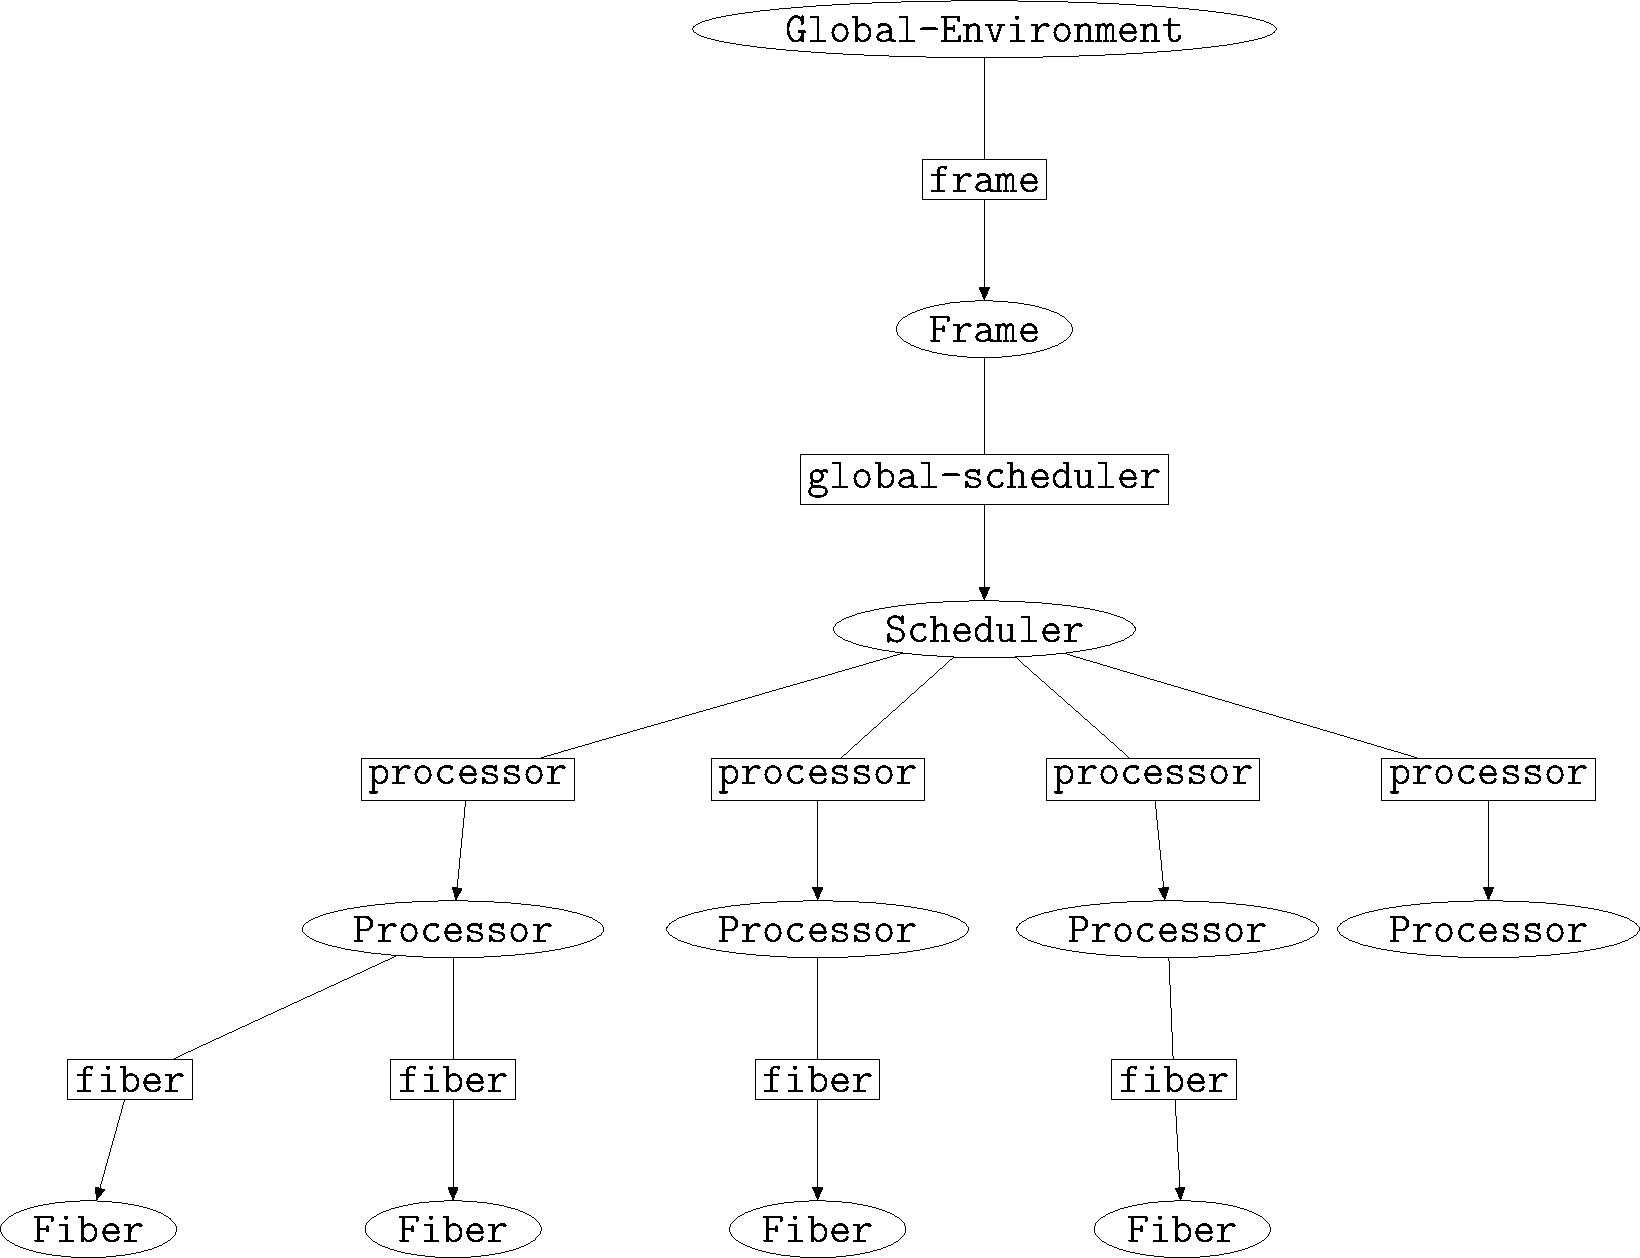
\includegraphics[width=12cm]{gfx/example_global_environment}
\caption[An example of a global environment with concurrent processors
  and parallel fibers.]{An example of a global environment with its
  frame object and a definition of the global scheduler object.  The
  global scheduler contains references to concurrent processors, which
  organize the parallel fibers, virtual machines that execute user
  programs.}
\label{figure:example_global_environment}
\end{figure}

\section{Stepping the Simulation State}

For the purposes of description and evaluation of the complexity of my
implementation of the reflective simulation, I assume that each
concurrent processor executes at the same speed and steps the
simulation forward at the same time.  Given a simulation state graph,
$S$, all of the concurrent processors step the simulation forward to
the next simulation state graph.
Equations\ \ref{equation:define_simulation_step_first}
and\ \ref{equation:define_simulation_step_last} define the initial
simulation state and recursive definition of the step function that
computationally creates the next simulation state graph.
\begin{align}
\label{equation:define_simulation_step_first}
    S[0] &\equiv \text{\emph{Initial simulation state graph}} \\
\label{equation:define_simulation_step_last}
  S[n+1] &= \text{step}(S[n])
\end{align}
Note that until this point, I have not previously introduced a
computational step function for the simulation state.  I have
previously defined the temporal transitions that compose $n$ layers of
distinct temporal orderings, one for each reflective layer in the
model, but these layers of temporal transition representations are
within the static state of the mind.  This computational step function
allows all of the previously described static structures to change to
new static representations.  The computational step function does not
exist within the mind, and the mind does not have any access to
symbolizing these different simulation state graphs that are now
introduced in the computational implementation.

Causally traced procedural reflection is the key component that allows
SALS to monitor changes to its own simulation state graph
representation.  Before discussing how procedural reflection must be
embedded into the definition of SALS' fundamental memory
representation, I must first briefly describe how fibers are
programmed in order to simulate simple non-reflective programs.

\section{Programming Language}

SALS includes a Lisp-like programming language, which is programmed
by typing statements that are called \emph{expressions}.  If
expression \ref{expression:print_hello} were typed into SALS, the
symbol ``green'' would be printed to the user's terminal screen.
\begin{equation}
\label{expression:print_hello}
\text{\tt [print `green]}
\end{equation}
The {\tt print} command is a useful debugging tool that can report
status messages to the programmer as the fiber reaches a specific
point in the program.

\section{Sequential and Parallel Programs}

SALS includes expressions for describing serial and parallel
programs.  For example, the expression
\begin{equation*}
\begin{array}{l}
\text{\tt [prog [print 1]} \\
\text{\tt ~~~~~~[print 2]} \\
\text{\tt ~~~~~~[print 3]]}
\end{array}
\end{equation*}
results in the output trace
\begin{equation*}
\begin{array}{l}
\text{\tt 1} \\
\text{\tt 2} \\
\text{\tt 3.}
\end{array}
\end{equation*}
The command {\tt prog} is a way for expressing a sequence of commands
to be executed in serial order.  SALS also includes the {\tt parog}
command for executing a list of commands in parallel, waiting for them
all to complete, and then continuing.
\begin{equation*}
\begin{array}{l}
\text{\tt [parog [print 1]} \\
\text{\tt ~~~~~~~[print 2]} \\
\text{\tt ~~~~~~~[print 3]]}
\end{array}
\end{equation*}
When {\tt parog} is used, it is unclear what command will complete
first because they are all running concurrently, in parallel, starting
at slightly different times.  Here is an example output trace from the
{\tt parog} expression:
\begin{equation*}
\begin{array}{l}
\text{\tt 3} \\
\text{\tt 1} \\
\text{\tt 2.}
\end{array}
\end{equation*}
The {\tt parog} expression is one way to easily start a number of
parallel fibers to simultaneously execute a number of different tasks
and wait for these tasks to complete.

\section{Fibers Create Objects}

SALS includes an object type system.  Every expression in SALS,
besides {\tt nil}, has an object type.  Objects in SALS are in most
cases based on a frame knowledge representation.  Objects have three
main classes of functionality: {\tt get}, {\tt set}, and {\tt have}.
The uses of these types of functionality are as follows:
\begin{itemize}
\item {\tt [get <object> <slot-name>]}

The object-oriented {\tt get} command retrieves the value from the
named slot of the object's frame.
\item {\tt [set <object> <slot-name> <new-value>]}

The object-oriented {\tt set} command mutates the value at the named
slot of the object's frame to be the given new value.
\item {\tt [have <object> <slot-name> <arguments>]}

The object-oriented {\tt have} command performs other types of
activities that are not simple frame slot accessors and mutators.  The
{\tt have} commands sometimes involve complex mutations or other
side-effects.
\end{itemize}

\section{Creating Parallel Fibers}

The {\tt apply} operator is the normal way for a SALS program to
evaluate a given function with arguments:
\begin{equation*}
\text{\tt [apply <function> <arguments>]}
\end{equation*}
The fundamental operator of SALS's parallel programming language is
the {\tt fiber} operator:
\begin{equation*}
\text{\tt [fiber <function> <arguments>]}
\end{equation*}
The {\tt fiber} operator does not evaluate the given function with
arguments.  The {\tt fiber} operator starts a new parallel fiber that
will evaluate the given function and arguments; the new fiber object
is returned.  The intermediate state or final result can be monitored
through the fiber object.

\section{Monitoring Simulated Activities}

SALS includes a tool named \emph{FiberMon} that is written in the SALS
programming language.  FiberMon helps the programmer to introspect on
all fibers currently in the simulation scheduler and is shown in
\autoref{figure:fibermon_many_fibers}.  Fibers may be easily removed
or added to the scheduler, which enables efficient scheduler
optimizations to be implemented at the highest levels of the language.
If any bugs arise in any parallel fiber, that fiber shows up in red in
the monitoring application, so that it may be inspected and debugged
by hand.
\begin{figure}[bth]
  \center
  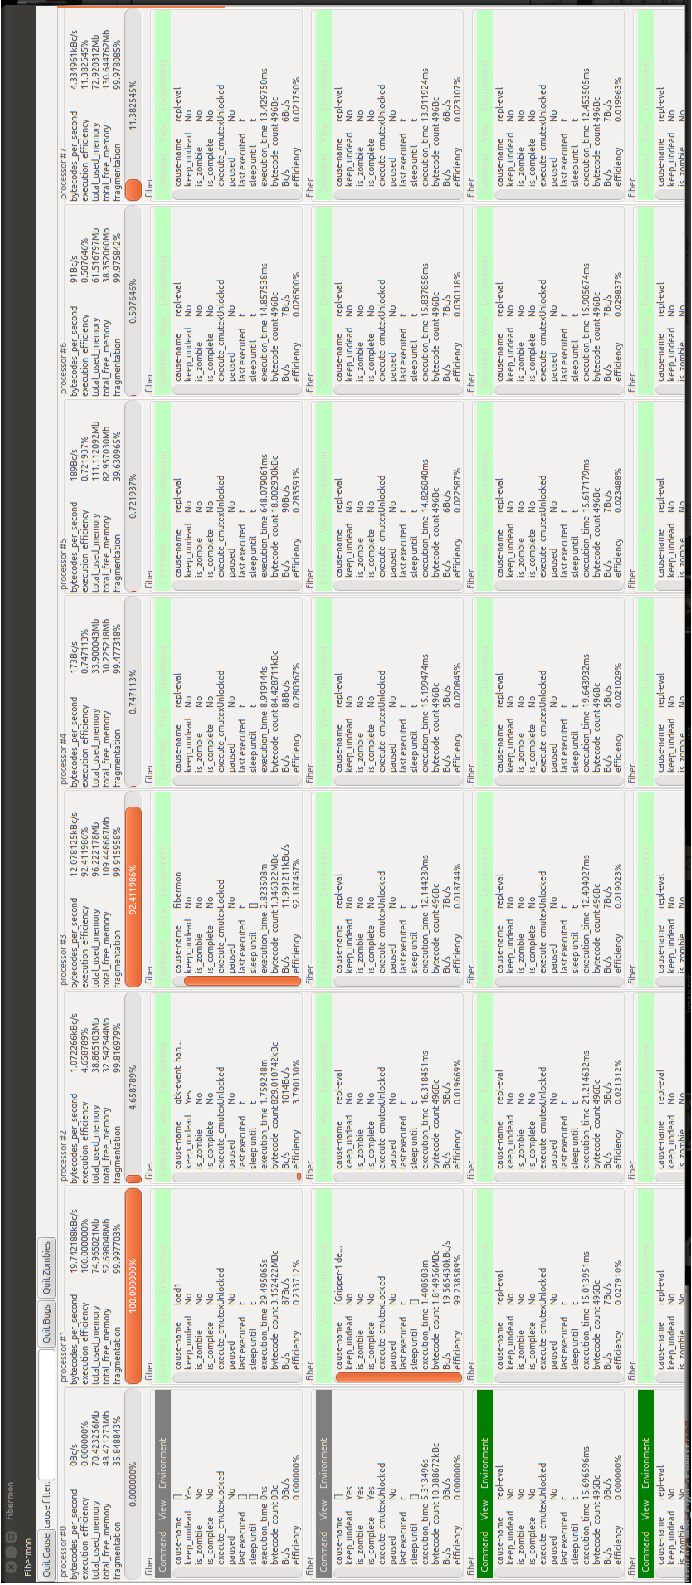
\includegraphics[width=10cm]{gfx/fibermon_many_fibers}
  \caption[FiberMon application monitoring many fibers]{FiberMon
    application monitoring hundreds of parallel fibers, simulated
    activities in Duration, executing on eight different physical
    processor cores.}
  \label{figure:fibermon_many_fibers}
\end{figure}

\section{Pausing and Resuming Activities}

SALS includes a {\tt pause} command to pause the current fiber:
\begin{equation*}
\text{\tt [pause]}
\end{equation*}
The {\tt pause} command causes the executing fiber to remove itself
from the scheduler, after removing itself, it yields the rest of the
scheduler cycle.  A fiber that is paused in this sense uses none of
SALS's processor resources because it is completely removed from
the scheduler.

If a fiber has paused, it cannot restart itself.  In order for a fiber
to resume execution, another executing fiber must use the
{\tt resume} command with the fiber object as an argument:
\begin{equation*}
\text{\tt [resume <fiber>]}
\end{equation*}

The {\tt pause} and {\tt resume} commands are extremely efficient for
managing large simulations in which most fibers will be inactive at
any given time, but they are a little cumbersome, so I have written a
lightweight and helpful \emph{fiber trigger} object, which I will
explain after explaining one more object that is used to program fiber
triggers.

\section{Mutual Exclusion}

SALS provides a primitive object called a \emph{mutex} for handling
the mutually exclusive access to resources.  A mutex object has two
possible states: locked and unlocked.  If the mutex object is unlocked
then when a fiber tries to locks the mutex, the mutex switches to the
locked state and the fiber continues execution.  If the mutex object
is already locked when a fiber tries to lock the mutex, the fiber will
pause until the mutex is unlocked, at which point the mutex will be
locked and the waiting fiber will resume execution.  Mutexes are used
for protecting shared resources from being used by more than one fiber
at a time.

Mutexes are a special type of object that must be supported by the
hardware of a concurrent computer.  Almost every parallel programming
language has a mutex construct that derives from this hardware mutex.
So, mutexes are common to parallel programming, but they are
notoriously difficult to debug, resulting in bugs affectionately
referred to as ``race conditions'' or ``deadlocks''.  In order to help
with debugging these types of problems, mutexes in SALS keep track of
which fibers are waiting for the lock or holding the lock.  I have
found this extra information invaluable in debugging complicated mutex
related bugs.

\section{Fiber Triggers}

The fiber trigger organizes sets of paused fibers so that they can be
woken up at the same time.  Basically, the fiber trigger is an object
that provides a useful abstraction for controlling fiber execution
that combines a mutex with the {\tt pause} and {\tt resume} commands.

A fiber can be added to the resume set of a fiber trigger by using the
{\tt wait-for-trigger} command as in the following example:
\begin{equation*}
\text{\tt [wait-for-trigger <fiber-trigger>]}
\end{equation*}
The {\tt wait-for-trigger} command atomically pauses the current fiber
and then adds the fiber to resume queue of the fiber trigger object.


%\section{leftovers...}

%\section{Symbols and Simulated Symbols}

%It becomes important at this point to keep track of the layer of
%modelling that results when one simulates thinking.  The danger is in
%losing an awareness of the difference between what one is thinking and
%what a simulation is simulating as thought.  For example, a programmer
%types symbols to express commands to the computer in a programming
%language.  These symbols have grounding for the programmer.  The
%computer continually repeats the same symbolic manipulation function,
%the combinational device.  So, when the simulation appears to create
%new symbols by manipulating the symbols contained within its
%programming, this is an illusion.  The observer of output from the
%simulation may create new symbols, but the computational process only
%has grounding in terms of the symbols of its programming.  Therefore,
%I will use the previously introduced asterisk notation for referring
%to different classes of simulated modelling.

%Now that I have described the difference between the symbols the
%programmer types and the symbols* that the AI simulates as being
%created, the first goal of my description of the implementation is to
%describe how SALS simulates the creation of a symbol.  The rest of
%this chapter will cover the creation of a symbol*, but first, I must
%discuss how the activities in Duration begin simulating by programming
%lists of symbols into SALS' interactive programming language.

%
%\section{Fiber Complete and Bug Found Triggers}
%
%get fiber triggers from fiber objects.
%
%execution complete versus bug found.
%
%
%\section{{\tt par-fib}}
%
%\begin{equation*}
%\begin{array}{l}
%\text{\tt [defunk par-fib [n]} \\
%\text{\tt ~~[if [== n 0]} \\
%\text{\tt ~~~~~~0} \\
%\text{\tt ~~~~[if [== n 1]} \\
%\text{\tt ~~~~~~~~1} \\
%\text{\tt ~~~~~~[let [[x []]} \\
%\text{\tt ~~~~~~~~~~~~[y []]]} \\
%\text{\tt ~~~~~~~~[parog [= x [par-fib [- n 2]]]} \\
%\text{\tt ~~~~~~~~~~~~~~~[= y [par-fib [- n 1]]]]} \\
%\text{\tt ~~~~~~~~[+ x y]]]]]}
%\end{array}
%\end{equation*}
%
%
%\section{Symbolic Statements in SALS}
%
%\section{Three Categories of Symbol}
%
%SALS programming expressions are combinations of symbols in lists.
%It is important to keep all of these symbols straight.  I have so far
%introduced three slightly different conceptions of symbols: (1) the
%symbols that are reflectively symbolized from the activities of
%Duration, (2) the symbols that a programmer types into a computer, and
%(3) the simulated symbols that are generated by the simulated
%first-order reflective layer of thinking.
%
%\section{Concurrent Memory Allocation Pools}
%
%SALS works off of a multiple pool memory allocation system that
%allows separate pools for each concurrent virtual processor,
%eliminating the need for many lock situations that occur with shared
%memory pools.
%
%\section{Garbage Collection}
%
%
%
%\section{Layered Cognitive Architecture}
%
%On this computational substrate, I have built a layered cognitive
%architecture that is inspired by Minsky's description of the bottom
%four layers of his Emotion Machine, or Model-6 architecture.  This
%includes, a physical world, a reactive mapping of the physical world
%to pre-symbolic activities, a first-order reflective thinking layer
%that creates symbols, causal models, and plans for accomplishing
%physical goals, as well as a second-order reflective thinking layer
%that creates symbols, causal models, and plans for accomplishing
%first-order thinking goals.  The model behind this implementation
%inductively explains how this implementation can be extended to an
%arbitrary number of reflective thinking layers.  While this part of
%the thesis is primarily focused on the simulation of a static,
%modelled representation of this model, I derive the fundamental basis
%of my model of mind in non-technical English in
%\autoref{part:the_model}.
%
%\section{Block Building Domain}
%
%My architecture exists in three main parts: the physical layer, the
%first-order reflective layer, and the second-order reflective layer.
%In order to explain how my model allows for learning at multiple
%levels, I use a simulation of a physical domain that is easy to
%understand.  I use this simulation primarily for communication of my
%working model by demonstrating learning at multiple reflective levels
%in response to a single physical failure.
%
%My simulation of the physical block building domain is meant to appear
%as similar to the canonical toy problem, \emph{Blocks World}, with one
%key exception: my model is meant to have a different interpretation
%than the original Blocks World.  The primary point to emphasize here
%is that my physical simulation is meant to represent a dynamic
%physical world as opposed to the logical and completely static
%reference for the Blocks World physical domain.
%
%
%
%\section{Reactive Layer}
%
%The physical layer in my model is implemented by combining the
%physical simulation with a reactive layer that maps the physical
%simulator perceptual and motor functions to ``sub-symbolic''
%activities that are available to first-order reflection.




%%************************************************
\chapter{Causally Reflective Procedural Tracing}
\label{chapter:causally_reflective_procedural_tracing}
%************************************************

The parallel fiber virtual machines create, mutate, and read from
memory as they execute sequences of bytecodes.  At any given point,
the SALS memory system is static.  The current execution state of
every fiber is represented in the global environment.  In order for
SALS to be fully reflective on all of the procedural effects of any
given fiber, I introduce a technique that I call \emph{causal
  reflective tracing}.  Causal reflective tracing is simply a way of
defining variables that are specific to each fiber that can be used to
control the low-level memory access, mutation, and creation functions.
This allows one fiber within SALS to subscribe to the procedural trace
events of another fiber without receiving procedural trace events of
its own execution, which would lead to an infinite regress, halting
the system.  Further, because SALS is inherently a parallel processing
system, a given fiber will often start a number of child fibers that
handle part of the processing for the parent fiber.  When a new fiber
is created, the child fiber inherits the causal variable bindings of
its parent fiber, enabling the same procedural tracing options for the
child as well.  So, causal reflective tracing is one of the basic
tools for keeping track of which pieces of memory were created,
mutated, or read by which other fibers.

Creating procedural trace events for the execution of a given fiber
slows the fiber down by a constant factor.  This is an important point
to consider when evaluating the theoretical time complexity of
concurrent procedurally reflective control algorithms.

\section{Semantic Memory Focuses Reflective Tracing}

While causal reflective tracing focuses the procedural event tracing
to memory interactions of specific fibers, this still results in
millions of events to consider every real-time second of execution.
In order to further focus the reflective tracing focus to specific
objects within the SALS memory system, specific pieces of memory can
be marked as \emph{semantic memory}.  Semantic memory objects are
created, mutated, and accessed in roughly the same way as all of the
frame-based objects in the SALS memory system.  Semantic memory
objects provide event streams that can be subscribed to by a number of
different parallel listeners in different fibers.  The following code
example shows how frame-based objects with default slot values and
constructors are used to define a {\tt Planning-Machine} type object:
\begin{equation*}
\begin{array}{l}
\text{\tt [deframe Planning-Machine [layer} \\
\text{\tt ~~~~~~~~~~~~~~~~~~~~~~~~~~~~[focus ~~~~~~~~~nil]} \\
\text{\tt ~~~~~~~~~~~~~~~~~~~~~~~~~~~~[execute ~~~~~~~nil]} \\
\text{\tt ~~~~~~~~~~~~~~~~~~~~~~~~~~~~[register-a ~~~~nil]} \\
\text{\tt ~~~~~~~~~~~~~~~~~~~~~~~~~~~~[register-b ~~~~nil]} \\
\text{\tt ~~~~~~~~~~~~~~~~~~~~~~~~~~~~[register-c ~~~~nil]} \\
\text{\tt ~~~~~~~~~~~~~~~~~~~~~~~~~~~~[positive-goals nil]} \\
\text{\tt ~~~~~~~~~~~~~~~~~~~~~~~~~~~~[negative-goals nil]]} \\
\text{\tt ~~[new [initial-layer]} \\
\text{\tt ~~~~[= layer initial-layer]} \\
\text{\tt ~~~~nil]]}
\end{array}
\end{equation*}
Once a frame-based object is defined, the ``{\tt new}'' operator is
used in order to create a new instance of the object type as in the
following example:
\begin{equation*}
\begin{array}{l}
\text{\tt [new Planning-Machine `Reflective-1]} \\
\end{array}
\end{equation*}

\section{Forgetful Event Streams}

By default, when there are no listeners to the procedural event
streams of a semantic frame-based object, no reflective events are
created, allowing the use of the object to run at full speed.  When a
listener subscribes to the procedural use of a specific semantic
memory object, events are added to ordered streams for the listening
subscribers.  In order to conserve memory resources, when multiple
parallel listeners are subscribed to a given event stream, only those
events that have not already been seen by all of the subscribers are
remembered.  Once all subscribers have processed an event, all events
before this event are forgotten.  This type of memory conserving event
stream is referred to as a \emph{forgetful event stream}.  In this way
semantic frames report the addition and removal of slot values to
reflective forgetful event stream subscribers.

\section{Semantic Knowledge-Bases}

Because it becomes awkward to subscribe to each an every frame-based
object that may be interesting to the reflective focus, semantic
frames that are created by specific fibers can be added to collections
of semantic frames that are called \emph{semantic knowledge-bases}.
Semantic knowledge-bases are good for organizing entire layers or
subsets of reflective layers that contain different types of semantic
frames.  Semantic knowledge-bases allow the same forgetful event
stream subscription services as semantic frames with the additional
capability of tracing the addition and removal of entire semantic
frames to and from the knowledge-base.

\section{Reflectively Reconstructed Semantic Knowledge-Bases}

Each parallel subscriber to the reflective procedural knowledge-base
events receives each event slightly after it occurs.  It often becomes
necessary to be able to refer to the historical state of the
knowledge-base under the reflective focus.  However, in order to not
slow down the primary procedure, the primary knowledge base must be
allowed to change during the time that it takes the reflective process
to process each event.  In this case, it becomes necessary to maintain
accurate reflective reconstructions of knowledge-bases that are
accurate at the reflective time of each reflective event that is
processed in parallel.  For example, in order to implement symbolic
perception, each slot value addition to the physical knowledge-base is
reflectively traced and the physical knowledge base is constructed as
a reflective copy that is accurate to the reflective time.  This
\emph{reflectively reconstructed semantic knowledge-base} is used to
perform a check of the immediate frame-based graph surroundings of the
change to see if one of the symbolic perceptions has become active or
inactive due to the change.

\section{Semantic Event Interval-Tree Knowledge-Bases}

While knowledge-base reconstructions are extremely fast to reference,
$O(1)$, they require a duplication of the memory requirements of the
focus knowledge base for every different point in time that is
required.  In order to allow efficient access of the state of
knowledge-bases at arbitrary points in the past, \emph{semantic event
  interval-tree knowledge-bases} are another type of representation
that is reflectively maintained without slowing down the procedure
under reflective focus.  A semantic event knowledge-base stores a type
of semantic frame that represents when a given semantic frame has a
specific slot value called a \emph{semantic event}.  A semantic event
is a semantic frame is an interval that spans a time from a beginning
time and an ending time, each of which may or may not be specified.
Semantic event knowledge-bases are reflectively traced and the
knowledge is always stored in two different representations, the basic
semantic event frames as well as a balanced interval tree that always
represents the current state of the semantic event knowledge-base.
The balanced interval tree allows accessing the state of the focus
knowledge-base in $O(log n)$ time, where $n$ is the number of events
stored in the semantic event knowledge base.  Although the time
complexity is not as efficient as the constant, $O(1)$, access time of
the reflectively reconstructed semantic knowledge-base, the semantic
event interval-tree knowledge base only requires $O(n)$ memory
complexity in order to allow access to the structure of the
knowledge-base at any point in the past, where $n$ is the number of
semantic events.

\section{Implemented Mind Monitoring Application}

{\mbox{\autoref{figure:implemented_mindmon}}} shows the implemented
MindMon application.
\begin{figure}
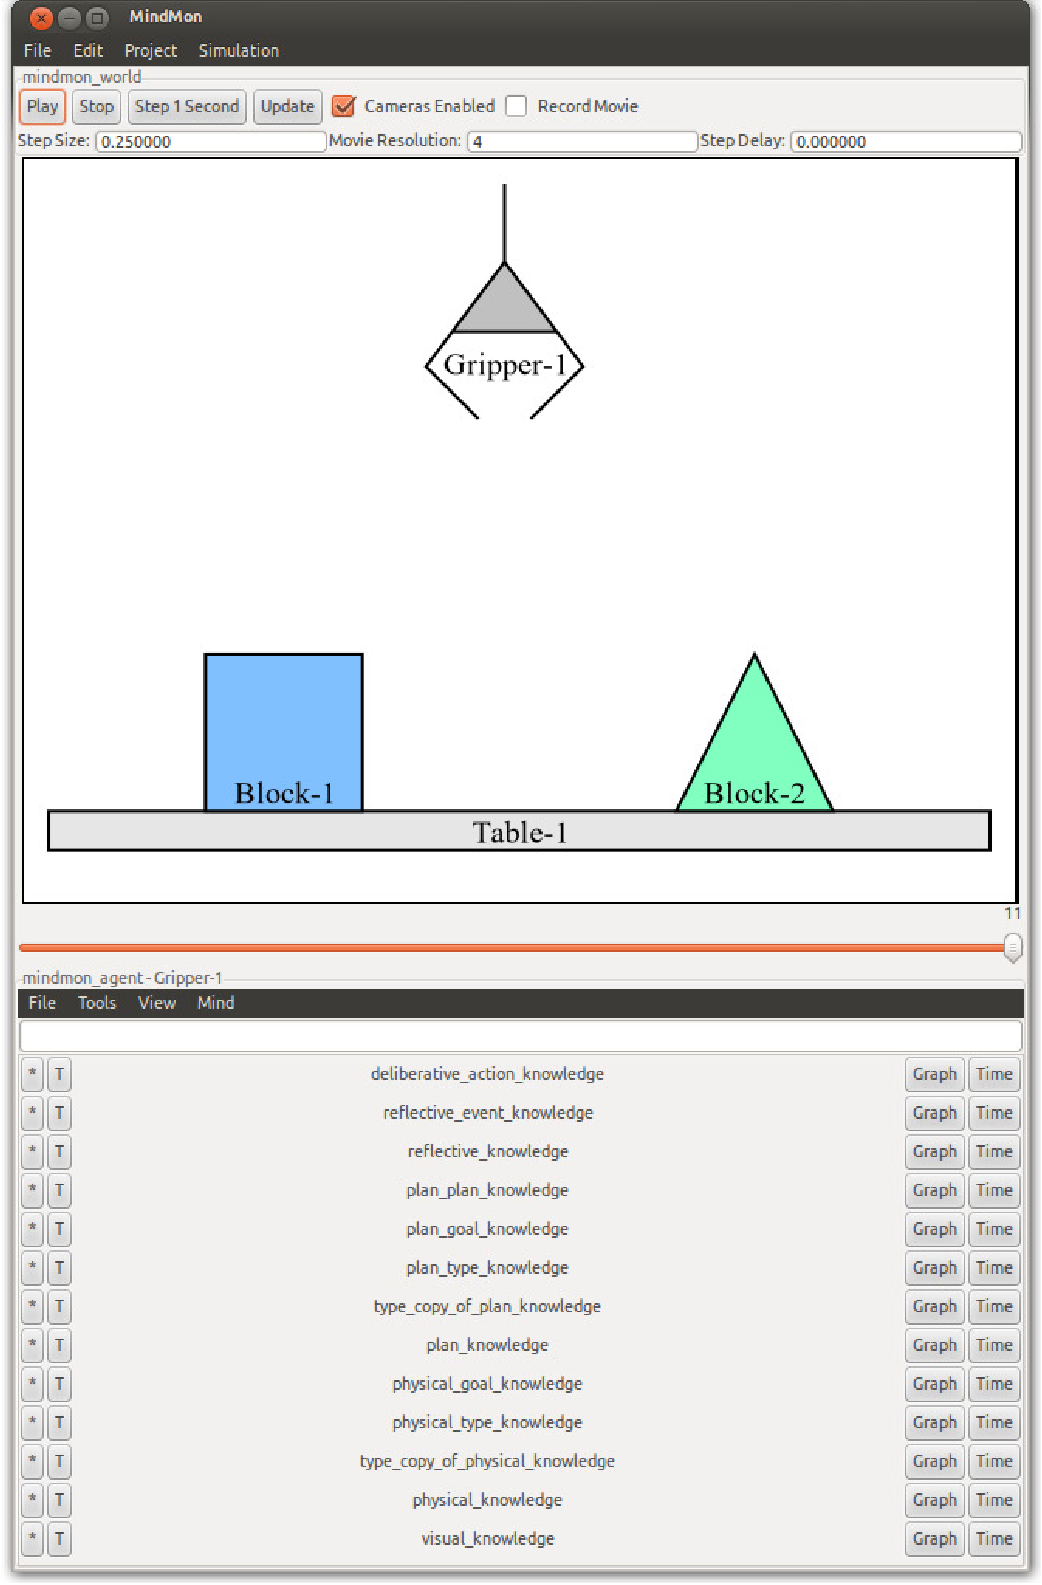
\includegraphics[width=10cm]{gfx/implemented_mindmon}
\caption[The implemented mind monitoring application, MindMon.]{The
  implemented mind monitoring application, MindMon.}
\label{figure:implemented_mindmon}
\end{figure}

\section{Implemented Physical Knowledge}

{\mbox{\autoref{figure:implemented_physical_knowledge}}} shows the
implemented physical knowledge.
\begin{figure}
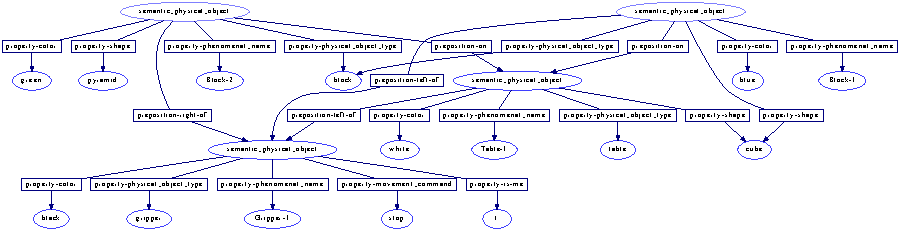
\includegraphics[width=10cm]{gfx/implemented_physical_knowledge}
\caption[The implemented physical knowledge.]{The implemented physical
  knowledge.}
\label{figure:implemented_physical_knowledge}
\end{figure}

\section{Implemented Semantic Event Knowledge-Base}

{\mbox{\autoref{figure:implemented_semantic_event_knowledge_base}}} shows the
implemented semantic event knowledge base.
\begin{figure}
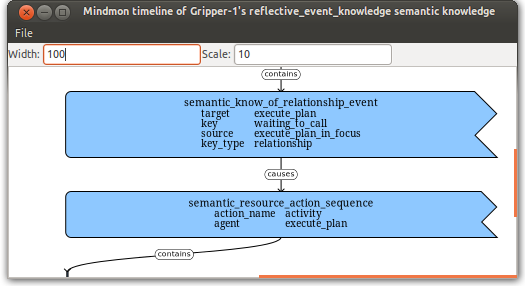
\includegraphics[width=10cm]{gfx/implemented_semantic_event_knowledge_base}
\caption[The implemented semantic event knowledge base.]{The
  implemented semantic event knowledge base.}
\label{figure:implemented_semantic_event_knowledge_base}
\end{figure}

\section{Implemented First-order Resource Activator}

{\mbox{\autoref{figure:implemented_first_order_resource_activator}}}
shows the implemented first-order resource activator.
\begin{figure}
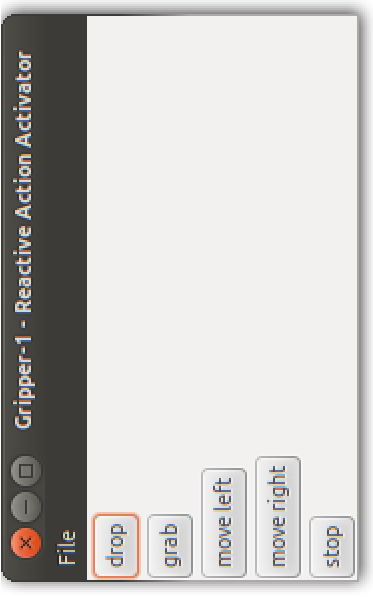
\includegraphics[width=10cm]{gfx/implemented_first_order_resource_activator}
\caption[The implemented first-order resource activator.]{The
  implemented first-order resource activator.}
\label{figure:implemented_first_order_resource_activator}
\end{figure}


%%************************************************
\chapter{The Mind Monitor Application}
\label{chapter:the_mind_monitor_application}
%************************************************

In order to control the SALS model of mind, a mind monitoring
application called \emph{MindMon} has been implemented.  MindMon is
based on abstract physical world and reflective thinking components
that allow reflective thinking layers to be interchanged with
different $\text{reflective}^0$ physical layers.  In this dissertation
I focus on a block building domain in order to demonstrate
second-order reflective learning to plan, but other more complex
physical domains have also been developed within SALS such as the
IsisWorld physical simulator described by \cite{smith:2010}, where
MindMon allows attaching multiple reflective thinking models to a
shared $\text{reflective}^0$ physical layer, a type of simulation that
assumes a more complex subjective philosophy of mind that is not
assumed in the non-subjective model described in
{\mbox{\autoref{part:the_model}}} of this thesis.
{\mbox{\autoref{figure:implemented_mindmon}}} shows the MindMon
application.
\begin{figure}
\hspace*{-1cm}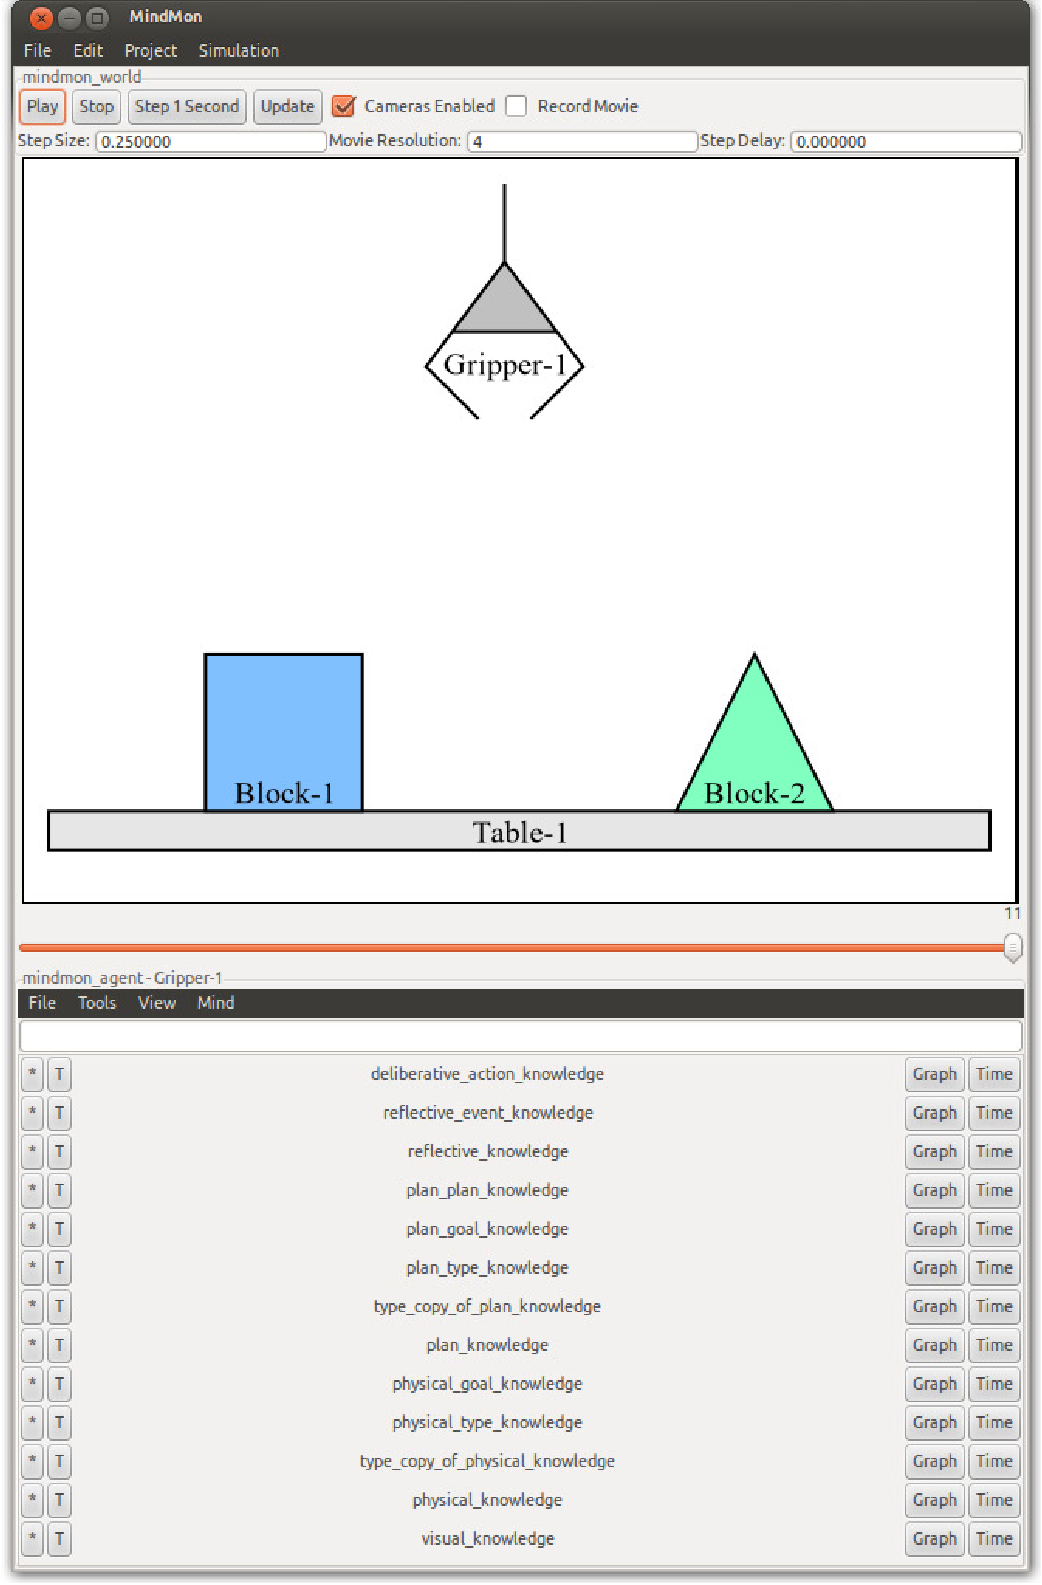
\includegraphics[width=13cm]{gfx/implemented_mindmon}
\caption[The mind monitoring application, MindMon.]{The mind
  monitoring application, MindMon, shown here with the simple block
  building domain and the reflective thinking layers described in this
  dissertation.}
\label{figure:implemented_mindmon}
\end{figure}

\section{The Physical Knowledge-Base}

The block building domain is a simulation based on two-dimensional
ridid-body physical laws, including floating point numerical
representations for object positions, velocities and accellerations.
These numerical representations and the processes that manipulate them
are part of the $\text{reflective}^0$ physical layer of the model, but
in order to focus the efficiency of the procedural reflection, a much
simpler relational graph representation has been specifically
represented in semantic frame-based objects in a semantic
knowledge-base, referred to as the \emph{physical knowledge-base}.
The physical knowledge-base includes objects with shapes, colors, and
multiple prepositional spatial relationships.
{\mbox{\autoref{figure:implemented_physical_knowledge}}} shows the
physical knowledge-base.
\begin{sidewaysfigure}
\begin{center}
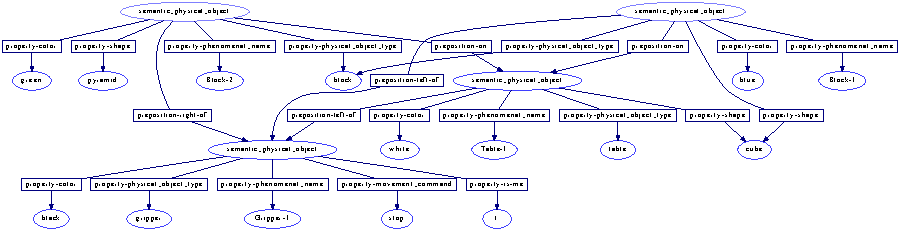
\includegraphics[width=24cm]{gfx/implemented_physical_knowledge}
\end{center}
\hspace{4cm}\parbox{15cm}{\caption[The physical knowledge-base.]{The
    physical
    knowledge-base.}\label{figure:implemented_physical_knowledge}}
\end{sidewaysfigure}

\section{Semantic Event Interval-Tree Knowledge-Base}

Semantic event interval-tree knowledge-bases are used for organizing
all of the remembered history of symbolic perceptions, symbolic
resource activations, as well as symbolic goal activation events.  The
version-space hypothesis concept learning algorithm
{\mbox{\cite[]{mitchell:1997}}} references these interval-tree
structures, which also contain other relevant information, such as
what compiled resource causes the activation of another resource.  In
this way, all interactions between built-in and learned reactive
resources are recorded.
{\mbox{\autoref{figure:implemented_reflective_event_knowledge_base}}}
shows an example overview of a large semantic event interval-tree
knowledge-base, while
{\mbox{\autoref{figure:implemented_semantic_event_knowledge_base}}}
shows a readable small part of an example semantic event interval-tree
knowledge-base.
\begin{figure}
\begin{center}
\hspace*{-2cm}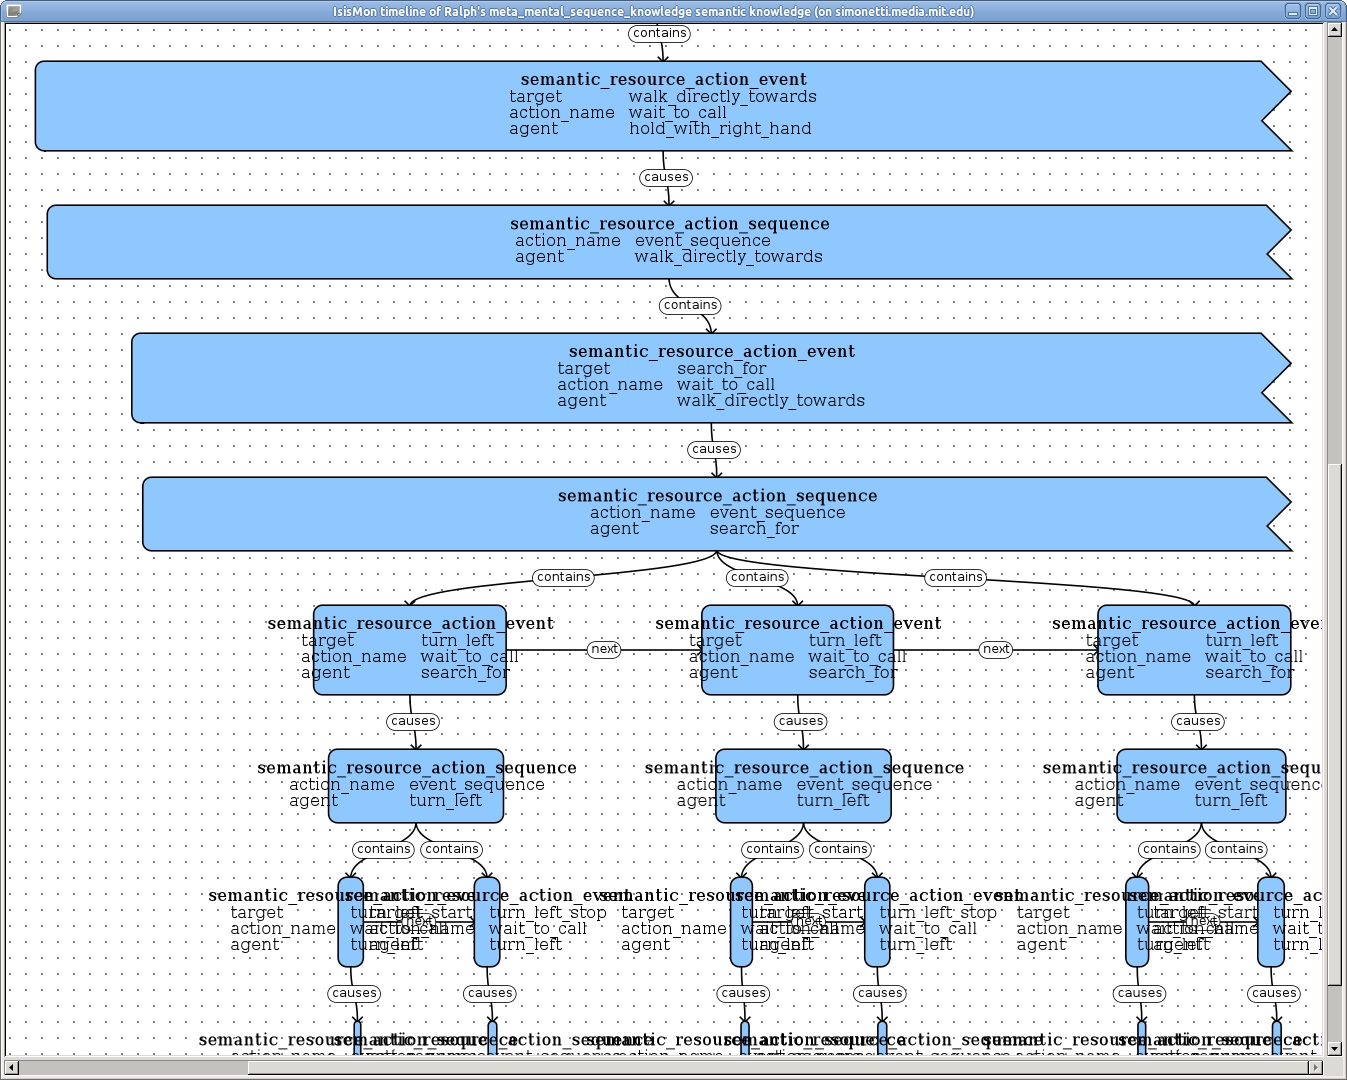
\includegraphics[width=13cm]{gfx/implemented_reflective_event_knowledge_base}
\end{center}
\caption[An example overview of a large semantic event interval-tree
  knowledge-base.]{An example overview of a large semantic event
  interval-tree knowledge-base.  See
  {\mbox{\autoref{figure:implemented_semantic_event_knowledge_base}}}
  for a readable view.}
\label{figure:implemented_reflective_event_knowledge_base}
\end{figure}
\begin{figure}
\begin{center}
\hspace*{-3cm}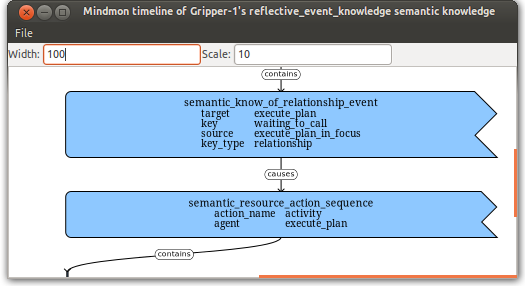
\includegraphics[width=15cm]{gfx/implemented_semantic_event_knowledge_base}
\end{center}
\caption[A close-up view of the semantic event interval-tree
  knowledge-base.]{A close-up view of the semantic event interval-tree
  knowledge-base.  Note the ``contains'' and ``causes'' extra semantic
  relationships between resource activation events.  Event sequences
  for one compiled resource contain sequential plan steps, while
  activations of parallel executing resources are shown as cause
  relationships.  See
  {\mbox{\autoref{figure:implemented_reflective_event_knowledge_base}}}
  for a more global perspective.}
\label{figure:implemented_semantic_event_knowledge_base}
\end{figure}

\section{First-order Resource Activator}

Every resource in SALS is available for user-interaction by using the
activators and monitors of the interchangeable reflective thinking
objects of the Mind Monitor application.  The SALS reflective thinking
layers have been tested with a number of interchangeable
$\text{reflective}^0$ physical layers.
{\mbox{\autoref{figure:implemented_first_order_resource_activator}}}
shows the simplest of these interchangeable $\text{reflective}^0$
physical layers, the built-in reactive symbolic resources of the block
building domain.
\begin{figure}
\begin{center}
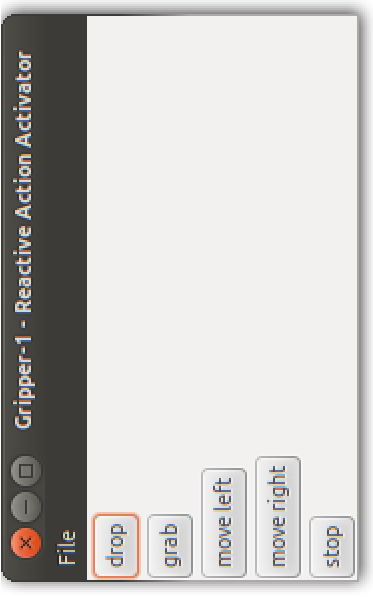
\includegraphics[width=8cm]{gfx/implemented_first_order_resource_activator}
\end{center}
\caption[The first-order resource activator.]{The first-order resource
  activator.}
\label{figure:implemented_first_order_resource_activator}
\end{figure}
%{\mbox{\autoref{figure:implemented_isisworld_first_order_resource_activator}}}
%shows the IsisWorld first-order resource activator.
%\begin{figure}
%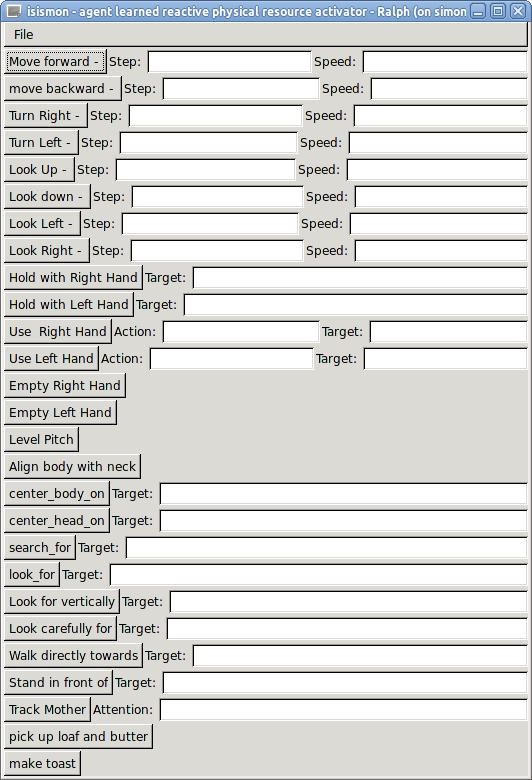
\includegraphics[width=11cm]{gfx/implemented_isisworld_first_order_resource_activator}
%\caption[The implemented IsisWorld first-order resource
%  activator.]{The IsisWorld first-order resource
%  activator.  These resources were by Jing Jian.}
%\label{figure:implemented_isisworld_first_order_resource_activator}
%\end{figure}

\section{First-order Planning Machine Knowledge}

{\mbox{\autoref{figure:implemented_planning_machine_knowledge_detailed}}}
shows a detailed view of the first-order planning machine
knowledge-base, while
{\mbox{\autoref{figure:implemented_first_order_planning_machine_knowledge}}} shows
a simpler view that shows only the planning machine registers.
\begin{sidewaysfigure}
\begin{center}
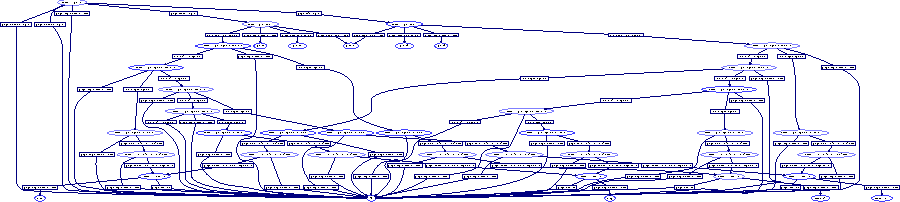
\includegraphics[width=24cm]{gfx/implemented_planning_machine_knowledge_detailed}
\end{center}
\hspace{4cm}\parbox{15cm}{\caption[A overview of the first-order
    planning machine knowledge-base.]{A overview of the first-order
    planning machine knowledge-base with two plans.  The small
    circular node in the far upper left represents the planning
    machine semantic object.  See
    {\mbox{\autoref{figure:implemented_first_order_planning_machine_knowledge}}}
    for a readable small portion of this same
    knowledge-base.}\label{figure:implemented_planning_machine_knowledge_detailed}}
\end{sidewaysfigure}
\begin{figure}
\begin{center}
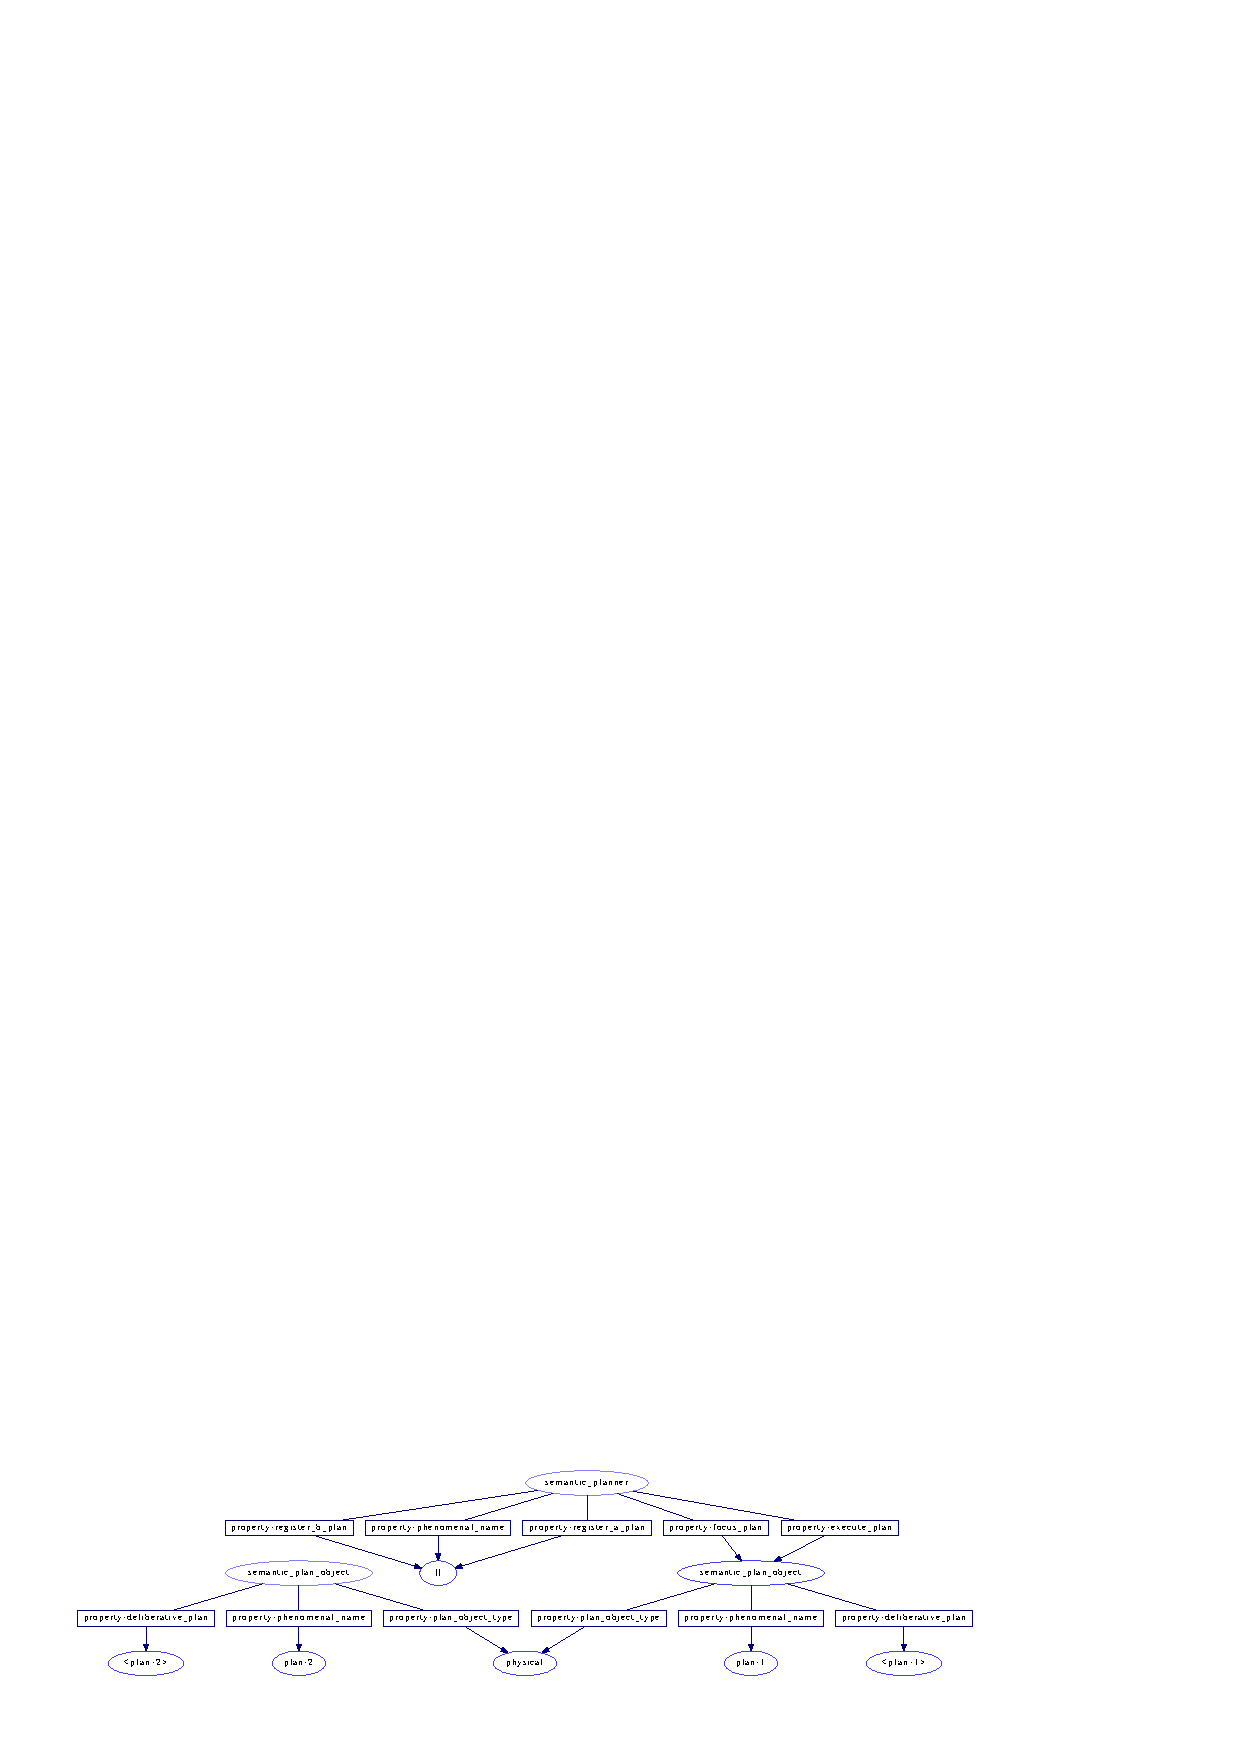
\includegraphics[width=14cm]{gfx/implemented_planning_machine_knowledge}
\end{center}
\caption[A small portion of the first-order planning machine
  knowledge-base.]{A small portion of the first-order planning machine
  knowledge-base that only shows the planning machine registers and
  plans without the details of their content.  See
  {\mbox{\autoref{figure:implemented_planning_machine_knowledge_detailed}}}
  for an overview of the entire knowledge-base.}
\label{figure:implemented_first_order_planning_machine_knowledge}
\end{figure}

\section{First-order Plan Activator}

{\mbox{\autoref{figure:implemented_first_order_plan_activator}}} shows
the first-order plan activator.
\begin{figure}
\begin{center}
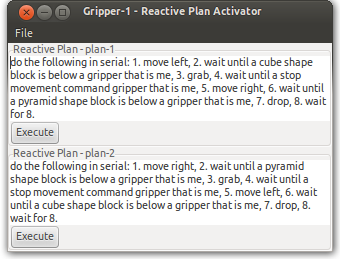
\includegraphics[width=10cm]{gfx/implemented_first_order_plan_activator}
\end{center}
\caption[The first-order plan activator.]{The first-order plan
  activator.}
\label{figure:implemented_first_order_plan_activator}
\end{figure}

\section{Second-order Resource Activator}

{\mbox{\autoref{figure:implemented_second_order_resource_activator}}}
shows the second-order resource activator.
\begin{figure}
\begin{center}
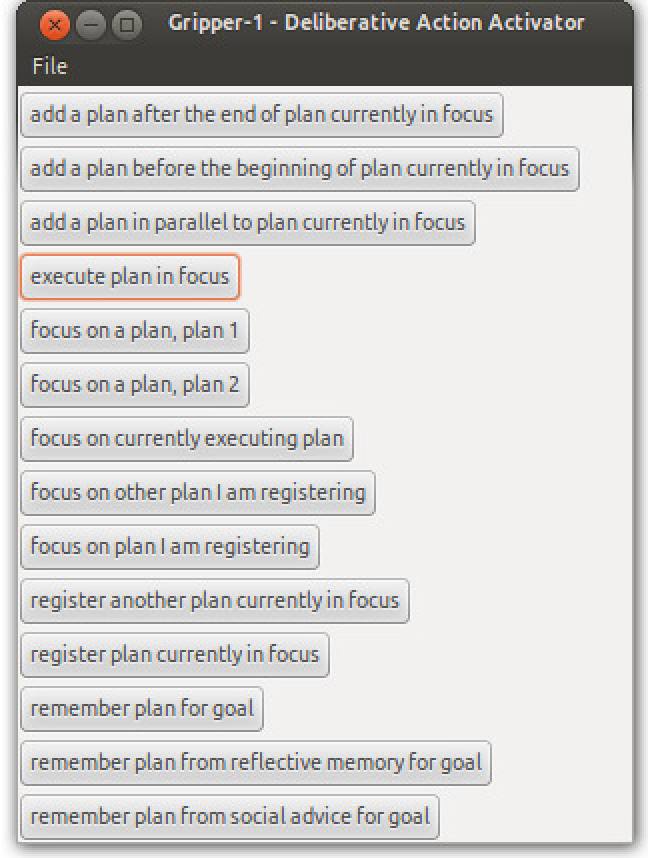
\includegraphics[width=10cm]{gfx/implemented_second_order_resource_activator}
\end{center}
\caption[The second-order resource activator.]{The second-order
  resource activator.}
\label{figure:implemented_second_order_resource_activator}
\end{figure}

\section{An Example Storyboard}

{\mbox{\autoref{figure:implemented_example_learning_storyboard}}}
shows a storyboarded example of second-order learning.
\begin{figure}
\begin{center}
\begin{tabular}{cc}
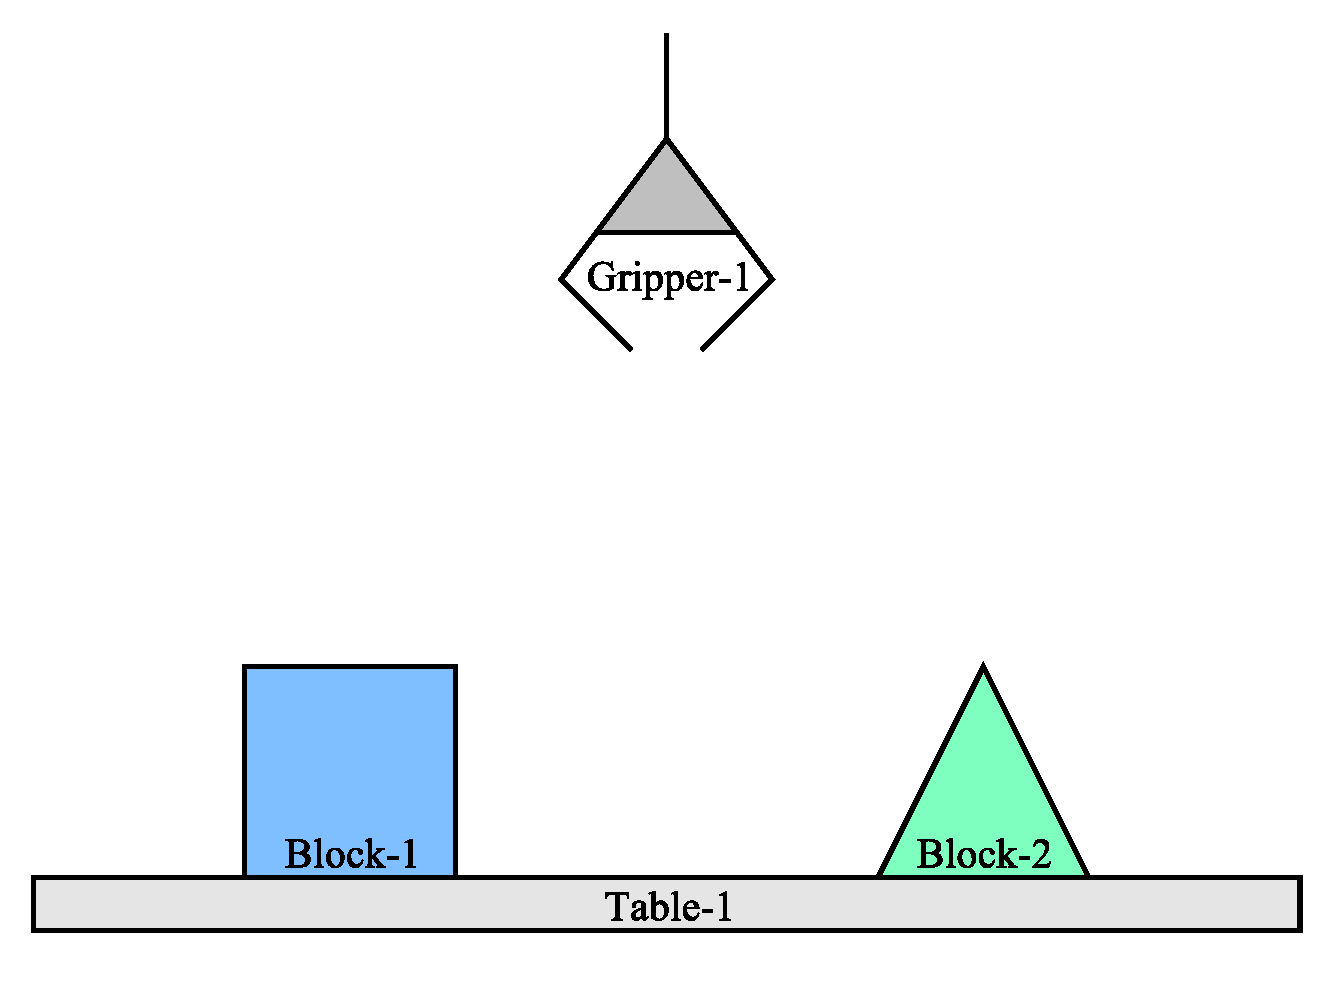
\includegraphics[width=4cm]{gfx/blocks_world_example-1} & 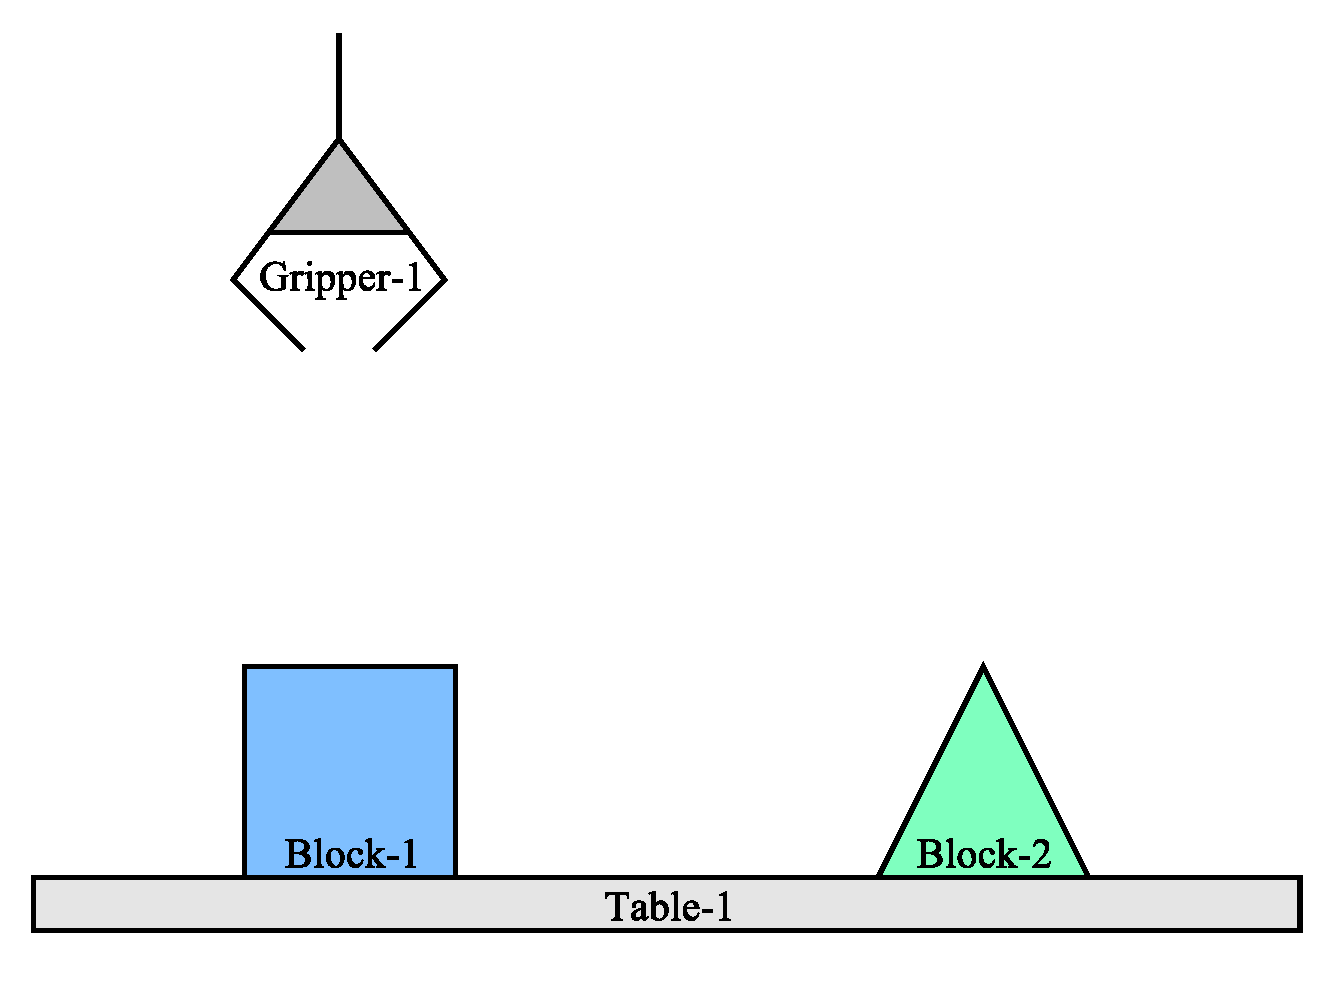
\includegraphics[width=4cm]{gfx/blocks_world_example-2} \\
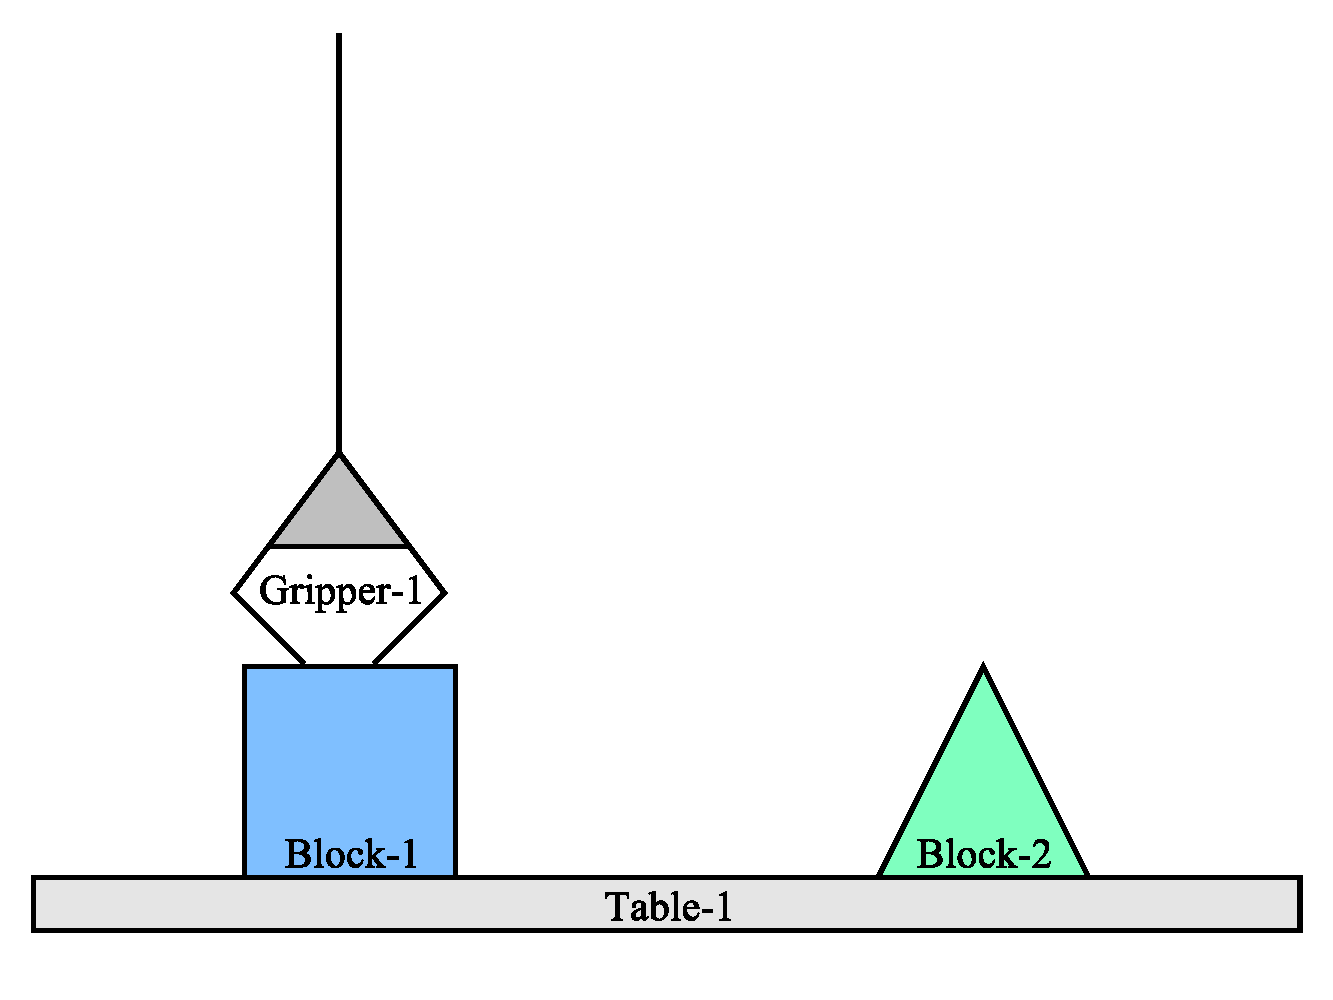
\includegraphics[width=4cm]{gfx/blocks_world_example-3} & 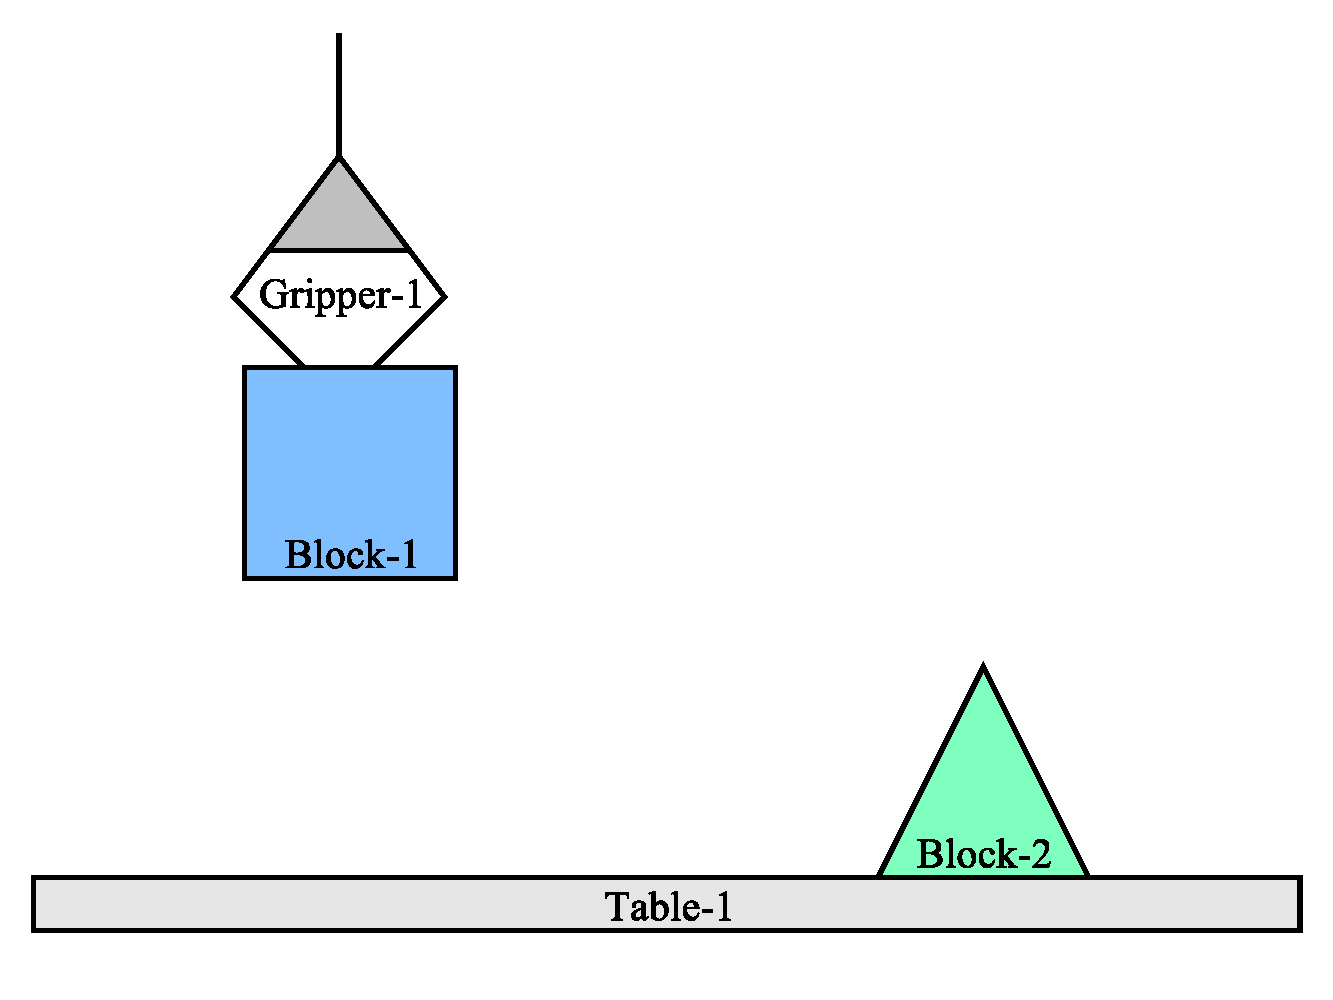
\includegraphics[width=4cm]{gfx/blocks_world_example-4} \\
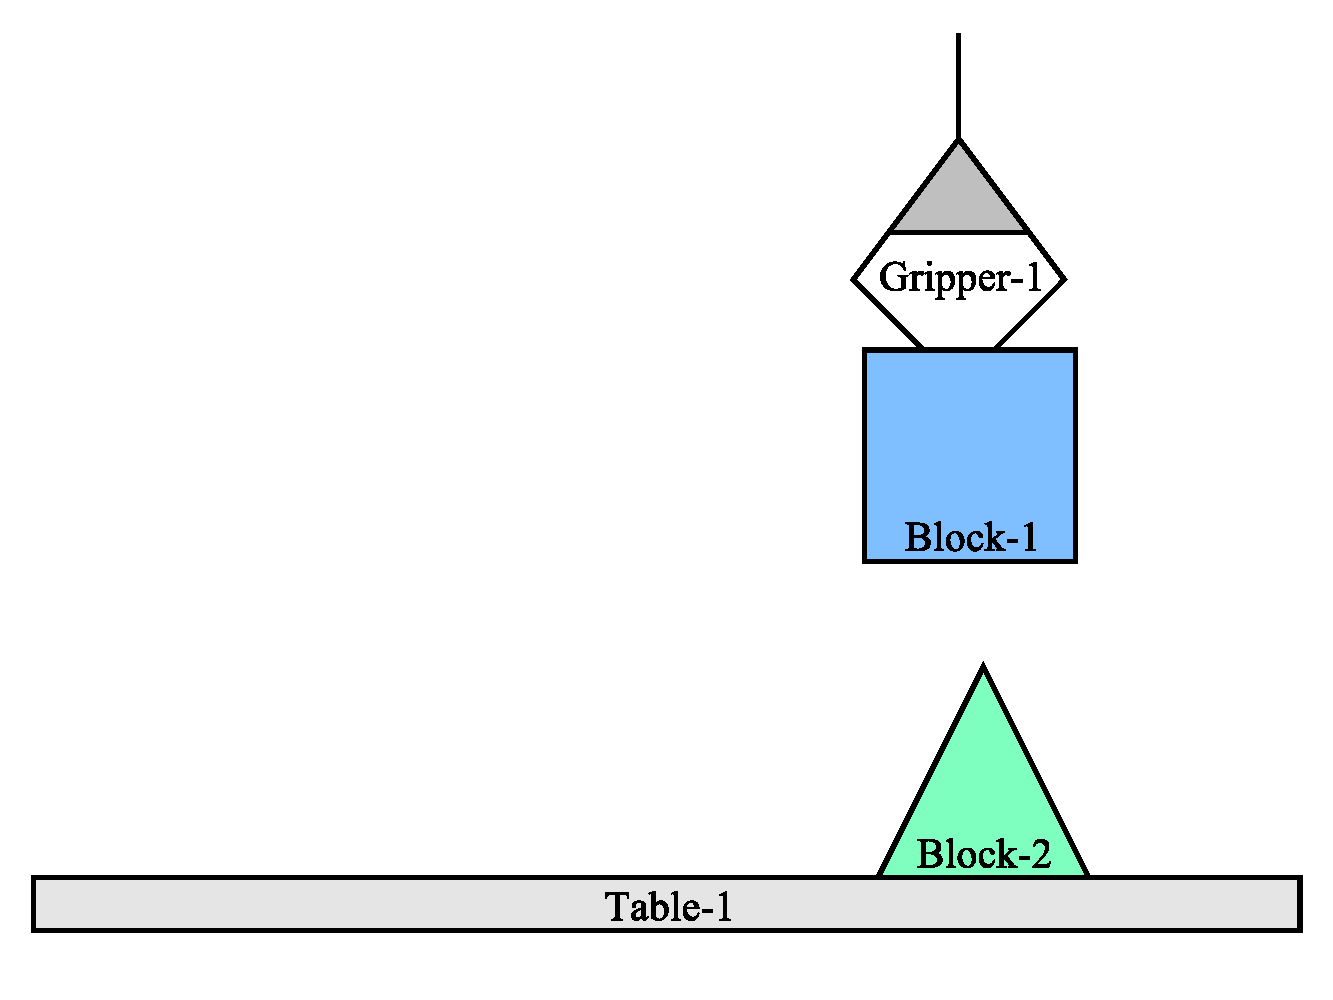
\includegraphics[width=4cm]{gfx/blocks_world_example-5} & 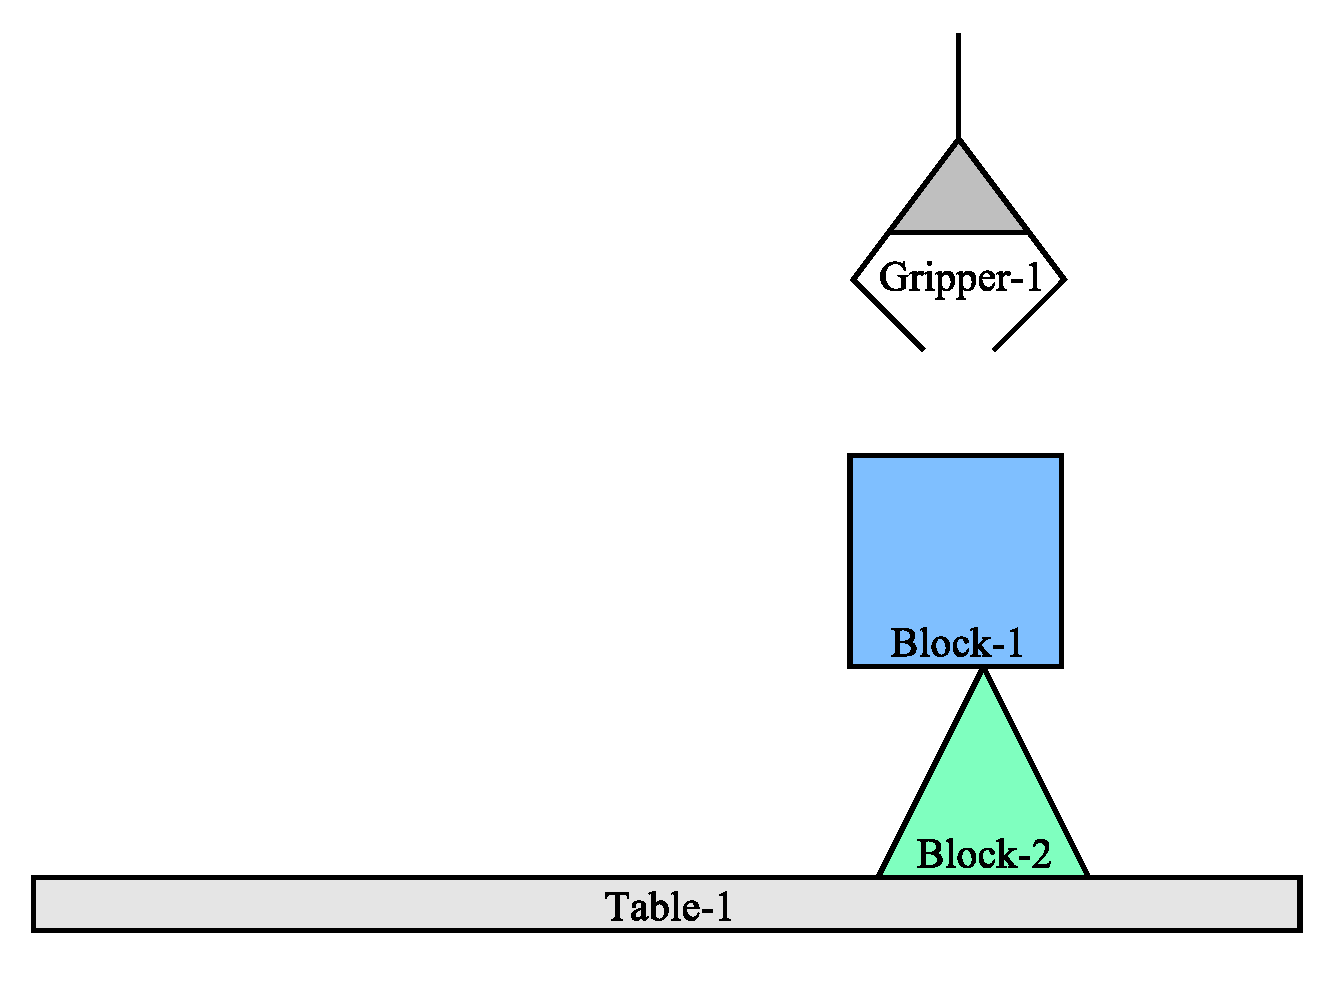
\includegraphics[width=4cm]{gfx/blocks_world_example-6} \\
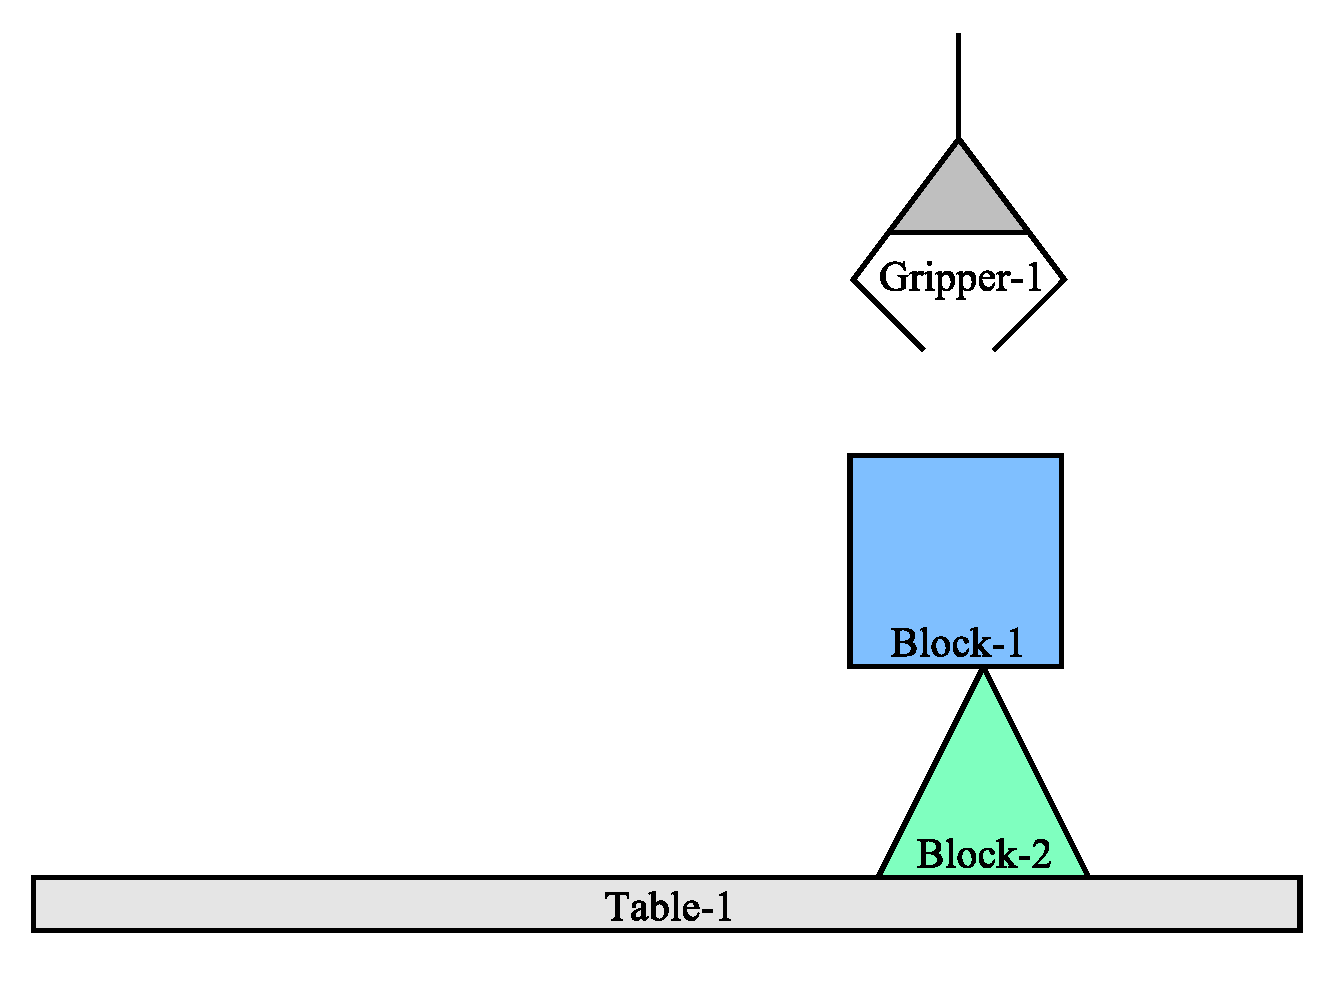
\includegraphics[width=4cm]{gfx/blocks_world_example-7} &  
\end{tabular}
\end{center}
\caption[A storyboarded example of second-order learning.]{A
  storyboarded example of second-order learning.}
\label{figure:implemented_example_learning_storyboard}
\end{figure}

%%*****************************************
\chapter{Related Implementations}
\label{chapter:related_implementations}
%*****************************************



%\cleardoublepage\part{The Simulation}\label{part:the_simulation}
%%************************************************
\chapter{Introducing Simulation}
\label{chapter:introducting_simulation}
%************************************************

Keeping distinctions between the continuous dynamic referent and
discrete static symbols, a model can be constructed which allows $n$
layers of reflection to be described.  Non-reflective AI models learn
by correcting one immediate cause of a failure; however, given a
layered model, New opportunities for considering one failure to also
be failures in the reflective layers ``above'' and ``below'' the
original failure can be described, resulting in an arbitrary number of
reflective learning opportunities from a single failure.

I will not attempt to give a complete representation for a general
problem domain nor a complete description of a general problem solver.
My work here leaves the unmodellable as known to be just that.
Thinking as a dynamic activity uses models as useful tools with the
clear understanding that these models are static.  Further, and
critically important for the advancement of the field of AI, when
describing reflective thinking, it is imperative to have an explicit
awareness of thinking being limited to manipulating the static.  I
will therefore refer to an AI model as simply an ``AI'' with the
shared understanding that I am referring to a static model.

The simulation model is an extension of the model of mind that
includes a mathematical description of a discrete ``state'' of the
model in a discrete time.  Neither the model of mind nor the
simulation model changes over time.  The simulation model therefore
makes reference to a discretely stepped state that is used to simulate
the necessarily separate, static model of mind.  The term
``simulation'' is thus used as a general reference to the dynamic
activity in Duration that manipulates and steps the state of the
simulation model.  In describing the simulation model, it is important
to not confuse the dynamic activity of simulation with the model or
the state of the model, which are both static at any given point in
time.  The term ``simulation'' is the only reference to activities in
Duration.  This distinction is necessary for the simulation model to
not be limited to simulating a specific kind of activity.

For example, consider a simulation of topological proof.  A
mathematician can ``simulate'' the rules of topological proof by first
seeing a static arrangement of symbols on paper.  These symbols can be
manipulated in the process of proving or disproving the initial
topological statement.  There is no existing logical or mathematical
formulation of the activities of topological proof.  I describe how a
symbolic state space can be added to the model of mind for the
purposes of simulation.  How exactly this simulation is done is left
until the next part, where the activity of simulation is assumed to be
computational.

The activities in Duration in the model of mind exist prior to their
symbolization, and since it is obviously not possible to refer to
something prior to symbolizing it, the assumption that these
activities have already been symbolized is necessary in order to
mathematically describe the state of the simulation model.  Defining
the simulation model requires a description in terms of symbols for
the ``undescribed activities in Duration.''  Each assumption made in
symbolizing the ongoing activities in Duration restricts the
simulation model from being a model of those assumptions because only
the symbolic result of those assumptions is available for the
simulation of the activity of reflection.


%%************************************************
\chapter{Graph Notation}
\label{chapter:graph_notation}
%************************************************

\section{Dynamic Activities as a Set}

\begin{figure}
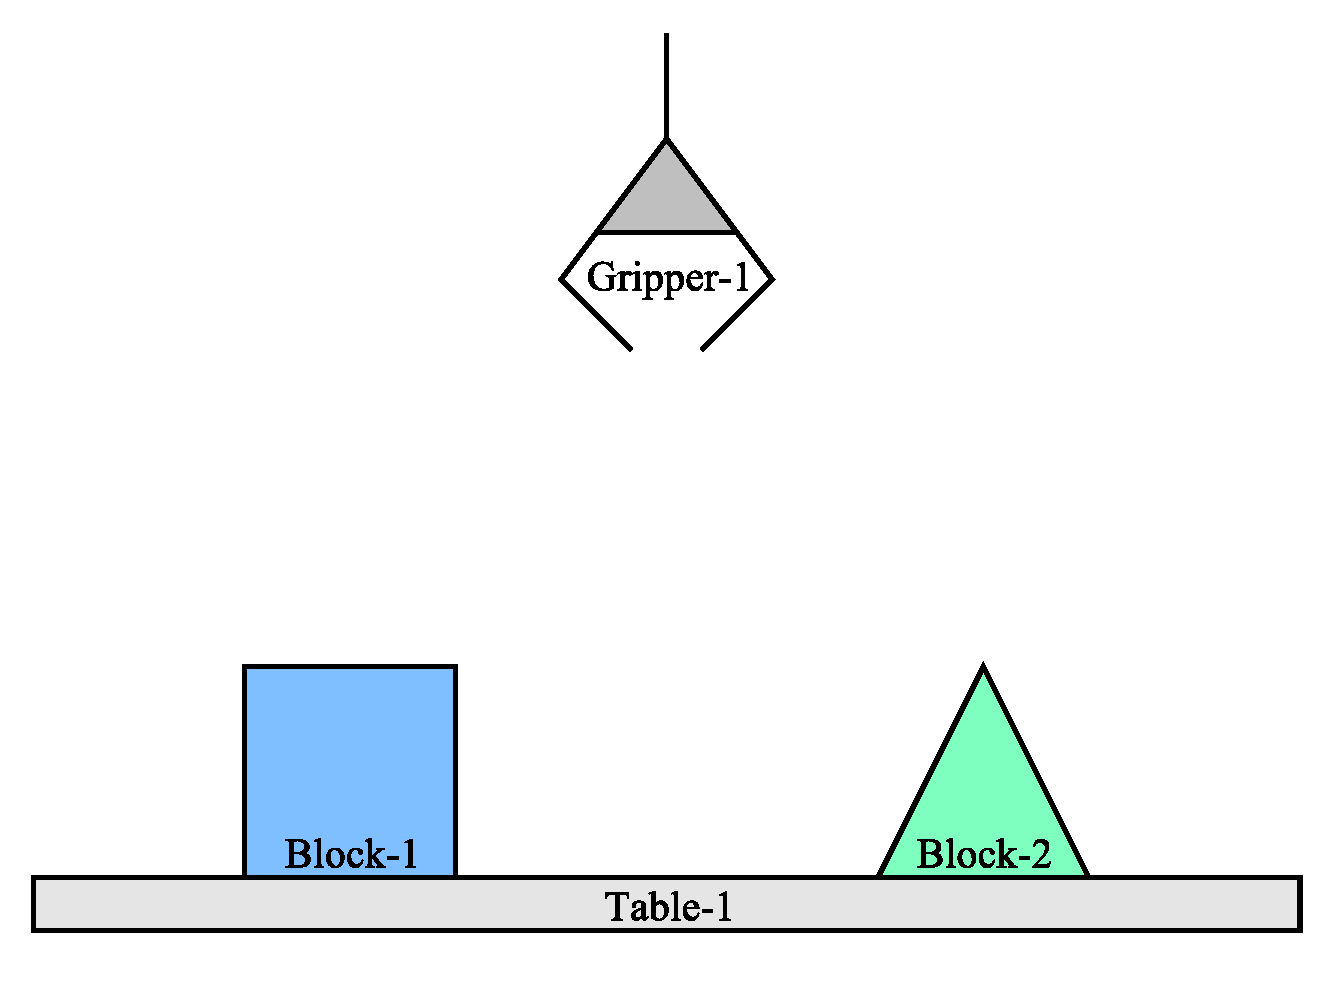
\includegraphics[width=10cm]{gfx/blocks_world_simulation}
\caption{An example for simulation.}
\label{figure:blocks_world_simulation}
\end{figure}

I will begin with one of the simplest mathematical models, a
\emph{set} of symbols, to model of the activities in Duration.  I will
first describe the simulation model as the mathematical set, X, the
activities of the state.  Here is an example of a possible
symbolization of the activities shown in
{\mbox{\autoref{figure:blocks_world_simulation}}}:
\begin{equation}
\label{equation:example_initial_state}
X =
  \left\{
    \begin{array}{l}
      \text{{\tt{Gripper-1}}}, \\
      \text{{\tt{Block-1}}}, \\
      \text{{\tt{Block-2}}}, \\
      \text{{\tt{Table-1}}} \\
      \text{{\tt{sitting-on}}}, \\
      \text{{\tt{being-above}}}, \\
      \text{{\tt{moving}}}, \\
      \text{{\tt{left}}}
    \end{array}
  \right\}
\end{equation}

\section{A Graph Representation}

The activities in Duration exist in a continuous Spatial arrangement
that is symbolized and ordered by the reflective thinking layers.  In
order to simulate this continuous homogenous Space, a discrete static
representation must be included in the state of the simulation model.
A graph of labelled nodes and edges can be used to represent the
activity of a Spatial relationship in the simulation.  Because the
graph provides a clear notation for referring to types of Spatial
arrangements of activities, a modified notation originally from
{\mbox{\cite{messmer:1995}}} is used to define a labelled graph in
{\mbox{Definition~\ref{definition:graph_first}}} and a labelled
subgraph in {\mbox{Definition~\ref{definition:graph_last}}}.

\begin{definition}
\label{definition:graph_first}
\emph{
A graph $G$ is the 4-tuple $(V, ~E, ~\mu, ~\nu)$, where
\begin{itemize}
\item $V$ is the set of vertices,
\item $E ~{\subseteq}~ V ~{\times}~ V$ is the set of edges,
\item $\mu : V \mapsto \{\ell_V\}$ is a function assigning a set of labels to each vertex.
\item $\nu : E \mapsto \{\ell_E\}$ is a function assigning a set of labels to each edge.
\end{itemize}
}\end{definition} \noindent In this definition, the edges are
directed, i.e. there is an edge from $v_1$ to $v_2$ if $(v_1,
v_2){\in}E$.  The empty graph, i.e. the graph with an empty set of
vertices will be denoted by $\emptyset$.  The union of the set of
labels referred to by $\mu$ and $\nu$ will be sometimes be referred to
with a dot notation, $\mathring{G}=\ell_V {\cup} \ell_E$.

\begin{definition}
\label{definition:graph_last}
\emph{ Given a graph $G = (V, E, \mu, \nu)$, a \emph{subgraph} of $G$
  is a graph $G_s = (V_s, E_s, \mu_s, \nu_s)$ such that
\begin{enumerate}
\item $V_s ~{\subseteq}~ V$
\item $E_s ~{\subseteq}~ V_s {\times} V_s$,
\item $\mu_s$ is the restriction of $\mu$, i.e.
\begin{align*}
\mu_s(e) &\subseteq
   {\left\{
      \begin{array}{ll}
        \mu(v)           & \text{if }v {\in} V_s \\
        \text{undefined} & \text{otherwise}
      \end{array}
    \right.}
\end{align*}
\item $\nu_s$ is the restriction of $\nu$, i.e.
\begin{align*}
\nu_s(e) &\subseteq
   {\left\{
      \begin{array}{ll}
        \nu(e)     & \text{if }e {\in} E_s \\
        \text{undefined} & \text{otherwise}
      \end{array}
    \right.}
\end{align*}
\end{enumerate}
}\end{definition} \noindent From this definition it is easy to see
that, given a graph $G$, any subset of its vertices and an included
subset of its edges uniquely defines a subgraph of $G$.  The notation
$G_s ~{\subseteq}~ G$ is used to indicate that $G_s$ is a subgraph of
$G$.

\section{Graph Isomorphism}

\begin{definition}
\label{definition:graph_isomorphism}
{\emph{A bijective function $f : V \mapsto V^\prime$ is a \emph{graph
      isomorphism} from a graph $G = \{V, E, \mu, \nu\}$ to a graph
    $G^\prime = \{V^\prime, E^\prime, \mu^\prime, \nu^\prime\}$ if:
\begin{enumerate}
\item $\mu(v) = \mu^\prime(f(v))$ for all $v \in V$.
\item For any edge $e\ =\ (v_1,\ v_2)\ \in\ E$ there exists an edge
  $e^\prime\ =\ (f(v_1),\ f(v_2))\ \in\ E^\prime$ such that
  $\nu(e)\ =\ \nu^\prime(e^\prime)$, and for any
  $e^\prime\ =\ (v^\prime_1,\ v^\prime_2)\ \in\ E^\prime$ there exists
  an edge $e\ =\ (f^{-1}(v^\prime_1),\ f^{-1}(v^\prime_2))\ \in\ E$
  such that $\nu^\prime(e^\prime)\ =\ \nu(e)$.
\end{enumerate}
}}\end{definition}

\section{Representing Continuous Space as a Graph}

{\mbox{\autoref{figure:simulation_example_state}}} shows an example of
the simulation state state represented as a graph.  Graph notation
will be used to describe the activities in Duration and continuous
Space, which exist before they are symbolized and discretely ordered
by the $\text{reflective}^1$ layer.  The simulation model state space,
$S$, is defined to be a graph in
{\mbox{Equations~\ref{equation:define_graph_state_first}}}
{\mbox{through~\ref{equation:define_graph_state_last}}}.
\begin{align}
\label{equation:define_graph_state_first}
       S &= (S_V, ~S_E, ~S_\mu, ~S_\nu) \\
     S_V &= \{v_1, ~v_2, ~v_3, ~v_4, ~v_5, ~v_6, ~v_7, ~v_8, ~v_9\} \\
     S_V &= {\left\{
               \begin{array}{l}
                 \text{\tt{Gripper}}, ~\text{\tt{Block}}, ~\text{\tt{Table}}, \\
                 \text{\tt{gripper-1}}, ~\text{\tt{block-1}}, ~\text{\tt{gripper-1}}, \\
                 \text{\tt{table-1}}, ~\text{\tt{left}}
               \end{array}
             \right\}} \\
     S_E &= {\left\{
               \begin{array}{l}
                 (v_1, v_5), ~(v_1, v_4), ~(v_1, v_9), ~(v_2, v_4), \\
                 (v_2, v_6), ~(v_3, v_4), ~(v_3, v_7), ~(v_4, v_8)
               \end{array}
             \right\}} \\
S_\mu(v) &=
  {\left\{
     \begin{array}{ll}
       \{\text{\tt{Gripper}}\}   & \text{if }v = v_1 \\
       \{\text{\tt{Block}}\}     & \text{if }v = v_2 ~{\vee}~ \\
                                 & \text{~ } v = v_3 \\
       \{\text{\tt{Table}}\}     & \text{if }v = v_4 \\
       \{\text{\tt{gripper-1}}\} & \text{if }v = v_5 \\
       \{\text{\tt{block-1}}\}   & \text{if }v = v_6 \\
       \{\text{\tt{block-2}}\}   & \text{if }v = v_7 \\
       \{\text{\tt{table-1}}\}   & \text{if }v = v_8 \\
       \{\text{\tt{left}}\}      & \text{if }v = v_9 \\
       \text{undefined}          & \text{otherwise}
     \end{array}
   \right.} \\
\label{equation:define_graph_state_last}
S_\nu(e) &=
  {\left\{
     \begin{array}{ll}
       \{\text{\tt{name}}\}        & \text{if }e = (v_1, v_5) ~{\vee}~ \\
                                   & \text{if }e = (v_2, v_6) ~{\vee}~ \\
                                   & \text{if }e = (v_3, v_7) ~{\vee}~ \\
                                   & \text{~ } e = (v_4, v_8) \\
       \{\text{\tt{being-above}}\} & \text{if }e = (v_1, v_4) \\
       \{\text{\tt{moving}}\}      & \text{if }e = (v_1, v_9) \\
       \{\text{\tt{sitting-on}}\}  & \text{if }e = (v_2, v_4) ~{\vee}~ \\
                                   & \text{~ } e = (v_3, v_4) \\
       \text{undefined}            & \text{otherwise}
     \end{array}
   \right.}
\end{align}
\begin{figure}
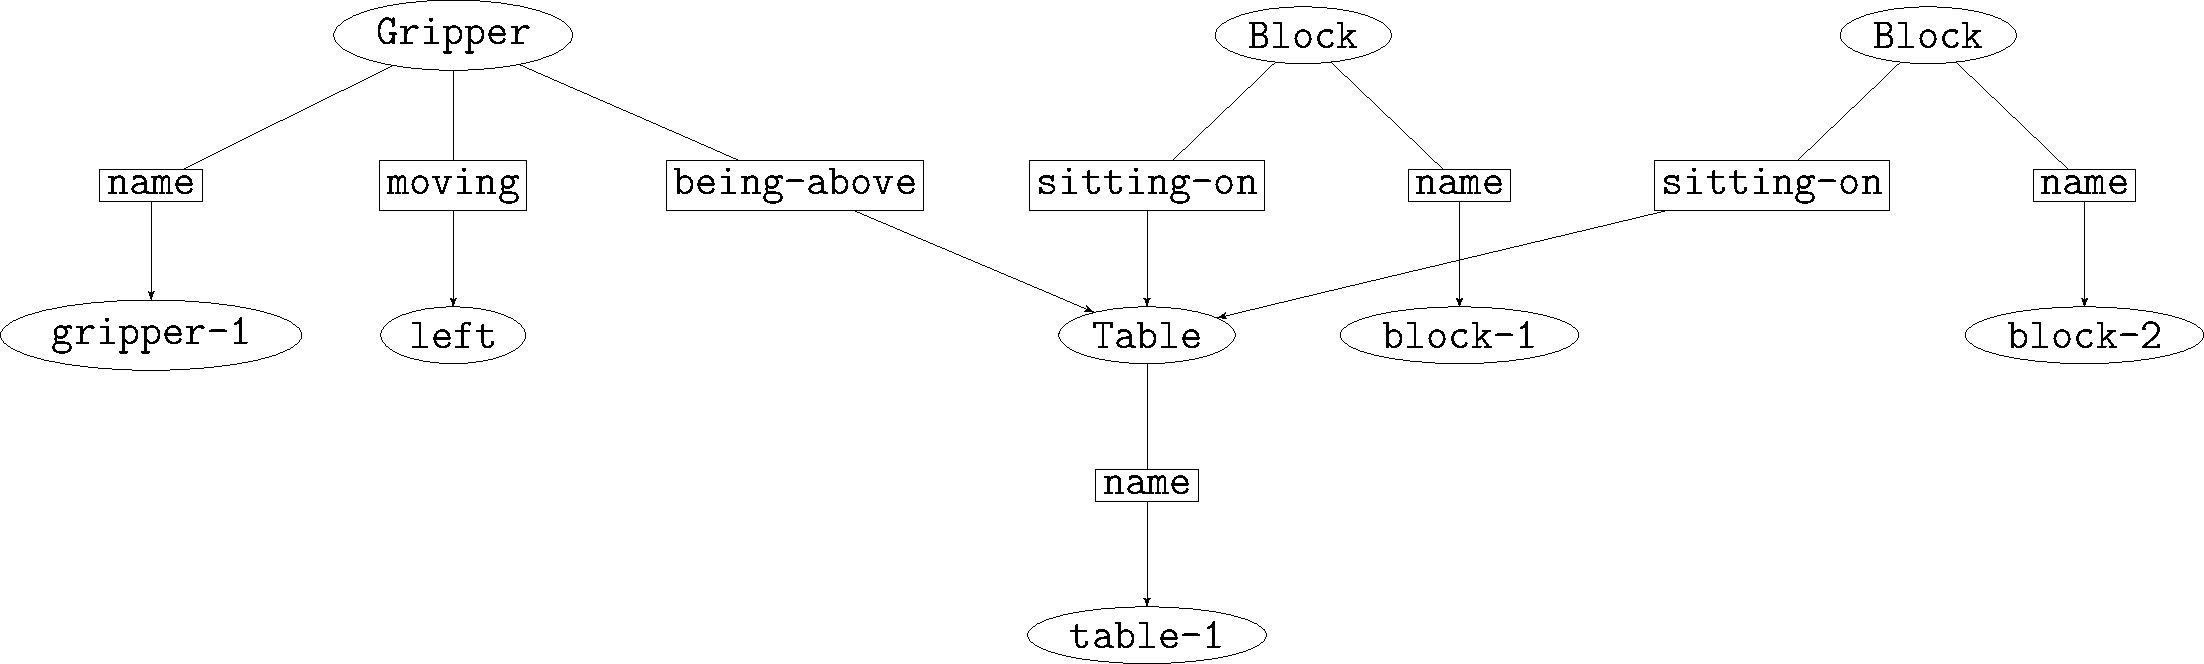
\includegraphics[width=12cm]{gfx/simulation_example_state}
\caption[A labelled graph representation of a state space.]{A labelled
  graph representation of a state space, where circles represent
  nodes, and squares represent edges.}
\label{figure:simulation_example_state}
\end{figure}

\section{Dot Notation for Graph-based Frame Objects}

Sometimes it is useful to refer to parts of a graph by considering
nodes in the graph to represent frame objects that have slotted
relationships with other frame objects.  Thus, I use a dot notation to
refer to the set of nodes that are connected to a given node, $v_1$,
through a given edge label, $\ell_e$, as defined in
{\mbox{\autoref{equation:frame_dot_notation}}}.
\begin{equation}
\label{equation:frame_dot_notation}
v_1.\ell_e = \{v_2 ~:~ (v_1, v_2) \in S_E \wedge \ell_e \in \nu[(v_1, v_2)]\}
\end{equation}

\section{Simulated Existence}

Activities in continuous Space actually exist.  Once we have
considered the activities in Duration to be the set of symbols, $S$,
we have assumed static representations for the actual dynamic.  The
dynamic does not have terms to help us in representing.  Therefore,
the question of existence becomes a question of whether or not a
symbol is in the set that is the current state of the simulation, $S$.
Equation~\ref{equation:define_exists} shows a definition of {\tt
  exists}, defined as the subgraph relationship between any state,
$G$, represented as a labelled graph, and the currently simulated
state graph, $S$:
\begin{equation}
\label{equation:define_exists}
\text{exists}(G) \longleftrightarrow G ~{\subseteq}~ S
\end{equation}




% Original definition of a graph as a 4-tuple with labelled nodes and edges

%\begin{definition}
%\label{definition:graph_first}
%\emph{
%A graph $G$ is the 4-tuple $(V, ~E, ~\nu, ~\nu)$, where
%\begin{itemize}
%\item $V$ is the set of vertices,
%\item $E ~{\subseteq}~ V ~{\times}~ V$ is the set of edges,
%\item $\nu : V \mapsto \ell_V$ is a function assigning a label to each vertex,
%\item $\nu : E \mapsto \{\ell_E\}$ is a function assigning a set of labels to each edge.
%\end{itemize}
%}\end{definition} \noindent In this definition, the edges are
%directed, i.e. there is an edge from $v_1$ to $v_2$ if $(v_1,
%v_2){\in}E$.  The empty graph, i.e. the graph with an empty set of
%vertices will be denoted by $\emptyset$.  The union of the sets of
%labels referred to by $\nu$ and $\nu$ will be sometimes be referred to
%with a dot notation, $\mathring{G}=\ell_V {\cup} \ell_E$.
%
%\begin{definition}
%\label{definition:graph_last}
%\emph{ Given a graph $G = (V, e, \nu, \nu)$, a \emph{subgraph} of $G$
%  is a graph $G_s = (V_s, e_s, \nu_s, \nu_s)$ such that
%\begin{enumerate}
%\item $V_s ~{\subseteq}~ V$
%\item $E_s ~{\subseteq}~ V_s {\times} V_s$,
%\item $\nu_s$ and $\nu_s$ are the restrictions of $\nu$ and $\nu$,
%  respectively, i.e.
%\begin{align*}
%\nu_s(v) &=         {\left\{
%                       \begin{array}{ll}
%                         \nu(v)           & \text{if }v {\in} V_s \\
%                         \text{undefined} & \text{otherwise}
%                       \end{array}
%                     \right.} \\
%\nu_s(e) &\subseteq {\left\{
%                       \begin{array}{ll}
%                        \nu(e)           & \text{if }e {\in} E_s \\
%                        \text{undefined} & \text{otherwise}
%                       \end{array}
%                     \right.}
%\end{align*}
%\end{enumerate}
%}\end{definition}



%\section{Simulating the Plan}
%


%\section{State Transitions (should be rewritten in simulation objects)} 

%\autoref{figure:blocks_world_gripper_over_block} shows an example of
%the next state of the simulation, $S[1]$.
%Equation~\ref{equation:example_next_state} gives an example
%description of the next state of the simulation model:
%\begin{figure}[bth]
%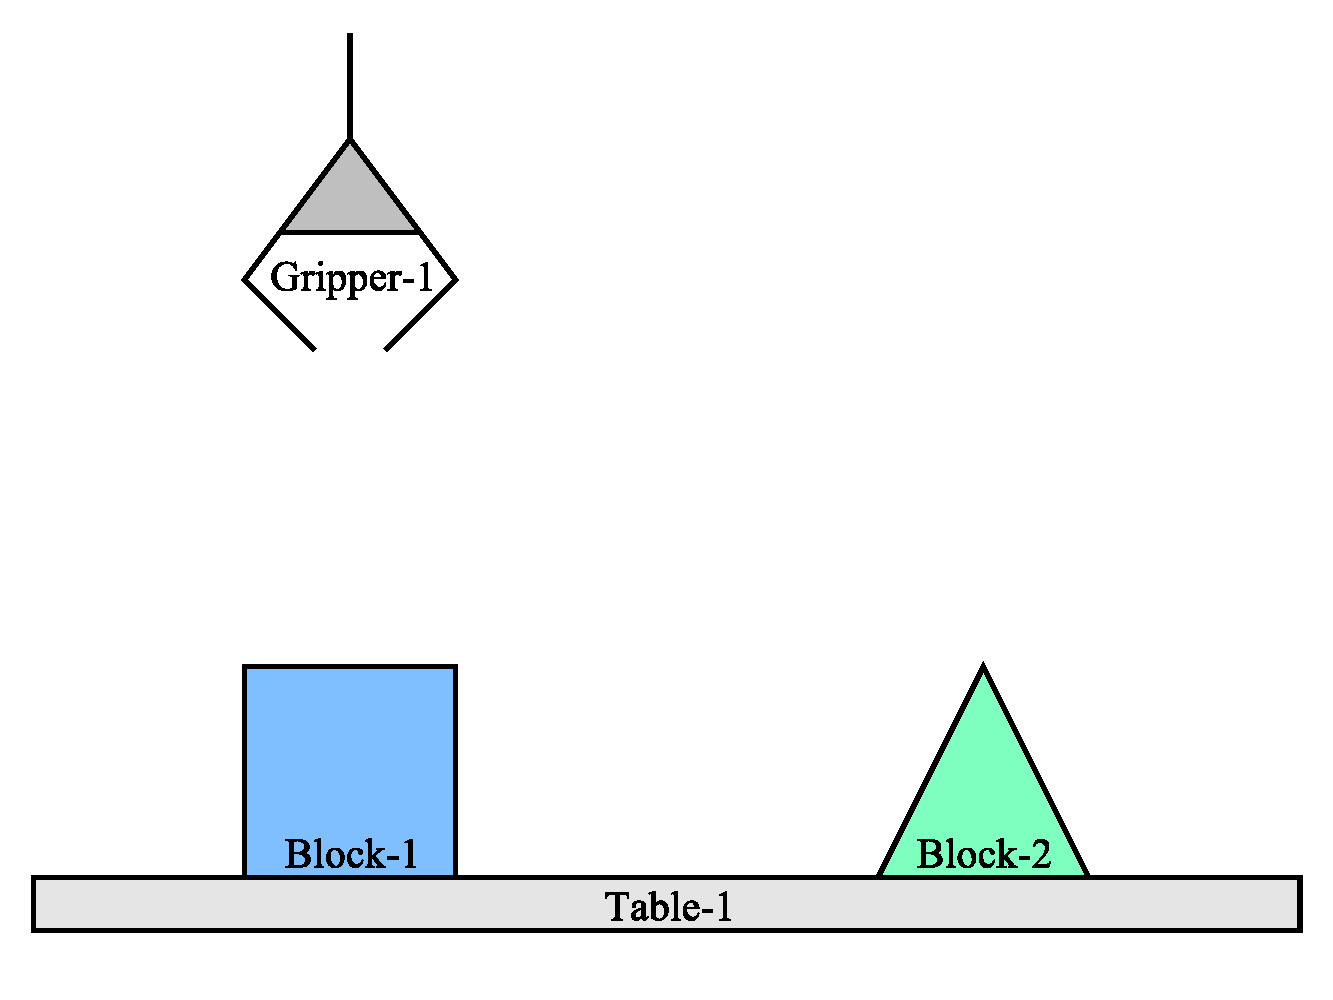
\includegraphics[width=10cm]{gfx/blocks_world_gripper_over_block}
%\caption{An example future state of simulation.}
%\label{figure:blocks_world_gripper_over_block}
%\end{figure}
%\begin{equation}
%\label{equation:example_next_state}
%S[1] =
%  \left\{
%    \begin{array}{l}
%      \text{{\tt Block-1-sitting-on-Table-1}}, \\
%      \text{{\tt Block-2-sitting-on-Table-1}}, \\
%      \text{{\tt Gripper-1-hovering-above-Table-1}}, \\
%      \text{{\tt Gripper-1-hovering-above-Block-1}}
%    \end{array}
%  \right\}
%\end{equation}
%
%Now, in order to begin to describe the activity of simulation, we must
%explicitly represent the transition, $T$, from one state to another.
%I refer to the resulting change to the state of the simulation as a
%\emph{state transition}.  The transition, $T[n]$, consists of two sets
%that keep track of changes, the \emph{add} set and the \emph{remove}
%set, as shown in Equation~\ref{equation:state_transition}:
%\begin{equation}
%\label{equation:state_transition}
%T[n] = \{T_\text{add}[n], ~T_\text{remove}[n]\}
%\end{equation}
%Equations~\ref{equation:predictive_state_transition}
%through~\ref{equation:transframe_last} give a definition of the
%transition, $T[n]$, in terms of the states, $S[n]$ and
%$S[n+1]$:
%\begin{align}
%\label{equation:predictive_state_transition}
%          S[n+1] & = S[n] ~{\cup}~ T_\text{add}[n] ~{\setminus}~ T_\text{remove}[n] \\
%         T_\text{remove}[n] & ~{\subseteq}~ S[n] \\
%         T_\text{remove}[n] & ~{\not\subseteq}~ S[n+1] \\
%            T_\text{add}[n] & ~{\subseteq}~ S[n+1] \\
%\label{equation:transframe_last}
%            T_\text{add}[n] & ~{\not\subseteq}~ S[n]
%\end{align}
%Equations~\ref{equation:state_transition_first}
%and~\ref{equation:state_transition_last} give the state transition,
%$T[n]$, for every step of the simulation:
%\begin{align}
%  \label{equation:state_transition_first}
%     T_\text{add}[n] &= S[n+1] ~{\setminus}~ S[n] \\
%  \label{equation:state_transition_last}
%  T_\text{remove}[n] &= S[n]   ~{\setminus}~ S[n+1]
%\end{align}
%Equation~\ref{equation:predictive_state_transition} shows the
%predictive potential for knowing the transition, $T[n]$, given the
%current state, $S[n]$.  Of course, $T[n]$ is defined in
%terms of $S[n]$ \emph{and} $S[n+1]$, so any
%predictive potential for
%Equation~\ref{equation:predictive_state_transition} is purely
%hypothetical.


%%************************************************
\chapter{Symbolic Representation}
\label{chapter:symbolic_representation}
%************************************************

\section{Representing Reflective Thinking Activity}

Reflective thinking exists as dynamic activities in Duration alongside
the physical activities that have just been described.  I will refer
to the subgraph of the simulation state, $S$, that represents the
$\text{reflective}^1$ thinking activities as $\mathcal{R}^1$.  The
first symbolic references to reflective thinking are now introduced to
this layer of the model.  Note that I have not introduced any specific
symbolic physical activity to the model.  The block example is just
that, an example.  Having the reflective focus be undescribed is
important because then the focus is not restricted, which allows a
recursive application of reflection to itself, whatever the specific
graph representation described.  This is a key point because the
general model of reflection applying to \emph{any} given labelled
graph means that it allows for this recursive definition of layered
reflective thinking.

\section{Physical Activity is Any Prior Existing Graph}

The graph of physical activities must necessarily exist prior to
reflectively thinking about it.  Because this prior activity is
defined to be \emph{any} graph, what remains in order to build $n$
layers of reflective thinking activity is to define planning activity
that reflects upon this prior activity.  Therefore, subsequently, no
matter what the reflective thinking description, this reflective
thinking activity can be duplicated in $n$ reflective layers that will
think about any given graph representation of activity.  Allowing the
physical activity to a be an undescribed graph is important in order
to allow this recursion.  Notice that the physical activity is not
necessarily composed of anything resembling objects, since graphs are
a general representation that could just as easily represent one
single number line, or even an infinitely finely interpolated
multidimensional Space.  If some prior physical activity can be
represented as a graph, then this simulation of reflective thinking is
applicable.

\section{Defining N Layers of Reflective Thinking Activities}

Layers of reflective activity are defined inductively, beginning with
$\text{reflective}^0$ layer of activity, $\mathcal{R}^0$, as the
initial given physical activity.  Then, each subsequent layer of
$\text{reflective}^{n+1}$ thinking activity, $\mathcal{R}^{n+1}$, is
defined in terms of $\mathcal{R}^n$ in
{\mbox{Equations~\ref{equation:define_reflective_n_activity_graph_first}}}
{\mbox{through~\ref{equation:define_reflective_n_activity_graph_last}}}.
\begin{align}
\label{equation:define_reflective_n_activity_graph_first}
                                        \mathcal{R}^0 &\equiv \text{\emph{Physical Layer of Activities}} \\
                                   \mathcal{R}^{n+1}_V &\subset S_V \setminus \bigcup_{k=0}^n\mathcal{R}^k_V \\
                                   \mathcal{R}^{n+1}_E &= (\mathcal{R}^{n+1}_V \times \mathcal{R}^{n+1}_V) \cap S_E \\
                              \mathcal{R}^{n+1}_\mu(v) &= {\left\{
                                                            \begin{array}{ll}
                                                              S_\mu(v)         & \text{if }v {\in} \mathcal{R}^{n+1}_V \\
                                                              \text{undefined} & \text{otherwise}
                                                            \end{array}
                                                          \right.} \\
\label{equation:define_reflective_n_activity_graph_last}
                              \mathcal{R}^{n+1}_\nu(e) &= {\left\{
                                                            \begin{array}{ll}
                                                              S_\nu(e)          & \text{if }e {\in} \mathcal{R}^{n+1}_E \\
                                                              \text{undefined} & \text{otherwise}
                                                            \end{array}
                                                          \right.}
\end{align}
Note that there can be edges between activities in subsequent layers.
These edges are not within any of the graphs of the reflective layers
of thinking, but they do exist in the state graph, $S$.  The edges
that relate the reflective layers of activity in the simulation model
are a necessary component of dynamic symbolic references to activities
in the layers below the symbolic activity.  In other words,
$\bigcup_{k=0}^\infty\mathcal{R}^k\ \subset\ S$, the simulation state
is greater than the union of its reflective layers.

\section{Representing Static Symbols}

In order to describe symbolization, a representation for a simulated
symbol must be defined.  A symbol is the most interesting object in
the model because it functions as a static reference to the dynamic,
while being fundamentally dynamic itself.  There are two primary
features of a symbolic reference:
\begin{itemize}
\item A symbol functions as a static reference and, thus, can be
  ordered in Spatial arrangements that function as static orderings.
\item A symbol is fundamentally dynamic and, thus, exists as dynamic
  activities in a referential dynamic continuous Spatial relationship
  with other dynamic activities in Duration.
\end{itemize}
A symbol is actively maintained in Duration, so the existence of a
simulated symbol in the simulation model would need to be added to the
set of all simulated activities in Duration.  The set of symbols* in
layer $n$ is defined to be $X^{n*}$.
{\mbox{Equations~\ref{equation:define_symbol_first}}}
{\mbox{and~\ref{equation:define_symbol_last}}} define layered sets of
symbols*:
\begin{align}
\label{equation:define_symbol_first}
           X^{n*} &= \left\{x^* : \begin{array}{l}
                                   x^* \in \mathcal{R}^n_V ~\wedge~ \\
                                   ~~\left(\forall_{v \in \mathcal{R}^n_V}, \begin{array}{l}
                                                                          S_\mu(v) = \text{\tt{Reflective}} \rightarrow \\
                                                                          ~~x^* \in v.\text{\tt{symbol}}
                                                                        \end{array}\right)
                                 \end{array}\right\} \\
\label{equation:define_symbol_last}
           x^{n*} &\in X^{n*}
\end{align}

\section{Representing Symbolic Reference}

Because dynamic activities in Duration cannot be ordered in Space by
the reflective thinking layers, the most important aspect of the
reflective simulation is the capability to create a static reference,
$x^*$, which has an associated dynamic representation of an arbitrary
subgraph of activity, $\Psi(x^*)$.  Note that while $\Psi(x^*)$
represents a potential subgraph of the simulation state, this subgraph
may or may not actually exist in the simulation state, $S$.  This
symbolic representative capability is the basis of symbolic perception
and memory.

Because the simulation state is a static symbolic representation of
the actual dynamic activities in Duration, simulation of the dynamic
reflective representation must also be in the same simulated terms of
dynamic physical activities.  Considering this dynamic activity to be
symbolic helps in explaining the relationship between the dynamic and
the static, as long as the distinction is kept clear and the
simulation of the dynamic is not confused with the simulation of the
static.  The confusion would arise because both are modelled as
symbols in the state graph, $S$, of the simulation model.  Of course,
in actuality, the dynamic physical activities do not have symbolic
terms.  I will continue to use the asterisk (*) notation when
referring to the simulation of actively static symbolic references as
opposed to the simulation of the otherwise purely dynamic activities
in Duration.
{\mbox{Equations~\ref{equation:first_order_reflection_representation_in_state_first}}}
{\mbox{through~\ref{equation:first_order_reflection_representation_in_state_last}}}
show a definition of a static symbolic reference, $x^*$, to a dynamic
reflective representation of a subgraph of activity, $\Psi(x^*)$, not
necessarily actually within the state graph, $S$.
\begin{align}
\label{equation:first_order_reflection_representation_in_state_first}
                                                   \forall_{v \in \Psi_V(x^*)}, ~v &\in x^*.\text{\tt{node}} \\
                                 \forall_{v \in \Psi_V(x^*)}, ~v.\text{\tt{label}} &= \{\Psi_\mu(x^*)(v)\} \\
                                                   \forall_{e \in \Psi_E(x^*)}, ~e &\in x^*.\text{\tt{edge}} \\
     \forall_{e \in \Psi_E(x^*)}, ~[e = (e_{v_1}, e_{v_2}) \wedge e.\text{\tt{tail}} &= \{e_{v_1}\}] \\
     \forall_{e \in \Psi_E(x^*)}, ~[e = (e_{v_1}, e_{v_2}) \wedge e.\text{\tt{head}} &= \{e_{v_2}\}] \\
\label{equation:first_order_reflection_representation_in_state_last}
                                 \forall_{e \in \Psi_E(x^*)}, ~e.\text{\tt{label}} &= \{\Psi_\nu(x^*)(e)\}
\end{align}
{\mbox{\autoref{figure:simulation_reflective_1_example_state}}} shows
an example of the representation for a symbolic reference to the
$\text{reflective}^0$ layer in the $\text{reflective}^1$ layer.
\begin{figure}
\center
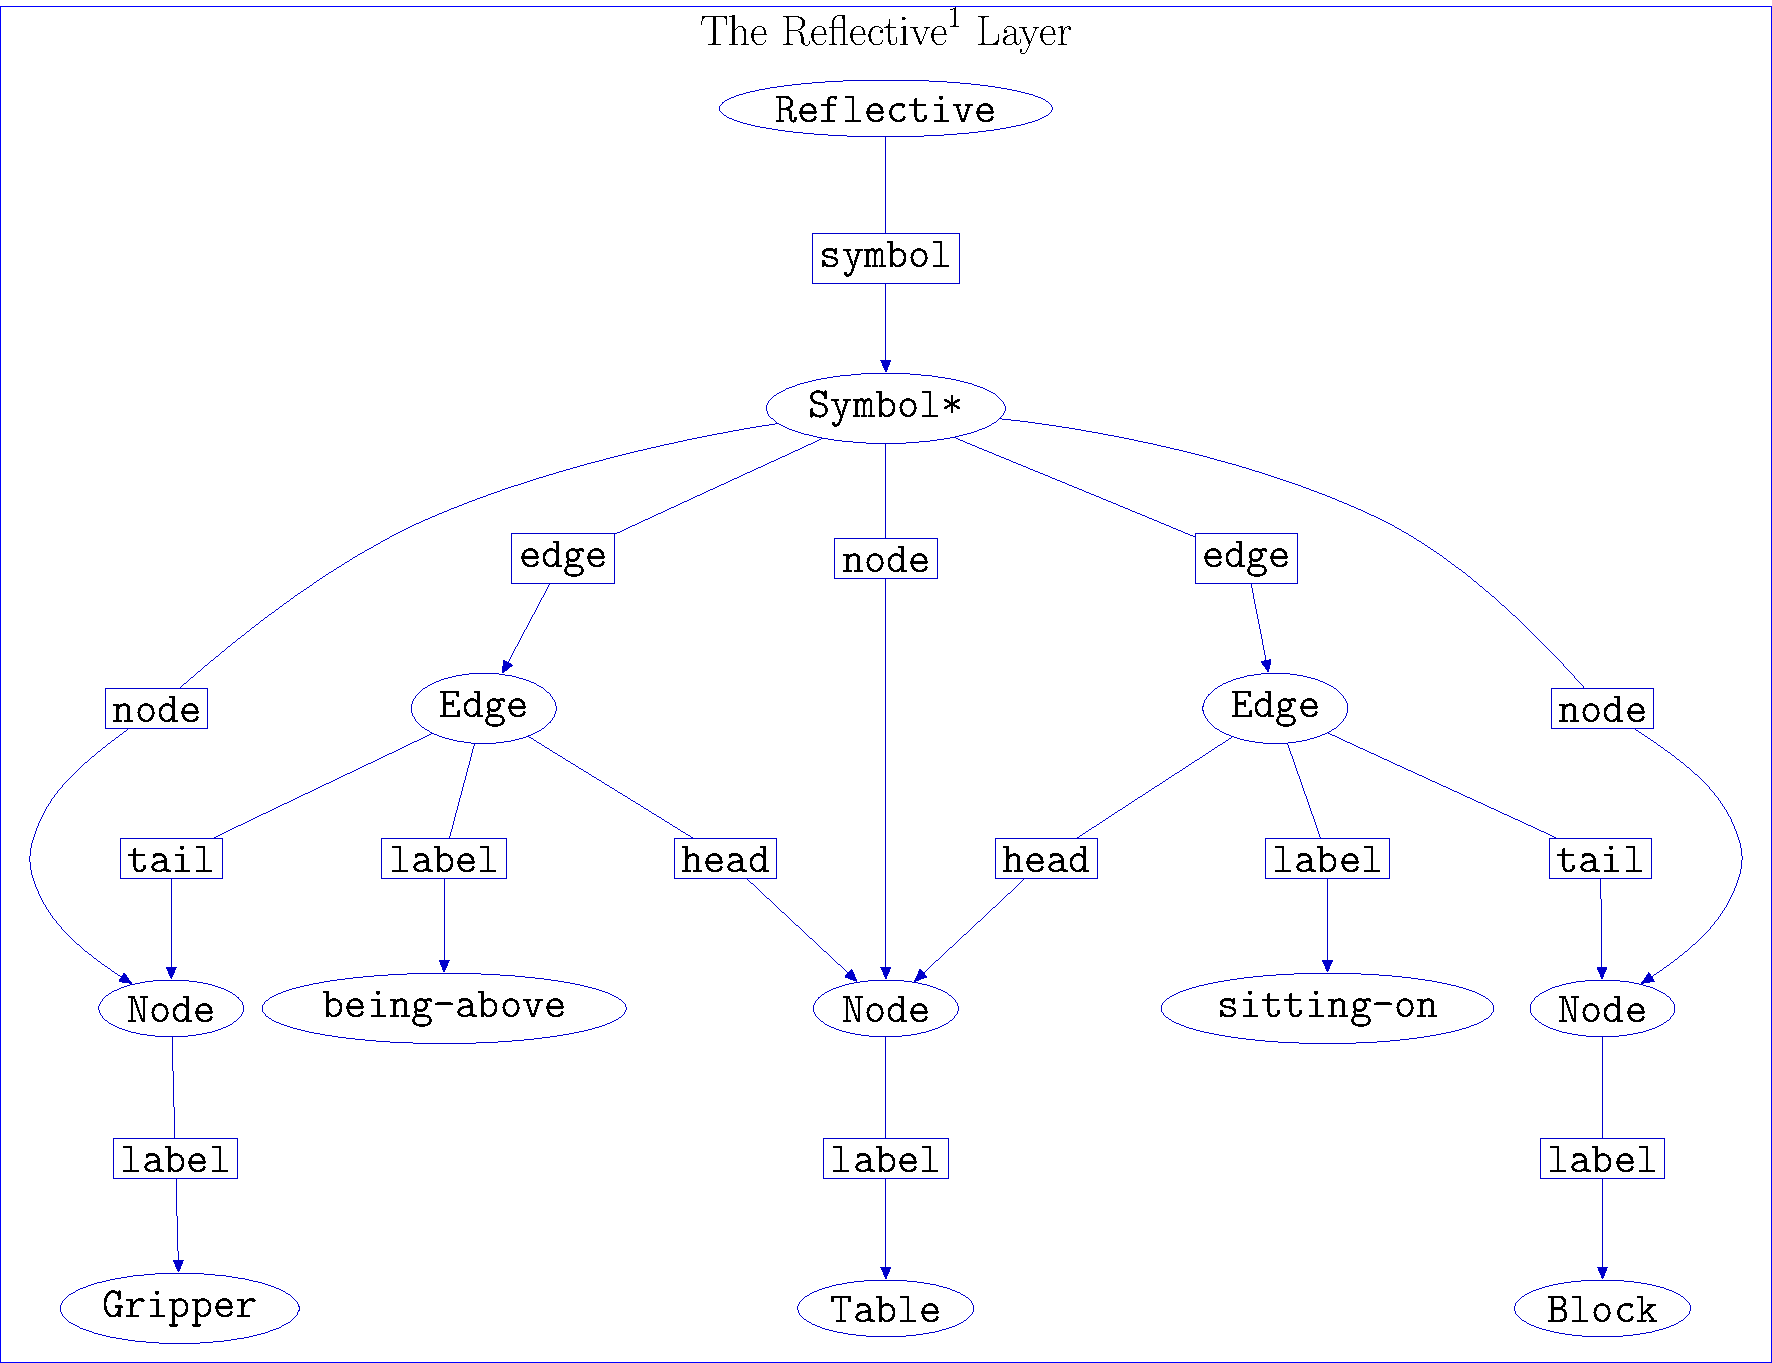
\includegraphics[width=12cm]{gfx/simulation_reflective_1_example_state}
\caption[An example of the representation for symbolic reference.]{An
  example of the representation for symbolic reference, where the
  dynamic referent is the physical activity of a block being on a
  table in conjunction with a gripper being above the same table.}
\label{figure:simulation_reflective_1_example_state}
\end{figure}

\section{A Visualization of a Reflective Relationship}

When reflective graph structures, as in
{\mbox{\autoref{figure:simulation_reflective_1_example_state}}}, get
to be larger, they can be confusing when shown in full structural
detail.  In order to simplify the visual representation of a
reflective relationship, I will sometimes use a trapezoidal edge-like
visual in order to present the same complicated relationship structure
in a simpler way.
{\mbox{\autoref{figure:reflective_relationship_visualization}}} shows
a simpler visualization of the same example reflective relationship.
\begin{figure}
\center
\includegraphics[width=6cm]{gfx/reflective_relationship_visualization}
\caption[A shorthand visualization for a symbolic reference.]{A
  shorthand visualization for a symbolic reference, where the
  trapezoid is a shorthand, for the same representation depicted in
  {\mbox{\autoref{figure:simulation_reflective_1_example_state}}}.
  The symbolic referent subgraph is pictured in red because this
  subgraph does not actually exist in the simulation state graph, $S$.
  Instead, the symbolic referent subgraph's \emph{representation}
  actually dynamically exists in the simulation state graph,
  $S$. Thus, the symbolic representation operator, $\Psi$, is not a
  symbol in the state graph, $S$, but represents the relationship to
  the representation of the non-existent subgraph that appears in
  red.}
\label{figure:reflective_relationship_visualization}
\end{figure}

\section{Representing Symbolic Perception and Memory}

{\mbox{\autoref{figure:example_symbolic_reference_to_physical_activity}}}
shows an example of a symbol*, $x^*$, in the first-order reflective
layer.  Notice that $\Psi(x^*)$ is isomorphic to a subgraph of the
$\text{reflective}^0$ layer, $\mathcal{R}^0$.  When a symbolic
representation is isomorphic to a subgraph of the layers below it, the
symbol is said to be a {\emph{symbolic perception}}, or simply, a
{\emph{percept}}.
{\mbox{\autoref{equation:definition_of_symbolic_percept}}} defines
when a symbolic referent is considered a percept based on its
isomorphic relationship with layers of activity below it:
\begin{equation}
\label{equation:definition_of_symbolic_percept}
\text{percept}^n(x^*) = \left\{\begin{array}{ll}
                                 \begin{array}{l}
                                   \text{\emph{True}} \\
                                   \text{~~}
                                 \end{array} & \begin{array}{l}
                                                 \text{if } \Psi(x^*) \text{ is isomorphic to a} \\
                                                 \text{~~subgraph of } S \setminus \bigcup_{k=n}^\infty{\mathcal{R}^k}
                                               \end{array} \\
                                 \begin{array}{l}
                                   \text{\emph{False}}
                                 \end{array} & \text{otherwise}
                               \end{array}\right.
\end{equation}
{\mbox{\autoref{figure:example_symbolic_memory}}} shows a symbolic
reflective reference to the physical layer of activity that is not
perceived because it is not isomorphic to any subgraph in the
$\text{reflective}^0$ layer, $\mathcal{R}^0$.  When a symbol is not
isomorphic to a subgraph in the layers below it, this is referred to
as a \emph{symbolic memory}.
\begin{figure}
\center
\includegraphics[height=8cm]{gfx/example_symbolic_reference_to_physical_activity}
\caption[Example of a perceived first-order symbolic reference to the
  physical layer of activity.]{Example of a perceived first-order
  symbolic reference to the physical layer of activity,
  i.e. $\Psi(x^*)$ is isomorphic to a subgraph of $\mathcal{R}^0$.}
\label{figure:example_symbolic_reference_to_physical_activity}
\end{figure}
\begin{figure}
\center
\includegraphics[height=8cm]{gfx/example_symbolic_memory}
\caption[Example of a non-perceived symbol, or symbolic
  memory.]{Example of a non-perceived symbol, or symbolic memory,
  $x^*$, i.e. $\Psi(x^*)$ is not isomorphic to a subgraph of
  $\mathcal{R}^0$.}
\label{figure:example_symbolic_memory}
\end{figure}

\section{Second-order Symbolic Representation}

The second-order layer of reflective thinking is the first layer that
can reflect on the existence of the symbols of the first-order
reflective layer.
{\mbox{\autoref{figure:example_second_order_symbol}}} shows an example
of a second-order symbolic reference to a first-order symbolic
representation.
\begin{figure}
\center
\includegraphics[width=12cm]{gfx/example_second_order_symbol}
\caption[Example of a second-order symbol representing first-order
  symbolization activity.]{Example of a second-order symbol
  representing an aspect of first-order symbolization.  Note that the
  actually existent symbolic representation in the first-order
  reflective layer is shown in full detail, while the red subgraph in
  the second-order symbolic representation is short-hand for the much
  more complex actually existent activity in this layer.}
\label{figure:example_second_order_symbol}
\end{figure}

\section{Representing Symbolic Resources}

Each reflective thinking layer in the model has a set of built-in
resources.  These built-in resources correspond to what
\cite{minsky:2006} refers to as the built-in reactive resources.
Resources can be in activated or suppressed Spatial arrangements.
These activated and suppressed relationships can lead to logical
conflicts, a type of activation failure.

Because the simulation is of actual dynamic reflective thinking and
not of a simulation of an already symbolic control system, how to
think about resources in my system appears as something like a
cooperation between the physical layer and the first-order reflective
resources.  The set of resources, $A^{n*}$, is a subset of the
symbols, $X^{n*}$, in any given layer.  They are symbolic references
to the lower layers of continuous dynamic activity.
{\mbox{\autoref{figure:example_resource}}} shows an example of a
first-order reflective resource, a symbolic reference to the
$\text{reflective}^0$ layer of dynamic physical activity.
{\mbox{Equation~\ref{equation:define_resource_set_first}}}
{\mbox{through~\ref{equation:define_resource_set_last}}} define a
symbolic $\text{resource}^*$, $a^{n*}$, in the simulation state graph,
$S$.
\begin{align}
\label{equation:define_resource_set_first}
                                       A^{n*} &\equiv \text{\emph{$\text{Reflective}^n$ action resources.}} \\
                                       A^{n*} &\subseteq X^{n*} \\
\text{\tt{reflective}}^n.\text{\tt{resource}} &= A^{n*} \\
\label{equation:define_resource_set_last}
                                       a^{n*} &\in A^{n*}
\end{align}
{\mbox{\autoref{figure:example_resource_conflict}}} shows an example
of four resources, each displaying a different activation or
suppression Spatial relationship:
\begin{enumerate}
\item An example of an activation relationship.
\item An example of a suppression relationship.
\item An example of an idle resource in neither an activation nor a
  suppression relationship.
\item An example of a resource in simultaneous, conflicting,
  activation and suppression relationships.
\end{enumerate}
\begin{figure}
\center
\includegraphics[width=12cm]{gfx/example_resource}
\caption[An example of a first-order reflective resource.]{An example
  of a first-order reflective resource that refers to the dynamic
  activity in the $\text{reflective}^0$ layer of physical activity.}
\label{figure:example_resource}
\end{figure}
\begin{figure}
\center
\includegraphics[width=12cm]{gfx/example_resource_conflict}
\caption[Four examples of resource activation and suppression Spatial
  relationships.]{Four examples of resource activation and suppression
  Spatial relationships: (1) activation, (2) suppression, (3) idle,
  and (4) conflict.  Note that all of these activation and suppression
  events have the same starting simultaneity and no ending.  In
  general, activation and suppression events may be historical
  memories, and do not necessarily imply present activation,
  suppression, or conflict.}
\label{figure:example_resource_conflict}
\end{figure}


%%************************************************
\chapter{Grounded Factual Knowledge}
\label{chapter:grounded_factual_knowledge}
%************************************************

Spatial arrangements of static symbols are created by the reflective
thinking layers.  Static symbols are not contained within the physical
layer, but these symbols are used to represent ongoing causal
transitions from the past to the future.  These grounded
representations form the basis from which causal hypotheses can be
abstracted.  Hypothetical causal models enable planning activities to
imagine counterfactual knowledge of the past and future.  Second-order
dynamically grounded causal transitions that factually describe this
first-order planning activity allows the abstraction of second-order
hypothetical causal knowledge that allows the creation of
counterfactual knowledge about the hypothetical necessities and
results of planning activities themselves.

This chapter will discuss how grounded knowledge representations form
the basis of hypothetical abstractions of both physical activities as
well as reflective thinking activities.  Having a dynamically grounded
reference for factual knowledge about every layer of reflective
thinking is necessary for debugging hypothetical counterfactual
conclusions in any layer when these conclusions turn out to be wrong.
Keeping clear distinctions between dynamically grounded factual
knowledge and the subsequent practically motivated hypothetical
derivations, gives a clear way to think about facts that are known to
be true, while the symbolic basis for this grounded factual knowledge
can be reflectively refined when the utility of hypothetical
derivative assumptions end up failing to be useful.

Thus, I must first describe the $N$ layers of dynamically grounded
factual causal transitions that are the basis for the hypothetical and
counterfactual derivations used for the $N$ layers of planning.
Clearly understanding the derivation of $N$ layers of planning
knowledge leads naturally to a simple debugging method for $N$
reflective layers of knowledge maintenance, the focus of this thesis.

\section{Simultaneities}

Simultaneities form the simplest component of the representational
machinery of present grounded factual knowledge in the simulation
model.  Using the notation of the previous chapter, the set of
currently perceived symbols, $\mathcal{P}^{n*}$, and the set of
unperceived symbols, $\overline{\mathcal{P}}^{n*}$, in the
$n^{\text{th}}$-order reflective thinking layer are defined in
{\mbox{Equations~\ref{equation:define_first_order_perceived_symbols}}}
{\mbox{and~\ref{equation:define_first_order_unperceived_symbols}}}.
\begin{align}
\label{equation:define_first_order_perceived_symbols}
           \mathcal{P}^{n*} &= \{x^* : x^* \in X^{n*} \wedge \text{percept}^n(x^*)\} \\
\label{equation:define_first_order_unperceived_symbols}
\overline{\mathcal{P}}^{n*} &= \{x^* : x^* \in X^{n*} \wedge \neg\text{percept}^n(x^*)\}
\end{align}
{\mbox{Equation~\ref{equation:define_reflective_n_present_simultaneity}}}
defines the graph representation that exists in the simulation state,
$S$, of the present grounded factual simultaneity for each
$\text{reflective}^n$ layer of thinking activity.
\begin{equation}
\label{equation:define_reflective_n_present_simultaneity}
\begin{array}{l}
 (t \in \text{\tt{reflective}}^n.\text{\tt{present}}) \longrightarrow \\
\begin{array}{l}
\text{\makebox[4cm][r]{    $(t.\text{\tt{percept}}$}}= \mathcal{P}^{n*}) ~\wedge~ \\
\text{\makebox[4cm][r]{$(t.\text{\tt{not-percept}}$}}= \overline{\mathcal{P}}^{n*})
\end{array}
\end{array}
\end{equation}
{\mbox{\autoref{figure:example_simultaneity}}} shows a simple example
of a present grounded factual simultaneity in the first-order
reflective thinking layer.
\begin{figure}
\center
\includegraphics[width=10cm]{gfx/example_simultaneity}
\caption[Example simultaneity of positive and negative symbolic
  perceptions.]{Example simultaneity of positive and negative symbolic
  perceptions, where the symbolic reference to the dynamic physical
  activity of a block sitting on a table is perceived, while a block
  sitting on another block is not.}
\label{figure:example_simultaneity}
\end{figure}

\section{Transitions}

Simultaneities can be ordered in temporal relationships in each
reflective layer.
{\mbox{Equation~\ref{equation:define_reflective_n_time}}} defines the
graph representation in the simulation state, $S$, that keeps track of
the grounded knowledge of all temporal orderings of previous
perceptual simultaneities.
\begin{equation}
\label{equation:define_reflective_n_time}
\text{\tt{reflective}}^n.\text{\tt{time}} \equiv \text{\emph{Transitions of the $\text{Reflective}^n$ Layer}}
\end{equation}
Given this representation of temporal orderings for each
$\text{reflective}^n$ layer,
{\mbox{Equations~\ref{equation:reflective_n_temporal_ordering_first}}}
{\mbox{and~\ref{equation:reflective_n_temporal_ordering_last}}} define
the transitive temporal relationship, $\stackrel{n}{<}$, that
describes a separate ordering of grounded simultaneities for each
reflective layer.
\begin{align}
\label{equation:reflective_n_temporal_ordering_first}
\left(\begin{array}{l}
  x^* \in \text{\tt{reflective}}^n.\text{\tt{time}} ~\wedge~ \\
  ~~t_1 \in x^*.\text{\tt{past}} ~\wedge~ t_2 \in x^*.\text{\tt{future}}
\end{array}\right) &\longrightarrow t_1 \stackrel{n}{<} t_2 \\
\label{equation:reflective_n_temporal_ordering_last}
(t_1 \stackrel{n}{<} t_2 ~\wedge~ t_2 \stackrel{n}{<} t_3) &\longrightarrow t_1 \stackrel{n}{<} t_3
\end{align}
{\mbox{Equation~\ref{equation:reflective_n_temporally_ordered_set}}}
defines the separate set of ordered simultaneities within each
$\text{reflective}^n$ layer.
\begin{equation}
\label{equation:reflective_n_temporally_ordered_set}
 T^n = \left\{t : 
\begin{array}{l}
  x^* \in \text{\tt{reflective}}^n.\text{\tt{time}} ~\wedge~ \\
  ~~(t \in x^*.\text{\tt{past}} ~\vee~ t \in x^*.\text{\tt{future}})
\end{array}\right\}
\end{equation}
{\mbox{Equation~\ref{equation:define_time_connected_full_ordering}}}
defines each set of temporally ordered simultaneities, $T^n$, is a
connected and fully ordered sequence.
\begin{equation}
\label{equation:define_time_connected_full_ordering}
(t_1 \in T^n \wedge t_2 \in T^n) \longrightarrow (t_1 \stackrel{n}{<} t_2 \vee t_2 \stackrel{n}{<} t_1 \vee t_1 = t_2)
\end{equation}
{\mbox{\autoref{figure:example_transition}}} shows an example of how
three simultaneities can be represented in a simulation state graph as
temporally ordered using two transition relationships.
\begin{figure}
\center
\includegraphics[width=14cm]{gfx/example_transition}
\caption[An example of two transitions ordering three
  simultaneities.]{An example of two transitions ordering three
  simultaneities: (1) a block sitting on a table, (2) a block not
  sitting on a table, and (3) a block sitting on another block.}
\label{figure:example_transition}
\end{figure}

\section{Perceptual Events}

{\mbox{Equation~\ref{equation:define_perceived}}} defines a
``perceived'' Spatial relationship for each reflective layer that can
exist between a temporal simultaneity, $t$, and a static symbolic
reference, $x^*$, to the layers below.
\begin{equation}
\label{equation:define_perceived}
\text{perceived}^n(t, x^*) = (t \in T^n ~\wedge~ x^* \in t.\text{\tt{percept}})
\end{equation}
{\mbox{Equation~\ref{equation:define_event_start}}} defines the start
times for perceptual events in each reflective layer.  A perceptual
event begins at the time when a symbol is perceived and has just
immediately transitioned from not being perceived.
\begin{equation}
\label{equation:define_event_start}
\begin{array}{l}
  \text{start}^n(t, x^*) = \\
  ~~\left(
  \begin{array}{l}
  \text{perceived}^n(t, x^*) ~\wedge~ \\
  ~~\left[
  \begin{array}{l}
  \forall_{t_1 \in T^n}, \\
  ~~\left(\begin{array}{l}
            \left[\begin{array}{l}
                    t_1 \stackrel{n}{<} t ~\wedge~ \\
                    ~~\text{perceived}^n(t_1, x^*)\end{array}\right] \longrightarrow \\
            ~~\exists_{t_2 \in T^n}, \\
            ~~~~\left[\begin{array}{l}
                        t_1 \stackrel{n}{<} t_2 \stackrel{n}{<} t ~\wedge~ \\
                        ~~\neg\text{perceived}^n(t_2, x^*)\end{array}\right]\end{array}\right)
  \end{array}
  \right]
  \end{array}\right)
\end{array}
\end{equation}
{\mbox{Equation~\ref{equation:define_event_end}}} defines the end
times for perceptual events in each reflective layer.  A perceptual
event ends at the time when a symbol is perceived and will immediately
transition to not being perceived at the subsequent time.
\begin{equation}
\label{equation:define_event_end}
\begin{array}{l}
  \text{end}^n(t, x^*) = \\
  ~~\left(
  \begin{array}{l}
  \text{perceived}^n(t, x^*) ~\wedge~ \\
  ~~\left[
  \begin{array}{l}
  \forall_{t_1 \in T^n}, \\
  ~~\left(\begin{array}{l}
            \left[\begin{array}{l}
                    t \stackrel{n}{<} t_1 ~\wedge~ \\
                    ~~\text{perceived}^n(t_1, x^*)\end{array}\right] \longrightarrow \\
            ~~\exists_{t_2 \in T^n}, \\
            ~~~~\left[\begin{array}{l}
                        t \stackrel{n}{<} t_2 \stackrel{n}{<} t_1 ~\wedge~ \\
                        ~~\neg\text{perceived}^n(t_2, x^*)\end{array}\right]\end{array}\right)
  \end{array}
  \right]
  \end{array}\right)
\end{array}
\end{equation}
Between the start and end times of a perceptual event, a symbol has
been continuously perceived.  Event knowledge is factual knowledge
that is grounded in the perception of the dynamic.  Factual knowledge
does not involve hypothetical reasoning.  Later, I will show how
hypothetical assumptions can be abstracted from factual event
knowledge.  Grounded factual knowledge is the source of all
hypothetical abstractions that are used in planning.  Thus, grounded
knowledge is the necessary foundation for creating a planning
algorithm that can be debugged when the hypothetical bases of
counterfactual knowledge turn out to be contradicted by further
factual knowledge.
{\mbox{Equations~\ref{equation:define_perceptual_event_first}}}
{\mbox{through~\ref{equation:define_perceptual_event_last}}} define a
perceptual event in the $n^{\text{th}}$-order reflective layer.
\begin{align}
\label{equation:define_perceptual_event_first}
                                         e &\in \text{\tt{reflective}}^n.\text{\tt{event}} \\
                      e.\text{\tt{symbol}} &= \{x^*\} \\
                       e.\text{\tt{start}} &= \{t_\text{start}\} \\
                         e.\text{\tt{end}} &= \{t_\text{end}\} \\
                             t_\text{start} &\in \{t : t \in T^n \wedge \text{start}^n(t, x^*)\} \\
                               t_\text{end} &\in \{t : t \in T^n \wedge \text{end}^n(t, x^*)\} \\
                             t_\text{start} &\stackrel{n}{<} t_\text{end} \\
\label{equation:define_perceptual_event_last}
 \neg\exists_{t \in T^n}, [t_\text{start} &\stackrel{n}{<} t \stackrel{n}{<} t_\text{end} \wedge \text{end}^n(t, x^*)]
\end{align}

\section{Event Transframes}

While transitions represent a temporal relationship between two
simultaneities, a \emph{transframe} represents the difference between
two simultaneities.  For example, two simultaneities could both
contain a lot of perceptual information, but the transframe between
them might be a very small set of differences.  The difference between
two simultaneities is kept track of as two lists: (1) the additions
and (2) the removals from the actively perceived symbols in each
simultaneity.  {\mbox{\autoref{figure:example_transframe}}} shows an
example of a perceptual event that has an associated transframe.
\begin{figure}
\center
\includegraphics[width=12cm]{gfx/example_transframe}
\caption[An example of a factual event transframe.]{An example of a
  factual event transframe, representing the continuous perception of
  the symbol that refers to the dynamic physical activity of a gripper
  being above a block.  The symbolized perceptual difference between
  the starting and ending simultaneities is represented by a
  transframe of the perceptual event, listing the symbolic additions
  and removals from the starting and ending situations.  Note that
  negative perceptions in both the simultaneities and the transframe
  have been omitted for clarity.}
\label{figure:example_transframe}
\end{figure}

\section{Resources}

Each reflective thinking layer in the model has a set of built-in
resources.  These built-in resources correspond to what
\cite{minsky:2006} refers to as the built-in reactive resources.
Resources can be in activated or suppressed Spatial arrangements.
These activated and suppressed relationships can lead to logical
conflicts, which can be debugged by tracing the causal dependencies of
the creation of these Spatial arrangements.  Before discussing these
causal dependencies, the learned hypothetical knowledge that is used
for creating the plans whose execution creates these Spatial
arrangements must first be described.
{\mbox{Equation~\ref{equation:define_resource_set_first}}}
{\mbox{through~\ref{equation:define_resource_set_last}}} defines the
action resources in each $\text{reflective}^n$ layer.
\begin{align}
\label{equation:define_resource_set_first}
                                       A^{n*} &\equiv \text{\emph{$\text{Reflective}^n$ action resources.}} \\
\text{\tt{reflective}}^n.\text{\tt{resource}} &= A^{n*} \\
\label{equation:define_resource_set_last}
                                       a^{n*} &\in A^{n*}
\end{align}
{\mbox{\autoref{figure:example_resource}}} shows an example of a
first-order reflective resource, a symbolic reference to the
$\text{reflective}^0$ layer of dynamic physical activity.
{\mbox{\autoref{figure:example_resource_conflict}}} shows an example
of four resources, each displaying a different activation or
suppression Spatial relationship:
\begin{enumerate}
\item An example of an activation relationship.
\item An example of a suppression relationship.
\item An example of an idle resource in neither an activation nor a
  suppression relationship.
\item An example of a resource in simultaneous, conflicting,
  activation and suppression relationships.
\end{enumerate}
\begin{figure}
\center
\includegraphics[width=12cm]{gfx/example_resource}
\caption[An example of a first-order reflective resource.]{An example
  of a first-order reflective resource that refers to the dynamic
  activity in the $\text{reflective}^0$ layer of physical activity.}
\label{figure:example_resource}
\end{figure}
\begin{figure}
\center
\includegraphics[width=12cm]{gfx/example_resource_conflict}
\caption[Four examples of resource activation and suppression Spatial
  relationships.]{Four examples of resource activation and suppression
  Spatial relationships: (1) activation, (2) suppression, (3) idle,
  and (4) conflict.  Note that all of these activation and suppression
  events have the same starting simultaneity and no ending.  In
  general, activation and suppression events may be historical
  memories, and do not necessarily imply present activation,
  suppression, or conflict.}
\label{figure:example_resource_conflict}
\end{figure}

\section{Resource Activation Events}

Activation events keep track of the start and end simultaneities for
the activation of each resource.  Activation and suppression events
are similar to symbolic perceptual events, except that they are based
on the activation and suppression relationships that are caused by the
execution of plans rathar than the isomorphic perceptions from the
layers below.  Although, the cause of resource events are different
from perceptual events, they still have a basis in the grounded
knowledge terms of their start and end simultaneities and the
transframes that are computed from these factual pieces of
information.  The perceptual simultaneities and transframes that are
related to perceptual and resource events are factual and not based on
hypotheses.  {\mbox{\autoref{figure:example_resource_activation}}}
shows an example of a resource in the first-order reflective thinking
layer with a completed activation event.  Causal hypotheses are
derived from this type of factual resource information.  It is
important to keep clear distinctions between what is factual and what
is hypothetical knowledge in the model.  Only in this way may the
hypothetical counterfactual underpinnings of knowledge be debugged
when they turn out to be wrong.
Equations\ \ref{equation:define_precondition_postcondition_first}
through\ \ref{equation:define_precondition_postcondition_last} define
the factual positive and negative preconditions, $\text{pre}^{+}$ and
$\text{pre}^{-}$, as well as positive and negative postconditions,
$\text{post}^{+}$ and $\text{post}^{-}$, for each activation event,
$a^{n*}_\epsilon$, of a given resource action, $a^{n*}$.
\begin{align}
\label{equation:define_precondition_postcondition_first}
                                   a^{n*} &\in A^{n*} \\
                           a^{n*}_\epsilon &\in a^{n*}.\text{\tt{activation}} \\
   \text{pre}^{+}(a^{n*}_\epsilon) &= \left\{x^* : \begin{array}{l}
                                                   t \in a^{n*}_\epsilon.\text{\tt{start}} ~\wedge~ \\
                                                   ~~x^* \in t.\text{\tt{percept}}
                                                 \end{array}\right\} \\
   \text{pre}^{-}(a^{n*}_\epsilon) &= \left\{x^* : \begin{array}{l}
                                                   t \in a^{n*}_\epsilon.\text{\tt{start}} ~\wedge~ \\
                                                   ~~x^* \in t.\text{\tt{not-percept}}
                                                 \end{array}\right\} \\
  \text{post}^{+}(a^{n*}_\epsilon) &= \left\{x^* : \begin{array}{l}
                                                   t \in a^{n*}_\epsilon.\text{\tt{end}} ~\wedge~ \\
                                                   ~~x^* \in t.\text{\tt{percept}}
                                                 \end{array}\right\} \\
\label{equation:define_precondition_postcondition_last}
  \text{post}^{-}(a^{n*}_\epsilon) &= \left\{x^* : \begin{array}{l}
                                                   t \in a^{n*}_\epsilon.\text{\tt{end}} ~\wedge~ \\
                                                   ~~x^* \in t.\text{\tt{not-percept}}
                                                 \end{array}\right\} \\
\end{align}
Equations\ \ref{equation:define_delta_first}
and\ \ref{equation:define_delta_last} define the factual positive and
negative transframe changes, $\Delta^{+}$ and $\Delta^{-}$, between
the preconditions and the postconditions for each resource activation
event, $a^{n*}_\epsilon$.
\begin{align}
\label{equation:define_delta_first}
       \Delta^{+}(a^{n*}_\epsilon) &= \text{post}^{+}(a^{n*}_\epsilon) \setminus \text{pre}^{+}(a^{n*}_\epsilon) \\
\label{equation:define_delta_last}
       \Delta^{-}(a^{n*}_\epsilon) &= \text{post}^{-}(a^{n*}_\epsilon) \setminus \text{pre}^{-}(a^{n*}_\epsilon)
\end{align}
\begin{figure}
\center
\includegraphics[width=8cm]{gfx/example_resource_activation}
\caption[An example of a first-order reflective resource with an
  activation event.]{An example of a first-order reflective resource
  with an activation event, related to grounded factual start and end
  perceptual simultaneities as well as a grounded factual transframe.
  Unperceived symbols are omitted for clarity.  Collections of factual
  resource activation events such as this are the basis of the
  subsequently abstracted hypothetical and counterfactual knowledge.}
\label{figure:example_resource_activation}
\end{figure}


%%************************************************
\chapter{Hypotheses and Counterfactual Knowledge}
\label{chapter:hypotheses_and_counterfactual_knowledge}
%************************************************

\section{Hypotheses}

I have previously described grounded factual knowledge that has an
unquestionable basis in symbolic perceptions.  Now, I will describe
how hypothetical causal models are abstracted from this factual
knowledge in order to create counterfactual knowledge, which keeps
this factual references so that it can be debugged when it is wrong.

\section{Hypothesis Space}

\cite{mitchell:1997} presents a general formalism for learning
hypotheses from sets of ground truth examples.  He describes a
function approximation approach to the discrimination problem of
predicting a binary value given a set of binary features.  In order to
keep the model of learning as general as possible, Mitchell introduces
the concept of a \emph{hypothesis space}.  Given a language for
describing hypotheses, the hypothesis space includes all possible
expressions in this language.  The hypothesis language can be
arbitrarily general, but in order to demonstrate my thesis about
reflective thinking, I make the simplifying assumption that this
language is simply based on the logical ``and'' expression.  This is
called the \emph{conjunctive hypothesis space}.  The conjunctive
hypothesis space consists of all logical conjunctions of the input
features.

\section{The General-to-Specific Ordering of Hypotheses}

\begin{definition}
\emph{Let $h_j$ and $h_k$ be Boolean-valued functions defined over
  $X$. Then $h_j$ is more-general-than-or-equal-to $h_k$ (written
  $h_j\ \geq_g\ h_k$) if and only if
\begin{equation*}
\forall_{x \in X}, [(h_k(x) = 1) \rightarrow (h_j(x) = 1)]
\end{equation*}
}\end{definition}

Depending on the choice of hypothesis language, it is not always
trivial to determine whether one hypothesis is more general than
another.  All non-redundant hypotheses in the conjunctive hypothesis
space of four input variables is shown as ordered in a generalization
lattice in
{\mbox{\autoref{figure:example_conjunctive_hypothesis_space}}}.
\begin{figure}
\center
\includegraphics[width=8cm]{gfx/example_conjunctive_hypothesis_space}
\caption[An example of a conjunctive hypothesis space.]{An example of
  a conjunctive hypothesis space of four logical variables, $A$, $B$,
  $C$, and $D$.  All possible conjunctive hypotheses represented as
  nodes in a lattice with general-to-specific orderings represented by
  edges.}
\label{figure:example_conjunctive_hypothesis_space}
\end{figure}

\section{Concept Version Spaces}

Given a general-to-specific ordering of the entire hypothesis space,
Mitchell describes an efficient representation of all hypotheses that
match a given set of input examples, which he calls a \emph{version
  space}.  The implementation uses this very efficient version space
representation to keep track of all hypotheses in the conjunctive
hypothesis space that are consistent with factual knowledge.

%{\mbox{\autoref{figure:example_conjunctive_version_space}}} shows an
%example of a hypothesis version space.
%\begin{figure}
%\center
%\includegraphics[width=8cm]{gfx/example_conjunctive_version_space}
%\caption[An example of a conjunctive hypothesis version space.]{An
%  example of a conjunctive hypothesis version space.}
%\label{figure:example_conjunctive_hypothesis_space}
%\end{figure}

%\begin{equation}
%{n\choose k} = \frac{n!}{k!(n-k)!}
%\end{equation}

\section{Hypothesizing Transframes from Preconditions}

In the model, planning is based on predicting the hypothetical effects
of resource actions.  In order to predict counterfactual
simultaneities, which can fill future slots of counterfactual
transitions, each historical resource activation transframe is
considered as input to a hypothesis version space concept learning
algorithm.

Equations\ \ref{equation:define_resource_precondition_symbols}
through\ \ref{equation:define_resource_transframe_remove_symbols}
define the precondition symbols, $a^*_E$, that can be used to
hypothetically predict the add and remove transframe symbols,
$a^*_{D^+}$ and $a^*_{D^-}$, for the general execution of the action
resource, $a^*$.
\begin{align}
\label{equation:define_resource_precondition_symbols}
  a^*_X &= \bigcup_{\epsilon \in a^*.\text{\tt{activation}}} [\text{pre}^{+}(\epsilon) \cup \text{pre}^{-}(\epsilon)] \\
\label{equation:define_resource_transframe_add_symbols}
  a^*_{D^+} &= \bigcup_{\epsilon \in a^*.\text{\tt{activation}}} \Delta^{+}(\epsilon) \\
\label{equation:define_resource_transframe_remove_symbols}
  a^*_{D^-} &= \bigcup_{\epsilon \in a^*.\text{\tt{activation}}} \Delta^{-}(\epsilon)
\end{align}
Equations\ \ref{equation:define_resource_hypothesis_space_first}
through\ \ref{equation:define_resource_hypothesis_space_last} define
the set of hypothesis spaces, $a_{\mathcal{H}}^{n*}$, for each action
resource, $a^{n*}$.
\begin{align}
\label{equation:define_resource_hypothesis_space_first}
                             a^{n*} &\in A^{n*} \\
                 a_{\mathcal{H}}^{n*} &\equiv \text{\emph{Resource hypothesis spaces}} \\
\label{equation:define_resource_hypothesis_space_last}
a^{n*}.\text{\tt{hypothesis-space}} &= a_{\mathcal{H}}^{n*} \\
\end{align}
Equations\ \ref{equation:define_hypothesis_space_first}
through\ \ref{equation:define_hypothesis_space_last} define a
conjunctive hypothesis space, $a_H^{n*}$, for an action resource,
$a^{n*}$.
\begin{align}
\label{equation:define_hypothesis_space_first}
                           a_H^{n*} &\in a_{\mathcal{H}}^{n*} \\
           a_H^{n*}.\text{\tt{add}} &\subseteq a^*_{D^+} \\
        a_H^{n*}.\text{\tt{remove}} &\subseteq a^*_{D^-} \\
                        a_{H_G}^{n*} &\equiv \text{\emph{Hypothesis space general hypotheses}} \\
       a_H^{n*}.\text{\tt{general}} &= a_{H_G}^{n*} \\
                        a_{H_S}^{n*} &\equiv \text{\emph{Hypothesis space specific hypotheses}} \\
\label{equation:define_hypothesis_space_last}
      a_H^{n*}.\text{\tt{specific}} &= a_{H_S}^{n*}
\end{align}
{\mbox{\autoref{figure:example_hypothesis}}} shows an example of a
hypothesis space.
\begin{figure}
\center
\includegraphics[width=12cm]{gfx/example_hypothesis}
\caption[An example of a resource activation hypothesis space.]{An
  example of a resource activation hypothesis space that can be used
  to predict the transframe addition of the percept of a block being
  on top of a block.}
\label{figure:example_hypothesis}
\end{figure}

\section{Counterfactual Transframes}

{\mbox{\autoref{figure:example_counterfactual_transframe}}} shows an
example of a counterfactual transframe.
\begin{figure}
\center
\includegraphics[width=12cm]{gfx/example_counterfactual_transframe}
\caption[An example of a counterfactual transframe.]{An example of a
  counterfactual transframe.}
\label{figure:example_counterfactual_transframe}
\end{figure}


%%************************************************
\chapter{The Planning Machine}
\label{chapter:the_planning_machine}
%************************************************



\section{Plan Operators}

In the implementation, plans are composed of four basic types of plan
operators.
\begin{enumerate}
\item The \emph{resource activation operator} references a
  counterfactual transframe, which includes specific resource
  activation dependencies as well as specific hypothesis dependencies.
\item The \emph{resource suppression operator} references a resource
  that should be suppressed when this operator is executed.
\item The \emph{sequential program operator} temporally orders two
  other plan operators.
\item The \emph{parallel program operator} arranges two other plan
  operators to be executed simultaneously.
\end{enumerate}
{\mbox{\autoref{figure:example_plan_operators}}} shows an example of a
plan with four composable plan operators, while
{\mbox{\autoref{figure:example_plan}}} shows a more detailed example
of a two-step plan.
\begin{figure}
\centering
\includegraphics[width=12cm]{gfx/example_plan_operators}
\caption[An example of a plan with four composable plan operators.]{An
  example of a plan with four basic plan operators: (1) the resource
  activation operator, (2) the resource suppression operator, (3) the
  sequential program operator, and (4) the parallel program operator.}
\label{figure:example_plan_operators}
\end{figure}
\begin{figure}
\hspace*{-2cm}\includegraphics[width=18cm]{gfx/example_plan}
\caption[An example of a two-step plan.]{An example of a two-step
  plan.}
\label{figure:example_plan}
\end{figure}

\section{A Planner}

The first-order reflective thinking layer makes plans in order to make
plans that will accomplish symbolic physical goals when executed.
{\mbox{\autoref{figure:example_planner}}} shows an example of a
planner.  In the model, a planner is a simple computational machine
with different registers that creates and manipulates plan objects.
The operations of a first-order planner can be seen as symbolic
resources in the second-order reflective thinking layer.  In general,
planning operations can be any kind of dynamic activity of the
first-order reflective thinking layer.  Because the model is not yet
advanced enough to abstract objects and their subjective perspectives,
this planning machine the resources in the second-order reflective
layer resemble the simple symbolic actions of a RISC processor, which
are like the symbolic bytecodes of a virtual machine.  The simplest
symbolic resources in the second-order reflective layer are the
following list of actions that simply move plans between the different
registers of the planning machine:
\begin{itemize}
\item {\tt focus-on-register-a*}: Copy the plan in {\tt register-a} to
  the {\tt focus} register.
\item {\tt focus-on-register-b*}: Copy the plan in {\tt register-b} to
  the {\tt focus} register.
\item {\tt focus-on-execution*}: Copy the plan in the {\tt execute}
  register to the {\tt focus} register.
\item {\tt copy-focus-to-register-a*}: Copy the plan in the {\tt
  focus} register to register {\tt a}.
\item {\tt copy-focus-to-register-b*}: Copy the plan in the {\tt
  focus} register to register {\tt b}.
\item {\tt execute-plan-in-focus*}: Copy the plan in the {\tt focus}
  register to the {\tt execute} register.
\item {\tt execute-plan-in-focus*}: Copy the plan in the {\tt focus}
  register to the {\tt execute} register.
\item {\tt stop-execution*}: Remove any plan from the {\tt execute}
  register.
\end{itemize}
\begin{figure}
\includegraphics[width=12cm]{gfx/example_planner}
\caption[An example of a planner.]{An example of a planner.}
\label{figure:example_planner}
\end{figure}
The planner's execution register is a special register that holds the
plan that is currently executing.  As the planner is like a virtual
machine, plans are like computer programs for this virtual machine.
The planner has a number of activities that create plans that
accomplish or avoid the current goals in the {\tt positive-goal} and
{\tt negative-goal} slots of the planner.  These activities are seen
as symbolic resources that can be used to accomplish planning goals by
the second-order reflective thinking layer.  Some of these plan
creation and manipulation resources in the second-order reflective
thinking layer are as follows:
\begin{itemize}
\item {\tt create-empty-plan*}: Create new plan with no operators and
  place in the {\tt focus} register.
\item {\tt extend-plan-greedy*}: Create new plan in the {\tt focus}
  register by adding a resource activation operator to the end of a
  duplicate of the plan in {\tt register-a}.  The new activation
  operator is chosen using a greedy technique that compares the
  options with a heuristic.
\item {\tt sequence-plans*}: Create new plan in the {\tt focus}
  register with a sequential program operator that orders a duplicate
  of the plan in {\tt register-a} as the {\tt first-operator} and a
  duplicate of the plan in {\tt register-b} as the {\tt
    next-operator}.
\item {\tt parallelize-plans*}: Create new plan in the {\tt focus}
  register with a parallel program operator that contains duplicates
  of the plans in {\tt register-a} and {\tt register-b}.
\item {\tt reverse-sequence*}: Create new plan in the {\tt focus}
  register with the reverse of a sequence operator in the plan in {\tt
    register-a}.  \cite{sussman:1973} mentions a related planning bug
  where preconditions of one action clobbers the preconditions of
  another, where the solution is sometimes simply reversing the
  actions in the plan.
\item {\tt parallelize-sequence*}: Create new plan in the {\tt focus}
  register replacing a parallel program operator with a sequence
  operator in the plan in {\tt register-a}.
\end{itemize}
These first-order reflective planning operators can be used by the
second-order reflective layer in order to make second-order plans that
control the first-order planner.

\section{Symbolizing Goals}

Positive and negative first-order planner goals are symbolized from
the $\text{reflective}^0$ layer of physical activity.  Note the
bottom-up type of goal-oriented control in the model.  Also, because
reflective thinking layers are thought of as running concurrently in
the model, there is no necessary priority for devoting thinking
resources to any specific layer of thinking as more important than
another.  The implementation includes built-in goals that have already
been symbolized as positive goals that are included as part of the
first-order reflective planner.

\section{Second-order Resources}

The second-order reflective layer is the lowest layer that is able to
symbolize references to the dynamic activities of reflective thinking.
Although not included in the implementation, here is a list of
examples of symbolic resources that could exist in the reflective
thinking layers of order two or greater:
\begin{itemize}
\item {\tt refine-symbolic-perception*}: Create a new symbol that
  divides the currently perceived symbols into smaller subgraphs of
  dynamic activity that may be helpful for accomplishing or avoiding
  the positive and negative goals currently in the planner.
\item {\tt refine-symbolic-resource*}: Create a new symbol that refers
  to a subgraph of the current symbolic resource references.
\item {\tt create-type-perception*}: Create a new symbol that refers
  to the logical ``or'' or disjoint perception of two or more symbolic
  perceptual references.
\item {\tt create-analogical-plan*}: Create a new plan in the {\tt
  focus} register that satisfies the \cite{winston:1970}
  difference-of-differences relationship between the plans in {\tt
    register-a} and {\tt register-b} when applied to {\tt register-c}.
  This algorithm has been implemented by Panupong Pasupat and is
  included in the ``analogy'' package of the implementation, but is
  not included in my proof of concept demonstrative example.
\end{itemize}

\section{Critical Failure Heuristics}

\cite{sussman:1973} introduced the idea of a critical planning
heuristic, which is based upon a logical search and pattern
recognition algorithm.  Building on this work, \cite{singh:2003,
  singh:2005a} describe a variety of critical first-order and
second-order reflective resources, many of which assume a logical
search over an object oriented social model.  I have taken painstaking
efforts to not introduce any logical problem solving into my
algorithm, so that each basic step in my planner that compose more
complex planning actions takes a predictable constant time complexity,
$O(1)$.  This allows all critical and logical search algorithms in my
model to be implemented in a way that is reflected upon and optimized
by the critical learning algorithm itself.  \cite{minsky:2006}
describes a ``critic-selector'' algorithm as follows:
\begin{quote}
Each Critic ... can recognize a certain species of ``Problem Type.''
When a Critic sees enough evidence that you now are facing its type of
problem, then that Critic will activate what we shall call a
``Selector,'' which tries to start up a set of resources that it has
learned is likely to act as a Way to Think that may help in this
situation.
\end{quote}
I use critics in my model to predict different types of reflective
plan execution failures.

\section{Planning Failures}

Planning may fail in a number of different ways in a reflective
layered system.  Note that while planning may fail, the
$\text{reflective}^0$ physical layer of activity does not include the
concept of failure because this layer contains neither symbolic
perceptions, actions, nor goals.  The physical layer is the given,
goals are symbolized in the first-order reflective layer, so this
layer of activity is the first layer that may fail to accomplish its
own created goals.

The most common type of failure that is discussed in the literature is
an expectation failure.  This is the type of failure that I
demonstrate in the implementation.  \cite{cox:2007a} discusses a
number of different self-reflective failures in story understanding
that are based on a logical search algorithm.  My model is more basic
than most approaches to implementing artificial reflective thinking
because it carefully avoids any logical resolution search algorithm
that operates behind the scenes.  Although, this model does not have a
predefined object-oriented (or subject-oriented) view of problem
solving, there are still a variety of interesting types of plan
failure that occur at this level of reflective debugging.  I have
discussed two types of first-order plan execution failures, here
listed as critical failures followed by a selective response:
\begin{itemize}
\item {\tt expectation-failure} $\longrightarrow$ \\
      {\tt refine-resource-transframe-hypotheses}
\item {\tt activation-conflict-failure} $\longrightarrow$ \\
      {\tt create-parallel-suppression-plan}
\item {\tt failure-to-distinguish-predictions} $\longrightarrow$ \\
      {\tt refine-symbolic-perceptions-and-resources}
\item {\tt failure-to-distinguish-predictions} $\longrightarrow$ \\
      {\tt create-probabilistic-hypothesis}
\item {\tt exhausted-hypothesis-space} $\longrightarrow$ \\
      {\tt generalize-hypothesis-language}
\item {\tt activation-failure} $\longrightarrow$ \\
      {\tt create-new-symbolic-resources}
\end{itemize}

\section{Factual Plan Failure Knowledge}

When the planner executes a plan, the plan may encounter a bug, a
failure.  Failed plans, failed counterfactual knowledge, and their
untrue hypothesis dependencies are not immediately discarded in a
reflective learning algorithm as is the case with non-reflective
learning algorithms.  These pieces of knowledge are used to learn what
types of plans are more prone to specific types of failure.  Given a
plan failure structure, different failures can be predicted from given
factual plan structures.
{\mbox{\autoref{figure:example_plan_failure}}} shows an example of a
one-step plan with a factual expectation failure structure.
\begin{figure}
\hspace*{-4cm}\includegraphics[width=18cm]{gfx/example_plan_failure}
\caption[An example of a one-step plan with a factual expectation
  failure.]{An example of a one-step plan with a factual expectation
  failure, where the gripper is expected to pick up the block, but the
  factual transframe shows that nothing actually happens in this case
  of execution.  This could be due, for example, to the block being
  glued to the table or some other unconsidered hypothesis.}
\label{figure:example_plan_failure}
\end{figure}

\section{Planning Machine Perceptions}

{\mbox{\autoref{figure:example_critical_failure_heuristic}}} shows an
example of planning machine symbolic perceptions.
\begin{figure}
\includegraphics[width=14cm]{gfx/example_critical_failure_heuristic}
\caption[An example of planning machine symbolic perceptions.]{An
  example of planning machine symbolic perceptions.}
\label{figure:example_critical_failure_heuristic}
\end{figure}


%\section{Counterfactual Simultaneities}
%
%Learned hypothetical transframes allow the creation of hypothetical
%future simultaneities that depend on two things: (1) action resources
%to be activated, and (2) sets of resource specific general and
%resource specific transframe hypotheses continuing to be consistent
%with factual knowledge.
%{\mbox{\autoref{figure:example_counterfactual_simultaneity}}} shows an
%example of a counterfactual simultaneity.
%\begin{figure}
%\center
%\includegraphics[width=12cm]{gfx/example_counterfactual_simultaneity}
%\caption[An example of a counterfactual simultaneity.]{An example of a
%  counterfactual simultaneity.}
%\label{figure:example_counterfactual_simultaneity}
%\end{figure}


%\section{Causal Knowledge}

%Now that a separate temporal sequence for each reflective layer has
%been defined, this factual grounded knowledge can be abstracted into
%hypothetical causal models that are useful for planning toward goals
%in a counterfactual future.



%{\mbox{\autoref{figure:example_causal_knowledge}}} shows an example of
%causal knowledge.
%\begin{figure}
%\center
%\includegraphics[width=12cm]{gfx/example_causal_knowledge}
%\caption[An example of a causal knowledge.]{An example of causal
%  knowledge, $\text{\tt{knowledge}}_1^*$, where the simultaneity,
%  $\text{\tt{simult}}_7^*$, is known to be the cause of the
%  transframe, $\text{\tt{transition}}_2^*$.  Negative perceptions are
%  omitted here for to reduce visual clutter.}
%\label{figure:example_causal_knowledge}
%\end{figure}

%\section{Representing Causal Hypotheses}

%{\mbox{\autoref{figure:example_causal_hypothesis}}} shows an example
%of a causal hypothesis, $h_1^*$, where the simultaneity,
%$\text{\tt{simult}}_7^*$, is hypothesized to be the cause of the
%transframe, $\text{\tt{transframe}}_2^*$.  In other words, the gripper
%dropping the block causes the block to be sitting on the table.
%\begin{figure}
%\center
%\includegraphics[width=8cm]{gfx/example_causal_hypothesis}
%\caption[An example of a causal hypothesis.]{An example of a causal
%  hypothesis, $h_1^*$, where the simultaneity,
%  $\text{\tt{simult}}_7^*$, is hypothesized to be the cause of the
%  transframe, $\text{\tt{transframe}}_2^*$.  In other words, the
%  gripper dropping the block causes the block to be sitting on the
%  table.}
%\label{figure:example_causal_hypothesis}
%\end{figure}




%\cleardoublepage\part{The Model}\label{part:the_model}
%%************************************************
\chapter{Modelling the Continuously Dynamic}
\label{chapter:modelling_the_continuously_dynamic}
%************************************************

\vspace{5mm}
\begin{center}
You can't find love in a dictionary. \\ \medskip
    --- \cite{dennett:2009}
\end{center}
\vspace{5mm}

In this dissertation the focus will be a description of thinking that
reflectively learns to accomplish goals.  \autoref{part:the_model}
begins with a clear distinction between dynamic continuity and static
arrangements of symbols, which are \emph{the} fundamental key
distinctions in my model.  The model of reflective thinking grows
quickly within this initial foundational conception, and leads
necessarily and naturally to the goals of this dissertation.

In \autoref{part:the_simulation}, the simulation, I will describe an
example of a mathematical description of the model, which I will use
to evaluate the model in terms of the performance of a search
algorithm implemented in a reflective simulation.

In \autoref{part:the_implementation}, the implementation, an example
of a computational implementation of reflective thinking will be
described.  The implementation is a layered cognitive architecture
with three working layers.  I will focus on a very simple physical
block stacking problem domain as a tool for explaining simply, through
examples, the layered classes of reflective learning.  In describing
the working model implementation, I will maintain an awareness of the
explicit distinction between a static model and the dynamic referent.

\section{Symbols and Continuity}

Symbols are static referential tools of thought.  Words are symbols.
Mathematical expressions are composed of arrangements of symbols.  All
written language and spoken language is composed of symbols.  While
various fonts, writing styles, and speaking accents do influence the
appearance of symbols, the fact remains that without symbols there is
no language.  A symbol is discrete and distinctly separate from other
symbols.  Symbols do not blend into one another when they are put side
by side.  Using symbols, models can be created.  The crux of my AI
modelling problem is the contradiction inherent in answering the
following two basic questions:
\begin{enumerate}
\item What is continuous space?
\item What is the activity that fills this space?
\end{enumerate}
Answers to these questions abound, depending on the goals of the
responder.  My goal is to build an AI model that makes arbitrarily
greater improvements given \emph{any} non-reflective goal-oriented
learning algorithm.  In other words, my AI must be able to abstract
and use models of its own continuously dynamic reasoning activities.
The goal hinges on the AI's ability to deal with the inherent
contradiction in answering these two basic and simple questions for
itself.  If it is understood that any answer must be based on
language, then it becomes obvious that there is no general or final
answer that can be predetermined for as yet unknown goals.  Many
philosophers, scientists, and spiritualists have provided different
answers to these questions in order to accomplish different goals.
Here are some caricatured answers to these two questions that
apparently have very different explanatory goals:
\begin{itemize}
\item {\bf{Physicist:}} Continuous space can be approximated by an
  infinite number of symbols that are arbitrarily close together.  For
  example, if we have the integers $0$ and $1$, then we know that
  between these symbols, rationally, we can define the symbol $1/2$
  that exists between them.  We know that if we are describing
  continuous space that there must be a discrete point between any two
  given discrete points in our model.  We use many dimensions of these
  symbolic numbers, in order to define laws describing the dynamic
  continuous potential and kinetic energies in multiple continuous
  spaces and times.
\item {\bf{Spiritualist:}} There is a continuous indivisible flux of
  energy that is the being of everything and nothing together as one.
  All beings are part of this energy that flows among and between us
  without any separations actually existing.  We call this God, the
  energy that is in each and every one of us that contains all time
  and space, life and death, in one experiential existence.
\item {\bf{Philosopher:}} The continuous amorphous perceptual
  experience is the real dynamic ongoing activity of being in the
  present, from which all discrete perceptions are abstracted.  From
  these artificial, man-made symbolic abstractions, all models of
  discrete activities in the discrete dimensions of time and space are
  constructed.
\end{itemize}
Each of these caricatures, presents a very different model of the
continuously dynamic activity in continuous space.  The key idea to
understand here is that each of these models \emph{describes but is
  not equivalent to} this common continuous space and the dynamic
activities that exist within it.  \cite{magritte:1919} visually
explains this point with ``The Treason of Images'' reproduced in
\autoref{figure:magritte_pipe}.  The different descriptions that are
used are good for different goals, but they are all similar in that
they are all based on symbols.  They are all necessarily discrete
descriptions of something that is not fundamentally discrete.  The
physicist uses an infinite number of symbols to describe this
continuity.  A model that includes an infinite number of symbols, like
the mathematician's real number line, does not magically make this
model not symbolic.
\begin{figure}
\center
\includegraphics[width=10cm]{gfx/magritte_pipe}
\caption[``The Treason of Images'' (``This is not a pipe'') by
  \cite{magritte:1919} is an image of a pipe.]{``The Treason of
  Images'' (``This is not a pipe'') by \cite{magritte:1919} is an
  image of a pipe.  The symbolic image is not equivalent to its actual
  referent, which is neither symbolic nor an image.}
\label{figure:magritte_pipe}
\end{figure}

Models are all intentionally created, based on discrete symbols, in
order to reference and describe this continuous space of continuously
dynamic activities.  A reflective AI, therefore, must be based on the
relationship between its own goals and the problem of creating
relevant models of its own dynamic activity.  In other words, a
reflective AI, must explicitly be programmed to learn when a given
model is good or bad for accomplishing its own goals.  A reflective AI
would be able to question the utility of these caricatured models of
physicists, spiritualists, and philosophers, based on whether or not
they help it to accomplish its own goals.

\section{Dynamically Grounded Description}

A grounded description references the dynamic.  Symbols, words and
language refer to undifferentiated amorphous perceptions or ongoing
general experience and have grounding only in this way and create the
tools with which the undifferentiated can be manipulated, understood,
or communicated.

The further ability of symbols to also reference other symbols allows
the additional possibility of creating a referential circularity in a
static model.  An illusion of a primitive grounding is possible in
such a cycle because all of the symbols have a referent; however,
because all references within such a closed cycle appear to be
exclusively kept within the static model and do not seem any longer to
refer to anything dynamic, there is a danger of there being no meaning
other than circularity to such a purely static construct.  Symbols are
tools for modelling and are useful only if the circularity is not
mistaken for a grounded reference.  Thus, I strictly avoid presenting
such illusions of grounding as primitive in this dissertation.  To
allow for grounded descriptions, I will first outline my conception of
the dynamic, to which my description ultimately must refer.  A
description of reflective thinking referring to an \emph{a~priori}
concept that has not been derived in terms of symbols allows for
something to remain outside of the static model as the dynamic
referent.  This last step avoids the creation of a purely
self-referential cycle and prevents illusions from becoming mistaken
for grounded parts of the model.  In the next section I will describe
the necessary conception of the dynamic to which my description of
reflective thinking will refer.

\section{Activities in Duration}

\cite{bergson:1910}, in his seminal \underline{Time and Free Will},
discusses the dynamic as heterogeneous activities in Duration.
Activities in Duration will serve as my conception of the dynamic for
my description of reflective thinking.  Activities in Duration are the
dynamic ongoing activity, heterogeneous activities that are neither
distinct nor separate.  There is a trick, a sort of slight of hand,
required here in describing Bergson's conception of the activities in
Duration because, even though referred to through symbolization, these
activities exist independently of symbolization.

For example, when I look at a tree, I may say that the tree has green
leaves and a brown trunk; the symbols, green and brown, refer to the
activities in Duration, which I am seeing.  When I focus carefully on
the dynamic activity of my situation, I see that the leaves and trunk
could be described by a greater combination of various greens,
yellows, grays, browns and reds.  Symbols limit perception to a
discrete sort of projective presupposition.  Therefore, as I introduce
more symbolic references in my increasingly limited description of the
dynamic, a growing danger of losing focus on something dynamic
emerges, creating a cycle of symbols seemingly referring exclusively
to symbols.

The motivation to tangentially define more clearly what I mean by the
symbol green or brown by using more symbols results in a circularity
from which there is no exit, and therefore, a false dilemma from which
I will never again be able to see or talk about any dynamic tree as
the referent.  In order to avoid the danger of purely cyclic symbolic
references in my model, I will continue to relate the parts of my
model to the dynamic activity of reflective thinking, which exists as
activities in Duration.

\section{Actual Reflection}

The activities in Duration are the given dynamic ongoing.  These
activities are the inseparable actions that are currently available to
reflection.  Reflection is the ability to symbolize this ongoing
activity.  For example, the activity of perceiving a table can be
symbolized as the name ``table''.  Similarly, the activity of walking,
can be symbolized as present participle ``walking''.  Note that my
model of reflective thinking assumes that there is ongoing activity
before any symbols exist for the actions of thinking to manipulate.
Thinking is an auxiliary activity that manipulates static symbolic
constructions that refer to the primary ongoing activity of existence.
Thus, the activity of perceiving a table requires neither that this
activity itself be reflectively symbolized nor that a secondary
thinking activity manipulates the resulting symbols.  I will use the
phrase \emph{actual reflection} to refer to the activity of
symbolizing ongoing activities.

\section{Order of Space}

Activities in Duration may be symbolized in a homogeneous medium
without activity.  \cite{bergson:1910} calls this medium Space,
allowing symbolic references to activities in Duration to be related.
This is the primary fundamental distinction in both the mathematical
simulation and computer implementation of reflective thinking.  Of
major importance is the fact that one does not derive the other, but
activity and order coexist with neither Duration being a derivative of
Space nor Space containing the fundamental activities in Duration.
Obviously, Bergson has gone through painstaking efforts to leave room
in his description for the dynamic as some independent, non-contingent
activity not derived from either Space or Duration.  He makes the
necessary concession that a description of something dynamic is only
grounded in that it leaves room for this dynamic to exist
independently of its own symbolization.  This modelling work is meant
to be similarly grounded in the necessarily separate dynamic activity
of reflectively learning to accomplish goals.

\section{Modelling the Dynamic}
\label{section:modelling_the_dynamic}

Duration and Space are the fundamental duality that forms the basis of
my model of the dynamic activity of reflectively thinking.  Thus this
duality exists pre-reflectively, prior to symbols being created from
the activities in Duration and prior to these symbolic references
being related in Space.  Note the fundamental contradiction of
intentionally describing the dynamic only in static symbolic terms.
For example, if Space has no activity and is not itself composed of
activities in Duration, to what is the symbol ``Space'' referring?
Symbol ``Space'' refers only to the logical potential for an absence
of activity, the potential for itself as not existing; thus, it is the
logical necessity of the negative implication of positive existence,
to which no alternative can be assigned.  Again, my model explicitly
does not provide a definition of this implicit, fundamental and
irresolvable contradiction.  Thus, my description will appear to begin
in the middle of something endlessly dynamic and ongoing, the \emph{in
  medias res} of an underived time and space, maintaining an explicit
awareness that static descriptions are only tools for dynamic
reflections.  Duration and Space are not placeholders for the dynamic;
they are intermediate programmed fictions in the implementation that I
use here to model the dynamic ongoing, the actual activity, which is
not a static arrangement of symbols.

\section{Spatial Reflection}

The activities in Duration are the dynamic activity of being in the
present.  Symbols, like the photographic, are static references to
this dynamic.  Again, there is a fundamental distinction here between
the dynamic and the static.  Because AI already refers to an AI model,
I use an asterisk notation to refer a model that the AI learns in
simulation.  In this way, Spatial arrangements of symbols can actually
exist in the dynamic as an actively maintained static construction, a
model* within the AI.  The ongoing activities that hold symbols in a
specific Spatial arrangement can be symbolically reified.  I will
refer to the activity of symbolizing the activities of a Spatial
arrangement of symbols as \emph{Spatial reflection} or
\emph{reification}.  Spatial reflection is a form of actual
reflection.

\section{The Physical Layer}

My model includes three layers of ongoing dynamic activity.  I will
use the phrase \emph{physical layer} to refer to the pre-reflective
layer of activities that exist necessarily prior to any subsequent
reflective symbolization activity.  The physical layer is the only
pre-reflective layer of activity in my model.  Therefore, a clear line
is drawn between the physical layer and those activities that
symbolize and Spatially arrange symbols.  Thus, they are not included
in what I will refer to as physical activity.  Note that in most AI
models, there is a distinction between the mind and the body or the
environment.  In my model, \emph{all} activities that exist are
referred to as \emph{the mind}.
\footnote{Because my model of mind is an absolute reference to the
  dynamic, it makes very few modelling assumptions.  Because my model
  has been previously mistaken for the philosophy of ``Subjective
  Idealism'', I have included a description of the mistake of
  Subjective Idealism, and a clarification that my model does not make
  this mistake, an important difference between my model and this
  problematic philosophy; I explain in
  \autoref{section:the_mistake_of_subjective_idealism}.}  Thus, the
dynamic mental activities that I am referring to in my model are not
an object that is viewed subjectively.  Critical to an understanding
of the goals of objective science is that the creation of object and
subject distinctions is allowed to be a part of the activities of the
mind that can be simulated with my AI; because this understanding is
so critical to an advancement of scientific understanding, I will
clarify the mental derivation of objective science in
\autoref{chapter:science}.  Because the abstract creation of object
and subject relationships is a relatively advanced mental activity and
not key to my thesis, I will discuss this as future research in
\autoref{chapter:future}, which would be a promising place to extend
my model to include ideas like physical bodies and other subjective
and objective environmental perspectives.

\section{Orders of Reflective Layers}

In addition to the pre-reflective physical layer of activity, my model
includes two additional layers of reflective thinking activity that
use two different classes of causal models in order to accomplish two
different classes of goals.  I will use the phrase \emph{first-order
  reflective layer} to refer to the reflective layer of thinking that
creates symbols and Spatial arrangements that refer to physical
activities.  I will refer to reflectively symbolizing physical
activities as \emph{physical reflection}.  Physical reflection is a
form of actual reflection and is one of the primary reflective
thinking activities; remember that physical activities are
pre-reflective, so physical reflection is not itself a physical
activity.

Obviously, the first-order reflective layer cannot create symbols or
Spatial arrangements that refer to its own activities.  The
first-order reflective layer has the \emph{a~priori} ability to
maintain its own actively reified Spatial relationships as existing
between symbols that refer to physical activities.  The lack of the
ability for the first-order reflective layer to refer to its own
symbolically creative or Spatially manipulative activities acts as a
sort of protective ``firewall'' that clarifies my model by keeping
clear distinctions between each class of causal knowledge in each
subsequent reflective layer of thinking.  Before describing
distinctions between classes of causal models, I will spend the next
few sections describing the composition of temporal transitions and
causal hypotheses.

Reflection over the activity of the first-order reflective layer
necessarily creates a second layer of reflection and thinking.  Thus,
clearly deriving and describing this second layer of reflective
thinking additionally necessitates an implicit and arbitrary number of
layers.  This condition is the focus of this dissertation.
\cite{minsky:2006} describes a six-layer reflective model of thinking
about thinking.  The first three layers of my model and
implementation, including these two layers of reflective thinking, can
be compared to the first four layers of Minsky's model.  There are
many close parallels between my model and Minsky's model, and I will
describe these modelling parallels in
\autoref{chapter:related_models}.

\section{Consciousness, Awareness, and Experience}

There are many terms that are used in the literature when referring to
the concept of the dynamic.  Each of these terms has a different
associated collection of necessary contingencies that, as isolated and
independent, tend to become absurdities.  For example, the general
term consciousness always begs the question \emph{of what} one is
specifically conscious.  There is an implicit independence of subject
and object when using this transitive term, which is not assumed when
the term is used as a reference to the dynamic.

The terms awareness and experience are used similarly and have the
same logical contradictions as the term consciousness when they are
considered as independent isolated references to the dynamic.  Each of
these terms has different meaningful uses when they are not used in
this independent sense.  For example, in this dissertation an
awareness of the potential confusions these terms introduce when they
are used singularly in abstract isolation as reference to the dynamic
will be maintained.

Thus, I will not argue that these conceptions of the dynamic are
incorrect.  Rather, they are limited to particular and less
generalized models that are restricted descriptions of the dynamic.
In this dissertation, however, in order to avoid confusion, I will
never use these terms in their limited and abstracted sense.  Instead,
I will conflate all of these uses of these terms as all being the same
as my conception of the dynamic, the ongoing activity that my model
accepts, symbolizes, and thinks about as given.

\section{Extensive and Intensive Quantities}
\label{section:extensive_and_intensive_quantities}

Sometimes it is hard to imagine how a fundamentally symbolic model can
ever refer to the ``intensities'' of perceptual stimuli.  Thus, in
this section, I make a distinction between two types of intensities,
the ``extensive'' and the ``intensive''.  This distinction is used to
explain how the basic symbolic component of the model can come to
represent various aspects of everyday thinking that, according to
common sense, are fundamentally of a certain intensity.

\cite{bergson:1910} makes a key distinction between comparisons of
``extensive'' quantities and comparisons of ``intensive'' quantities.
Extensive quantities are Spatial comparisons.  \emph{Extensive
  quantities} are between two symbolic references that share a
containment relationship in terms of their referents: one symbolic
referent is inclusively contained by another symbolic referent in
Space.  For example, one body may be said to be larger than another in
terms of its Spatial extent.  Intensive quantities are more subtle and
an example is in terms of pain, which can be said to be more or less
intense.  \emph{Intensive quantities} are similar to neither
numerically nor Spatially extensive containment relationships but,
instead, refer to different fundamental activities in Duration.  For
example, a pain that has no intensity is not a pain at all; a pain
that has a mild intensity may be equivalently referred to as an
irritation or an itch; a pain of high intensity may be equivalently
referred to as a sharp pain or a throbbing pain.  The point is that
these intensities of quality are actually very different from
extensive quantities in that they are not greater than or less than
one another in the sense of a containment relationship.  For example,
a very intense pain, such as a shooting pain or a throbbing pain, does
not in any sense contain a lesser mild pain, such as an irritation or
an itch.  This same pattern exists with detailed descriptions of other
qualities that are often thought of as having comparable intensities:
heat and cold; light; pressure; sound; pitch; aesthetic feelings, such
as grace and beauty in music, poetry and art; emotions, such as rage
and fear; moral feelings, such as pity; affective sensations,
including pleasure, pain and disgust.  Each of these examples points
out that the apparent relationships of greater than or less than with
respect to intensity are static Spatial arrangements of different
fundamental activities in Duration.

\section{Number}
\label{section:number}

Some models make the complicating assumption that numbers are an
additional component to every symbolic perception just for this
purpose of modelling intensity.  In this section, I describe how
numbers are related to the model: numbers are thought of in my model
as arrangements of symbols in Space.

\cite{bergson:1910} shows the derivation of all numerical
representations as requiring an accompanying extension in Space.  For
example, in referring to the individual sheep in a flock of sheep, he
explains counting:

% pg. 75-77
\begin{quote}
Number may be defined in general as a collection of units, or,
speaking more exactly, as the synthesis of the one and the
many\ldots

No doubt we can count the sheep in a flock and say that there are
fifty, although they are all different from one another and are easily
recognized by the shepherd: but the reason is that we agree in that
case to neglect their individual differences and to take into account
only what they have in common.  On the other hand, as soon as we fix
our attention on the particular features of objects or individuals, we
can of course make an enumeration of them, but not a total\ldots

Hence we may conclude that the idea of number implies the simple
intuition of a multiplicity of parts or units, which are absolutely
alike.

And yet they must be somehow distinct from one another, since
otherwise they would merge into a single unit.  Let us assume that all
the sheep in the flock are identical; they differ at least by the
position which they occupy in space, otherwise they would not form a
flock.
\end{quote}

The last point here illustrates the idea that numbers are always
derived from symbols situated in Space.  Therefore, a model for
thinking based directly on symbols cannot, by definition, be more
complicated than a model based on a numerical representation.  A
number is, after all, only the reified result of an axiomatic
construction of Spatial organization of symbolic references to the
dynamic.  In other words, they are specific sheep of the dynamic.  The
explicit implication is, therefore, that, in building an AI that is
capable of reflective thought, the model building process and its use
of numerical representations must be explicitly available for
inspection by the AI itself.  Here, I employ Occam's razor to simplify
the loop of reflective representation in order to ease building the
first proof-of-concept examples of AIs capable of reflective thinking.

\section{Time as Space}

Symbolic references can be ordered Spatially.  These symbolic
relationships can be reified and treated symbolically by further
ordering Spatial relationships.  Thus, Bergson explains time as a form
of Space:

% pg. 98
\begin{quote}
Now, if space is to be defined as the homogeneous, it seems that
inversely every homogeneous and unbounded medium will be space.  For,
homogeneity here consisting in the absence of every activity, it is
hard to see how two forms of the homogeneous could be distinguished
from one another.  Nevertheless it is generally agreed to regard time
as an unbounded medium, different from space but homogeneous like the
latter: the homogeneous is thus supposed to take two forms, according
as its contents co-exist or follow one another.  It is true that, when
we make time a homogeneous medium in which conscious states unfold
themselves, we take it to be given all at once, which amounts to
saying that we abstract it from duration.  This simple consideration
ought to warn us that we are thus unwittingly falling back upon space,
and really giving up time.
\end{quote}

Time exists as a static creation, a derivative arrangement of symbols
in Space.  Understanding time to be static is important because this
allows the dynamic heterogeneous activities of Duration and a static
homogeneous unqualified Space to remain, respectfully, neither
distinct nor separate.  By prohibiting this separation, and, thereby,
their independent existences, I avoid defining the dynamic activities
in Duration in terms of static symbols, which, in turn, avoids the
creation of a self-referential cycle, thus sidestepping the potential
illusion of a false dynamism.  Being clear in our understanding of
time used intentionally as a static tool of thought avoids confusing
the focus of the modelling process to focus on modelling the dynamic.
Again, a model that is purely of a model leads to an AI based on a
tautology because models are only grounded in that they reference the
dynamic.

\section{Temporal Reflection}

Spatial arrangements of symbols can be used to represent a past
through memory and subsequently project that distinction as an
analogous ``future'', through imaginative action, thus constructing a
derivative conception of time.  The past and the future, therefore,
remain static constructions that are actively maintained by the model
as Spatial relationships in the dynamic present.  I will refer to the
reification of Spatial relationships that order the past and the
future as \emph{temporal reflection}.  Sequential time is created
through temporal reflection.  Thus, temporal reflection is a form of
Spatial reflection.  Like Spatial reflection, temporal reflection is
also a form of actual reflection, symbolizing the active maintenance
of a temporal Spatial relationship between static symbolic references.

\section{Simultaneity and Transition}

Correlation requires two symbols to be related in Space.  As symbols
are correlated in the Space called time, these temporal correlations
are referred to as either simultaneities or transitions.
Simultaneities represent two symbols that are both actively symbolized
in Duration.  Transitions represent the change from the past to the
future.  Transitions can be extended in time in order to create
counterfactual temporal extensions, called inferences.  Inferences of
the past and the future can be created by matching and repeating these
transitions.  A transition implies the removal of one symbol and the
addition of another as a progression is made through a temporal
sequence.  If correlations are counted and compared in ratios, then
these are called probabilistic correlations, and the resulting
inference would be a probabilistic inference.


%%************************************************
\chapter{Learning Causal Hypotheses}
\label{chapter:learning_causal_hypotheses}
%************************************************

\section{Resources}

Activities in Duration can be referred to symbolically by the
reflective thinking layers.  While all activities in all layers are
qualities of Duration, these activities can be symbolized as
potentially actionable parts of plans by the reflective thinking
layers.  I will refer to a symbolic reference to activities that can
be put into plans as a \emph{resource}.  Resources exist in the
thinking layers as symbolic references to activities in the layers
below.

\section{Activation and Suppression}

In my model, I've included a logical idea that I refer to as
\emph{suppression}.  Suppression is a symbolic relationship to a
resource that can be put into plans.  The idea of suppression is a
subtle point with respect to the qualities of Duration.  The basic
problem is that the qualities of Duration are the activities that
exist independently without thinking existing as any implicit,
co-existent necessity.  Further, the activities in Duration cannot be
inactive, by definition.  This is important.  In other words, a
symbolic reference to something inactive would imply a symbol that
refers to something that does not exist, or, in other words, only
exist as a contradiction.  Therefore, the logical idea of suppression
is only an artificial tool of thought, part of the thinking layers,
entirely separate from physical activities.  The subtle point here is
that suppression does not disable the potential for activities.
Suppression is only a logical Spatial relationship including the
symbolic reference to the physical activity in question.  I will refer
to the logical alternative to suppression as \emph{activation}.
Activation and suppression refer to types of assumed Spatial
relationships that are maintained between symbolic resources.
Therefore, it would not be correct to say that physical activities
have been activated or suppressed, but alternatively, it would be
correct to say that a resource is in an ongoing, unstoppable, dynamic
Spatial relationship that has activated or suppressed qualities.  The
activation and suppression of resources occurs in the sense of
actively creating Spatial relationships that represent the logical
qualities of activation or suppression, which have the potential to be
logically consistent or contradictory.

Therefore, in my model, a resource can be both either activated or
suppressed, which does not, by itself, imply a resultant activity in
the layer below; logically, if a resource is activated and is not
otherwise suppressed, then the resource is considered logically to be
activated; however, when a resource is both activated and suppressed
simultaneously, this is a logical failure that is cause for a plan to
halt execution.  Before discussing potential responses to plans
failing in this way, it will obviously be necessary to first discuss
the basics of the planning process.

\section{Cause and Effect}

Two symbols correlated in time are not enough to compose a causal
relationship.  Two symbols correlated in time are simply a coincident
transition from the past to the future.  A causal relationship
supposes an additional component, a necessary connective symbolic
reference to the activities that are ongoing during the transition.
Thus, the effect of the causal component becomes the transition
itself.  A causal relationship, therefore, has three parts: the
symbolized qualities of Duration active in the present, the symbolized
qualities of Duration in the past, and the symbolized qualities of
Duration in the future.  I will sometimes refer to these three parts
of the causal relationship more succinctly as (1) the cause, (2) the
necessity, and (3) the result.  When causal models are used for
planning, the symbolic reference that is the cause is referred to as a
resource.

\section{Goal Activities}

It is important to understand that, in my model, goals are not
derivatives of symbolized perceptions.  Symbolized goals refer to the
fundamental activities in Duration that give \emph{a priori} direction
to the activities of thinking.  Goals can thus be arranged in Spatial
orders, according to preferential qualities; i.e. goals can be
considered to be positive or negative, something to seek or something
to avoid.

In my model, a goal is simply a reference to these activities that
symbolically exist in Duration.  Qualities of Duration can symbolized
as goals, remaining generalized without becoming anything specific or
fundamental in themselves.

The first-order reflective layer symbolizes goals and this creation of
a symbolic reference to goal activities becomes the reason for
planning and acting toward or away from the associated perceptions.
Note that because symbolic goals, perceptions, and resources in my
model are artificial and do not derive from one another, a process of
refining symbolic references to perceptions and resources can be
undertaken in the pursuit of creating more accurate causal models that
predict the activities in Duration that symbolic goals reference.

\section{Causal Hypothesis}

When goal activities are symbolized, causal hypotheses can be created
for predicting the goal activities in the future.  For example, if
there are ongoing activities happening simultaneously with the
symbolization of the goal, these can be hypothesized as causes of a
future symbolized goal.  Remember that a causal model has three parts:
present cause, past, and future.  In this case, the goal is placed in
a future context, the symbolized current activity is in the present,
and there must also be a past symbol to fill the last slot in the
model.

\section{Limitations of Logical Goals}

Logical approaches to AI have seen the value in considering goals to
be relative arrangements of perceptual symbols.  These sorts of
symbolic relationships in my model are thought of as occurring
simultaneously with, before or after goal activities.  Artificial
constructions that are actively maintained in Spatial arrangement can
be reified as symbolic perceptions, but fundamentally the goal does
not refer to an artificial construction, despite the possible
correlation of goals with such constructions.  In this way, my model
gains the ability to think about and refine the symbolization of
perceptions because symbolic goals refer to the actual qualities of
Duration, instead of the inversely limiting assumption that goals are
specified in terms of artificial constructions of perceptual symbols.
Artificial constructions are useful tools for accomplishing goal
activities; however, reflectively, all artificial constructions,
including symbols, are caused by the AI itself and the correspondingly
responsible activities can change.  Thus, all symbolic constructions
are explicitly available as artificial references that are available
for inspection by the AI itself.  In other words, in purely logical
approaches to AI, symbols are not understood to be artificial
creations of the AI itself and, thus, cannot be reflectively debugged
when they are wrong.

In order to allow these logical approaches to adapt, I see no
alternative but to fundamentally reinvent all logical approaches to
problem solving in reflective terms that acknowledge a dynamic reality
and the static artificiality of symbols, allowing the potential for
debugging meaningful and useful symbolic constructions.  AI systems
must use symbols in full awareness of their creation as pliable
artificially static references to a dynamic unstated actual existence.

\section{Physical Goals}

The primary class of goals that can be symbolized is called the
physical goal.  Physical goals refer to dynamic activities in Duration
that are the cause for refinement and initial creation of static
symbolic perceptions and resources.  These initial symbolic
perceptions and resources are thus physical as well.  The primary and
most fundamental class of causal hypothesis is the physical causal
hypothesis, composed of physical perceptions, resources, and goals.
All of this initial knowledge stems from the most fundamental class of
goal, the physical goal.

\section{Reflective Classes of Causal Models}

The first-order reflective layer creates causal models from physical
perceptions, resources, and goals.  I've described previously how
goals can cause reflective thinking to create causal hypotheses.
Another way to state this more succinctly is as follows: \emph{goals
  are the cause of causal hypotheses}.  Note two different meanings of
cause in the previous sentence.  In the latter case, I'm referring to
causal models relating physical perceptions and resources, and in the
former case, I'm referring to the first-order reflective activity that
causes the creation of the physical model.

Allowing activities of the first-order reflection to be available for
inspection by the AI itself allows my model to represent the
transitions caused by first-order reflective activities.  These
transitions are knowledge level changes.  By using this reflective
technique, a new class of causal model is created, categorically
different from the physical causal models that the first-order
reflective layer manipulates.  When the activities of the first-order
reflective layer are reflectively symbolized, my model can then be
motivated to learn to accomplish or avoid knowledge level goals, using
knowledge level causal hypotheses.

\section{Probabilistic Causal Models}

Probabilistic models are an advanced and important thinking tool.
Building a probabilistic causal model involves counting symbolic
perceptions, resources, and goals.  For example, let us consider that
two causal hypotheses have been created that reference the same
symbolic cause and the same symbolic perception in the past; let us
say that the only difference between these two hypotheses is that they
refer to two different symbolic goals in the future.  This situation
gives my model a reason to further distinguish symbolic
representations for perceptions and resources, introducing more
refined symbols for these perceptions and resources in order to lead
to causal models that are more useful for correctly predicting these
two different symbolic goals.  This would be the more appropriate
course of action if we wanted to correctly predict the symbolic goals;
however, there is an opportunity here to build a probabilistic model
that does not refine the symbolization of perceptions or resources.
For example, both of the two causal hypotheses could be considered
together to compose a probabilistic causal hypothesis.  Using this
probabilistic hypothesis, a future inference could be created that
includes both symbolic goals, each with one half of a potential
existence.  Probabilistic causal hypotheses are useful for predicting
the average number of times that a symbolic event will occur.  Note
that probabilistic causal hypotheses require counting and creating
ratios from the more fundamental non-probabilistic causal hypotheses
from which they are constructed.


%%************************************************
\chapter{Layers of Reflective Thinking}
\label{chapter:layers_of_reflective_thinking}
%************************************************

\section{First-order Reflective Thinking}

After constructing causal hypotheses that predict the necessities and
results of activating resources, these causal models are used to
construct larger structures called plans.  Plans are combinations of
causal models that contain inferences of past necessities and future
results.  For example, one could imagine a sequence of resources that
leads through a counterfactual future sequence of perceptions,
resources, and goals.  In the literature, these counterfactual
constructions are referred to by a number of names, including: case,
explanation, fiction, narrative, and story.  Stories and narratives
often include a social self-reflective representation, which I see as
future work in the development of my model, which I will discuss in
\autoref{chapter:future}.  I will simply use the term plan to refer to
all of these constructions that combine causal models into
counterfactual views of the past and future.

First-order reflective thinking is the ongoing activity in Duration
that is limited to manipulating symbolic references to physical
activities.  First-order reflective thinking symbolizes physical
activities, creates physical causal hypotheses, and uses these
hypotheses to create plans toward or away from physical goals.
Further, first-order reflective thinking activities execute these
plans composed of physical resource causal symbolic references.

\section{$n^\text{th}$-Order Reflective Thinking}

I've previously described three layers of activity in my model: the
physical layer, the first-order reflective thinking layer, and the
second-order reflective thinking layer.  For brevity, and to emphasize
the layered nature of my model, I will sometimes use a superscript
notation ``$\text{reflective}^n$'' to refer to the $n^\text{th}$-order
of a layer in my model.  For example, the $\text{reflective}^1$ layer
will refer to first-order reflective activities, and the
$\text{reflective}^2$ layer will refer to second-order reflective
activities.  Although the physical layer is not a reflective thinking
layer at all, its place as the prior reference for the first-order
reflective thinking activities moves me to inductively extend this
notation to allow referring to the physical layer as the
$\text{reflective}^0$ layer or the \emph{zeroth-order reflective
  layer}.  Zero thus becomes the origin of an infinite regress of $n$
layers.  In this sense, the implementation of my model of reflective
thinking includes activities of reflective order zero through
reflective order two.

\section{Limitations of First-order Reflective Thinking}

The act of creating a symbolic reference to physical activity is not
accessible to the first-order reflective layer; it is critical to
understand this.  A creative first-order reflective layer action, such
as creating a plan toward a physical goal, is limited to creating and
Spatially arranging symbols that refer to physical activities.  The
first-order reflective layer does not manipulate symbols that refer to
its own activities without reducing itself to something meaninglessly
tautological.

Another critical point to understand is that first-order reflective
thinking does not directly manipulate physical activities.  Neither
symbols nor Space are physically actual; instead, symbolic references
to physical activity and the relationships that order them in Space
are artificial creations of an independent first-order reflective
layer.  First-order thinking is about physical activities and is
limited to the terms of its own willfully created artificial symbolic
references to the actual physical layer.  In contrast, the physical
layer does not include any of the artificial constructions of
thinking, neither symbols nor Spatial arrangements.  This is because
the physical layer does not include thinking, which is fundamentally a
reflective activity.

\section{Second-order Reflection on Symbolization}

First-order reflective thinking activities create, Spatially arrange,
and otherwise manipulate symbolic references to physical activities.
The activity of symbolization is a primary aspect of every reflective
thinking layer; however, given the logical limitation that reflective
thinking layers do not refer to their own activities with the
exception of active Spatial arrangements, a second-order reflective
thinking layer is necessarily required for creating symbolic
references to the activity of symbolization.  Note that the activity
of reflecting on symbolization appears in all layers above the
first-order reflective thinking layer, but this activity of reflecting
on the activity of symbolization necessarily first appears only in the
second-order reflective thinking layer.

\section{Non-existence of Symbolic References}

Reflecting on symbolization is one the primary activities of the
second-order reflective layer, resulting in the primary second-order
symbols that refer only retrospectively to first-order activity.
Having a symbolic reference to first-order symbolization allows
considering this activity to be symbolized as a second-order resource.
Considering first-order symbolization as a second-order resource thus
allows a second-order causal hypothesis to be created with this
resource as the ongoing cause of a transition.  In this case, the
transition is from the ``non-existence'' to the purely retrospective
existence of the first-order symbolic reference to physical activity.

Note that non-existence is a logical placeholder in the causal model,
which only refers to the logical alternative to willful creation and
existence itself.  I've begun my description with the assumption that
what exists is my reference, and that what exists does not require
symbols to refer to itself or describe itself.  However, in reflecting
on and symbolizing the activity of symbolization, I have implicitly
assumed this placeholder, ``non-existence'', in the causal model that
allows second-order reflective thinking about the existence of
first-order symbolic references.  Non-existence refers to the past
slot in the second-order causal model of first-order symbolization.
Causal hypotheses and their symbolic parts are artificial
constructions, so non-existence can only be a reference to part of an
artificial construction.  Non-existence is a modelling tool for
second-order reflective thinking.  Non-existence does not refer to a
primary quality of Duration, non-existence refers to an artificial
Spatial arrangement of symbols in the second-order reflective layer.

\section{Planning Symbolic Refinement}

There is a very useful opportunity here to extend the causal model
further into the past and predict the creation of new symbols based on
previous symbolized perceptions or resources.  This could lead to
second-order reflective thinking creating plans for the first-order
thinking layer to create new and more refined symbols that may be
useful for either accomplishing or avoiding physical goals.  This is a
useful and powerful type of second-order reflective planning.

\section{The Distractive Nature of Non-existence}

Non-existence as a tool of thought is as dangerous as it is powerful.
The danger is that non-existence can be incorrectly considered to be
\emph{the preexisting reality}.  In my model, I have defined reality
to be everything that exists as ongoing in Duration, maintaining an
awareness of the absurdity of describing something that is prior to
symbols.  Said another way, the danger is in forgetting that
non-existence is a reference to the past slot in an artificial causal
construction of at least order two.  This danger of mistaking
non-existence for the prior reality is insidious, distracting, and
tempting because of its false promise of an explanation for creation
and existence itself.

For example, the first-order reflective layer can create the
perceptual symbol ``green'' to refer the current undescribed physical
activities in Duration.  These ongoing physical activities do not
contain symbols and I have been very careful to not attempt to provide
a description of that which cannot be defined in terms of artificial
symbols, the activities ongoing in Duration, which are neither
artificial nor in artificial terms.  Therefore, the symbol ``green''
is an artificial creation that refers to these undefined activities,
which are the given qualities of Duration.  They require neither
symbolization nor thinking to exist.

Now, a second-order reflective thinking activity can create a causal
model of this first-order symbolization, the creation of the symbol
``green''.  This second-order activity implies that before the
creation of the symbol ``green'' there was a non-existence of the
symbol ``green''.  The problem is that the non-existence of the symbol
is actually the result of the creation of the symbol, so we must not
be confused when the second-order causal model places the
non-existence of the symbol in the past slot.  Non-existence of the
symbol is an artificial tool of thought.  ``Active non-existence'' is
just as absurd as ``inactive existence''; actual non-existence is a
tempting but simple contradiction.

\section{Third-order Reflection on Existence}

The second-order reflective layer creates causal models of the
creation of symbolic references.  These second-order artificial
constructions contain the primary references to existence and
non-existence.  Although my implementation does not include a
third-order reflective layer, my model includes the potential for an
arbitrary number of layers.  In order to briefly describe the
potential for third-order reflective thinking, let us consider a
causal model that would be the creation of the third-order reflective
layer.

For example, let the second-order activity of creating a causal
hypothesis be symbolized as a symbolic resource in the third-order
reflective layer.  This symbolic resource could refer to the
second-order creation of a causal hypothesis describing the
first-order creation of a symbolic reference to physical activity.  In
the past slot of this third-order causal model is the symbolic
resource that refers to the first-order creation of the symbol.  In
the future slot of this third-order causal model is a symbolic
resource that refers to the second-order creation of the causal model
that introduces the concept of existence being created out of
non-existence.  Note that the power of third-order reflection allows
the creation of the causal hypothesis that correctly places the
creation of the symbol prior to the simultaneous creation of the
knowledge of the existence and non-existence of the symbol.

\section{``Sub-symbolic Thinking''}

I have previously discussed the danger of having the second-order
reflective ability to create a causal model that predicts the
existence of symbolic perceptions from non-existence.  The danger is
in believing that the non-existence of a symbolic perception
represents some kind of pre-reflective mechanism that produces
symbols.  There is no such thing as a pre-reflective symbol or model.
Reflection creates symbols and models that refer to reality.  It is
important to understand that a causal model that predicts the creation
of symbols is the result of a second-order reflective activity, more
abstract and artificial than the first-order creation of the symbol.
Now, there have been many causal models that have been developed to
describe the creation of perceptual symbols.  Many of these are based
on the artificial extension of physically objective assumptions that
allow one to dissect brains and build models of perceptions based on
neural networks.  These neural network models are sometimes said to be
``sub-symbolic''.  It is important to realize that the integration is
illusive, that the idea of a model being sub-symbolic is a
contradiction in terms because all models are built from symbols.
These so called sub-symbolic models are actually at least at the level
of second-order reflection, which is the first level of reflection
that is able to model the creation of a symbolic perception.  I think
that referring to the types of models that the second-order reflective
thinking layer creates that predict perceptions as sub-symbolic is a
confusing and distracting phrase in the field of AI.  How to think
reflectively about neural networks has not yet been described in the
field of AI because neural networks are very complex numerical models
that require at least a second-order level of reflective thinking, if
they are to be understood as a model of the creation of symbols.


%%************************************************
\chapter{Learning from Success and Failure}
\label{chapter:learning_from_success_and_failure}
%************************************************

\section{Plan Execution}

First-order reflective thinking creates causal hypotheses that
describe how physical resources may cause transitions between physical
perceptions and goals.  Additional first-order reflective thinking
activities combine these causal hypotheses into plans that are
supposed to accomplish or avoid goals, given their preferential
arrangement.  After a plan is created, its sequential instructions for
activating or suppressing the resources contained in the causal slots
of the hypotheses can be traversed and the causal resource that has
been referenced can be put into the appropriate activated or
suppressed Spatial arrangement.  I will refer to this sequential
process of traversing through a plan and following its activation or
suppression instructions as \emph{execution}.

\section{Plan Instructions}

I've previously discussed the necessity of using activate and suppress
instructions that relate resources.  One instruction that has only
been implicitly introduced at this point in my description is the
model's ability to Spatially arrange a sequence of instructions, which
I will refer to as the \emph{program} instruction.  There is also an
instruction that allows the Spatial arrangement of concurrent
instructions in the model, which I will refer to as the \emph{parallel
  program} instruction.  The program and parallel program instructions
allow for the arrangement of hierarchies of planned sequential and
parallel program executions.

I will give a more detailed description of plan instructions in
\autoref{part:the_implementation}, but for now I will focus on
describing how failures can lead not only to learning better
first-order causal hypotheses for predicting physical goals from
physical resources and perceptions but also to learning better
second-order causal hypotheses for predicting first-order goals, such
as the creation of a plan that will not fail when it is executed.

\section{Failures and Success}

There are many types of failures that can occur during the execution
of plans.  Each different type of failure that occurs may have types
of activities that, reflectively, will appear as the causal result of
the failure; actively halting the plan execution allows for a
debugging response activity to occur at the layer above the failed
plan.  I will refer to the execution of a plan that results in no
failures as a \emph{successful execution}.  Plans may be considered to
exhibit various types of success only in the sense that they have
avoided the various types of execution failures.

\section{Activation Failure}

If we imagine that two plans are executing concurrently, I will refer
to the simultaneous activation and suppression of a resource as an
\emph{activation failure}.  An activation failure can also occur if
two plans attempt to simultaneously activate the same resource.  When
an \emph{activation failure} occurs, one possible response is to
create a new plan to accomplish the combined goals of the two plans,
but which includes the two plans as executing in sequential order.

\section{Compiling Plans to Resources}

I've discussed previously how the instructions in plans can be
sequentially interpreted as one form of execution.  When a plan is
found to fail when executed concurrently with other plans, it is
sometimes helpful to consider the execution of a specific plan to be a
resource in itself.  I will refer to the process of turning the
execution of a specific plan into a new resource as \emph{compiling}.
With the ability to compile plans to resources, we have another
possible solution to activation failures.  For example, if one of the
conflicting plans is shorter or less critical than the other, the
shorter plan can be compiled into a resource that is inhibited
whenever the longer plan is executing.

\section{Expectation Failure}

As a plan executes, the results of resource activations can be found
to not match currently symbolized perceptions.  This failure of a
causal hypothesis to correctly predict the transitional results of a
resource activation I will refer to as an \emph{expectation failure}.
The most obvious response to an expectation failure is to correct the
causal hypotheses in the first-order reflective layer that predict
physical perceptions.  The correction of physical causal hypotheses
involves both eliminating the causal hypotheses that made the
incorrect prediction and creating new causal hypotheses that correctly
predict in light of the new transition between physical perceptions.

\section{Learning Below and Above the Failure}

Correcting the physical causal hypotheses that lead to expectation
failures will ensure that the same type of failure will never be
planned again.  This is useful.  Nevertheless, given reflective
layers, the implementation can still be improved in at least two ways.
Assuming that the causal hypotheses in the first-order reflective
layer have failed, we can also consider corrections that can be made
both ``below'' and ``above'' the failure.

For example, the causal hypotheses in the first-order reflective layer
are based on symbols that refer to activities in the physical layer.
Since, as already discussed, there necessarily are no symbols in the
physical layer, the only allowed descriptions of physical activities
must be created by first-order symbolization activities.  Thus, one
way to create more refined causal hypotheses that describe physical
activities is to create more refined symbols that refer these physical
activities.  This parenthetical ability to refine symbolic references
of an otherwise undefined activity is a critical feature of a
reflective model of mind.  Despite the fact that the refinement of
symbolic references occurs in the same layer as the failed causal
hypothesis, I will refer to this form of learning as being
\emph{below} the failure because it changes references to the layer
below the failure.

Alternatively, we can focus on learning in the layers above the
failure.  The second-order reflective layer can think about the
planning activities in the first-order reflective layer that created
the plan that failed.  Causal models of planning activities that lead
to successful or failed plans can be used by the second-order
reflective thinking layer to better plan sequences of planning
activities.  The second-order reflective layer considers first-order
activities as resources that create plans that, when executed, result
in either successfully or unsuccessfully accomplishing physical goals.
I will refer to correcting causal hypotheses in the layers above the
failure as learning \emph{above} the failure.

Learning above the failure is logistically difficult because of the
arbitrary amount of time that may have passed between the creative
activities that result in plans and the sometimes much later execution
of the plan that results in failure.  This thesis and its
implementation are exclusively focused on this type of learning.  In
other words, the failure becomes above the failure in response to an
expectation failure.

\section{First-order Reflective Thinking Activities}

I've previously described physical goals that are symbolic references
to physical activities that can be preferentially ordered.  The
first-order reflective layer activities create causal hypotheses and
put these together into plans.  This leads me to a critical point: I
have been purposefully vague in describing the types of plans that are
created by the first-order reflective layer.  In my model of mind, I
have statically divided the ongoing activities in Duration into
layers.  Despite my division, which allows talking about orders of
reflective thinking that build layers of abstractions upon other
abstractions, in the dynamic, all of these symbols or Spatial
arrangements only exist actively, not specifically prioritized
statically as discrete and separate components of action.  Thus, all
layers of activity in my model are given the appearance of being
\emph{in~media~res} as ongoing, inseparable, and simultaneously active
activities in Duration.  So, while physical goals may be symbolized by
the first-order thinking activities, the first-order thinking
activities are also making plans.  Thus, the types of plans that this
activity creates are undefined by priority in this sense.
Reflectively, from the perspective of second-order reflective
thinking, we may see clear causal hypotheses that give a reasonable
understanding of the first-order reflective layer activities, but
these activities are seen as ``causal'' only in retrospect and not in
execution.  Thus the idea of causal can be understood as introducing a
separate and reflective point of view to the idea of execution.  Thus,
the results of planning activities in the first-order reflective
thinking layer can be reflectively learned by the second-order
reflective thinking layer.

\section{First-order Reflective Thinking Goals}

The second-order reflective layer learns causal hypotheses of the
given first-order reflective layer activities.  For example, the
second-order reflective layer may symbolize the existence of a plan
that later results in successful execution as a positive first-order
reflective thinking goal.  Similarly, the second-order reflective
layer may symbolize the existence of a plan that later results in
failure as a negative first-order reflective thinking goal.  It is
important to understand that first-order thinking activities are not
limited to only making a specific type of plan, such as a plan that is
expected to result in a successful execution.

To keep the modelling process from becoming ungrounded and circular,
it is necessary to allow first-order reflective thinking to remain
undefined as pre-reflective activities in Duration.  The utility in
this type of thinking appears necessarily because it allows for the
creation of some worst possible plan so that other plans may be
compared and made as different as possible from this worst case
scenario.  There are many creative and potentially useful planning
techniques that have been described in the AI literature.  Many of
these techniques are based on analogical abstractions that have
reasonable explanations of utility only in retrospect by reflectively
creating a causal hypothesis in which the result is the symbolic goal
of the existence of a successful plan.

My reflective model does not limit first-order planning activities to
being subsequently recognized by the second-order reflective layer as
one symbolic type or another.  This emphasizes the ability of the
second-order reflective layer to create causal hypotheses and create
first-order reflective thinking goals that inform the second-order
creation of plans for first-order thinking resources to create more
successful plans for accomplishing symbolized physical goals.


%%************************************************
\chapter{Problematic Interpretations}
\label{chapter:problematic_interpretations}
%************************************************

\section{The Category Mistake of Subjective Idealism}
\label{section:the_category_mistake_of_subjective_idealism}

\cite{berkeley:1734} describes a philosophy called ``Immaterialism''
or ``Subjective Idealism''.  The problem with Subjective Idealism is
simple.  Here, I provide an explanation.  Subjective Idealism has an
absolute goal of describing the mind as a subset of the entire world.
Thus, a decision is made to restrict the focus to a subjective
perspective on physical objects.  In Subjective Idealism, the term
``mind'' is used to refer to the subject.  Their description of the
subject then becomes a mental subject in relation to physical objects,
the material world.  In other words, by defining the mind to be a
subject, they have claimed that the mind is only a part of the
absolute totality of everything, which was their intent, so, success.
This restricts their following conclusions about the mind, the
subject.  Based on this division, they separate everything into the
subject and the physical objects as two primary assumed categories of
things.  This is one of the first assumptions of all objective
science.  Objective and subjective divisions of the world are
amazingly useful, as the physical sciences are living proof.  There is
nothing wrong with thinking about physical objects from a subjective
physical perspective.  My model is absolutely compatible with thinking
about physical objects from a subjective perspective.

The problem with Subjective Idealism has nothing to do with the fact
that they divide everything into subjects and objects.  The problem
with Subjective Idealism is what their theory says next: \emph{only
  minds and mental contents exist}.  This philosophy rests firmly and
exclusively on one side of a subjective division of reality.  Berkeley
claims that the subject exists and that \emph{the objective physical
  world does not exist}.  In other words, the philosophy begins by
dividing everything into a subject and objects, followed by, saying
that the subject is everything.  The mistake is this: everything
cannot be equivalent to a strict subset of itself.  The model has a
loopy contradiction in its definition.  This is what Gilbert Ryle
would call a ``category mistake'' \citep{ryle:1949}.  The idea is
absurd.

There is a danger of interpreting my model as superficially similar to
the philosophy of Subjective Idealism.  After all, \emph{my model of
  mind includes everything that exists;} however, my model does not
make the fatal flaw of first dividing everything that exists into a
subject, the mind, and physical objects, which subsequently are not
included in everything that exists.  \emph{My model does not make the
  category mistake of Subjective Idealism.}  My model includes
physical activities that exist; this is in fact included in the basis
of my reflective model in the $\text{reflective}^0$ or physical layer.
\autoref{section:objective_reflection} describes how objective
thinking would be based on learned abstractions in my model.

\section{Mind as Subjective to Objects}

My theory does not refer to an external physical simulation, a source
of perceptions and actions for the mind.  In my theory, the mind
creates its own symbolic perceptions, which it would have no reason to
do without a pre-existing symbolized goal, also of its own creation.
In other words, because my theory includes everything that actually
exists, my theory does not assume any objective or subjective
perspectives or the inherent devastating limitation of this modelling
assumption, to never be able to create symbols that are meaningful in
the sense that they reference the actual ongoing activity in Duration,
reality.

Under the subjective modelling assumption, all perceptions and actions
are artificial symbols that have been created implicitly in the
assumption that the mind does not include some things.  The implicit
assumption becomes explicit when an interface between the ``outside
world'' and the ``inside world'' must be made; at this point, the
symbols must be already defined for all perceptions and actions for a
subjective model of mind.

Considering minds to be in a subjective relationship with a world of
objects is in the traditional view, being implicit in the assumptions
of Model-6, HACKER, EM-TWO, and many other obviously useful theories.
The scientific method makes great use of the subject and object
distinction.  In this view, the mind is part of a larger existence
outside of itself.  This is a subtle but important distinction between
my model and these models: my model and these models are not equal in
scope.  My model of mind includes the creation of explicit references
to reality, everything that actually exists.

My model is not a subject in relation to objects, but instead inverts
this paradigm, being eventually responsible for creating object and
subject abstractions while viewing itself through these abstractions.
The explicit inclusion of references to the pre-symbolic activities in
my model allows my model to have an arbitrary number of layers that
reference the ongoing activity of the mind, while maintaining an
adaptive relationship with the given ongoing activities of itself,
everything that actually exists.

Seeing a model of mind as subjected to objects robs the AI from ever
modelling an awareness of the responsibility for this distinction as
its own creation.  In other words, reducing the mind to a subjective
role eliminates the potential for modelling the mind's reflection on
its own activities that are responsible for the creation of that very
primitive object and subject distinction, the self.

%%************************************************
\chapter{Related Models}
\label{chapter:related_models}
%************************************************

\section{The Emotion Machine v1.0}

One previously developed cognitive architecture that implements
commonsense reasoning, based on Minsky's Emotion Machine theory of
mind \cite[]{minsky:2006}, is a metareasoning system for correcting
faulty plans, called EM-ONE (Emotion Machine, v1)
\cite[]{singh:2005b}. EM-ONE is written in Lisp, using a Prolog
extension as a logical resolution tool. EM-ONE is a layered
architecture consisting of reactive, deliberative, and reflective
layers. Mental critics are represented as commonsense narratives that
result in queries to a collection of different Prolog knowledge
bases. The commonsense narratives are given to the system in a Lisp
format that is compiled into the knowledge bases as collections of
horn clauses. These knowledge bases consist of collections of
domain-specific horn clauses that are divided into physical, social,
and mental domains of reasoning. On top of this Prolog logical
substrate, the Lisp program is organized into layers as a
critic-selector model of mind. The narrative plans that are generated
by the deliberative layer are executed by a lower-layer, called the
reactive layer. Part of the reactive layer of the algorithm is written
in C and runs PID control loops in a simulated social two-wheeled
inverted pendulum type robot. EM-ONE demonstrates how a system can use
commonsense narratives in order to reason by analogy in order to
generate plans. Also, EM-ONE demonstrates a learning process that is a
carefully crafted collection of reflective critics that recognize
types of social failures to infer the goals of other AIs.  Because of
the complexity of the rigid-body physics in the world, sometimes even
the most carefully constructed plans fail. EM-ONE has a layer of
reflective critics that debug deliberative narratives as they are
being interpreted by using a collection of commonsense narrative
debugging critics.  Using narratives about social situations, EM-ONE
infers the goals of the other AIs in the world given partial knowledge
of their visible physical actions. When mistakes are made in this
inference process, the failure is recognized reflectively, after the
fact. Specific types of debugging responses are implemented for
different forms of critical failures. EM-ONE is a step toward a large
and complex commonsense reasoning AI with multiple layers of
metareasoning that inspect, control, and debug mental representations.

In my AI, I have focused on implementing a form of learning where
resource executions are of constant time complexity, $O(1)$, so that
there are no search algorithms operating ``behind the scenes'', such
as those in any system based on Prolog with its implicit logical
resolution of declarative program statements.  The substrate presented
in this thesis is developed with the intention of building a stable
platform for larger cognitive architectures in the same vein as
EM-ONE.  For this reason, the substrate presented in this thesis is
distributed as an extensible open-source program that can be easily
downloaded, modified and used by others.  The rigid body physics
simulation implemented in EM-ONE has been extended in capability with
our kitchen cooking simulator, IsisWorld \cite[]{smith:2010}, which
allows experimenting with multiple social AIs in a rigid-body physical
kitchen that can work together to learn how to perform cooperative
cooking tasks.

\section{Interior Grounding}

\cite{minsky:2005} describes an evolutionary reflective model of mind
called \emph{interior grounding}.  Interior grounding states that each
layer of reflective thinking could be genetically predestined to each
have different and specific types of useful ways of thinking.  Minsky
rejects the \emph{physical grounding hypothesis}, which stipulates
that thoughts must necessarily develop from the lowest layer first and
only subsequently to the higher layers of thinking.

Because my AI is modelled after Minsky's Emotion Machine cognitive
architecture, activities in the mind can create and manipulate
symbolic arrangements without these symbols necessarily referring to
the physical layer of activity.  My model considers factual grounding
in both the perception of physical knowledge as well as the perception
of internal mental states, such as the deliberative planning machine
knowledge.

In terms of the Emotion Machine cognitive architecture, each
reflective layer of my model can be considered to have a unique
built-in reactive layer, which makes room for these genetic
dispositions that Minsky describes as the basis for interior
grounding.  My AI demonstrates interior grounding by having sets of
factual knowledge as the control domain for both the deliberative as
well as the reflective planning machines, so factual grounding of
hypothetical counterfactual inferences in my AI need not begin by
reasoning about physical activity, growing from lower layers to higher
layers, but may instead begin by reasoning about the factual events in
the deliberative planning machine knowledge bases.

\section{Metareasoning}

\cite{cox_and_raja:2008,cox:2010} present a reflective model of mind
called \emph{metareasoning}.  My AI demonstrates metareasoning in the
reflective layer, which controls the deliberative planning machine.
The metareasoning described by Cox and Raja begins with a ``ground
level'', which corresponds to the physical knowledge base in my AI,
then describe how a second level, the ``object level'', is a control
loop that receives perceptions from the ground level, processes these,
and sends actionable commands back to the ground level.  The
metacognitive object level corresponds with the deliberative layer and
the deliberative planning machine knowledge base in my AI.  They then
proceed to a third level, which completes two cascaded control loops:
one controlling the ground level with another controlling the object
level.  This third level is called the ``meta-level''.  Cox and Raja's
meta-level corresponds to the reflective layer and reflective planning
machine knowledge base in my AI.
\begin{figure}[bth]
\begin{align*}
\text{Cox and Raja's Ground Level } &{\approx} \text{ Reactive Layers} \\
\text{Cox and Raja's Object Level } &{\approx} \text{ Deliberative Layer} \\
\text{Cox and Raja's Meta-Level }   &{\approx} \text{ Reflective Layer}
\end{align*}
\caption{The lower levels of Cox and Raja's metareasoning model mapped
  to the Emotion Machine cognitive architecture presented in this
  thesis.}
\label{figure:metareasoning_as_reflective_order_notation}
\end{figure}
\autoref{figure:metareasoning_as_reflective_order_notation} shows how
Cox and Raja's levels map to the Emotion Machine cognitive
architecture presented in this thesis.  Here they explain what happens
when the object level fails in either the creation or execution of a
plan:
\begin{quote}
When reasoning fails at some task, it may involve the explanation of
the causal contributions of failure and the diagnosis of the
object-level reasoning process.
\end{quote}
Cox and Raja explain how debugging causal models of the reasoning
process itself is a form of meta-level reasoning, or reflective layer
of thinking.  My model has a separate distinct class of resource
activation hypotheses for the separate layers of deliberative and
reflective thinking, so learning physical causal models is a distinct
activity from reflectively learning deliberative thinking causal
models.  The implementation demonstrates how two distinct layers of
hypothetical inference models allow not only learning to act but also
learning to think about acting.


%%************************************************
\chapter{Science}
\label{chapter:science}
%************************************************

Physically objectifying problems scientifically has proved useful.
The primary utility of this understanding is that the scientist can be
replaced by another scientist and the experimental results can be
duplicated.  Arbitrary replacement of the subjective scientist implies
the potential for mechanical simulation of the physical phenomenon,
reducing the subjective scientist to a purely perceptual role.
Mechanical duplication of human labor leads to increased efficiency
and productivity.  First, steam engines were a model of autonomous
human activity.  Next, computers became the physical model of choice.
Now, various humanoid robots have included electrical motors and
computers to become closer reproductions of human physical abilities.
Thus, understanding a model of mind has become important in
duplicating more complex human physical behaviors that require
thinking.  The mechanical duplication of human thinking is the goal of
the field of AI.  Only the simplest forms of human thinking have been
coherently mechanized thus far.

\section{Object and Subject}

Causal hypotheses are used in order to predict the future occurrence
of symbolic perceptions and goals.  Through reflective thinking, plans
are constructed from causal hypotheses consistent with the past,
elaborating the necessities in the past and the results in the future.
Analogies between consistent plans can be abstracted into models of
objects.  For example, a plan that begins and ends with the same
symbolic perception could be considered an example of a ``circular''
object; thus, an analogical plan abstraction would represent a type of
object, that has multiple sides to perceive depending on the subject's
position in the plan.  Circular objects may be an important type of
object to analogically recognize because a circular object allows one
to perform actions while being able to get back to a known perceptual
symbol.  If one is in a known circular object, then one is not lost in
the sense that one can always follow the circle in order to get back
to any perceptual symbol contained within the circular plan object.
My implementation includes tools for performing analogical
abstractions and constructions of plans, but this machinery is not key
to my thesis of explaining causal reflective learning to accomplish
goals.  I include this section in the dissertation to eliminate a
potential confusion that would conflate the concept of symbol with
that of object.  Symbols are the most primitive elements available to
thinking, while objects are more complicated in that they are composed
of analogical consistencies between plans that are themselves composed
of many symbols.  Objects have multiple subjective perspectives.
Objects are static creations of a mind, based on static symbols
representing the ongoing activity in Duration.

\section{Body and World}

An intelligent mind builds models that predict the occurrence of
perceptual symbols.  Analogical thinking is used to abstract objects
and simultaneously the implied subjective perspectives on these
objects as they are manipulated.  The separation between the physical
body and the physical world is an objective form of thinking that is
fundamentally caused by goals that emphasize distinguishing bodily and
worldly goals in the causal structures of the physical perceptions.
For example, physical actions that change physical perceptions in
predictable ways are often bodily physical perceptions, i.e. moving
ones hand in front of ones face causes one to consistently see a hand.
Also, physical pain perceptions could be related to physical goals
that emphasize the static separation between the body and the world.
Understanding the static separation of the body and the world allows
for an objective form of scientific study that places the object of
study in the world outside of the effects of the body.

\section{The Dynamic as ``Out There''}

Scientists and others often view the dynamic as ``out there''.  What
this means is that the dynamic is viewed as a collection of objects,
some of which have been discovered, and many of which are still ``out
there'' and ready to be discovered.  ``Out there'' generally means
outside of the physical body and in the physical world.  To me, this
view of the dynamic as ``out there'' is grounded on a physically
objective view, which implies a subject; equivalently, one could state
that this view of the dynamic being ``out there'' could be grounded on
a subjective view, which implies objects.  In either case, the view of
objects is not mentally grounded on anything less than objects or
their implied subjects.  The mind is not an object, and, logically,
studying the mind is not a subjective task.  The scientist studies
objects to great utility, but what is often not clear are the goals
that have driven the measurement of utility with these subjective
objectifications.  The objects are taken as given to the mentality as
if the mind did not create the objects in order to think subjectively
in the first place.  The idea of objective thinking being less prone
to error than subjective thinking is purely two sides of the same
coin, and the error in both cases is in respect to the goals of the
creator of the distinction.  With every object is an implied set of
subjective perspectives, and every object and subject distinction is
useful with respect to the goals that relate to its creation and
experimentation.

One of the key distinctions between those who study the mind and
scientists is that scientists do not explicitly model the goals that
drive the creation of their objects of study, while those who model
the mind do not model an object from a subjective perspective because
the mind is not an object.  The mind is everything that exists.  A
model of the mind includes and explicitly states the goals that drive
it to create objects and their implied subjective perspectives.
Therefore, the dynamic is not ``out there'' but the dynamic is
everything that exists.  Seeing the dynamic as ``out there'' is based
on a static object and subject distinction that often carries with it
undisclosed goals for its creation.  It is therefore a mistake to see
this static object and subject distinction as an unquestionable
fundamental quality of existence.

It is an option for scientists to be aware of the goals that drive
their subjective studies of objects.  A goal is not a physical object
that a scientist can study subjectively.  A goal is part of a model of
mind; so, therefore, in order for a scientist to be aware of their
goals, he or she must understand a model of mind that allows them to
understand their chosen goals in relation to everything else that also
exists.  Without this awareness, there is a critical danger of the
blind leading the blind with the scientist not being aware of their
choice of a subjective perspective on the world.

\marginpar{\emph{Understanding this distinction replaces the role of
    the subject with that of the creator.}}  Most importantly, we are
not fundamentally subjected to objects; we are instead the creators of
static objects, based on many static symbolic references to the actual
dynamic ongoing activity.  This is a subtle distinction, but
understanding this distinction replaces a role of the subject of
fundamentally unquestionable objects with the role of the creator of
static objects with implied subjective perspectives.  Understanding
that objects are the static creations of an intelligent mind is
something that seems to have escaped the explicit statement of many
great scientists.  The fact that the study of the mind is not a
subjective field separates it from all sciences.  The mind is not able
to be studied scientifically for this exact reason.  Science is based
on objective and subjective distinctions that are creations of a mind.
Studying and understanding a model of mind is akin to understanding
causality; a prerequisite before posing a scientific hypothesis.
Therefore, the dynamic is not ``out there'' as many scientists
currently believe; the dynamic is everything that exists, all activity
that is currently ongoing in Duration, the mind.

\section{Physics}

The physicist uses an objective form of thinking in order to separate
his or her self as the subject from the object of their study.
Objectification of physical perceptions has led to the static creation
of universes, galaxies, stars, planets, humans, organs, cells,
molecules, atoms, and even the fascinating electrons, which can be
thought of as wave objects or particle objects, depending on the goals
of the subject.  In each of these studies, symbolic perceptions are
correlated into causal hypotheses and these causal hypotheses are
grouped into plans that are analogically abstracted into objects, each
different objective abstraction having different subjective
implications.  Note that objects and their implied subjective views
are static constructions caused by the goals of an intelligent mind.
The fact that the position and momentum of an electron can be
considered objectively as probability distributions is fundamentally
derived from counting symbolic perceptions and putting the resulting
numbers into ratios.  The symbolic perceptions in this task are the
closest thing to the dynamic activity of perception.  Once the dynamic
activity of perception has been reflectively symbolized, all that
remains is to manipulate the static Spatial arrangements of these
symbols.

\section{Neuroscience}

In the field of AI, there is a tendency to confuse an objective
scientific model of the brain with a model of mind, which is, among
other things, an explanation of the modelling of the object and
subject distinction.  Neuroscience is fundamentally an objective
physical science.  Neurons are one of the most important objective
discoveries of neuroscience.  Like all objective physical sciences,
the objects discovered are caused by goals.  The objective study of
neuroscience has led to distinctions between the central and
peripheral nervous systems; forebrain, midbrain, and hindbrain
divisions; cortical columns and circuits; nerves and pathways; all
composed of neurons.  The objectification of the nervous system is led
by the goals of the scientist, which are usually medical.  Recently,
the study of neuroscience has combined with psychology and AI, which
allows for studying not just the physical structure, but how this
physical structure relates to a model of mind.  How is reflective
thinking, which requires symbols, done by the brain?  This is an
interesting question, but I want to make the point that in order to
study a question like this one must not confuse a model of mind with
the physical objective model, both being necessary for posing a clear
question relating thinking and the brain.

\section{Neural Networks}

Neural networks are one of the objects created by the field of
neuroscience.  Given the physically objective assumptions of the
field, we have learned of the interactions between many different
objects related to neural networks: the brain is composed of
approximately one hundred billion neurons; chemical gradients guide
neuron growth and attrition; neurons use chemical binding and
electrical potential differences to communicate through axons to
dendrites.  There are many computational models that have been created
to explain different physical phenomena that arise from the
interactions of many neurons.  The study of neural networks is an
objective physical science, like all of neuroscience.  Neural networks
are static objective creation of a mind.

\section{Computational Neural Networks}

Computational models of biological neural networks are generally
referred to as \emph{artificial neural networks}.  Note that there is
a danger of confusion here between the initial static construction of
the neural network object and subject distinction in the mind of the
scientist and the further static construction of a computational
description of the subjective view of this object.  Since both of
these objects are static by definition, I will use the term
\emph{computational neural network} when I am specifically referring
to the simulation of the mathematical neural network object.

Computational neural network models were originally created in order
to explain the behavior of physical neurons; however, a subset of
these models that were modelled as simple linear and non-linear
algebraic equations have become popular as a subset of control and
optimization model.  These control models been found to be useful for
controlling robot arms, car braking systems, and even music
recommendation systems.

It is important to make a distinction between three ideas here: neural
networks, numerical control models, and thinking.  Thinking is the
activity that builds models of all of these phenomena, including
itself.  Algebraic control systems are symbolic models that assume
that one knows how to count, add, and multiply.  Neural networks are
an object created by physically objective neuroscience.  Because a
neural network is a physical object, it is an analogical abstraction
of plans composed of causal models that are themselves composed of
symbols that refer to physical actualities.  Note that of these three
ideas, thinking is the only one that is actual; the other two are
static models, which are created by the thinking activity.

\section{Brain and Mind}

The brain is one of the key organs that keeps humans alive.  The
nervous system is a key factor in muscular movement of the body;
perceptions, including vision, smell, touch, etc.; speech production;
language understanding; thinking, including counting, making plans,
and doing mathematical calculations.  When I say that the brain is
key, what I mean is that when the brain is damaged, these functions
are lost.  Understanding neural networks, like most neuroscientific
pursuits, is often driven by medical goals.  If a neural network is
understood in terms of how it leads to functionality, such as
thinking, then we can use this physical understanding in correlation
with a model of mind to design preventative, rehabilitative, and
augmentative approaches to neural medicine.

There is a danger at this point of becoming confused and accepting a
model in place of the the dynamic of the ongoing activity in Duration,
which requires neither symbols, objects, nor any other form of
thinking to exist.  A model of mind is a construction that is used to
think about this ongoing existence.  A model of the brain is a
construction that is based on the static physically objective
assumptions that divide bodies, organs, cells, etc.  Note that a model
of mind does not necessarily make any objective assumptions; in this
sense, a model of mind can model the exploration and creative activity
that leads to a model of the brain.  A model of the brain is a
physically objective model, and does not lead to models of thinking
because of the assumptions of purely physical objective focus.
However, regardless of focus, both examples of modelling must keep the
the dynamic of the ongoing activity as the fundamental referent for
any symbolized perceptions or causal models.  Some models may be
derivatives of others, but all models are static.


%%************************************************
\chapter{Education}
\label{chapter:education}
%************************************************

%\section{Skill and Understanding}

To understand an activity in Duration is to actively maintain a causal
model of its effects.  There are many activities in Duration that are
referred to as skills that do not require understanding.  For example,
an understanding of walking is not necessary for the skillful activity
of walking to occur.  Skills are symbolic references to activities
that may be refined through symbolic repetition without having any
causal model existing for the activity.  Also, one may have an
understanding without having any symbolic skill referring to the
activity.  Often, an understanding of the activity can guide a
practice routine for refining the skill.  Coaches use an understanding
of a skill to provide instructions for practicing skills.  When skills
are practiced, the activity in Duration changes.  The understanding of
the skill does not necessarily change during the practice.  Practicing
a skill can simply lead to sub-symbolic changes to the activity that
the symbolic skill is a referent.

\section{Coaching and Teaching}

Coaching and teaching play similar roles in changing the mind of the
disciple.  The purpose of coaching is to change sub-symbolic skillful
activities, while the purpose of teaching is to give the disciple an
understanding of an activity.  The roles of coach and teacher work
well together.  For example, the master may teach the disciple an
understanding of a symbolic activity before coaching how to practice
the skill.  Often, an understanding is used as a crutch for initially
learning to practice a skill, and once the disciple has learned to
practice the skill, the understanding is no longer necessary and is
sometimes even a distraction from its mastery.

\section{Understanding and Mechanical Simulation}

If an activity is understood, then a mechanical model of the activity
can be built, allowing for the symbolic simulation of the activity.
Computers allow for the mechanical simulation of the active
maintenance of symbolic relationships in Space; computers also allow
for the simulation of causal models, allowing transitions from the
past to the future.  Therefore, computers allow for the mechanical
simulation of the understanding of an activity.  In this sense, the
existence of a mechanical simulation of the understanding of an
activity is an existence proof for the understanding of the activity.
Further, for any understanding, a mechanical simulation can be built.
Therefore, a one-to-one relationship exists between an understanding
and a mechanical simulation.

\section{Education through Neuroscience}

Education is a field that is designed to coach and teach an
understanding of skillful thinking activities.  Current technology
uses cleverly designed forms of reading and writing as the primary
tool for determining whether or not a child has learned the target
skills.  As the skills become longer and more complex, it becomes
harder for this form of linguistic evaluation to be designed by the
teacher.  Modern brain scanning technologies have begun to explore
exciting new ways to approach education of sub-linguistic symbolic
thinking.  This opens the possibility for the coaching and teaching of
pre-linguistic forms of skillful thinking and understanding.

The design, assignment, and grading of homework for schoolchildren is
expensive, time consuming, and error prone, when humans perform these
tasks.  If parts of these tasks could be automated, more children
would become better educated, given the same resources.  Because of
growing interest in this potential from both an educational and mental
health perspective, I here explain the relationship between the
physical objective science and the model of mind, which are both
necessary for automating these tasks.

When physical phenomena are measured and correlated with a model of
mind, a potential exists for mechanically automating a program based
on educational goals, emphasizing augmentation and rehabilitation of
mental behavior.  Valuing mental activities in correlation with
physical phenomena, such as neural networks as measured by brain
scanning technologies, will lead to a new approach to more efficient
and more exact educational tools.  Current reliance on symbolic
written output from complex thinking tasks is a critical bottleneck in
all forms of education and a critical impasse for teaching
pre-linguistic forms of thinking.

Children learn in many ways.  One way is through their personal
experience playing with the physical world.  Another important way is
through understanding language and inheriting knowledge directly from
parents and teachers in a language form.  Having a model of mind that
explains how causal models are learned and debugged in both of these
cases is important for an embracing neuroscientific approach to
education.

Having a model of mind that provides explanatory descriptions for many
types of learning is important to allow for a wide range of children
to be approached sensitively and idiosyncratically with an educational
program that helps them at their individual stages of learning.
Developing a program that enables students to usefully create,
incorporate, and debug knowledge from many different sources is
important for developing a sound inherited culture and adaptable
individuals.



%*******************************************************
% Other Stuff in the Back
%*******************************************************
\mymargins
\cleardoublepage%********************************************************************
% Bibliography
%*******************************************************
% work-around to have small caps also here in the headline
\manualmark
\markboth{\spacedlowsmallcaps{\bibname}}{\spacedlowsmallcaps{\bibname}} % work-around to have small caps also
%\phantomsection 
\refstepcounter{dummy}
\addtocontents{toc}{\protect\vspace{\beforebibskip}} % to have the bib a bit from the rest in the toc
\addcontentsline{toc}{chapter}{\tocEntry{\bibname}}
\bibliographystyle{agsm}
%\bibliographystyle{authordate1}
\label{app:bibliography} 
\bibliography{bibliography}

\mymargins
\cleardoublepage\pagestyle{empty}

\hfill

\vfill


\pdfbookmark[0]{Colophon}{colophon}
\section*{Colophon}
This thesis was typeset with \LaTeXe\ using Hermann Zapf's
\emph{Palatino}
and \emph{Euler} type faces (Type~1 PostScript fonts \emph{URW
Palladio L}
and \emph{FPL} were used). The listings are typeset in \emph{Bera
Mono}, originally developed by Bitstream, Inc. as ``Bitstream Vera''.
(Type~1 PostScript fonts were made available by Malte Rosenau and
Ulrich Dirr.)

The typographic style was inspired by Bringhurst's genius as
presented in \emph{The Elements of Typographic Style} 
(Bringhurst 2002). It is available for \LaTeX\ via \textsmaller{CTAN} as 
``\href{http://www.ctan.org/tex-archive/macros/latex/contrib/classicthesis/}%
{\texttt{classicthesis}}''.

\paragraph{note:} The custom size of the textblock was calculated
using the directions given by Mr. Bringhurst (pages 26--29 and
175/176). 10~pt Palatino needs  133.21~pt for the string
``abcdefghijklmnopqrstuvwxyz''. This yields a good line length between
24--26~pc (288--312~pt). Using a ``\emph{double square textblock}''
with a 1:2 ratio this results in a textblock of 312:624~pt (which
includes the headline in this design). A good alternative would be the
``\emph{golden section textblock}'' with a ratio of 1:1.62, here
312:505.44~pt. For comparison, \texttt{DIV9} of the \texttt{typearea}
package results in a line length of 389~pt (32.4~pc), which is by far
too long. However, this information will only be of interest for
hardcore pseudo-typographers like me.%

To make your own calculations, use the following commands and look up
the corresponding lengths in the book:
\begin{verbatim}
    \settowidth{\abcd}{abcdefghijklmnopqrstuvwxyz}
    \the\abcd\ % prints the value of the length
\end{verbatim}
Please see the file \texttt{classicthesis.sty} for some precalculated 
values for Palatino and Minion.

    \settowidth{\abcd}{abcdefghijklmnopqrstuvwxyz}
    \the\abcd\ % prints the value of the length


\bigskip

\noindent\finalVersionString




\mymargins
\cleardoublepage%*******************************************************
% Declaration
%*******************************************************
\refstepcounter{dummy}
\pdfbookmark[0]{Declaration}{declaration}
\chapter*{Declaration}
\thispagestyle{empty}
I, Bo Morgan, confirm that the work presented in this thesis is my
own.  Where information has been derived from other sources, I confirm
that this has been indicated in the thesis.
\bigskip
 
\noindent\textit{\myLocation, \myTime}

\smallskip

\begin{flushright}
    \begin{tabular}{m{5cm}}
        \\ \hline
        \centering\myName \\
    \end{tabular}
\end{flushright}

% ******************************************************
% Game Over: Restart, Restore or Quit?
%*******************************************************
\end{document}
% ******************************************************************



% 1. models of cognition intro
% 2. literature of cognition/ commonsense (s)
% 3. problems i will solve
% 4. theory and alternatives
% 5. a system
% 6. experiments with it
% 7. discussion (how it can integrate and expand on and changes what will happen
% 8. future


